\documentclass[aspectratio=169, 10pt]{beamer}

% ==============================================================================
% Préambule LaTeX Beamer - ANF ArchiDrone 2026 (Drone&Cap' / 2RM)
% Auteur : Quentin Brateau
% Thématique : Drones Marins & Sous-Marins pour la Recherche Scientifique
% ==============================================================================

\usepackage[utf8]{inputenc}
\usepackage[T1]{fontenc}
\usepackage[french]{babel}

\usepackage{amsmath, amssymb, amsfonts}
\usepackage{booktabs}
\usepackage{tabularx}
\usepackage{colortbl}
\usepackage{graphicx}
\graphicspath{{../../imgs/}{../imgs/}{imgs/}}
\usepackage{tikz}
\usetikzlibrary{arrows.meta, positioning, calc, shapes.geometric, backgrounds, decorations.pathmorphing, shadows}

\usepackage{lmodern}
\usepackage{listings}
\usepackage{microtype}
\usepackage{hyperref}

% ------------------------------------------------------------------------------
% Palette de couleurs océanographiques modernes
% ------------------------------------------------------------------------------
\definecolor{OceanDeep}{HTML}{0A2240}      % Bleu profond abyssal
\definecolor{OceanMedium}{HTML}{0E4D7A}    % Bleu pélagique
\definecolor{OceanLight}{HTML}{1976D2}     % Bleu clair / surface
\definecolor{OceanCyan}{HTML}{00A8B5}      % Cyan lagon / accents
\definecolor{OceanCoral}{HTML}{FF6B6B}     % Corail (alertes, fail-safes)
\definecolor{OceanGreen}{HTML}{10B981}     % Vert posidonie (validations)
\definecolor{OceanGray}{HTML}{F0F4F8}      % Fond clair blocs
\definecolor{DarkSlate}{HTML}{1E293B}      % Texte sombre
\hypersetup{colorlinks=true, urlcolor=OceanLight, linkcolor=OceanMedium}

% ------------------------------------------------------------------------------
% Configuration du thème Beamer (Metropolis / mtheme)
% ------------------------------------------------------------------------------
\usetheme[
  progressbar=frametitle,
  block=fill,
  numbering=fraction
]{metropolis}


\setbeamercolor{palette primary}{bg=OceanDeep, fg=white}
\setbeamercolor{palette secondary}{bg=OceanMedium, fg=white}
\setbeamercolor{palette tertiary}{bg=OceanCyan, fg=white}
\setbeamercolor{structure}{fg=OceanMedium}

% Couleurs du texte et titres Metropolis
\setbeamercolor{normal text}{fg=DarkSlate, bg=white}
\setbeamercolor{title}{fg=OceanDeep}
\setbeamercolor{subtitle}{fg=OceanMedium}
\setbeamercolor{author}{fg=DarkSlate}
\setbeamercolor{date}{fg=DarkSlate}
\setbeamercolor{institute}{fg=DarkSlate}
\setbeamercolor{frametitle}{bg=OceanDeep, fg=white}
\setbeamercolor{section title}{fg=OceanDeep}

% Barres de progression et séparateurs Metropolis
\setbeamercolor{progress bar}{fg=OceanCyan, bg=OceanDeep!20}
\setbeamercolor{progress bar in head/foot}{fg=OceanCyan, bg=OceanDeep!20}
\setbeamercolor{progress bar in section page}{fg=OceanCyan, bg=OceanDeep!20}
\setbeamercolor{title separator}{fg=OceanCyan}

% Alertes et exemples
\setbeamercolor{alerted text}{fg=OceanCoral}
\setbeamercolor{example text}{fg=OceanGreen}

% Blocs personnalisés
\setbeamercolor{block title}{bg=OceanMedium, fg=white}
\setbeamercolor{block body}{bg=OceanGray, fg=DarkSlate}
\setbeamercolor{block title example}{bg=OceanGreen, fg=white}
\setbeamercolor{block body example}{bg=OceanGray, fg=DarkSlate}
\setbeamercolor{block title alerted}{bg=OceanCoral, fg=white}
\setbeamercolor{block body alerted}{bg=OceanCoral!10, fg=DarkSlate}
\setbeamerfont{block body}{size=\footnotesize}

% Table des matières (TOC)
\setbeamercolor{section in toc}{fg=OceanDeep}
\setbeamercolor{section in toc shaded}{fg=DarkSlate!30}

% Pied de page natif Metropolis
\setbeamertemplate{frame footer}{ANF ArchiDrone 2026 (Drone\&Cap' / 2RM)}

% Slide de transition à chaque nouvelle section (Style Standout)
\AtBeginSection[]{
  \begin{frame}[standout]
    \centering
    {\hypersetup{linkcolor=white}\LARGE\bfseries\textcolor{white}{\secname}\par}
    \vspace{-1.2em}
    {\color{OceanCyan}\rule{0.5\textwidth}{1.5pt}\par}
  \end{frame}
}

% ------------------------------------------------------------------------------
% Raccourcis et macros utiles
% ------------------------------------------------------------------------------
\newcommand{\tech}[1]{\textbf{\textcolor{OceanMedium}{#1}}}
\newcommand{\alertw}[1]{\textbf{\textcolor{OceanCoral}{#1}}}
\newcommand{\succw}[1]{\textbf{\textcolor{OceanGreen}{#1}}}
\newcommand{\code}[1]{\texttt{\small\textcolor{OceanDeep}{#1}}}

% Adaptation de \tech dans les titres de blocs pour conserver une parfaite lisibilité
\newcommand{\techinblock}[1]{\textbf{\textcolor{OceanCyan}{#1}}}
\newcommand{\techinblockwhite}[1]{\textbf{\textcolor{white}{#1}}}
\addtobeamertemplate{block begin}{\let\tech\techinblock}{}
\addtobeamertemplate{block alerted begin}{\let\tech\techinblockwhite}{}
\addtobeamertemplate{block example begin}{\let\tech\techinblockwhite}{}

% Ajustement fin des marges et du pied de page pour un rendu équilibré sans débordement
\makeatletter
\setlength{\metropolis@frametitle@padding}{1.5ex}
\setbeamertemplate{footline}{%
  \ifbool{metropolis@standout}{}{%
    \begin{beamercolorbox}[wd=\textwidth, sep=1.2ex]{footline}%
      \usebeamerfont{page number in head/foot}%
      \usebeamertemplate*{frame footer}%
      \hfill%
      \usebeamertemplate*{frame numbering}%
    \end{beamercolorbox}%
  }%
}
\makeatother

\newcommand{\ROV}{\textbf{ROV} (\textit{Remotely Operated Vehicle})}
\newcommand{\AUV}{\textbf{AUV} (\textit{Autonomous Underwater Vehicle})}
\newcommand{\ASV}{\textbf{ASV} (\textit{Autonomous Surface Vehicle})}
\newcommand{\USBL}{\textbf{USBL} (\textit{Ultra-Short BaseLine})}
\newcommand{\DVL}{\textbf{DVL} (\textit{Doppler Velocity Log})}
\newcommand{\CTD}{\textbf{CTD} (\textit{Conductivity-Temperature-Depth})}



\title[Robotique Marine \& Sous-Marine]{Conception \& Exploitation de Drones Sous-Marins\\pour la Collecte de Données Scientifiques}
\subtitle{ANF ArchiDrone 2026 --- Réseaux Drone\&Cap' \& 2RM\\[0.4em]\normalfont\footnotesize\textcolor{OceanMedium}{\textbf{De la physique du milieu subaquatique à la valorisation pour les data scientists}}}
\author[Quentin Brateau]{Quentin \textsc{Brateau}}
\institute[Drone\&Cap' / 2RM]{
  Réseaux Technologiques Drone\&Cap' \& 2RM\\
  Journée 2 : Milieu Marin \& Sous-Marin
}
\date{04 Novembre 2026}

\begin{document}

% Page de titre
\begin{frame}[plain]
  \titlepage
  \begin{tikzpicture}[remember picture, overlay]
    \node[anchor=south east, xshift=-1.6cm, yshift=0.55cm] at (current page.south east) {%
      \href{https://drones-cap.cnrs.fr/}{
\includegraphics[height=0.85cm]{logos/logo_drone_cap.png}}%
      \hspace{0.65cm}%
      \href{https://2rm.cnrs.fr/}{
\includegraphics[height=1.05cm]{logos/logo_2rm.png}}%
    };
  \end{tikzpicture}
\end{frame}

% Sommaire général
\begin{frame}{Plan de la Journée}
  \tableofcontents[hideallsubsections]
\end{frame}

% Inclusion des modules
% ==============================================================================
% 00_introduction.tex - Introduction & Cadrage de la Journée
% ==============================================================================

\section{Introduction \& Cadrage Pédagogique}

\begin{frame}{ANF ArchiDrone 2026}
  \begin{columns}
    \begin{column}{0.85\textwidth}
      \textbf{Contexte de la formation} :
      \begin{itemize}
        \item Action Nationale de Formation (ANF) organisée pour les réseaux \textbf{Drone\&Cap'} et \textbf{2RM} (Réseau Métier des Roboticiens et Mécatroniciens).
        \item Public : chercheurs, ingénieurs et techniciens déployant des capteurs pour les géosciences, l'écologie, l'océanographie et l'archéologie.
      \end{itemize}

      \vspace{0.5em}
      \begin{block}{Le Fil Conducteur de l'ANF}
        \begin{itemize}
          \item \textbf{Jour 1 (Hier)} : Vecteurs aériens (UAV),
          \item \textbf{Jour 2 (Aujourd'hui)} : \tech{Vecteurs marins (USV) \& sous-marins (UUV)},
          \item \textbf{Jour 3 (Demain)} : Vecteurs terrestre (UGV) et réseau GNSS Centipede.
        \end{itemize}
      \end{block}
    \end{column}
  \end{columns}
\end{frame}

\begin{frame}{Programme de la Journée (04 Novembre 2026)}
  \begin{table}[h]
    \centering
    \small
    \begin{tabularx}{\textwidth}{p{2.2cm} X p{3.2cm}}
      \toprule
      \textbf{Horaire} & \textbf{Module \& Thématique} & \textbf{Format} \\
      \midrule
      \rowcolor{OceanGray}
      08h30 -- 10h00 & \textbf{Module 1} : Vecteurs marins : \tech{similitudes aérien \& réglementation} & Mécatronique \& Réglementation \\
      10h00 -- 10h30 & \textit{Pause café} & Échanges informels \\
      \rowcolor{OceanGray}
      10h30 -- 12h00 & \textbf{Module 2} : Présentation d'un drone sous-marin : \alertw{différences avec l'aérien} & Hydrostatique, Étanchéité \& Navigation \\
      \midrule
      12h00 -- 13h30 & \textit{Pause déjeuner} & Réseautage \\
      \midrule
      \rowcolor{OceanGray}
      13h30 -- 15h00 & \textbf{Module 3} : \tech{Communications et programmation} d'un drone sous-marin & Acoustique, ArduSub, ROS 2, Fail-safes \\
      15h00 -- 15h30 & \textit{Pause café} & Échanges informels \\
      \rowcolor{OceanGray}
      15h30 -- 16h30 & \textbf{Module 4} : \succw{Capteurs \& mesures spécifiques} : de la collecte à la donnée & CTD, Sonars, Imagerie \& Data Science \\
      16h30 -- 17h30 & \textbf{Module 5} : \textbf{Questions / discussions \& Table ronde} & Études de cas \& Projets des Participants \\
      \bottomrule
    \end{tabularx}
  \end{table}
\end{frame}

\begin{frame}{Objectif Général : Démystifier le Vecteur pour Valoriser la Donnée}
  \begin{alertblock}{Le défi de la robotique marine}
    \textit{"Acheter un drone marin clé en main ne garantit ni le succès d'une campagne en mer, ni la validité métrologique des données récoltées."}
  \end{alertblock}

  \vspace{0.5em}
  \begin{columns}[T]
    \begin{column}{0.5\textwidth}
      \begin{block}{Ce que ce cours vous apporte}
        \begin{itemize}
          \item Comprendre les \tech{lois physiques} régissant le vecteur marin,
          \item Choisir une plateforme adaptée aux besoin de collecte de données,
          \item Éviter les \alertw{erreurs critiques de terrain} (noyades de caissons, pertes d'engins, corrosion).
        \end{itemize}
      \end{block}
    \end{column}
    \begin{column}{0.5\textwidth}
      \begin{block}{Pour le Data Scientist}
        \begin{itemize}
          \item Connaître les \tech{capacités des vecteurs} mis en \oe uvre pour récupérer de la donnée,
          \item Comment \tech{interfacer un nouveau capteur} sur un drone,
          \item Comment utiliser des outils ouverts et interopérables (\code{NetCDF}, \code{ROS 2}, ...).
        \end{itemize}
      \end{block}
    \end{column}
  \end{columns}
\end{frame}


% ==============================================================================
% 01_similitudes_aerien.tex - Module 1 (08h30 - 10h00)
% Présentation d'un drone sous-marin : similitudes avec le drone aérien
% Conception concrète : BlueROV2, BlueBoat, actionneurs T200, Bar30/Bar02, Navigator
% ==============================================================================

\section{Module 1 : Similitudes avec l'Aérien \& Conception Concrète}

\begin{frame}{1.1 Typologie des 5 Grands Vecteurs Aquatiques Scientifiques}
  \begin{columns}[T]
    \begin{column}{0.19\textwidth}
      \begin{center}
        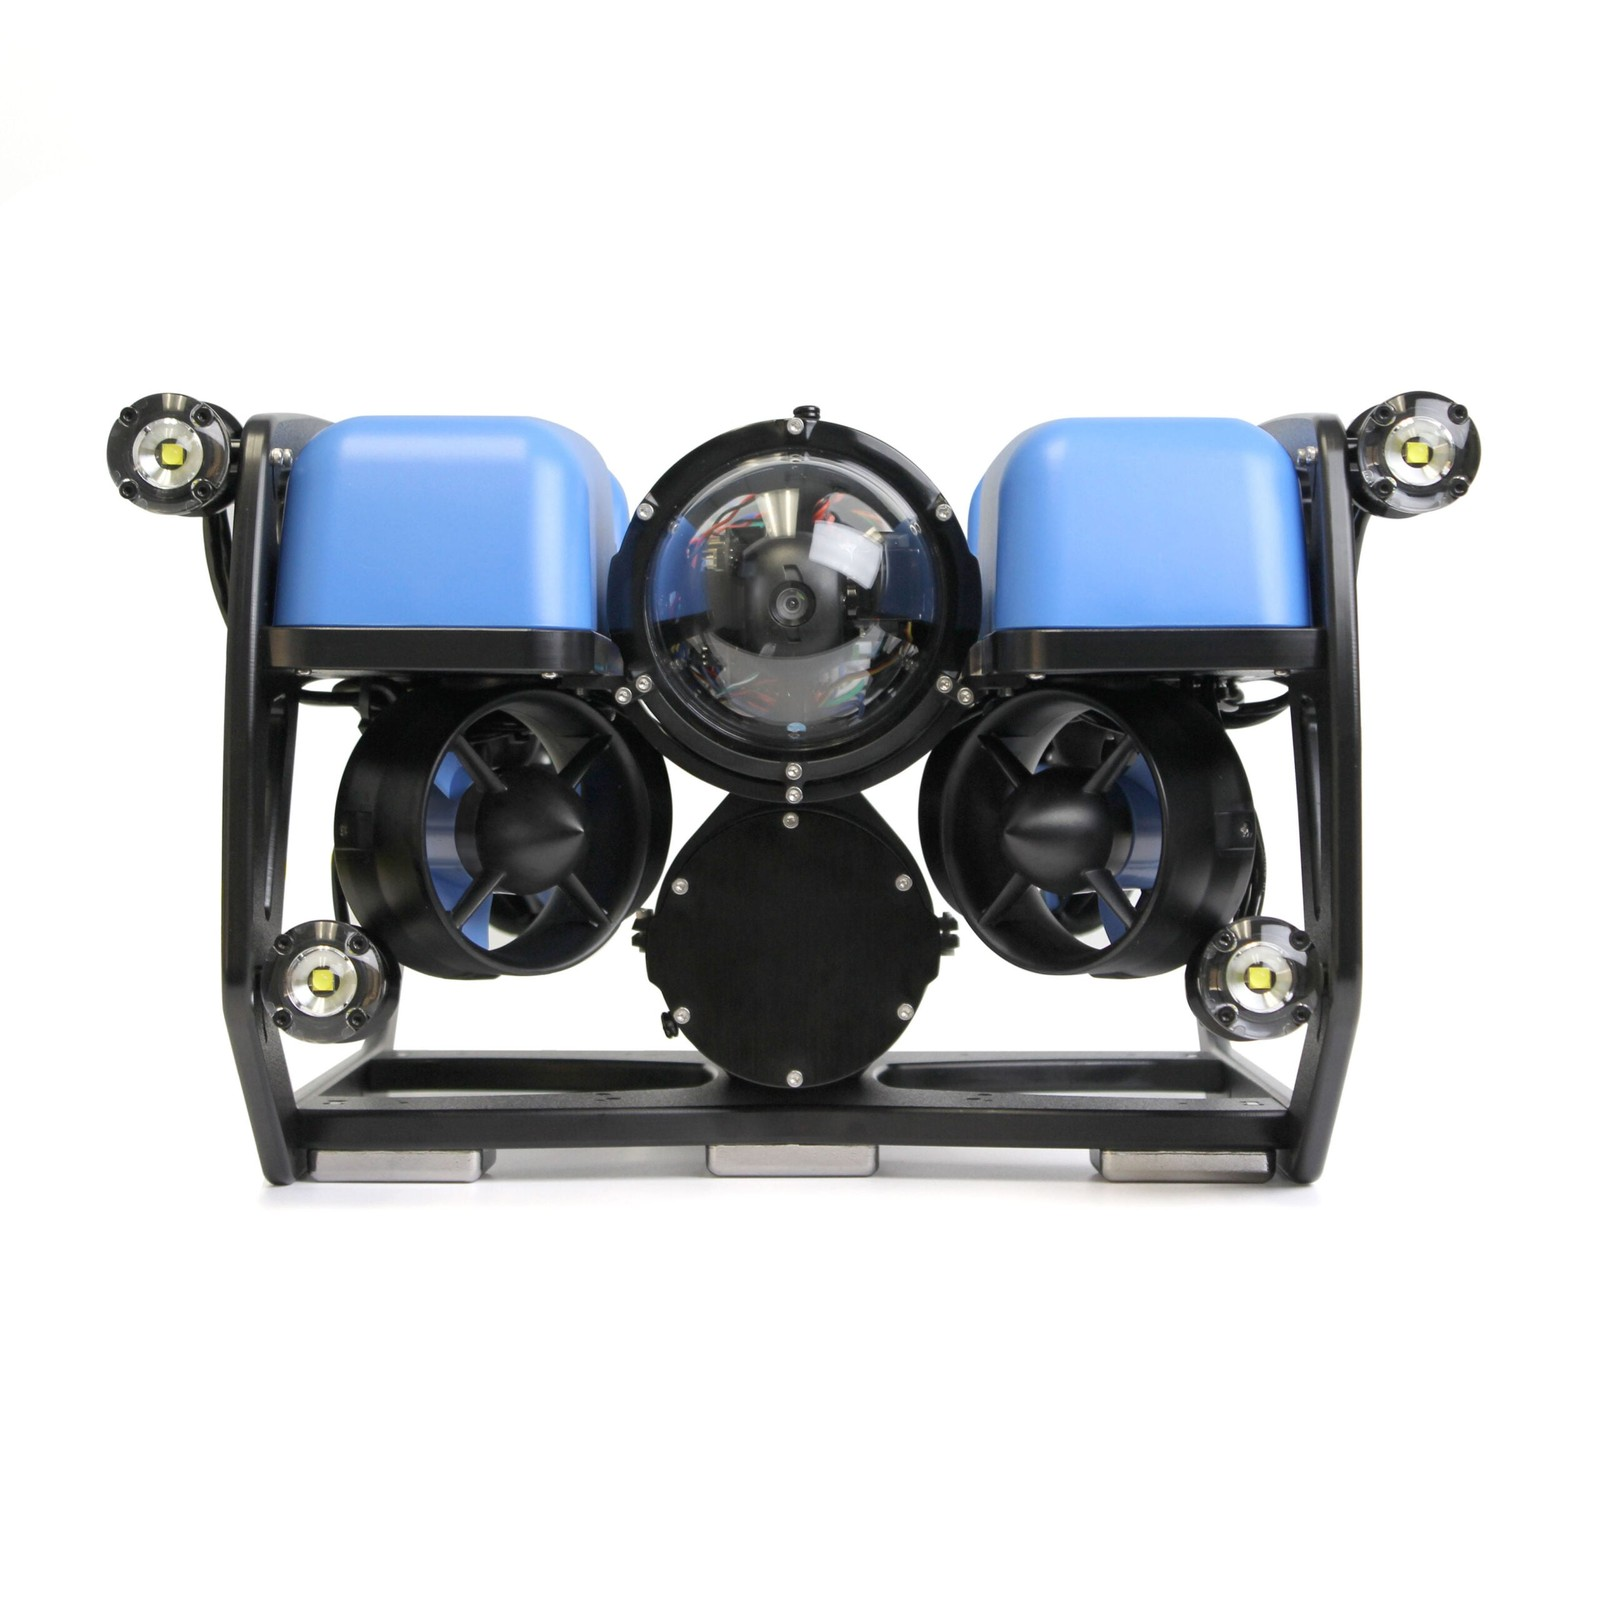
\includegraphics[height=2cm, keepaspectratio]{bluerov2.jpg}\\
        \vspace{0.2em}
        \tech{ROV}\\
        \tiny\textbf{BlueRobotics BlueROV2}\\
        \textit{Télé-opéré filaire}
      \end{center}
      \tiny
      6 DDL, stationnaire fin, inspection vidéo, prélèvements.
    \end{column}

    \begin{column}{0.19\textwidth}
      \begin{center}
        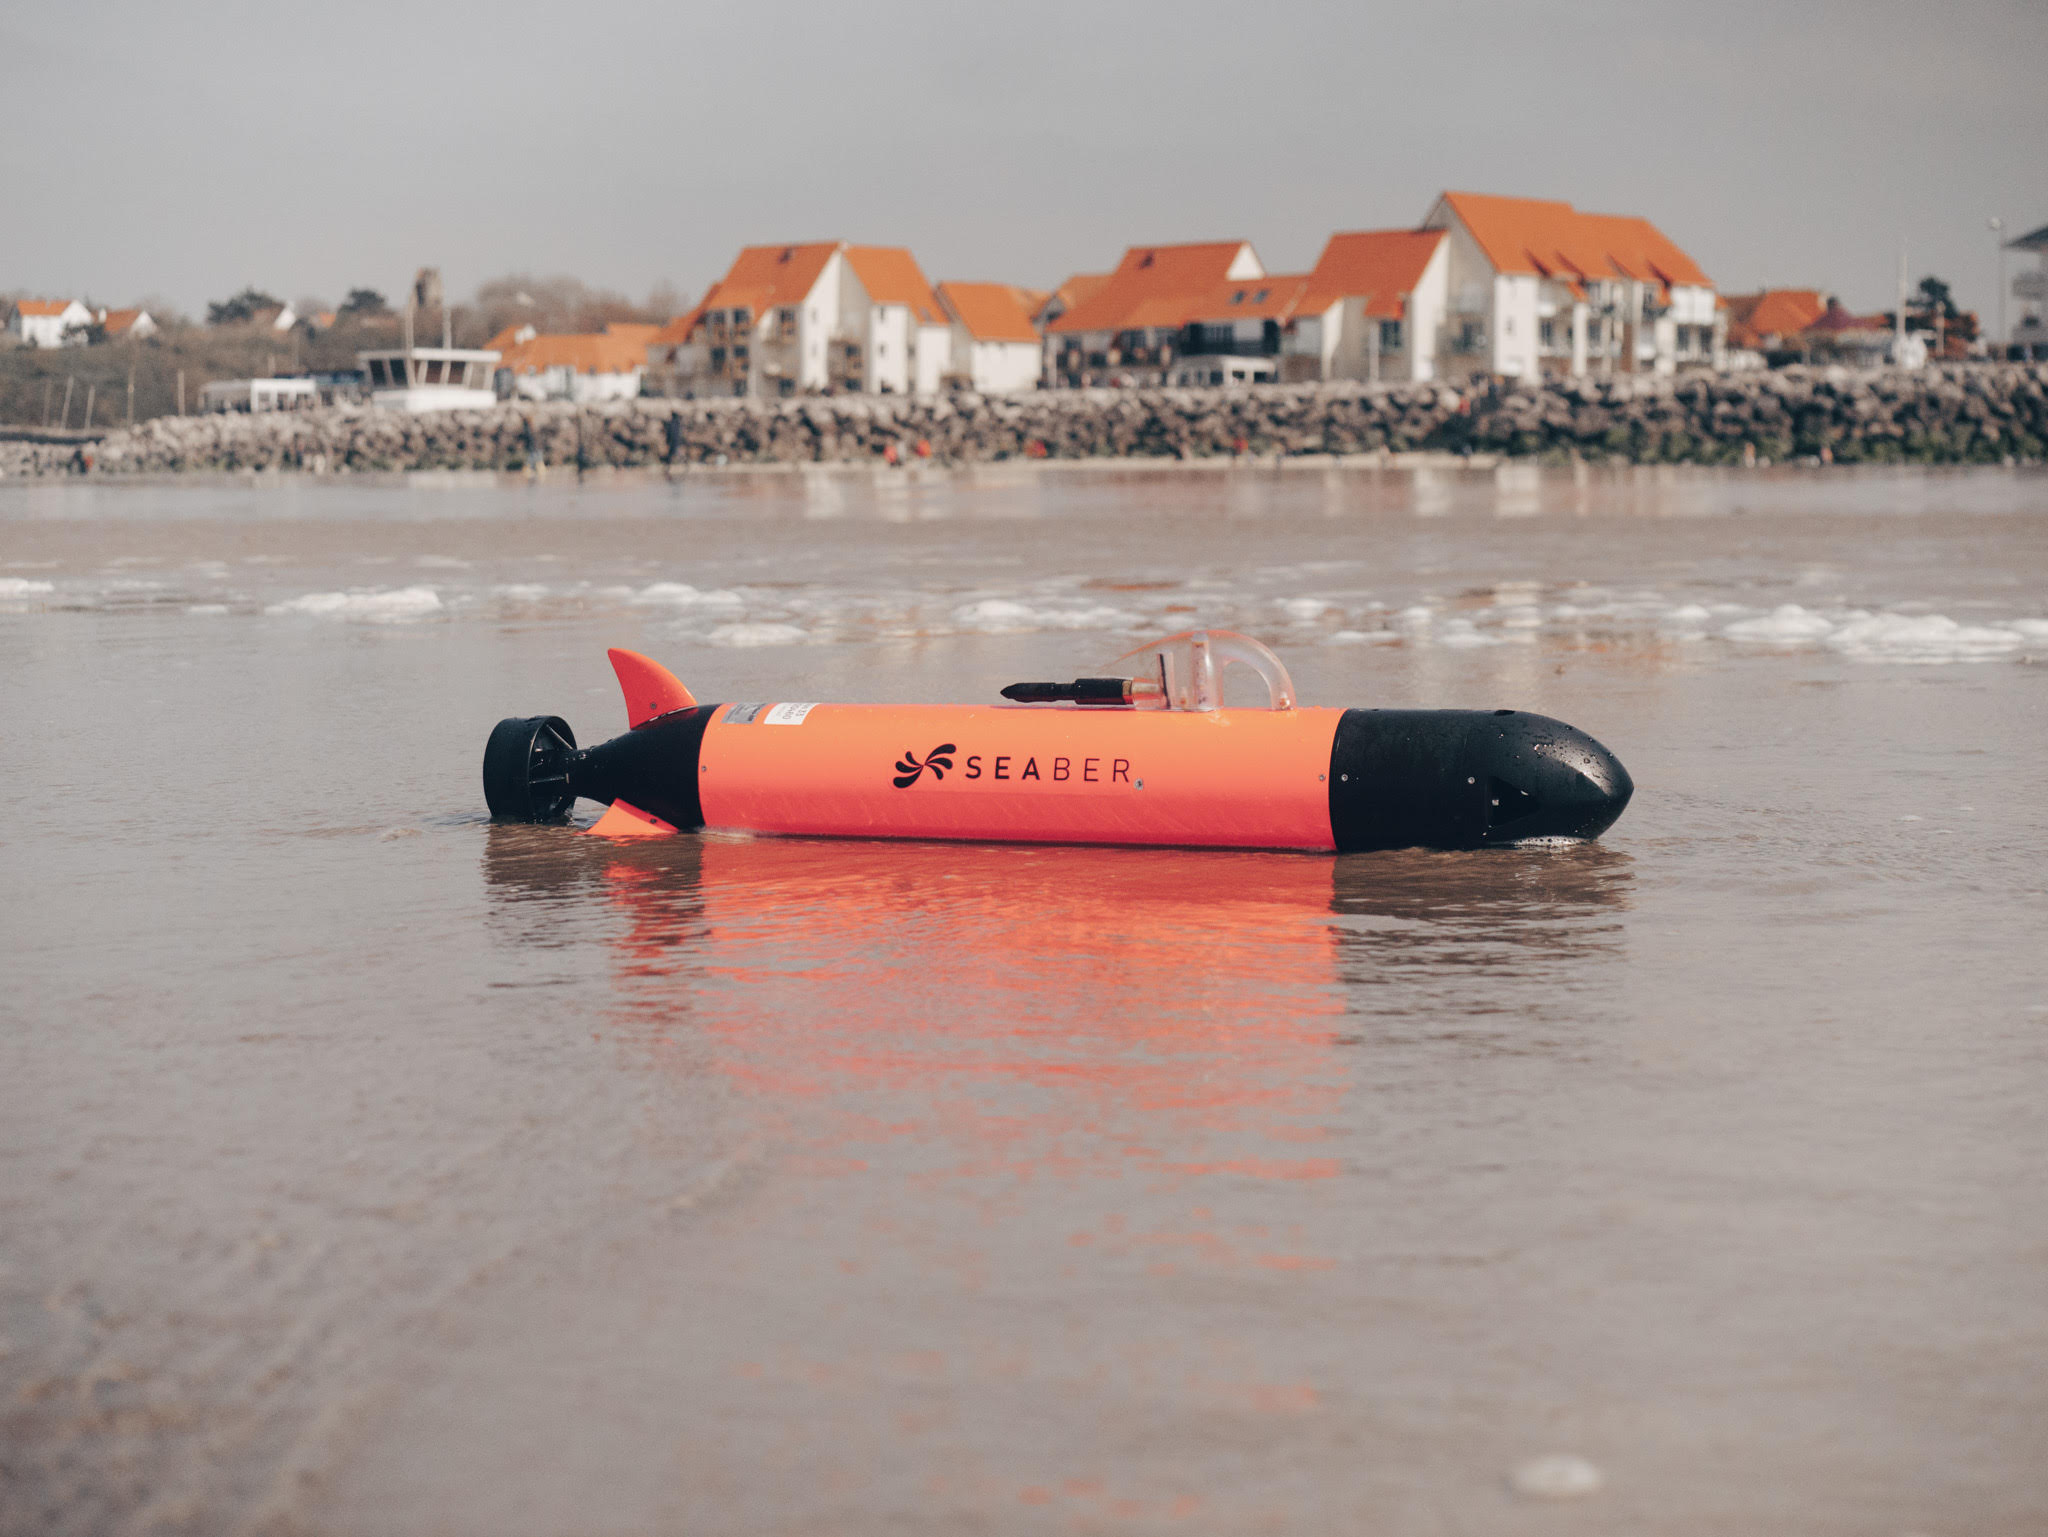
\includegraphics[height=2cm, keepaspectratio]{seaber_yuco.jpg}\\
        \vspace{0.2em}
        \tech{AUV}\\
        \tiny\textbf{Seaber YUCO}\\
        \textit{Autonome propulsé}
      \end{center}
      \tiny
      Transit $3\text{--}6\,\text{kts}$, profils yo-yo CTD, sonar latéral.
    \end{column}

    \begin{column}{0.19\textwidth}
      \begin{center}
        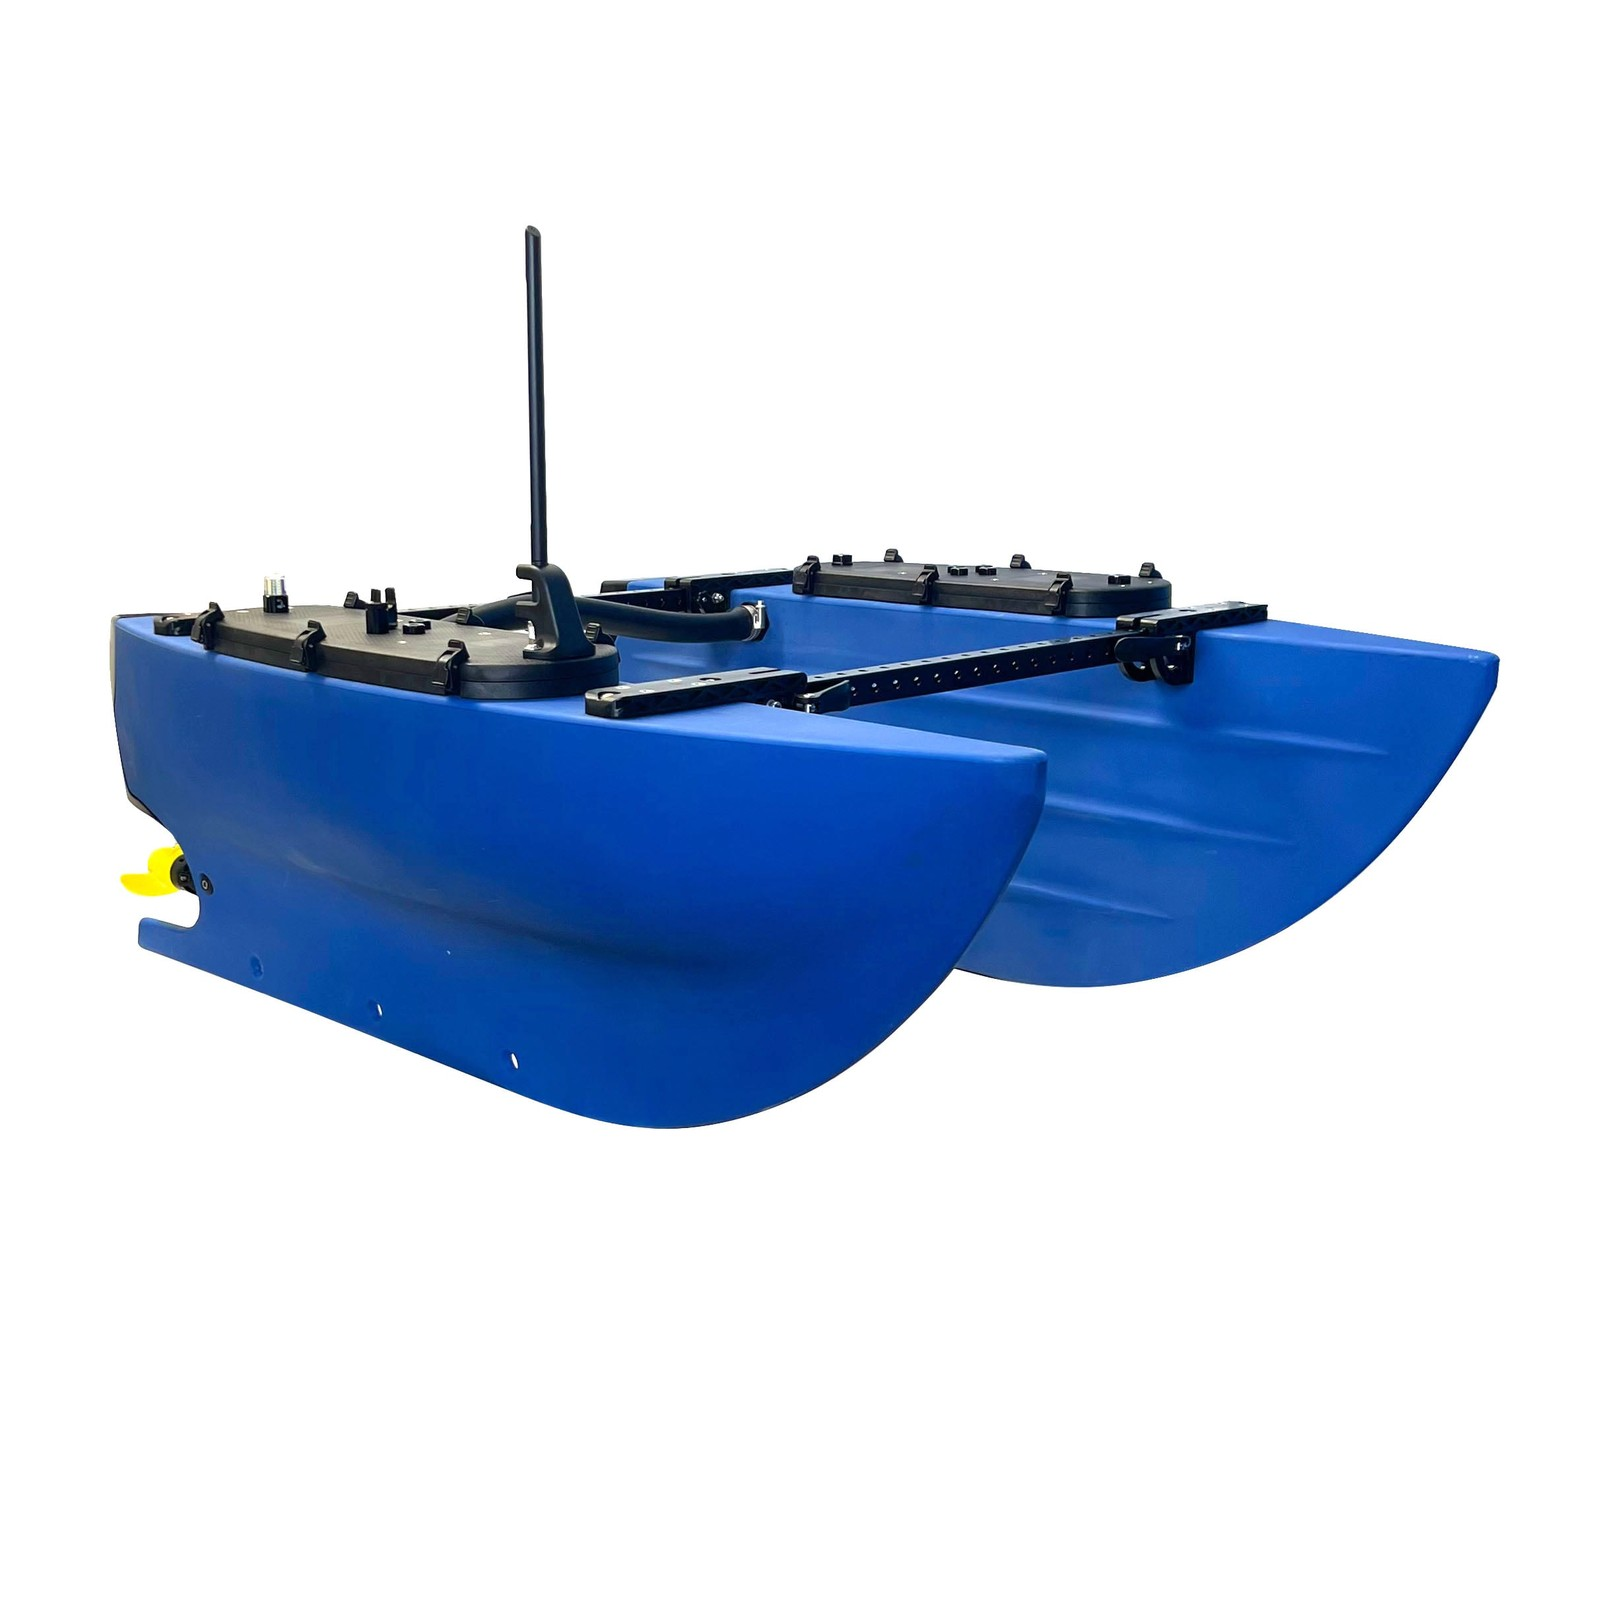
\includegraphics[height=2cm, keepaspectratio]{blueboat.jpg}\\
        \vspace{0.2em}
        \tech{ASV / USV}\\
        \tiny\textbf{BlueRobotics BlueBoat}\\
        \textit{Surface autonome}
      \end{center}
      \tiny
      GNSS, inspection de surface, bathymétrie fauchée mono/multi.
    \end{column}

    \begin{column}{0.21\textwidth}
      \begin{center}
        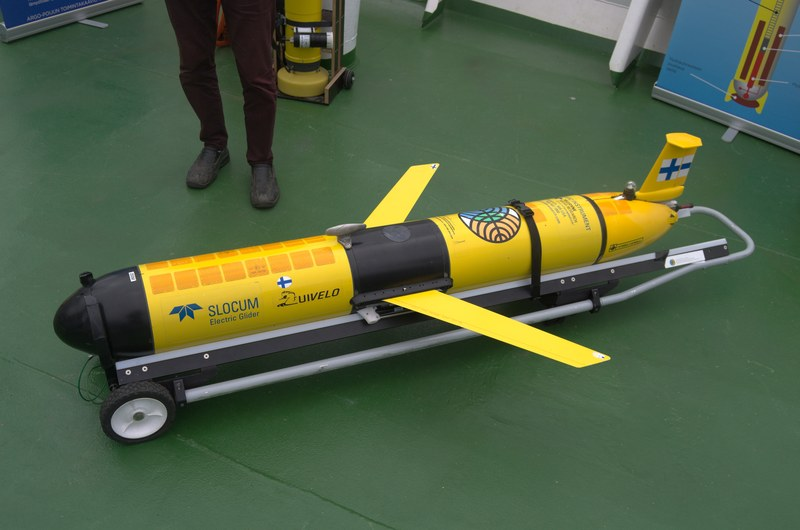
\includegraphics[height=2cm, keepaspectratio]{slocum_glider_clean.jpg}\\
        \vspace{0.2em}
        \succw{Glider}\\
        \tiny\textbf{Teledyne Slocum}\\
        \textit{Flottabilité variable}
      \end{center}
      \tiny
      Endurance plusieurs mois, sonde CTD, capteurs biochimiques, profils dents de scie transocéaniques.
    \end{column}

    \begin{column}{0.20\textwidth}
      \begin{center}
        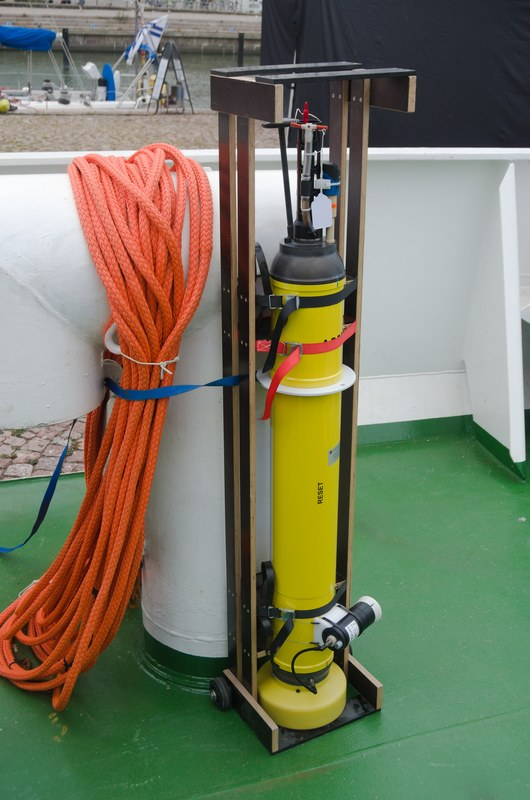
\includegraphics[height=2cm, keepaspectratio]{argo_float_clean.jpg}\\
        \vspace{0.2em}
        \alertw{Bouée Argo}\\
        \tiny\textbf{Teledyne Apex}\\
        \textit{Lagrangien profilant}
      \end{center}
      \tiny
      Cycles 10 jours, dérive $1000\,\text{m}$, 4 à 6 ans autonomie, sondes CTD, analyse des courants, capteurs biochimiques.
    \end{column}
  \end{columns}
\end{frame}

\begin{frame}{1.1b Zoom sur les Micro-AUVs : L'Exemple Seaber YUCO}
  \begin{columns}[c]
    \begin{column}{0.44\textwidth}
      \begin{center}
        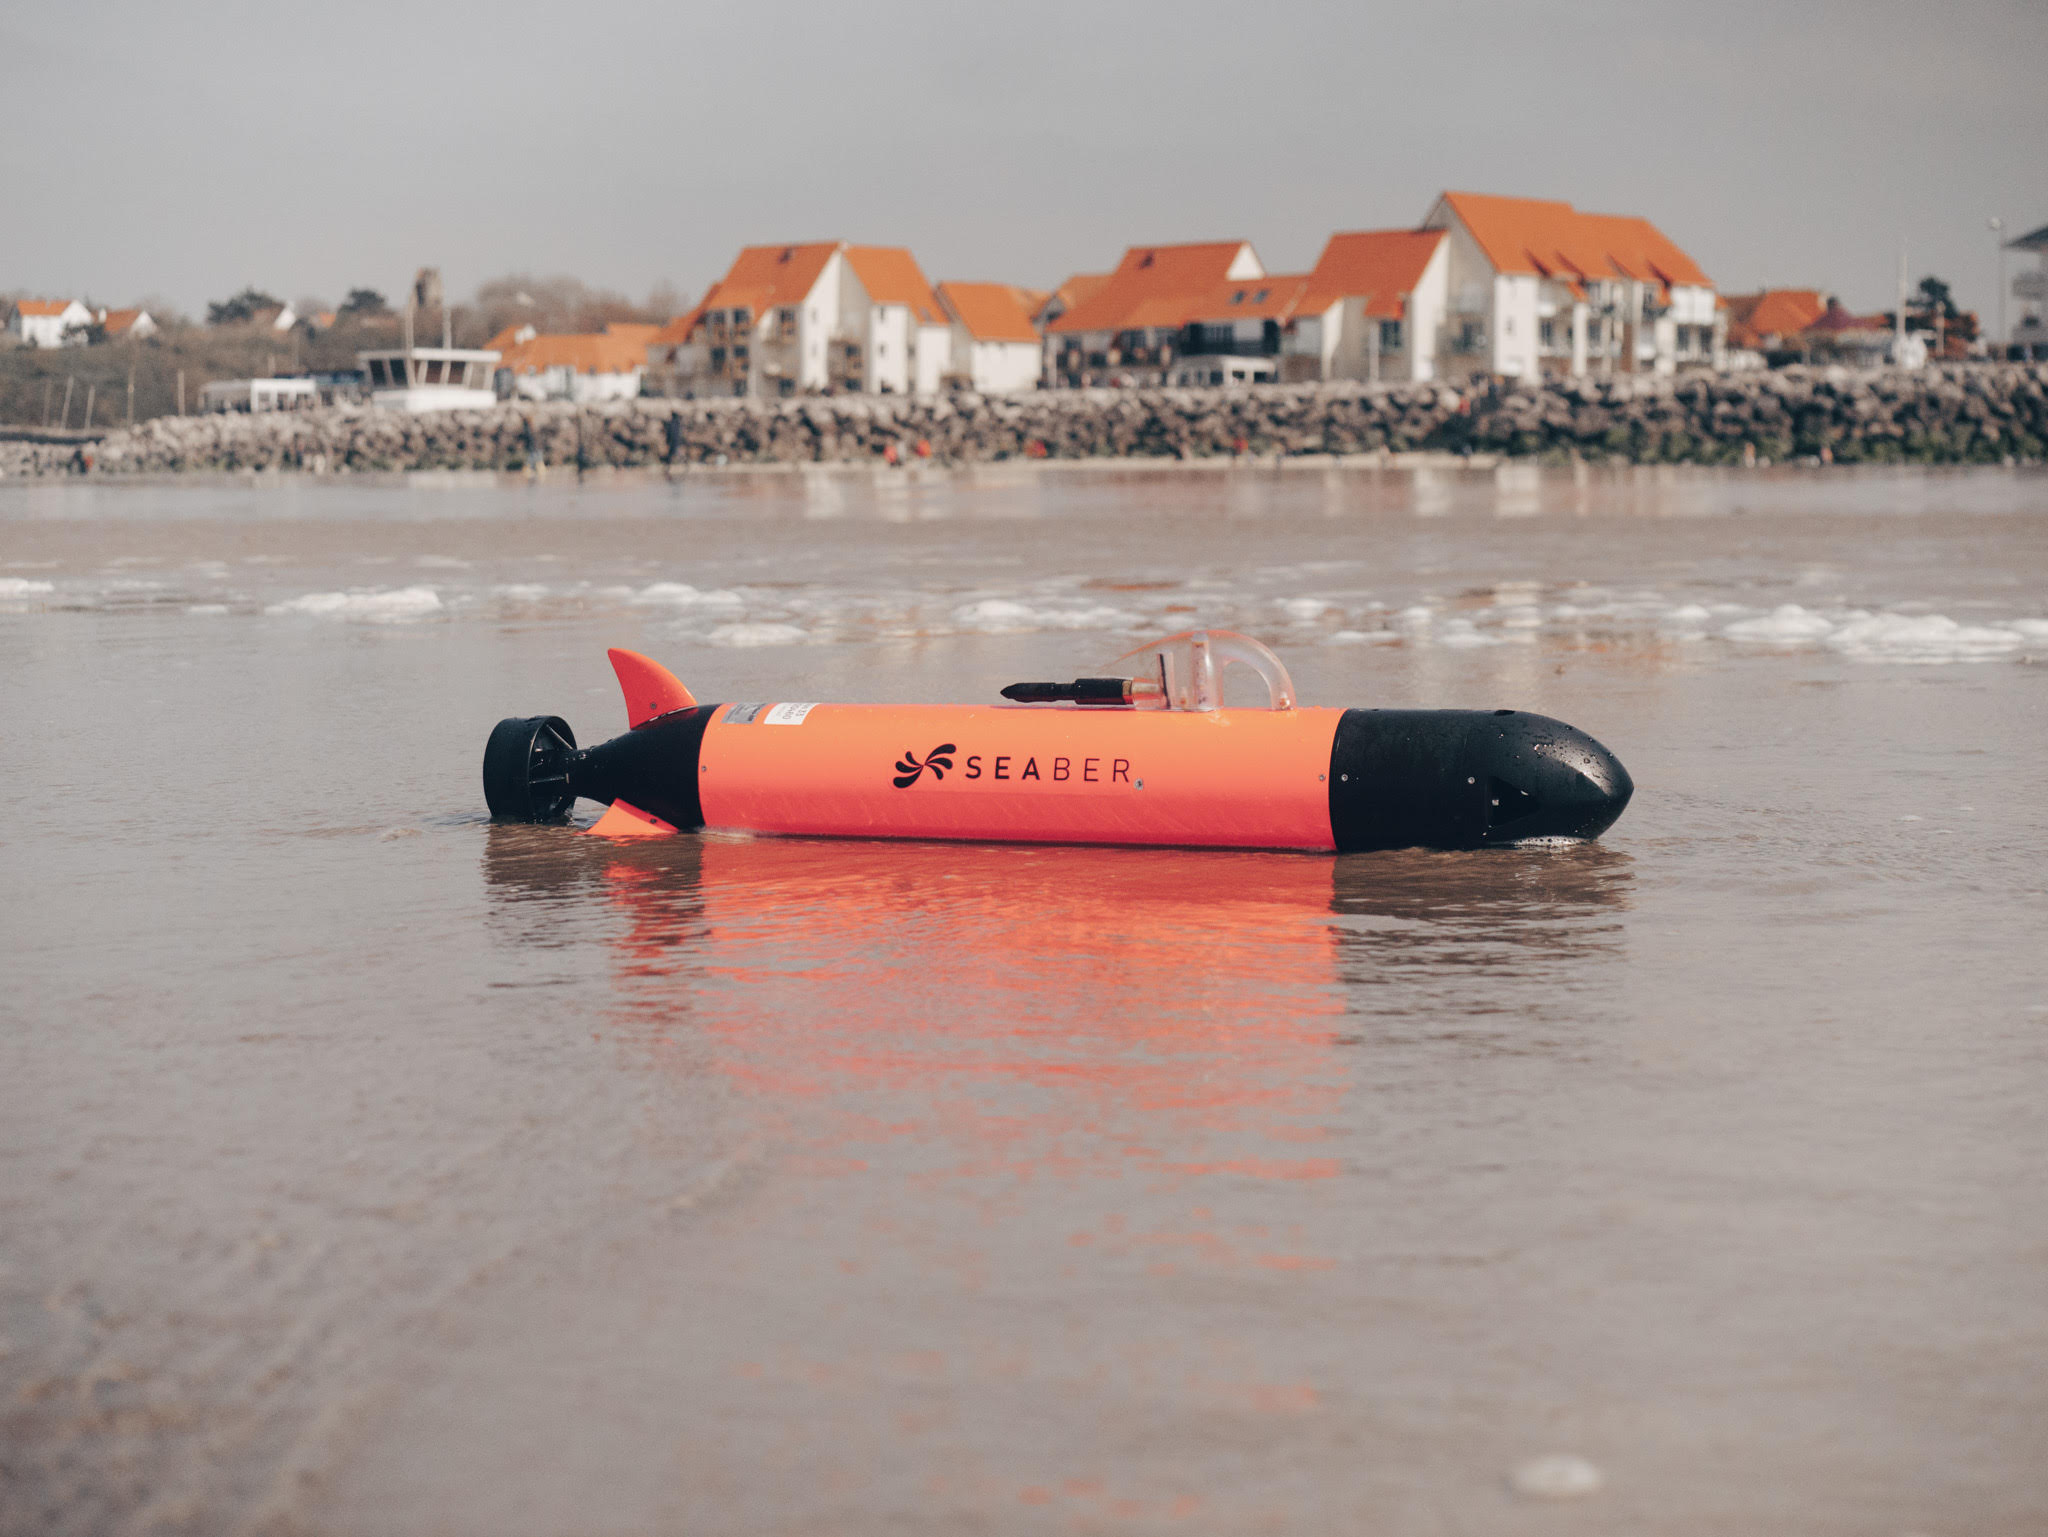
\includegraphics[width=\textwidth, height=3.0cm, keepaspectratio]{seaber_yuco.jpg}\\
        \vspace{0.2em}
        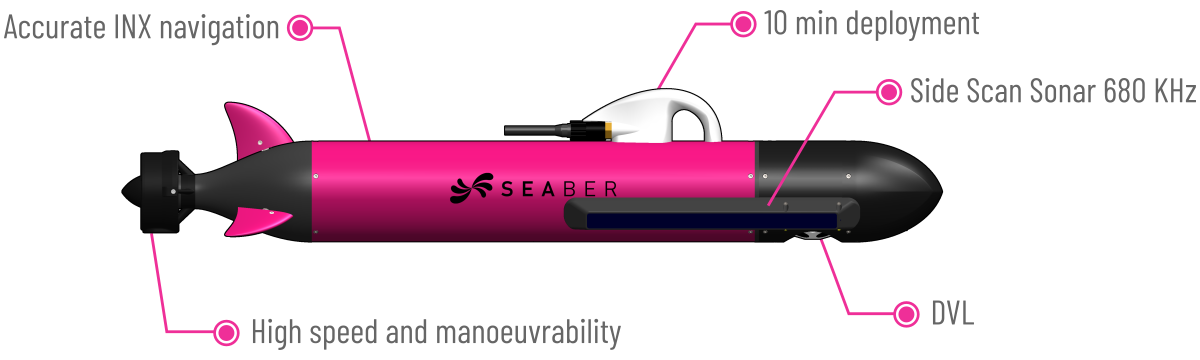
\includegraphics[width=\textwidth, height=1.45cm, keepaspectratio]{seaber_yuco_diagram.png}\\
        \vspace{0.1em}
        \scriptsize\textbf{Micro-AUV Seaber YUCO} (Lorient, France)\\
        \tiny\textit{Longueur $1\,\text{m}$ $\cdot$ Masse $10\,\text{kg}$ $\cdot$ Immersion $300\,\text{m}$ $\cdot$ Vitesse $3\text{--}6\,\text{kts}$}
      \end{center}
    \end{column}

    \begin{column}{0.54\textwidth}
      \begin{block}{\tech{La Révolution du Micro-AUV Côtier}}
        \scriptsize
        \begin{itemize}
          \item \textbf{Démocratisation} : déployable \succw{par 1 seul opérateur} (caisse de transport rigide compacte $<15\,\text{kg}$ tout compris).
          \item \textbf{Navigation inertielle INX©} : haute précision sans balisage acoustique lourd (LBL). Recalage fond par DVL-A50.
          \item \textbf{Autonomie \& Transit} : 8 à 10 h d'endurance, propulsion par hélice carénée et gouvernes arrière.
        \end{itemize}
      \end{block}

      \begin{exampleblock}{\tech{Déclinaisons Scientifiques \& Payloads}}
        \scriptsize
        \begin{itemize}
          \item \textbf{YUCO-CTD} : sonde Seabird/RBR en vol ondulant (\textit{yo-yo}).
          \item \textbf{YUCO-Scan} : sonar latéral ($680\,\text{kHz}$) pour cartographie benthique.
          \item \textbf{YUCO-Carrier / PAM} : capteurs sur mesure et écoute acoustique.
        \end{itemize}
      \end{exampleblock}
    \end{column}
  \end{columns}
\end{frame}

\begin{frame}{1.1b2 Zoom sur les Planeurs Sous-Marins : L'Exemple Slocum Glider}
  \begin{columns}[c]
    \begin{column}{0.42\textwidth}
      \begin{center}
        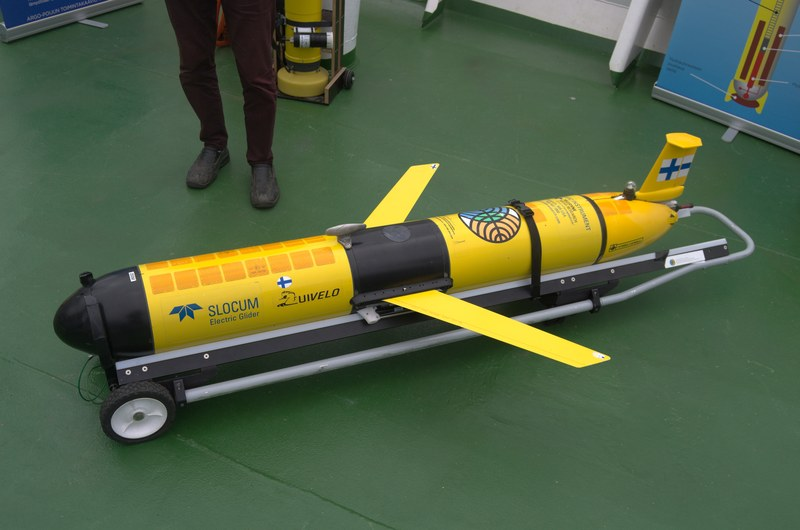
\includegraphics[width=\textwidth, height=3.6cm, keepaspectratio]{slocum_glider_clean.jpg}\\
        \vspace{0.2em}
        \small\textbf{Teledyne Webb Slocum G3 Glider}\\
        \scriptsize\textit{Planeur sous-marin océanographique autonome}
      \end{center}
    \end{column}

    \begin{column}{0.56\textwidth}
      \begin{block}{\succw{Principe de Propulsion par Flottabilité Variable}}
        \scriptsize
        \begin{itemize}
          \item \textbf{Moteur de flottabilité} : une pompe hydraulique transfère de l'huile entre un réservoir interne et une vessie externe.
          \item \textbf{Conversion d'Archimède en poussée} : la variation de volume fait couler ou flotter l'engin ; les ailes fixes transforment ce mouvement vertical en vitesse horizontale (trajectoire en dents de scie).
          \item \textbf{Pas d'actionneurs en continu} : très faible consommation électrique ($\approx 1\text{--}2\,\text{W}$ moyen), quasi-silencieux (idéal acoustique passive).
        \end{itemize}
      \end{block}

      \begin{exampleblock}{\tech{Caractéristiques Techniques \& Missions}}
        \scriptsize
        \begin{itemize}
          \item \textbf{Vitesse} : $0.5\text{--}1\,\text{n\oe ud}$ ($0.25\text{--}0.5\,\text{m/s}$) $\cdot$ \textbf{Immersion} : $200\,\text{m}$ à $1000\,\text{m}$ ($6000\,\text{m}$ Deep).
          \item \textbf{Autonomie} : \succw{Plusieurs semaines à 1 an} ($>4\,000\text{--}10\,000\,\text{km}$).
          \item \textbf{Surfaçage \& Comms} : antenne dans l'empennage relevé en surface pour recalage GNSS et transmission satellite Iridium bidirectionnelle.
          \item \textbf{Capteurs} : CTD, oxygène dissous ($O_2$), chlorophylle, turbidité, écoute acoustique passive pour cétacés.
        \end{itemize}
      \end{exampleblock}
    \end{column}
  \end{columns}
\end{frame}

\begin{frame}{1.1b3 Zoom sur les Flotteurs Profilants Dérivants : Le Réseau Argo}
  \begin{columns}[c]
    \begin{column}{0.40\textwidth}
      \begin{center}
        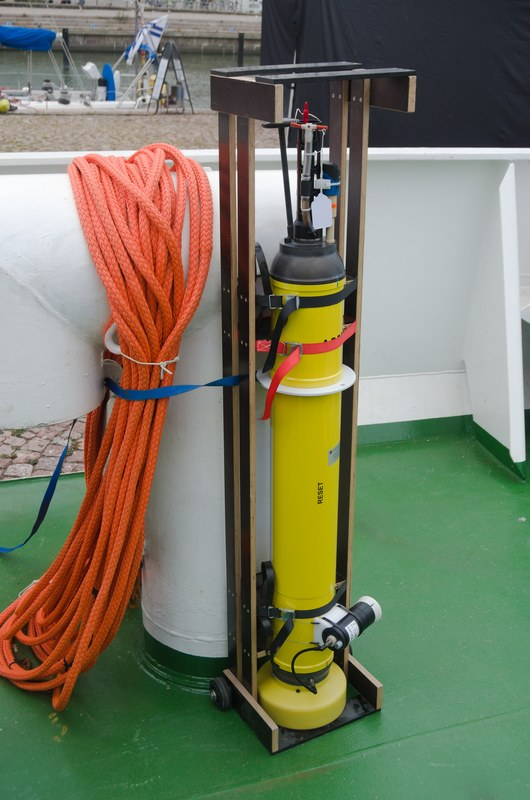
\includegraphics[width=\textwidth, height=4.5cm, keepaspectratio]{argo_float_clean.jpg}\\
        \vspace{0.2em}
        \small\textbf{Flotteur Profilant Dérivant (Argo)}\\
        \scriptsize\textit{Modèles Provor / Arvor (NKE/Ifremer) ou Apex / Navis}
      \end{center}
    \end{column}

    \begin{column}{0.58\textwidth}
      \begin{block}{\alertw{Principe de Fonctionnement}}
        \scriptsize
        \begin{enumerate}
          \item \textbf{Plongée profonde} : descente jusqu'à $2000\,\text{m}$ (ou $4000\text{--}6000\,\text{m}$ pour Deep Argo).
          \item \textbf{Remontée profilante} : ascension continue vers la surface en enregistrant la colonne d'eau (température, salinité, pression).
          \item \textbf{Surfaçage \& Télétransmission} : transmission des profils par satellite (Iridium), positionnement GPS, puis purge et nouvelle plongée.
        \end{enumerate}
      \end{block}

      \begin{exampleblock}{\tech{Caractéristiques Clés \& Impact Scientifique}}
        \scriptsize
        \begin{itemize}
          \item \textbf{Autonomie} : \succw{4 à 6 ans en mer} ($\approx 150\text{--}250$ cycles complets) sur piles Lithium.
          \item \textbf{Réseau mondial} : \textbf{$\approx 4\,000$ flotteurs actifs} en permanence dans tous les océans (données ouvertes en temps réel).
          \item \textbf{Payload métrologique} : sonde CTD haute précision (Seabird SBE41CP), capteurs BGC-Argo ($O_2$, pH, nitrates, Chl-a).
          \item \textbf{Applications} : climatologie globale, bilan thermique océanique, calibration altimétrie spatiale (Copernicus, SWOT).
        \end{itemize}
      \end{exampleblock}
    \end{column}
  \end{columns}
\end{frame}

\begin{frame}{1.1c Ordres de Grandeur des Coûts d'Acquisition (Porteurs $\approx 1\,\text{m}$)}
  \scriptsize
  \begin{table}[h]
    \centering
    \begin{tabularx}{\textwidth}{l p{2.6cm} p{2.2cm} p{2.8cm} X}
      \toprule
      \textbf{Famille} & \textbf{Modèle Réf.} & \textbf{Porteur Nu / Base} & \textbf{Équipé Recherche} & \textbf{Alternative Ind. / Défense} \\
      \midrule
      \rowcolor{OceanGray}
      \tech{ROV} \tiny(Filaire) & BlueROV2 Heavy \tiny(BlueRobotics, US) & $\approx \mathbf{4{,}5\text{--}6\,\text{k€}}$ & $\approx \mathbf{8\text{--}15\,\text{k€}}$ \tiny(Fathom $150\,\text{m}$, console, pince, DVL opt.) & $>40\text{--}120\,\text{k€}$ \tiny(VideoRay Defender, Deep Trekker Pivot) \\
      \tech{ASV / USV} \tiny(Surface) & BlueBoat \tiny(BlueRobotics, US) & $\approx \mathbf{3{,}5\text{--}5\,\text{k€}}$ & $\approx \mathbf{7\text{--}18\,\text{k€}}$ \tiny(GNSS, sondeur Ping ou MBES Cerulean) & $>50\text{--}250\,\text{k€}$ \tiny(OceanAlpha SL40, Exail DriX, Maritime Robotics Otter) \\
      \rowcolor{OceanGray}
      \tech{Micro-AUV} & Seaber YUCO \tiny(Seaber, FR) & $\approx \mathbf{25\text{--}35\,\text{k€}}$ \tiny(Carrier intégration) & $\approx \mathbf{35\text{--}75\,\text{k€}}$ \tiny(YUCO-CTD / Scan avec DVL et acoustique) & $>150\text{--}500\,\text{k€}$ \tiny(Gavia, REMUS 100, Exail A18) \\
      \bottomrule
    \end{tabularx}
  \end{table}

  \vspace{0.2em}
  \begin{columns}[T]
    \begin{column}{0.48\textwidth}
      \begin{block}{\tech{Pourquoi de Tels Écarts de Prix ?}}
        \begin{itemize}
          \item Les briques open-source (ArduSub/ArduRover) et composants modulaires divisent le coût d'accès par un facteur $3$ à $10\times$.
          \item Les systèmes industriels/défense intègrent une certification militaire, redondance totale et SAV sur site à coût élevé.
        \end{itemize}
      \end{block}
    \end{column}

    \begin{column}{0.50\textwidth}
      \begin{block}{\succw{Impact Budgétaire de la Charge Utile}}
        \begin{itemize}
          \item Les capteurs scientifiques (DVL-A50 : $\approx 7\,\text{k€}$, sondeur MBES Cerulean : $\approx 8\,\text{k€}$, sonde CTD calibrée : $\approx 8\text{--}15\,\text{k€}$) représentent souvent \succw{$50\%$ à $70\%$ du coût global} du vecteur !
          \item Penser aux accessoires : ombilicaux, valises étanches, batteries de rechange, consoles terrain durcies.
        \end{itemize}
      \end{block}
    \end{column}
  \end{columns}
\end{frame}

\begin{frame}{1.1d Écosystème Industriel : Constructeurs Clés \& Revendeurs Français}
  \begin{columns}[T]
    \begin{column}{0.50\textwidth}
      \begin{block}{\tech{Constructeurs Mondiaux ($\approx 1\,\text{m}$ / Portables)}}
        \scriptsize
        \begin{itemize}
          \item \textbf{BlueRobotics} \textit{(USA)} : leader matériel modulaire open-source (BlueROV2, BlueBoat, T200, WetLink, BlueOS).
          \item \textbf{Seaber} \textit{(France - Lorient)} : pionnier des micro-AUVs côtiers légers (gamme YUCO $<10\,\text{kg}$, navigation INX©).
          \item \textbf{RTSYS} \textit{(France - Lorient)} : micro-AUVs acoustiques (NemoSens), modems et balises sous-marines.
          \item \textbf{Deep Trekker} \textit{(Canada)} : ROVs d'inspection robustes (DTG3, Pivot, Revolution).
          \item \textbf{Chasing / QYSEA} \textit{(Chine)} : ROVs d'inspection compacts légers (Chasing M2 Pro, Fifish V6).
          \item \textbf{Water Linked} \textit{(Norvège)} : capteurs acoustiques miniaturisés (DVL-A50, Underwater GPS USBL).
        \end{itemize}
      \end{block}
    \end{column}

    \begin{column}{0.48\textwidth}
      \begin{block}{\succw{Revendeurs \& Intégrateurs en France}}
        \scriptsize
        \textit{Canaux marchés publics CNRS/Univ (Chorus Pro, support \& SAV) :}
        \begin{itemize}
          \item \textbf{SyERA} \textit{(Belgentier / Toulon)} : distributeur officiel BlueRobotics, support, durcissement et personnalisations R\&D/défense.
          \item \textbf{ROV Expert} \textit{(Béziers)} : distributeur majeur BlueRobotics (Top 5 mondial), kits montés, pièces, intégration capteurs \& SAV.
          \item \textbf{Subsea Tech} \textit{(Marseille)} : distributeur BlueRobotics, intégrateur sonars/caméras et fabricant USV (SeaCat).
          \item \textbf{MacArtney France} \textit{(Aix-en-Provence)} : connectique SubConn, sonars et instrumentation océanographique.
          \item \textbf{Seaber} \textit{(Lorient)} : constructeur français, vente directe, support recherche et essais en mer.
        \end{itemize}
      \end{block}
    \end{column}
  \end{columns}
\end{frame}

\begin{frame}{1.2 Anatomie d'une Plateforme de Recherche : Le BlueROV2}
  \begin{columns}[c]
    \begin{column}{0.45\textwidth}
      \begin{center}
        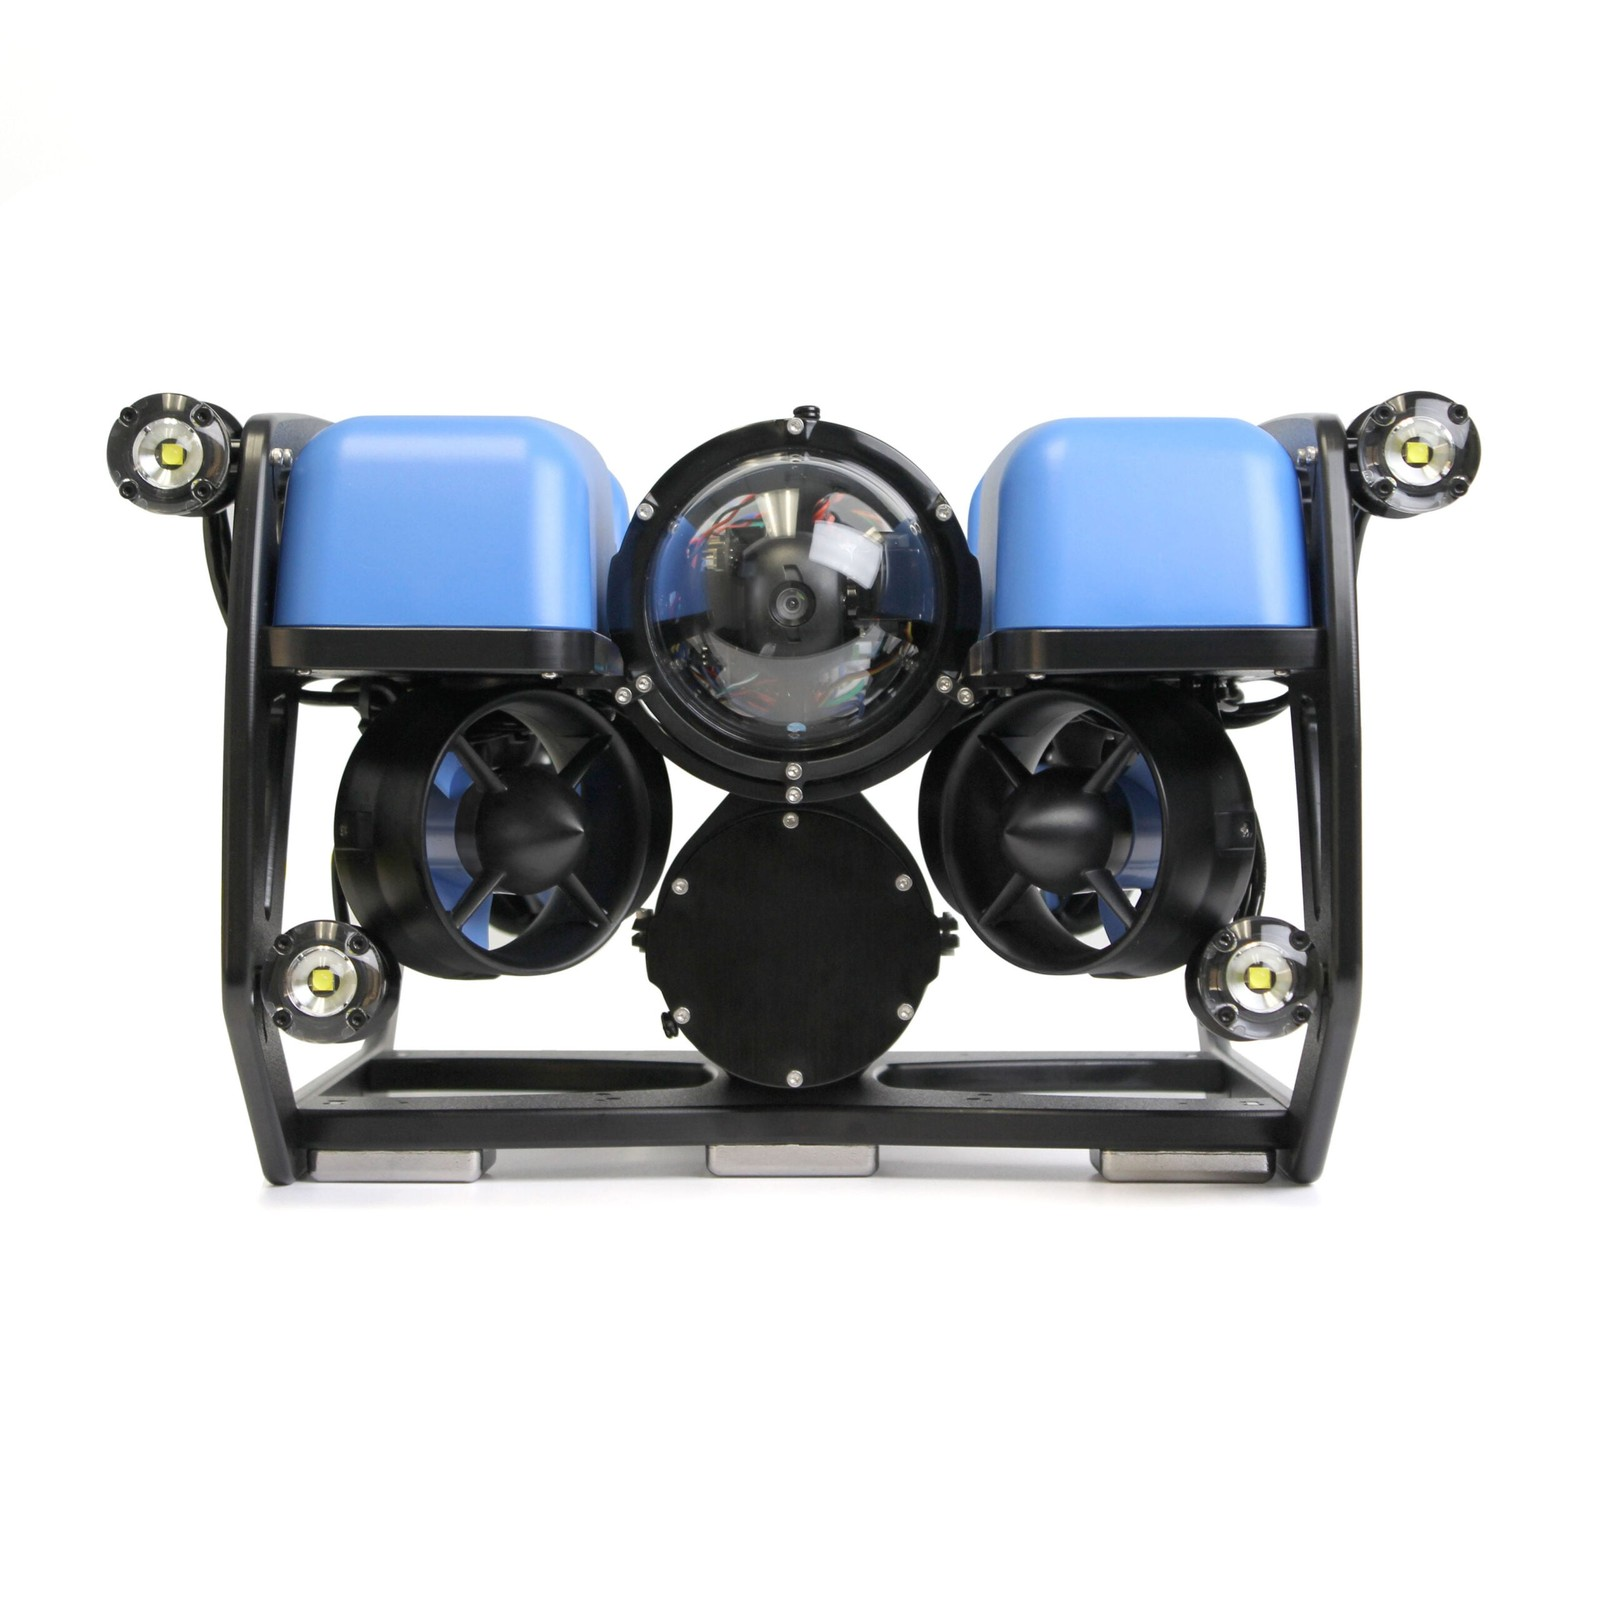
\includegraphics[width=\textwidth, height=4.2cm, keepaspectratio]{bluerov2.jpg}\\
        \vspace{0.2em}
        \small\textbf{BlueROV2} (BlueRobotics)\\
        \scriptsize\textit{Châssis modulaire PEHD, 8 propulseurs vectorisés, double caisson étanche}
      \end{center}
    \end{column}

    \begin{column}{0.53\textwidth}
      \begin{block}{\tech{Architecture Matérielle Découplée}}
        \scriptsize
        \begin{itemize}
          \item \textbf{Caisson Électronique (Tube 4")} : RPi 4/5, carte Navigator, modem Fathom-X, \succw{caméra Low-Light HD sur nacelle tilt}.
          \item \textbf{Caisson Batterie (Tube 3")} : Li-ion 4S $14.8\,\text{V}$ $18\text{Ah}$, interrupteur étanche \& fusible.
          \item \textbf{Capteurs de Sûreté Véhicule} : \alertw{SOS Leak Sensors} (détection fuite fond de tubes) \& capteur de dépression interne.
          \item \textbf{Capteurs \& Indicateurs de Mission} : Pression/profondeur \textbf{Bar30}, \succw{projecteurs étanches Lumen ($2\times 1500\,\text{lm}$)}.
          \item \textbf{Actionnement \& Traversées} : 6 à 8 moteurs \textbf{T200}, pénétrateurs \textbf{WetLink} ou connecteurs \textbf{Cobalt/SubConn}.
          \item \textbf{Ombilical} pour téléopération et transfert de données.
        \end{itemize}
      \end{block}
    \end{column}
  \end{columns}
\end{frame}

\begin{frame}{1.2b L'Énergie Embarquée : Pourquoi Enfermer la Batterie ?}
  \begin{columns}[c]
    \begin{column}{0.42\textwidth}
      \begin{center}
        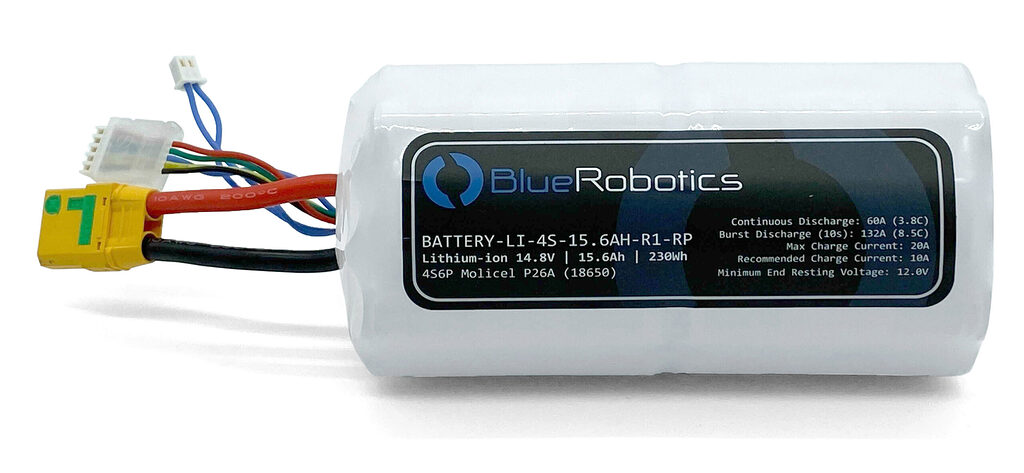
\includegraphics[width=\textwidth, height=2.4cm, keepaspectratio]{battery_pack.jpg}\\
        \vspace{0.2em}
        \tech{Batterie Li-ion 4S ($14.8\,\text{V}$, $15.6\,\text{Ah}$ / $230\,\text{Wh}$)}\\
        \scriptsize\textit{Logée dans un caisson 3" dédié sous le robot}
      \end{center}
      \scriptsize
      \begin{block}{\succw{Avantages de l'Énergie Embarquée}}
        \begin{itemize}
          \item \textbf{Stabilité} : masse lourde ($1.2\,\text{kg}$) au point le plus bas $\rightarrow$ abaisse $G$ et maximise $\overline{BG}$.
          \item \textbf{Courant crête instantané} : jusqu'à \alertw{$132\,\text{A}$} disponibles sans chute de tension.
        \end{itemize}
      \end{block}
    \end{column}

    \begin{column}{0.56\textwidth}
      \textbf{Pourquoi ne pas alimenter en 14.8V depuis la surface ?}
      \scriptsize
      \begin{itemize}
        \item Consommation de 6 à 8 thrusters T200 : $I = \mathbf{30\text{ à }60\,\text{A}}$.
        \item Ombilical fin neutre ($100\text{ à }300\,\text{m}$) : résistance $R \approx 1.5\text{ à }4\,\Omega$.
      \end{itemize}

      \vspace{0.2em}
      \begin{alertblock}{La Chute de Tension Ohmique ($\Delta V = R \cdot I$)}
        \scriptsize
        \[
          \Delta V = 2\,\Omega \times 30\,\text{A} = \mathbf{60\,\text{V}} \quad (\gg 14.8\,\text{V} !)
        \]
        La tension arrivant au robot serait \alertw{négative ou quasi-nulle} ! Les moteurs caleraient instantanément.
      \end{alertblock}

      \begin{alertblock}{Les Pertes Joule Destructrices ($P = R \cdot I^2$)}
        \scriptsize
        \[
          P_{\text{perte}} = 2\,\Omega \times (30\,\text{A})^2 = \mathbf{1800\,\text{W}}
        \]
        L'énergie serait dissipée en pure chaleur dans le câble $\rightarrow$ \alertw{fusion de l'ombilical} !
      \end{alertblock}
    \end{column}
  \end{columns}
\end{frame}

\begin{frame}{1.3 L'Actionnement Réel : Le Propulseur Brushless T200}
  \begin{columns}[c]
    \begin{column}{0.62\textwidth}
      \textbf{Pourquoi le T200 est-il unique ?}
      \scriptsize
      \begin{itemize}
        \item \textbf{Moteur noyé (Flooded)} : l'eau de mer circule librement à l'intérieur $\rightarrow$ \succw{refroidissement direct des bobinages}.
        \item \textbf{Encapsulation résine époxy} : stator surmoulé sous vide.
        \item \textbf{Paliers autolubrifiants PEEK} : zéro roulement métallique.
        \item \textbf{Aimants néodyme scellés} : revêtement époxy anticorrosion.
      \end{itemize}

      \vspace{0.2em}
      \begin{block}{Performances \& Contrôleurs ESC}
        \scriptsize
        \begin{itemize}
          \item Poussée T200 : jusqu'à \textbf{$5.25\,\text{kgf}$} ($14.8\,\text{V}$ / Li-ion 4S).
          \item \tech{Basic ESC (30A)} : $7\text{--}26\,\text{V}$, $50\,\text{A}$ continu, dissipation accrue pour caisson fermé.
          \item \succw{Commande réversible} : PWM bidirectionnel ($1100\,\mu\text{s}$ AR -- $1500\,\mu\text{s}$ Stop -- $1900\,\mu\text{s}$ AV).
        \end{itemize}
      \end{block}
    \end{column}

    \begin{column}{0.35\textwidth}
      \begin{center}
        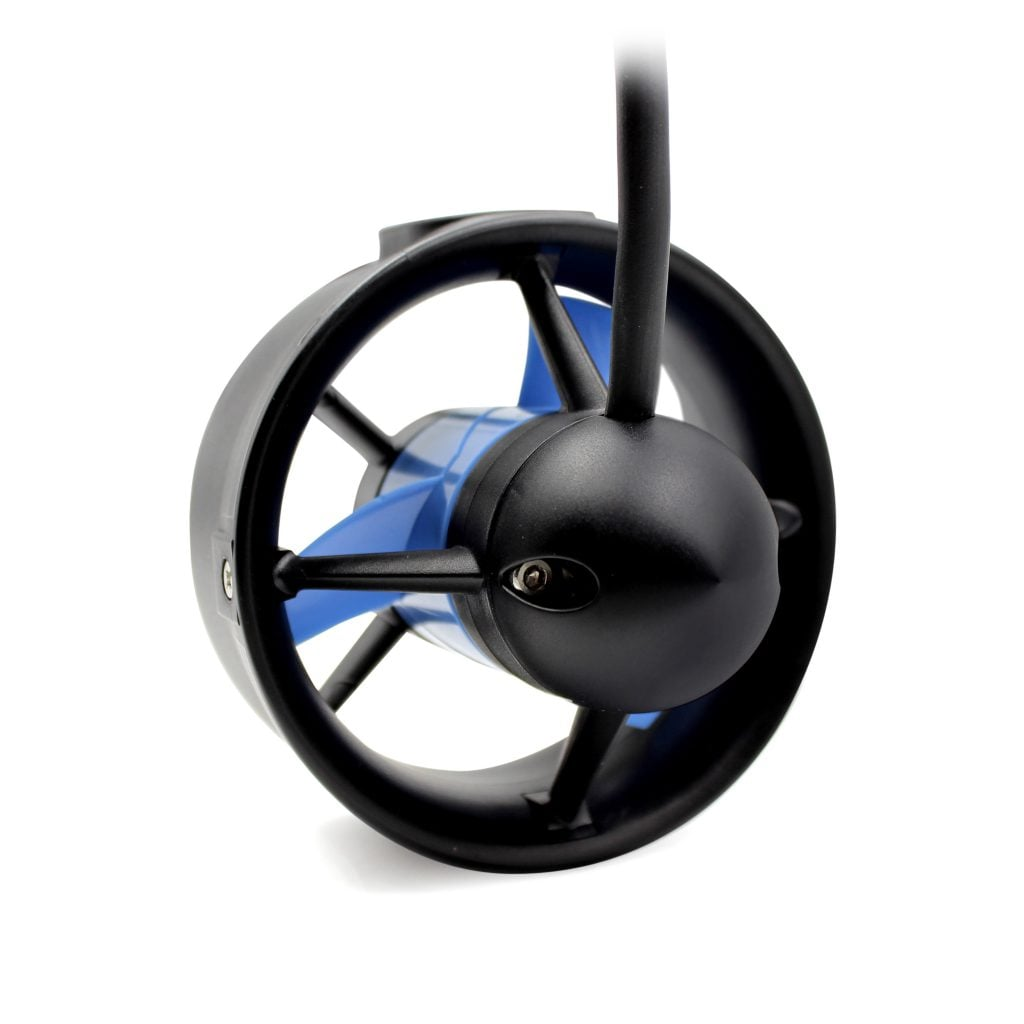
\includegraphics[height=3.2cm, keepaspectratio]{t200_thruster.png}\\
        \vspace{0.2em}
        \footnotesize\textbf{Propulseur T200}\\
        \scriptsize\textit{Stator noyé \& hélice polycarbonate}
      \end{center}
    \end{column}
  \end{columns}
\end{frame}

\begin{frame}{1.3b Panorama des Actionneurs Marins : T200, T500 \& Servos}
  \begin{columns}[T]
    \begin{column}{0.32\textwidth}
      \begin{center}
        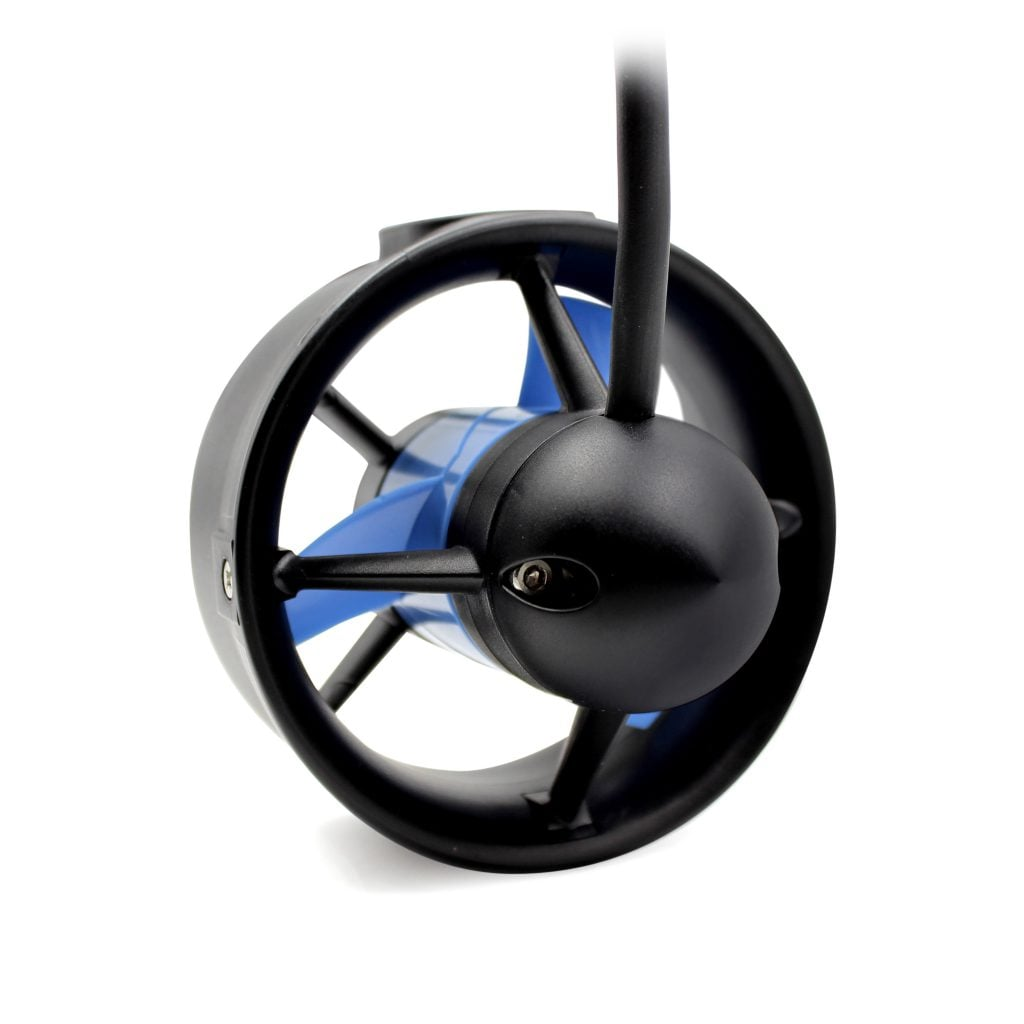
\includegraphics[height=2.3cm, keepaspectratio]{t200_thruster.png}\\
        \vspace{0.2em}
        \tech{T200 Thruster}\\
        \footnotesize\textbf{Standard ROV \& ASV}
      \end{center}
      \scriptsize
      \begin{itemize}
        \item Poussée : \textbf{$5.25\,\text{kgf}$}.
        \item Tension : $7\text{--}20\,\text{V}$ (4S).
        \item Moteur noyé, paliers PEEK.
        \item Référence BlueROV2 et BlueBoat (skid-steering).
      \end{itemize}
    \end{column}

    \begin{column}{0.32\textwidth}
      \begin{center}
        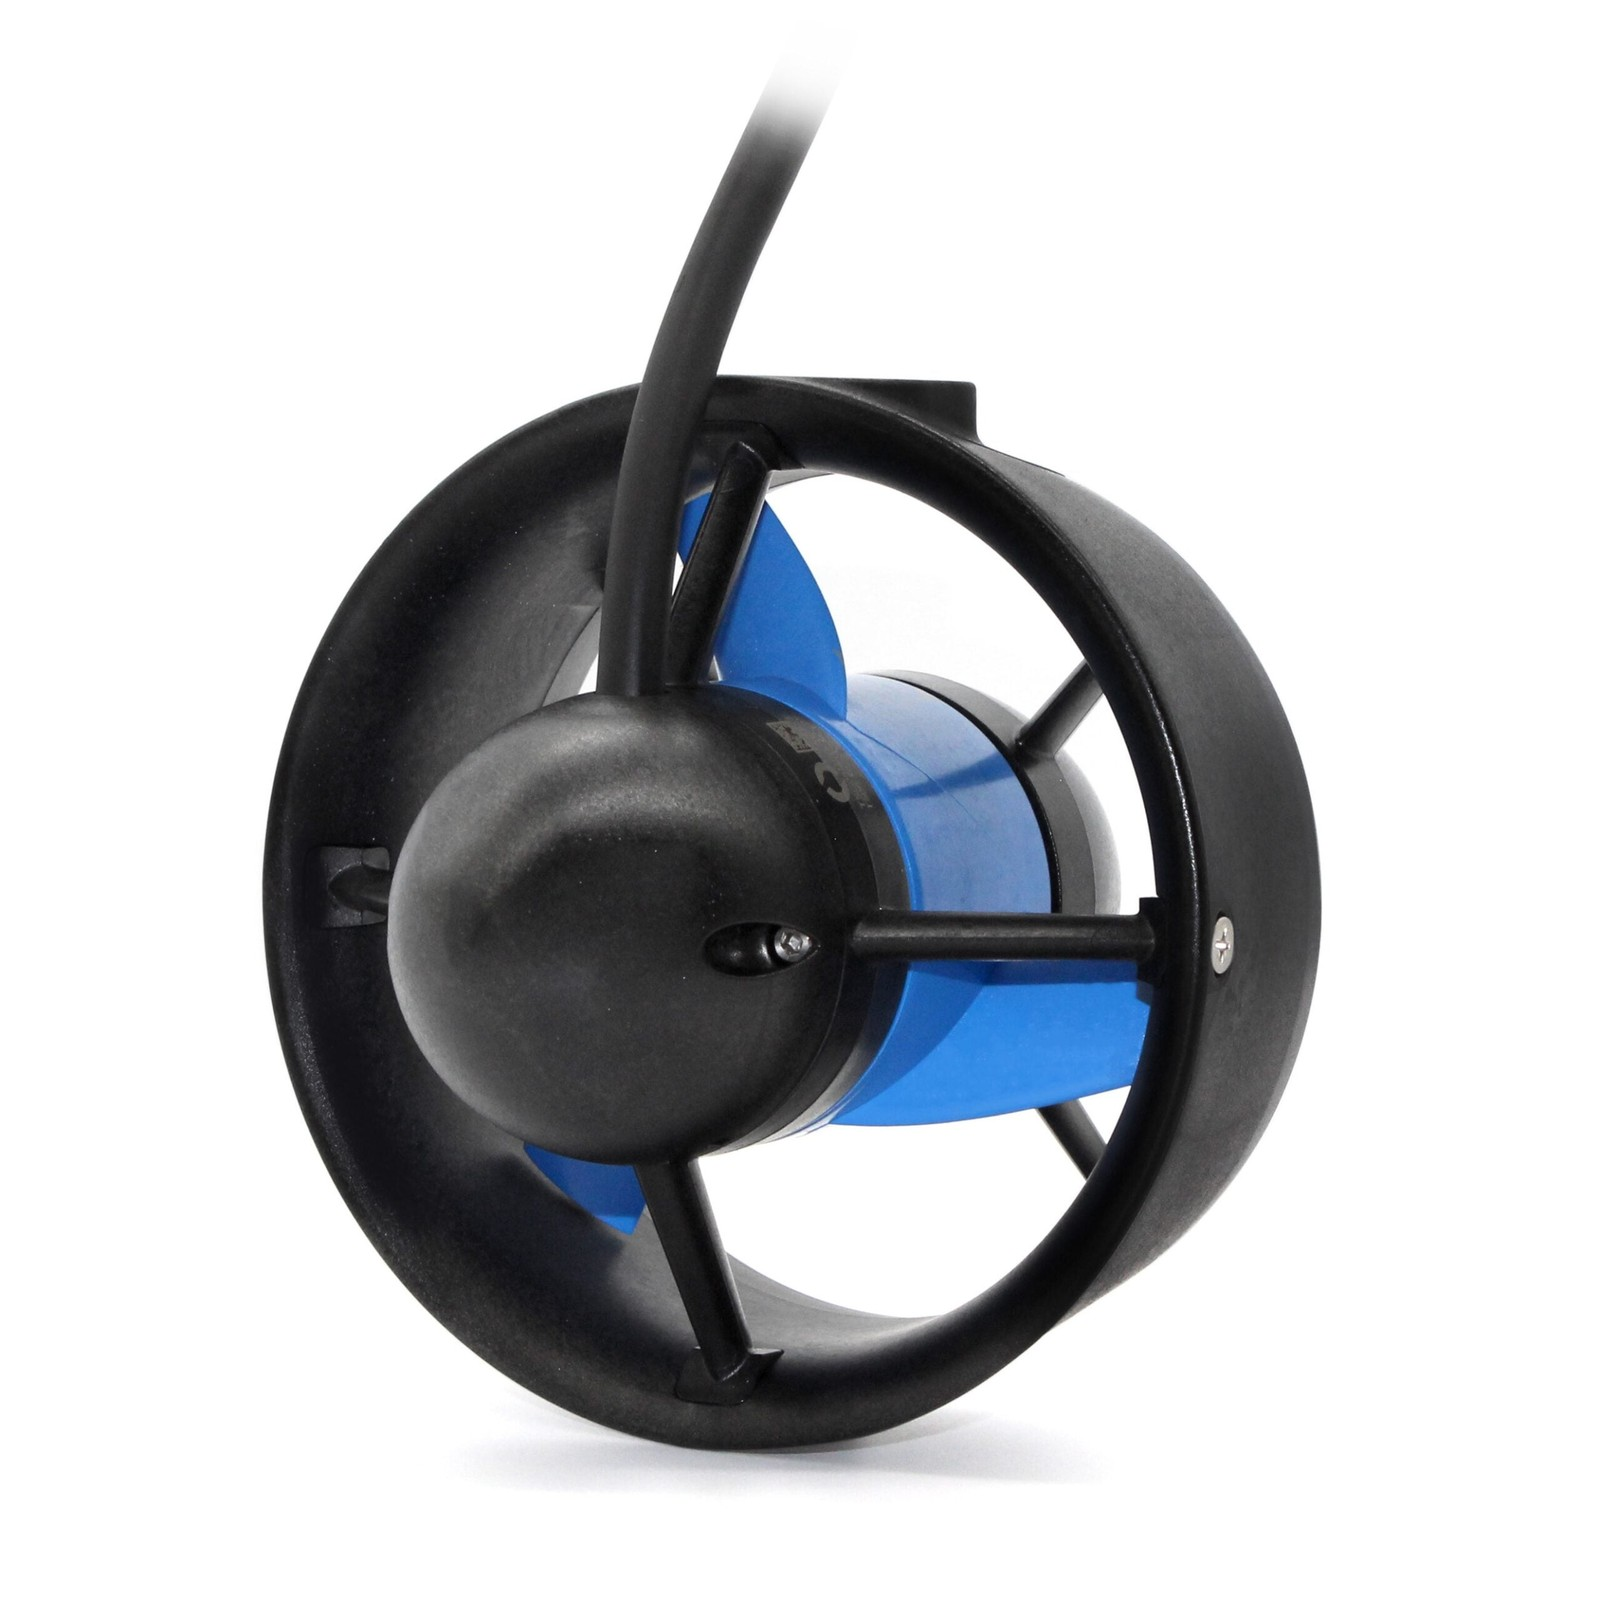
\includegraphics[height=2.3cm, keepaspectratio]{t500_thruster.jpg}\\
        \vspace{0.2em}
        \tech{T500 Thruster}\\
        \footnotesize\textbf{Haute Poussée ($3\times$ T200)}
      \end{center}
      \scriptsize
      \begin{itemize}
        \item Poussée : jusqu'à \succw{$\mathbf{16.1\,\text{kgf}}$} !
        \item Tension nominale : \textbf{$24\,\text{V}$}.
        \item Rendement accru.
        \item Pour gros AUVs, remorquage d'antennes et ASVs rapides.
      \end{itemize}
    \end{column}

    \begin{column}{0.32\textwidth}
      \begin{center}
        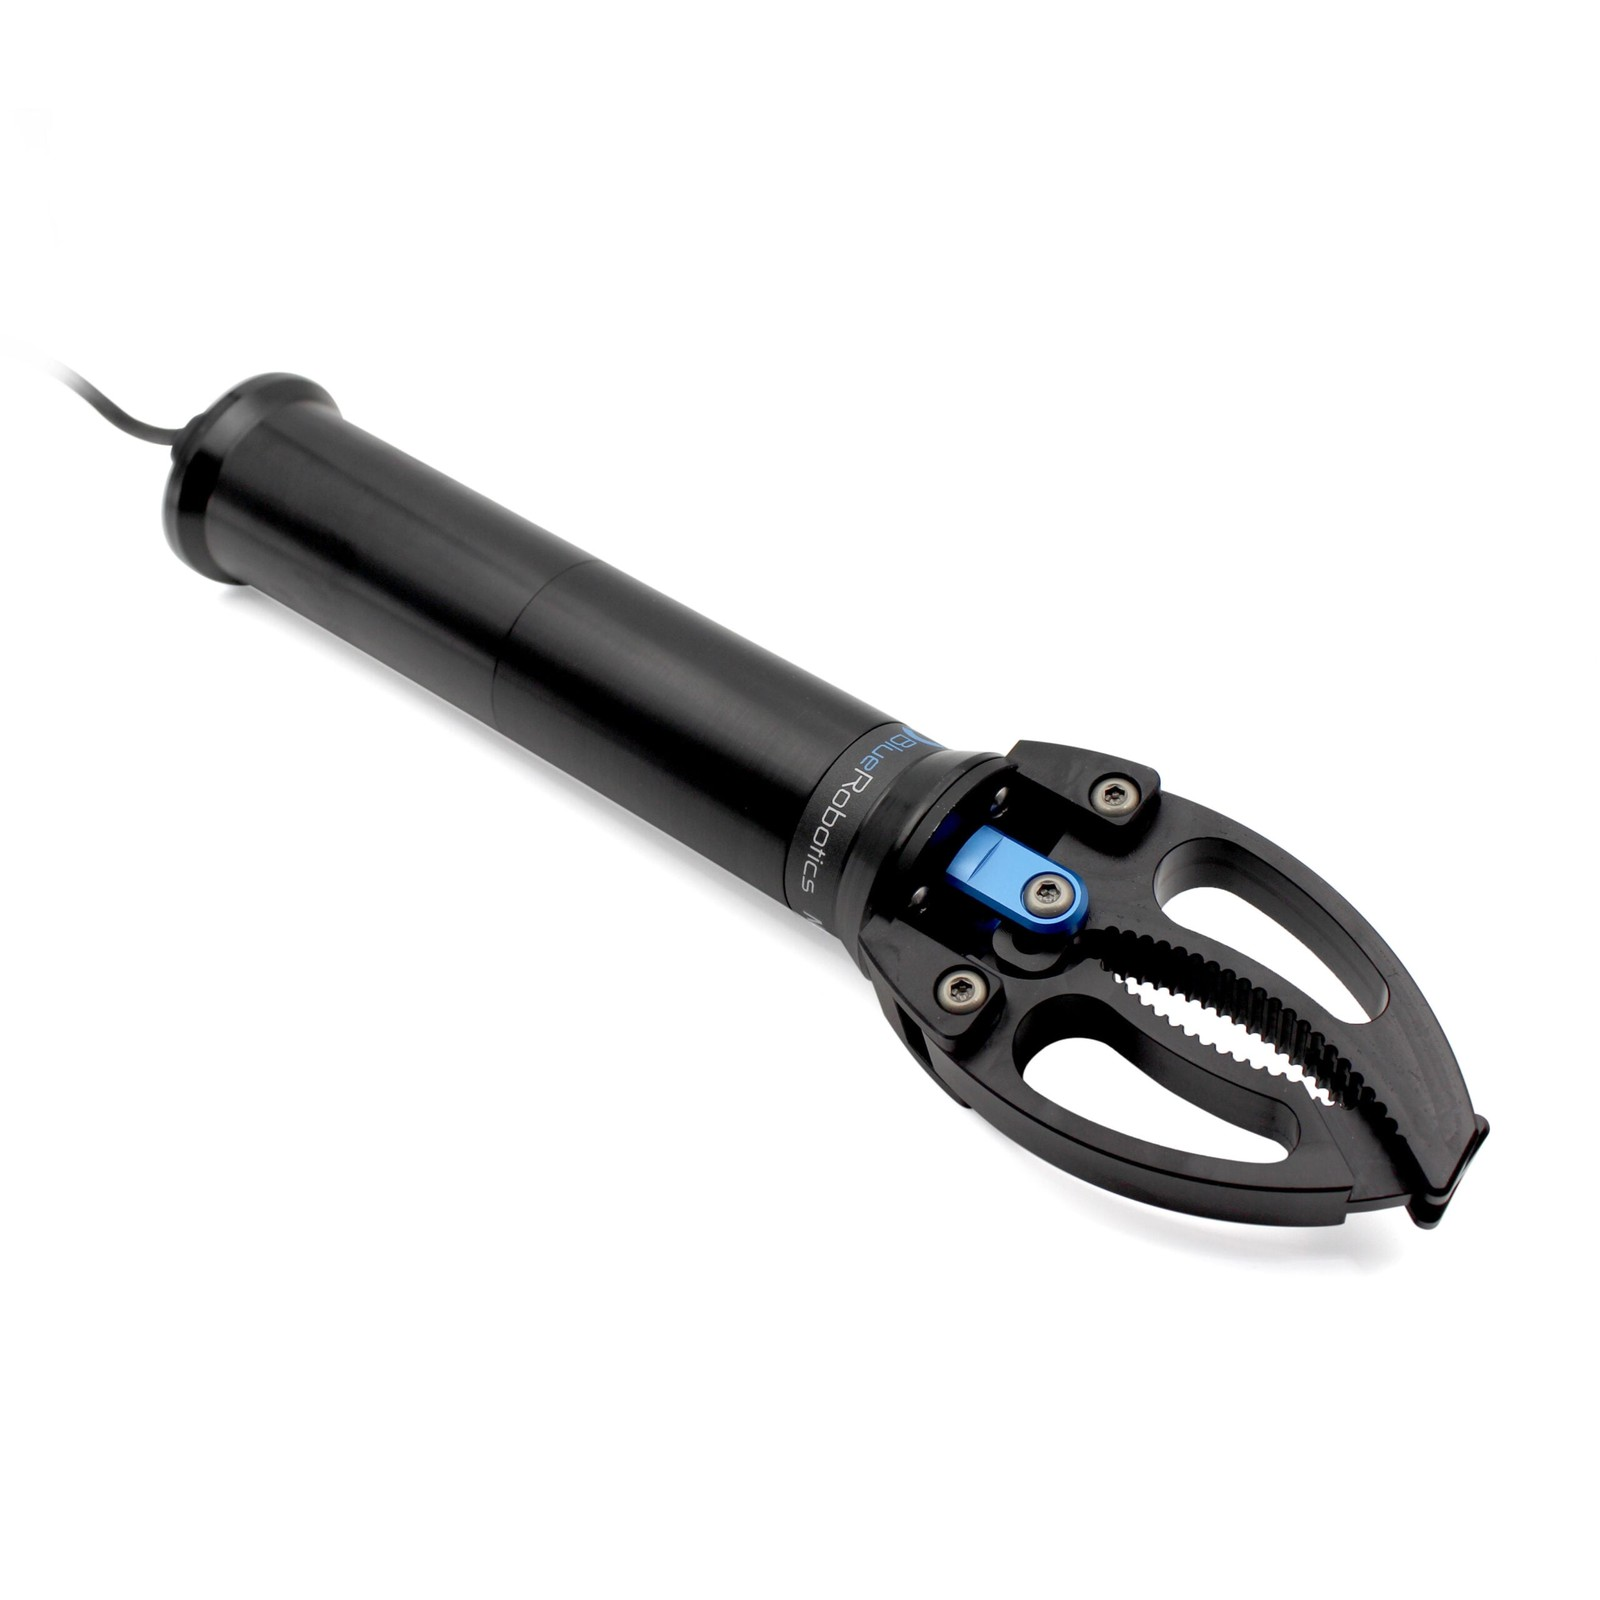
\includegraphics[height=2.3cm, keepaspectratio]{newton_gripper.jpg}\\
        \vspace{0.2em}
        \tech{Pince Newton \& Servos}\\
        \footnotesize\textbf{Actionneur Submersible 300m}
      \end{center}
      \scriptsize
      \begin{itemize}
        \item Commande servo PWM standard ($1.1\text{--}1.9\,\text{ms}$).
        \item Motoréducteur étanche + vis sans fin.
        \item Force de serrage : \textbf{$97\,\text{N}$}.
        \item Prélèvements d'échantillons et largage d'instruments.
      \end{itemize}
    \end{column}
  \end{columns}
\end{frame}

\begin{frame}{1.4 Les Calculateurs : Du Pixhawk à la Carte Navigator}
  \begin{columns}[T]
    \begin{column}{0.42\textwidth}
      \begin{center}
        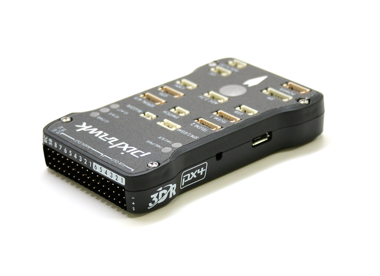
\includegraphics[height=2.2cm, keepaspectratio]{pixhawk_autopilot.png}\\
        \vspace{0.2em}
      \end{center}
      \scriptsize
      \begin{block}{\tech{L'Approche Historique : Pixhawk}}
        \begin{itemize}
          \item Autopilote standard hérité du drone aérien.
          \item Connecté au Raspberry Pi par câble USB/série externe.
          \item Vulnérabilité des connecteurs micro-USB dans les petits caissons étanches.
        \end{itemize}
      \end{block}
    \end{column}

    \begin{column}{0.56\textwidth}
      \begin{center}
        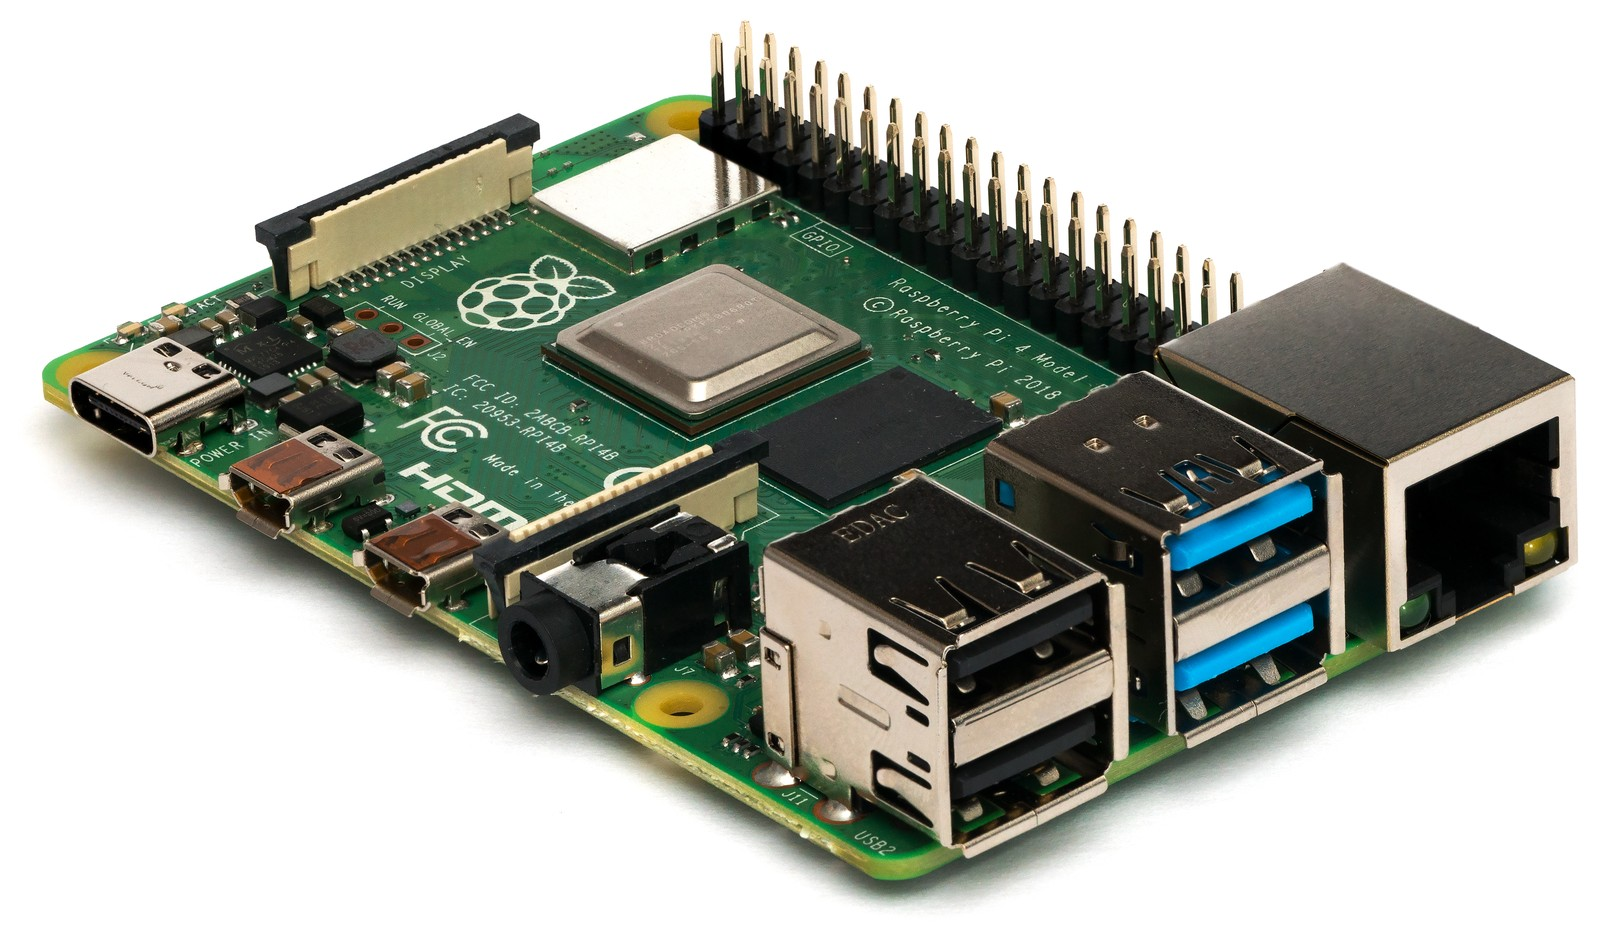
\includegraphics[height=2.0cm, keepaspectratio]{raspberry_pi_4.jpg}
        \hspace{0.3cm}
        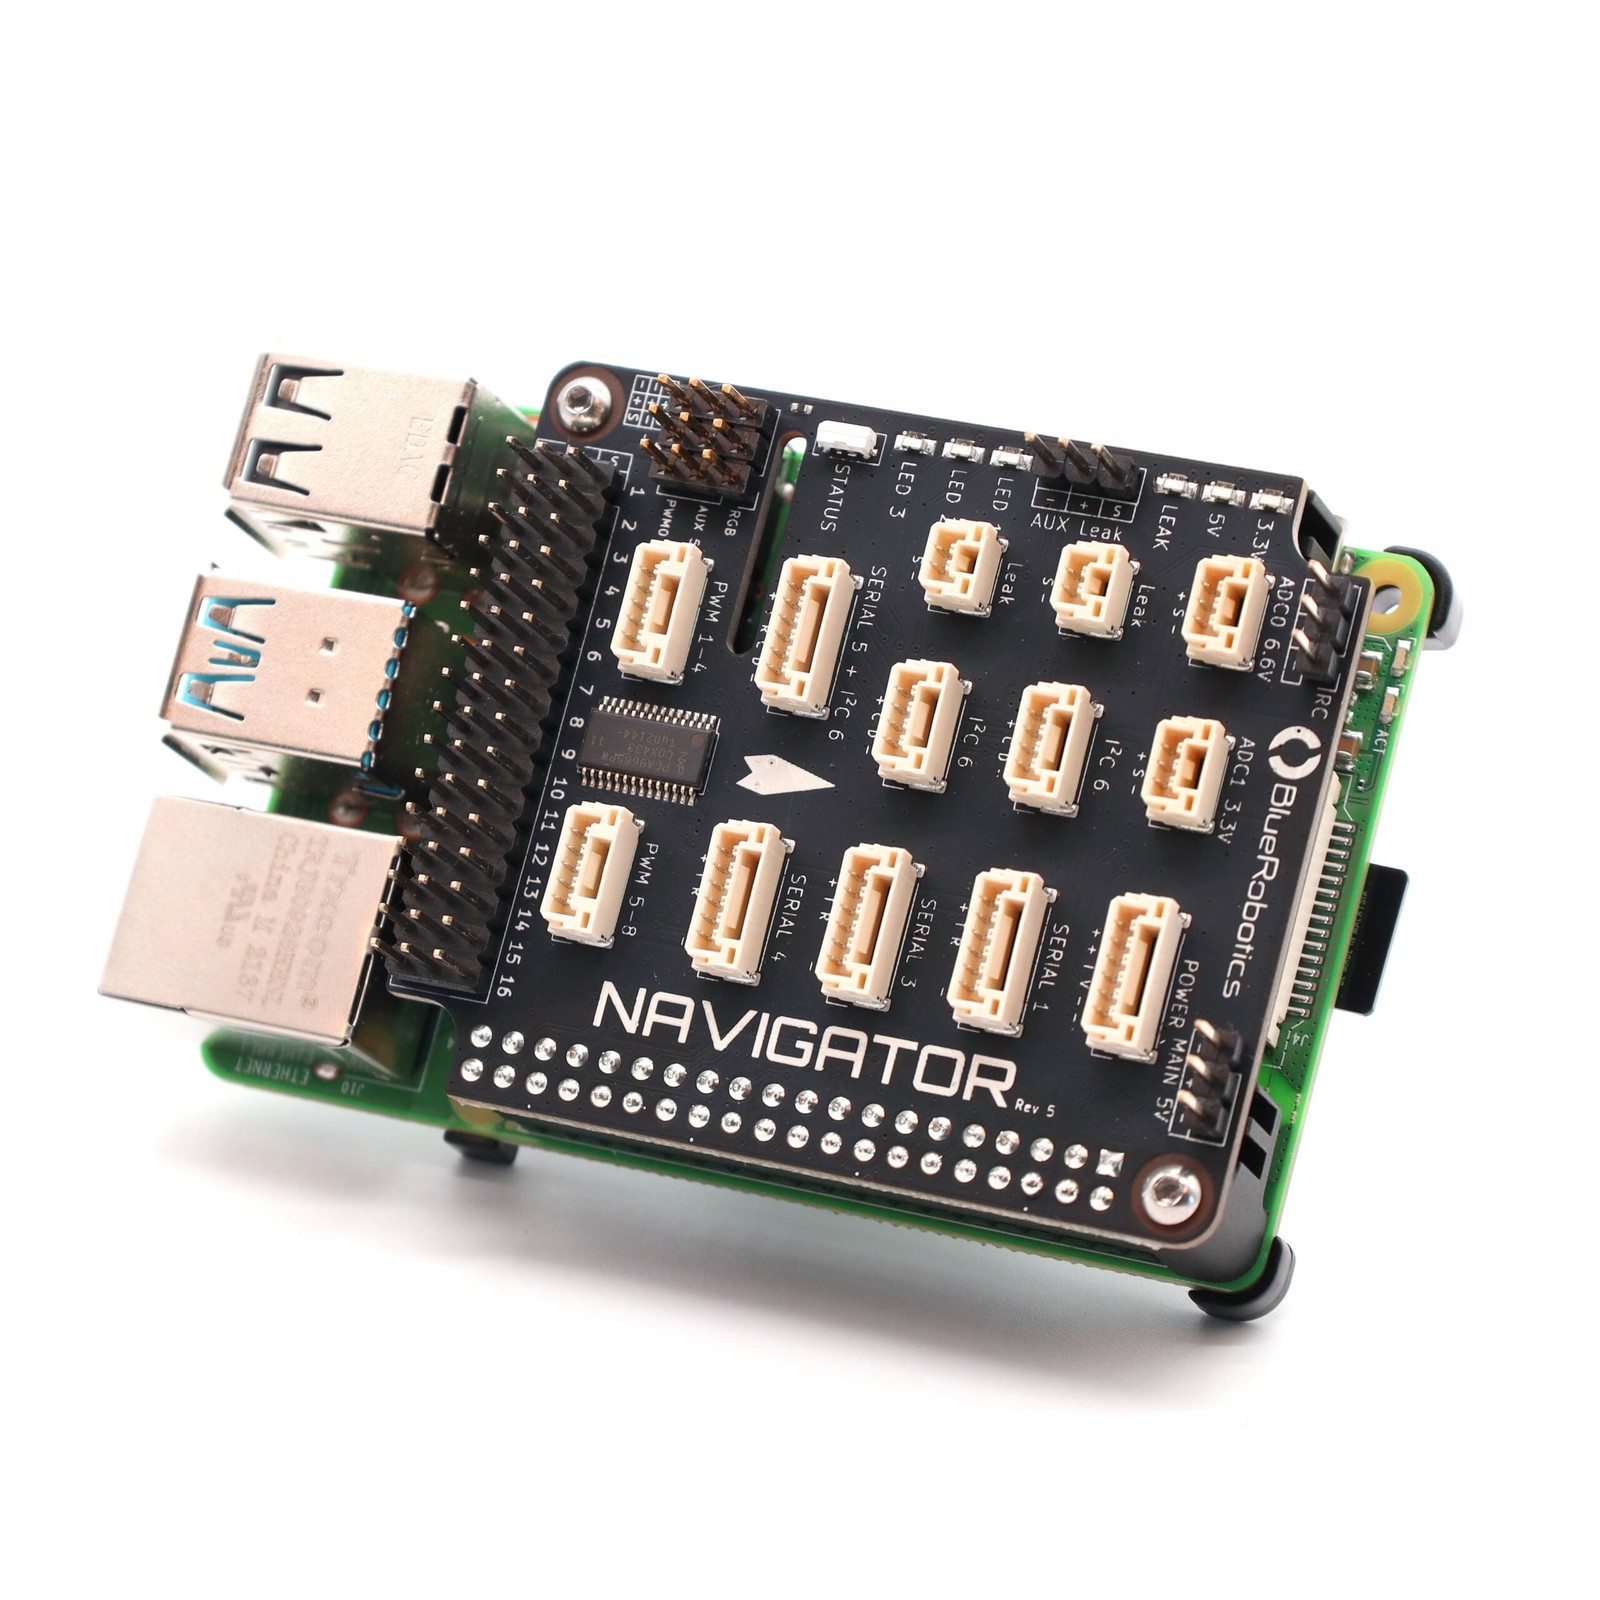
\includegraphics[height=2.0cm, keepaspectratio]{navigator_board.jpg}\\
        \vspace{0.2em}
      \end{center}
      \scriptsize
      \begin{exampleblock}{Le Tandem Moderne : Raspberry Pi 4 + Navigator}
        \begin{itemize}
          \item \textbf{HAT dédié} s'enfichant directement sur le GPIO du \textbf{Raspberry Pi 4 / 5}.
          \item \textbf{Capteurs intégrés} : double IMU redondante (ICM-20602 + ICM-20948), magnétomètre MMC5983MA, pression interne.
          \item \textbf{Connectique native} : 16 sorties PWM, bus I2C, ADC, ports séries (JST-GH).
          \item Une seule alimentation, zéro câble USB interne !
        \end{itemize}
      \end{exampleblock}
    \end{column}
  \end{columns}
\end{frame}

\begin{frame}{1.5 Mesure de Profondeur : Les Capteurs Bar30 et Bar02}
  \begin{center}
    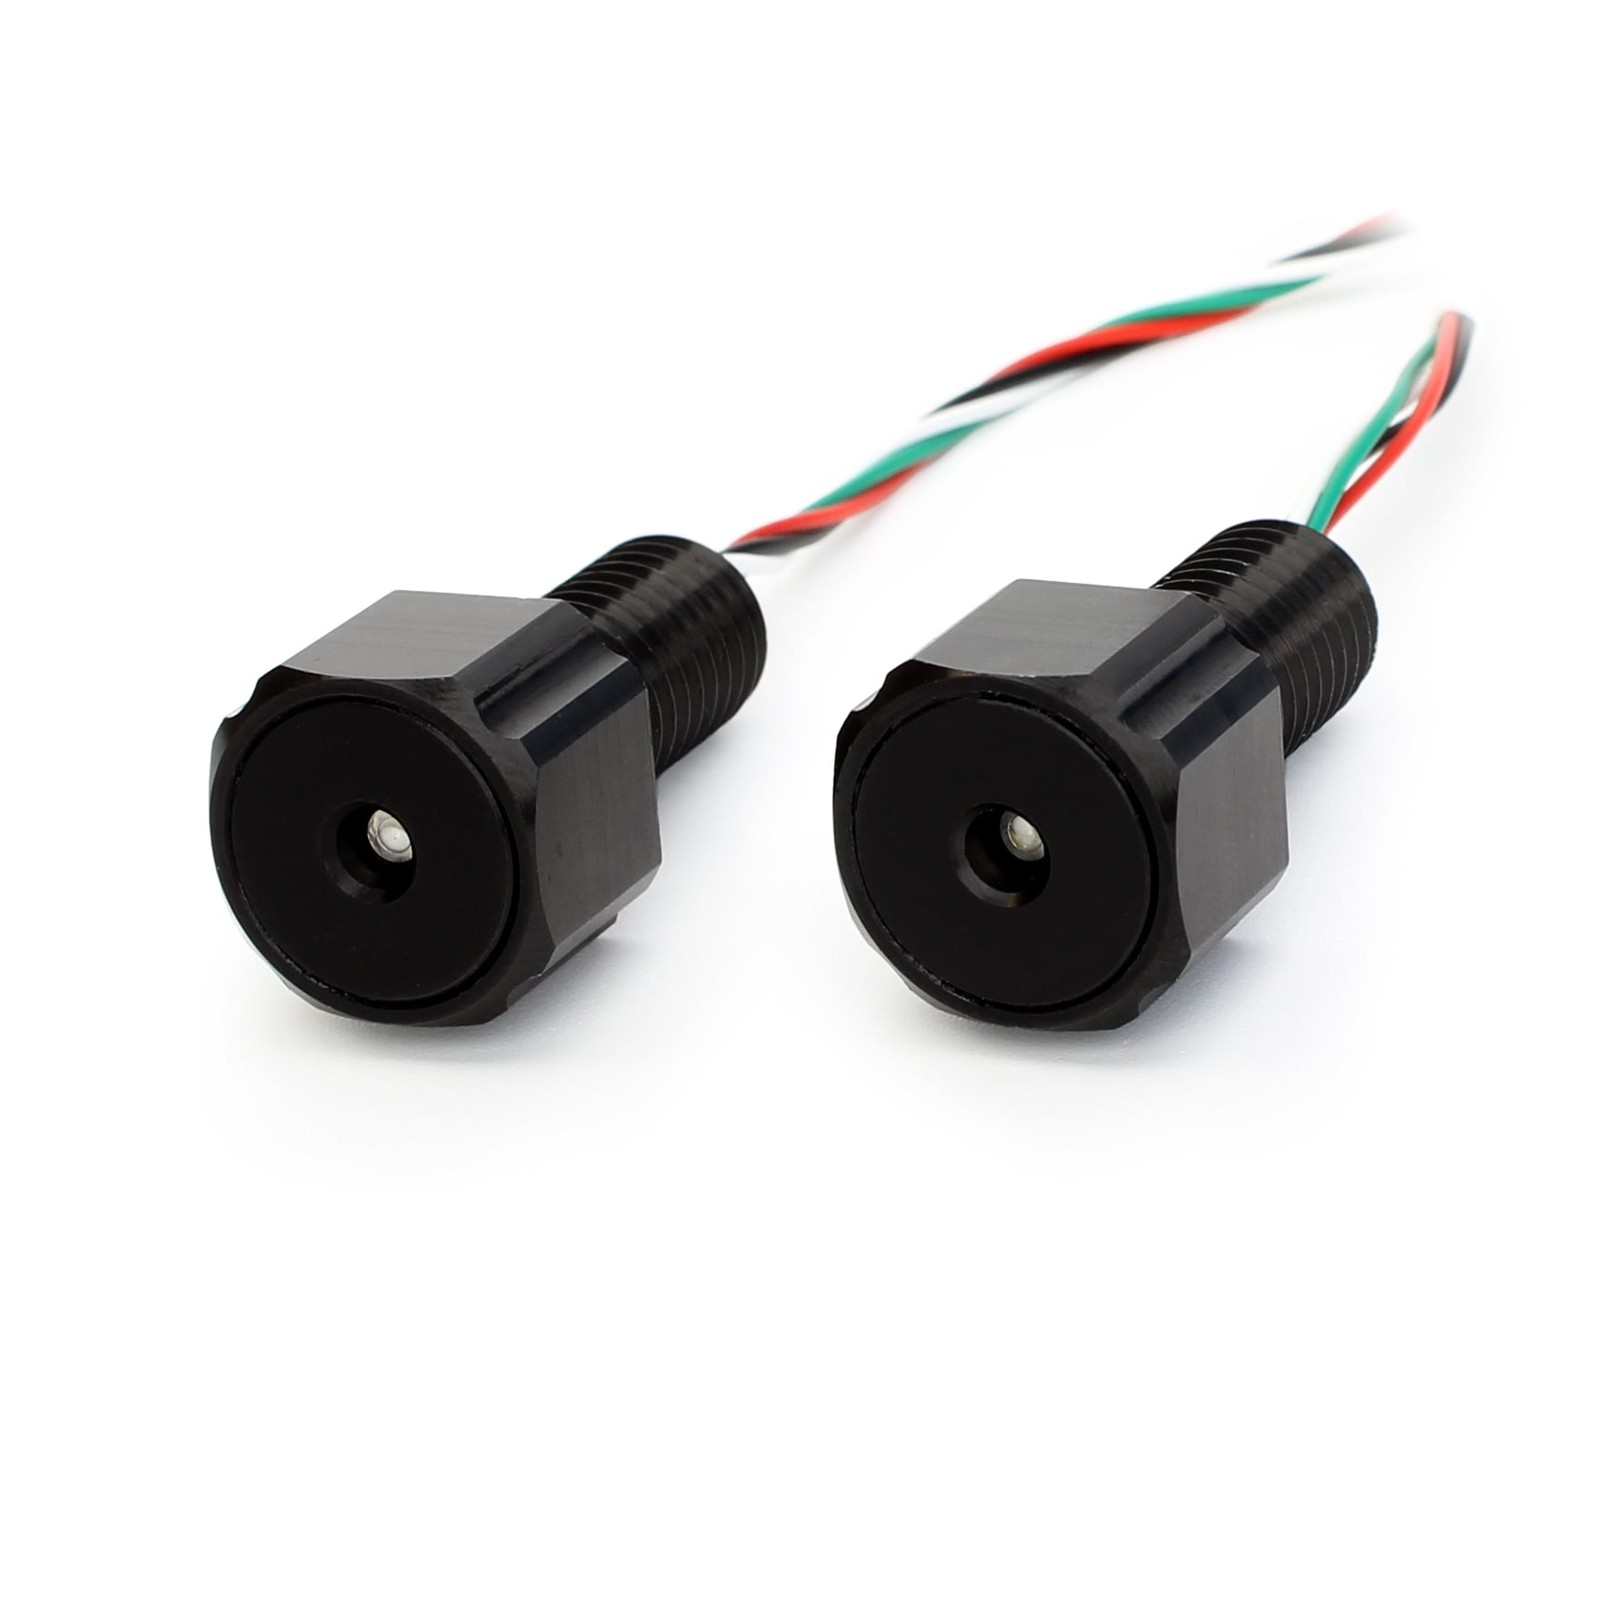
\includegraphics[trim=30 130 30 50, clip, height=2.3cm, keepaspectratio]{bar30_sensor.jpg}\\[0.2em]
    \footnotesize\tech{Boîtier M10 Étanche Commun (Bar30 \& Bar02)}\\
    \scriptsize\textcolor{DarkSlate!70}{Corps aluminium anodisé M10 étanche, joint torique, interface numérique bus I\textsuperscript{2}C (3.3\,V, adresse \code{0x76}).}
  \end{center}
  \vspace{-0.3em}
  \begin{columns}[T]
    \begin{column}{0.48\textwidth}
      \begin{block}{\tech{Capteur Bar30 (MS5837-30BA)}}
        \scriptsize
        \begin{itemize}
          \item \textbf{Gamme} : $0\text{--}30\,\text{bar}$ ($0\text{--}300\,\text{m}$ de profondeur).
          \item \textbf{Résolution} : \succw{$\mathbf{0.2\,\text{mm}}$ d'eau} ($0.16\,\text{mbar}$).
          \item \textbf{Usage cible} : ROVs \& AUVs côtiers (BlueROV2).
          \item \textbf{Contrôle} : Asservissement vertical fin (\textit{Depth Hold}).
          \item \textbf{Tarif indicatif} : \tech{$\approx 80\,\$$} (missions intermittentes).
        \end{itemize}
      \end{block}
    \end{column}
    \begin{column}{0.48\textwidth}
      \begin{block}{\tech{Capteur Bar02 (MS5837-02BA)}}
        \scriptsize
        \begin{itemize}
          \item \textbf{Gamme} : $0\text{--}2\,\text{bar}$ ($0\text{--}10\,\text{m}$ de profondeur / surface).
          \item \textbf{Résolution} : \succw{$<\mathbf{0.05\,\text{mm}}$ d'eau} (ultra-fine).
          \item \textbf{Technologie} : Silicium piézorésistif sous gel.
          \item \textbf{Usage cible} : Lacs, marégraphes, houle sur ASV.
          \item \textbf{Entretien} : Rinçage eau douce post-mission obligatoire.
        \end{itemize}
      \end{block}
    \end{column}
  \end{columns}
\end{frame}

\begin{frame}{1.5b Immersion Continue : Capteurs Haute Résistance BarXT}
  \begin{columns}[c]
    \begin{column}{0.44\textwidth}
      \begin{center}
        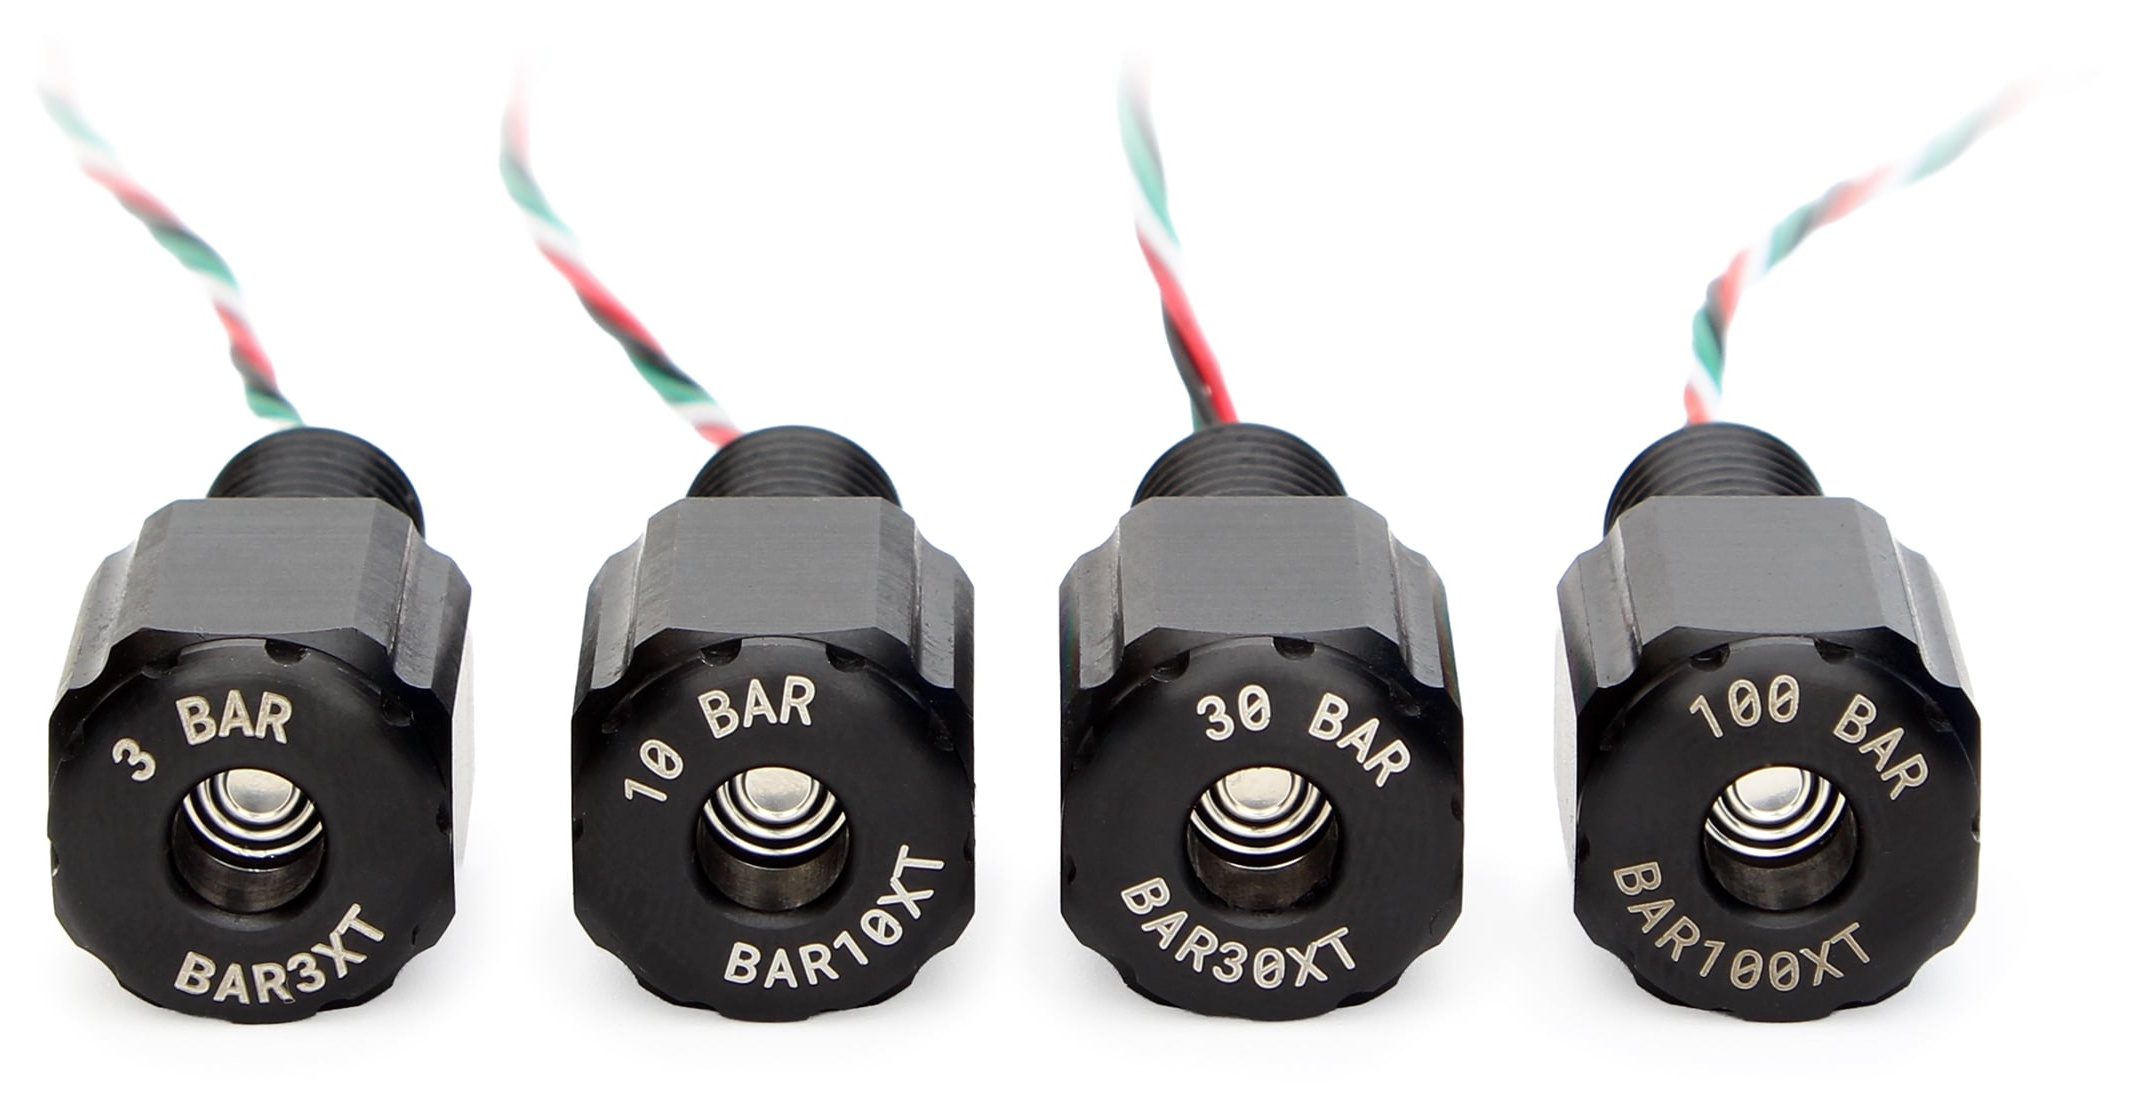
\includegraphics[height=1.65cm, keepaspectratio]{barxt_sensor_clean.jpg}\\[0.2em]
        \footnotesize\tech{Série Blue Robotics BarXT (\textit{Extended Submersion})}\\[0.1em]
        \scriptsize\textcolor{DarkSlate!70}{Corps Inox 316L oxyde noir, capteur soudé Keller 4LD, bus I\textsuperscript{2}C (\code{0x40}).}
      \end{center}
    \end{column}
    \begin{column}{0.54\textwidth}
      \begin{alertblock}{La Limite des Capteurs Standard ($\approx 80\,\$$)}
        \scriptsize
        \begin{itemize}
          \item \textbf{Gel silicone en contact} : colmatage par \textit{biofouling} et hydrolyse en immersion permanente.
          \item \textbf{Aluminium M10} : sensibilité à la corrosion galvanique.
          \item Rinçage eau douce et séchage obligatoires post-mission.
        \end{itemize}
      \end{alertblock}
    \end{column}
  \end{columns}

  \vspace{0.15em}

  \begin{columns}[T]
    \begin{column}{0.48\textwidth}
      \begin{block}{\tech{Atouts Technologiques BarXT}}
        \scriptsize
        \begin{itemize}
          \item \textbf{Immersion indéfinie} : conçu pour stations fond de mer, bouées \& mouillages scientifiques permanents.
          \item \textbf{Cellule Keller 4LD scellée} : membrane inox soudée, huile isolante, zéro gel exposé.
          \item \textbf{Protection mécanique} : capot frontal ajouré.
          \item \textbf{Gamme étendue} : de $3\,\text{bar}$ jusqu'à \succw{$100\,\text{bar}$ ($1000\,\text{m}$)}.
        \end{itemize}
      \end{block}
    \end{column}

    \begin{column}{0.48\textwidth}
      \begin{exampleblock}{Arbitrage Opérationnel : $80\,\$$ vs $380\,\$$}
        \scriptsize
        \begin{itemize}
          \item \textbf{Bar30 / Bar02 ($\approx 80\,\$$)} : parfait pour ROVs d'inspection, drones de surface, plongées courtes.
          \item \textbf{Série BarXT ($\approx 380\,\$$)} : facteur \alertw{$\approx 4.7\times$} de surcoût à l'achat.
          \item \textbf{Rentabilité terrain} : le delta de $\sim 300\,\$$ est négligeable face au coût d'une campagne navale pour remplacer un capteur dérivé ou colmaté.
        \end{itemize}
      \end{exampleblock}
    \end{column}
  \end{columns}
\end{frame}

\begin{frame}{1.6 Les Autopilotes Open-Source : ArduSub vs ArduRover vs PX4}
  \begin{table}[h]
    \centering
    \small
    \begin{tabularx}{\textwidth}{l p{3.2cm} p{3.2cm} X}
      \toprule
      \textbf{Autopilote} & \textbf{Vecteur Cible} & \textbf{Modes Clés} & \textbf{Intérêt Scientifique} \\
      \midrule
      \tech{ArduSub} & ROVs \& AUVs subaquatiques & Stabilize, \textbf{Depth Hold}, Auto, PosHold (DVL) & Asservissement vertical fin via Bar30, gestion de 6 à 8 thrusters vectoriels. \\
      \rowcolor{OceanGray}
      \tech{ArduRover} & ASV / Drones de surface (\textbf{BlueBoat}) & Manual, Acro, \textbf{Auto Survey}, RTL & Navigation différentielle (*skid-steering*), quadrillage bathymétrique par GPS. \\
      \tech{PX4} & Aérien / sous-marin expérimental & Offboard, Position, Mission & Architecture orientée micro-services, pont micro-ROS / uORB natif. \\
      \bottomrule
    \end{tabularx}
  \end{table}

  \begin{block}{Le Protocole MAVLink : La Passerelle Universelle}
    Toutes les données de vol (attitude, tension batterie, profondeur Bar30, alertes fuite) sont encapsulées dans des paquets \textbf{MAVLink} légers, standardisés et lisibles par n'importe quel langage (Python via \code{pymavlink}, C++, ROS via \code{mavros}).
  \end{block}
\end{frame}

\begin{frame}{1.7 Cadre Réglementaire Français : Le Statut du Drone Maritime}
  \begin{columns}[T]
    \begin{column}{0.49\textwidth}
      \begin{block}{\tech{Textes Fondateurs en Droit Français}}
        \scriptsize
        \begin{itemize}
          \item \href{https://www.legifrance.gouv.fr/jorf/id/JORFTEXT000044202140}{\underline{\textbf{Ordonnance n° 2021-1330}}} (13 oct. 2021) : statut des navires autonomes et drones.
          \item \href{https://www.legifrance.gouv.fr/jorf/id/JORFTEXT000049583905}{\underline{\alertw{Décret n° 2024-461}}} (22 mai 2024) : exploitation, sécurité et formation.
          \item \textbf{Code des transports} :
            \begin{itemize}\scriptsize
              \item \href{https://www.legifrance.gouv.fr/codes/article_lc/LEGIARTI000049585210}{\underline{\tech{Art. R. 5000-1}}} : Définition légale stricte.
              \item \href{https://www.legifrance.gouv.fr/codes/article_lc/LEGIARTI000049585847}{\underline{\tech{Art. R. 5241-2}}} : Navigation subaquatique.
              \item \href{https://www.legifrance.gouv.fr/codes/article_lc/LEGIARTI000049586745}{\underline{\tech{Art. R. 5271-1}}} : Titres et qualifications.
            \end{itemize}
        \end{itemize}
      \end{block}

      \vspace{-0.3em}
      \begin{block}{\succw{Obligation du Brevet Capitaine 200}}
        \scriptsize
        La recherche en mer relève du \textbf{secteur professionnel}. La responsabilité légale nautique et le respect du RIPAM (COLREG 72) imposent la présence ou supervision d'un marin breveté \alertw{Capitaine 200} (Marine Marchande) sur le navire support ou au centre de télé-opération (COD).
      \end{block}
    \end{column}

    \begin{column}{0.49\textwidth}
      \begin{alertblock}{Critères Cumulatifs Drone Maritime (\code{Art. R. 5000-1})}
        \scriptsize
        Engin flottant de surface ou sous-marin opéré à distance / autonome sans personne à bord :
        \begin{itemize}\scriptsize
          \item \textbf{Longueur hors-tout} : $1\,\text{m} < L_{\text{HT}} < 16\,\text{m}$.
          \item \textbf{Vitesse maximale} : $\le 20\,\text{n\oe uds}$ ($\approx 37\,\text{km/h}$).
          \item \textbf{Énergie cinétique} : $< 300\,\text{kJ}$ ($\frac{1}{2} M V_{\max}^2$).
          \item \textbf{Jauge brute} : $< 100$.
        \end{itemize}
      \end{alertblock}

      \vspace{-0.3em}
      \begin{exampleblock}{Exclusions Expresses (\code{Art. R. 5000-1})}
        \scriptsize
        \begin{itemize}\scriptsize
          \item \textbf{Micro-engins} : longueur $\le 1.00\,\text{m}$.
          \item \textbf{Bande des 300 mètres} : engins radiocommandés sous police du maire.
          \item \textbf{Objets non man{\oe}uvrants} : bouées et gliders dérivants.
        \end{itemize}
      \end{exampleblock}
    \end{column}
  \end{columns}
\end{frame}

\begin{frame}{1.7b Déploiement Scientifique : Astuces Légales \& Contournements}
  \begin{columns}[T]
    \begin{column}{0.49\textwidth}
      \begin{block}{\tech{3 Leviers pour Alléger les Contraintes}}
        \scriptsize
        \begin{itemize}
          \item \textbf{1. Le ROV filaire (BlueROV2)} : relié en permanence par ombilical. Qualifié d'\textbf{équipement captif immergé} sous la garde du bateau/quai $\rightarrow$ \succw{zéro qualification drone requise} !
          \item \textbf{2. Le seuil des $\le 1\,\text{m}$ (Micro-AUV)} : l'\href{https://www.legifrance.gouv.fr/codes/article_lc/LEGIARTI000049585210}{\underline{\code{Art. R. 5000-1}}} impose $L > 1\,\text{m}$. Un engin $\le 1\,\text{m}$ \succw{échappe à la qualification de drone maritime} (modélisme naval / outil scientifique léger).
          \item \textbf{3. Bande des 300 m \& Eaux intérieures} : à vue à $<300\,\text{m}$ du rivage (police du maire, autorisations simples) ou en lacs/fleuves (régime VNF / DDTM).
        \end{itemize}
      \end{block}
    \end{column}

    \begin{column}{0.49\textwidth}
      \begin{alertblock}{4. Navire Support avec Capitaine 200}
        \scriptsize
        En mer ouverte avec un ASV $>1\,\text{m}$ (BlueBoat) ou AUV :
        \begin{itemize}\scriptsize
          \item Naviguer avec un semi-rigide d'escorte à vue immédiate.
          \item \alertw{Embarquer un marin Capitaine 200} (agent breveté du labo, skipper station marine CNRS ou prestataire).
          \item Le Capitaine 200 assure la veille optique 360°, la liaison VHF 16 avec le CROSS et la responsabilité RIPAM.
        \end{itemize}
      \end{alertblock}

      \vspace{-0.3em}
      \begin{exampleblock}{5. Déclaration Prémar \& AVURNAV}
        \scriptsize
        Déclaration d'expérimentation DML / Préfecture Maritime : publication d'un \textbf{AVURNAV} temporaire réservant la zone aux navigateurs tiers.
      \end{exampleblock}
    \end{column}
  \end{columns}
\end{frame}

\begin{frame}{1.7c Sécuriser sa Zone : La Plateforme PING (Shom / DGAMPA)}
  \begin{columns}[T]
    \begin{column}{0.52\textwidth}
      \begin{block}{\tech{Qu'est-ce que la Plateforme PING ?}}
        \scriptsize
        \begin{itemize}
          \item \textbf{P}lateforme d'\textbf{I}nformation \textbf{N}autique \textbf{G}éoréférencée : portail officiel développé conjointement par le \textbf{Shom} et la \textbf{DGAMPA}.
          \item Accessible en ligne : \href{https://portail.ping-info-nautique.fr/}{\underline{\tech{portail.ping-info-nautique.fr}}}
          \item Également intégrée dans l'application mobile \textbf{Nav\&Co} (Shom / Office Français de la Biodiversité).
          \item Outil de référence pour la sécurité maritime en France (Manche, Atlantique, Méditerranée, Outre-mer).
        \end{itemize}
      \end{block}

      \begin{alertblock}{Le Réflexe Avant Toute Mise à l'Eau}
        \scriptsize
        Consulter PING le matin même de la manip : un polygone de tir temporaire non anticipé peut entraîner l'interception de votre drone par les vedettes de la Marine ou des Affaires Maritimes.
      \end{alertblock}
    \end{column}

    \begin{column}{0.46\textwidth}
      \begin{exampleblock}{Informations Clés Diffusées sur PING}
        \scriptsize
        \begin{itemize}
          \item \textbf{Avis aux Navigateurs} : cartographie spatialisée des \alertw{AVURNAV} (urgents) et \textbf{AVINAV} (locaux).
          \item \textbf{Zones d'Exclusion Militaires} : polygones de tir réel, essais sous-marins et torpillages.
          \item \textbf{Couloirs de Navigation} : Dispositifs de Séparation de Trafic (DST) et chenaux d'accès aux ports.
          \item \textbf{Restrictions Environnementales} : cantonnements, réserves naturelles, arrêtés préfectoraux de mouillage (ex: Posidonie).
          \item \textbf{Infrastructures Sous-Marines} : câbles télécoms, émissaires et épaves.
        \end{itemize}
      \end{exampleblock}
    \end{column}
  \end{columns}
\end{frame}

\begin{frame}{Synthèse du Module 1 : Briques Matérielles \& Cadre Opérationnel}
  \begin{exampleblock}{La recette gagnante pour un drone scientifique opérationnel}
    \begin{enumerate}
      \item \textbf{Base mécanique éprouvée} : coque ouverte modulaire (BlueROV2 ou BlueBoat).
      \item \textbf{Motorisation robuste} : propulseurs T200 étanches par conception et ESCs réversibles.
      \item \textbf{C{\oe}ur numérique intégré} : couple Raspberry Pi 4 + Navigator (Linux + temps réel).
      \item \textbf{Capteur environnemental clé} : capteur de pression Bar30 (résolution millimétrique).
      \item \textbf{Logiciel pérenne} : ArduSub ou ArduRover pour l'asservissement fiable en boucle fermée.
      \item \textbf{Cadrage réglementaire} : consultation de PING et choix du cadre (ROV captif, $\le 1\,\text{m}$ ou Capitaine 200).
    \end{enumerate}
  \end{exampleblock}

  \begin{alertblock}{La prochaine étape : L'étanchéité et le passage de câbles}
    Comment assembler ces composants pour qu'ils résistent à la pression sans couler ? Rendez-vous au Module 2 avec les caissons 4 pouces, les pénétrateurs WetLink, les connecteurs étanches Cobalt/SubConn et le BlueBoat !
  \end{alertblock}
\end{frame}

% ==============================================================================
% 02_differences_milieu.tex - Module 2 (10h30 - 12h00)
% Présentation d'un drone sous-marin : différences avec le drone aérien
% Fabrication réelle : Enceintes 3"/4", Pénétrateurs WetLink, Connecteurs Cobalt & SubConn, Test de vide, BlueBoat, DVL-A50
% ==============================================================================

\section{Module 2 : Différences avec l'Aérien \& Spécificités du Milieu}

\begin{frame}{2.1 Deux Mondes Physiques Opposés}
  \begin{table}[h]
    \centering
    \small
    \begin{tabularx}{\textwidth}{l X X}
      \toprule
      \textbf{Caractéristique} & \textbf{Milieu Aérien (UAV)} & \textbf{Milieu Marin (AUV / ROV)} \\
      \midrule
      \textbf{Masse volumique $\rho$} & $\approx 1.2\,\text{kg/m}^3$ & $\approx 1025\,\text{kg/m}^3$ \alertw{($\times 850$)} \\
      \textbf{Génération de force} & Portance aérodynamique ($v^2$) & Poussée d'Archimède statique \\
      \textbf{Stabilité naturelle} & Instable actif (quadrotor) & \succw{Stabilité statique passive ($B$ sur $G$)} \\
      \textbf{Pression ambiante} & $\approx 1\,\text{bar}$ (décroît) & $+1\,\text{bar}$ tous les $10\,\text{m}$ \\
      \textbf{Ondes radio / GNSS} & Propagation libre (GPS, 4G, WiFi) & \alertw{Absorption totale en qqs cm} \\
      \textbf{Visibilité / Optique} & Kilométrique & Métrique ($1\text{--}15\,\text{m}$), turbidité \\
      \textbf{Agression chimique} & Faible & Corrosion saline, conductivité \\
      \bottomrule
    \end{tabularx}
  \end{table}
\end{frame}

\begin{frame}{2.2 Hydrostatique : Flottabilité et Stabilité Passive}
  \begin{columns}[c]
    \begin{column}{0.44\textwidth}
      \begin{center}
        \begin{tikzpicture}[scale=0.82]
          % Corps de drone sous-marin
          \draw[thick, fill=OceanMedium!10, rounded corners=10pt] (-1.5,-1.3) rectangle (1.5,1.3);
          
          % Centre de carène B (haut)
          \coordinate (B) at (0, 0.65);
          \fill[OceanCyan] (B) circle (3.5pt);
          \draw[->, line width=1.8pt, OceanCyan] (B) -- (0, 1.85) node[above] {\small Poussée d'Archimède $\vec{F}_B$};
          \node[right=3pt of B] {\footnotesize \textbf{Centre de Carène $B$}};

          % Centre de gravité G (bas)
          \coordinate (G) at (0, -0.65);
          \fill[OceanDeep] (G) circle (3.5pt);
          \draw[->, line width=1.8pt, OceanCoral] (G) -- (0, -1.85) node[below] {\small Poids $\vec{P} = m\vec{g}$};
          \node[right=3pt of G] {\footnotesize \textbf{Centre de Gravité $G$}};

          % Bras de levier BG
          \draw[<->, thick, dashed] (-0.3,-0.6) -- (-0.3,0.6) node[midway, left] {\small $\overline{BG} > 0$};
        \end{tikzpicture}
      \end{center}
    \end{column}

    \begin{column}{0.54\textwidth}
      \small
      \textbf{Règle d'or de l'ingénierie sous-marine} :
      \begin{itemize}\setlength{\itemsep}{2pt}\setlength{\parskip}{0pt}
        \item Masses lourdes (batteries, caisson bas) \textbf{en bas}.
        \item Mousses flottantes (PEHD / syntactique) \textbf{en haut}.
        \item Couple de rappel hydrostatique :
        \begin{equation*}
          \setlength{\abovedisplayskip}{2pt}
          \setlength{\belowdisplayskip}{2pt}
          C_{\text{rappel}} = m \cdot g \cdot \overline{BG} \cdot \sin(\theta)
        \end{equation*}
        \item Drone \tech{auto-redressant} en roulis ($\phi$) et tangage ($\theta$) : zéro énergie dépensée pour rester horizontal !
      \end{itemize}

      \vspace{0.2em}
      \begin{block}{Flottabilité Positive de Sécurité}
        Lestage réglé pour $+200$ à $+500\,\text{g}$ nets : en cas de coupure de batterie, le robot \succw{remonte seul en surface}.
      \end{block}
    \end{column}
  \end{columns}
\end{frame}

\begin{frame}{2.3 Conception Réelle des Caissons Étanches (Modulaire 2" à 8")}
  \begin{columns}[c]
    \begin{column}{0.56\textwidth}
      \begin{block}{\tech{Gamme de Diamètres (2" à 8") \& Matériaux}}
        \scriptsize
        \begin{itemize}
          \item \textbf{Diamètres modulaires} : du \textbf{2"} (capteurs/éclairages), \textbf{3"} (batteries) et \textbf{4"} (électronique) jusqu'au \textbf{6"} et \textbf{8"} (gros payloads / AUV / baies de puissance).
          \item \textbf{Acrylique (PMMA)} : transparent, vue caméra \& voyants ($100\text{--}150\,\text{m}$).
          \item \textbf{Alu 6061-T6 anodisé dur} : certifié \succw{$\mathbf{400\text{--}500\,\text{m}}$}, dissipation thermique active des ESC / processeurs.
        \end{itemize}
      \end{block}

      \begin{block}{\succw{Flasques, Bouchons \& Verrouillage}}
        \scriptsize
        \begin{itemize}
          \item \textbf{Types d'embouts} : dômes optiques hémisphériques (caméras), flasques plates alu/acrylique (aveugles ou pré-percées 4 à 18 trous M10/M14).
          \item \textbf{Systèmes de fermetures} : cordon de verrouillage (*Locking Cord*) sans vis traversantes ou brides boulonnées.
          \item \textbf{Étanchéité} : double joint torique (*O-ring* radial + facial).
        \end{itemize}
      \end{block}
    \end{column}

    \begin{column}{0.42\textwidth}
      \begin{center}
        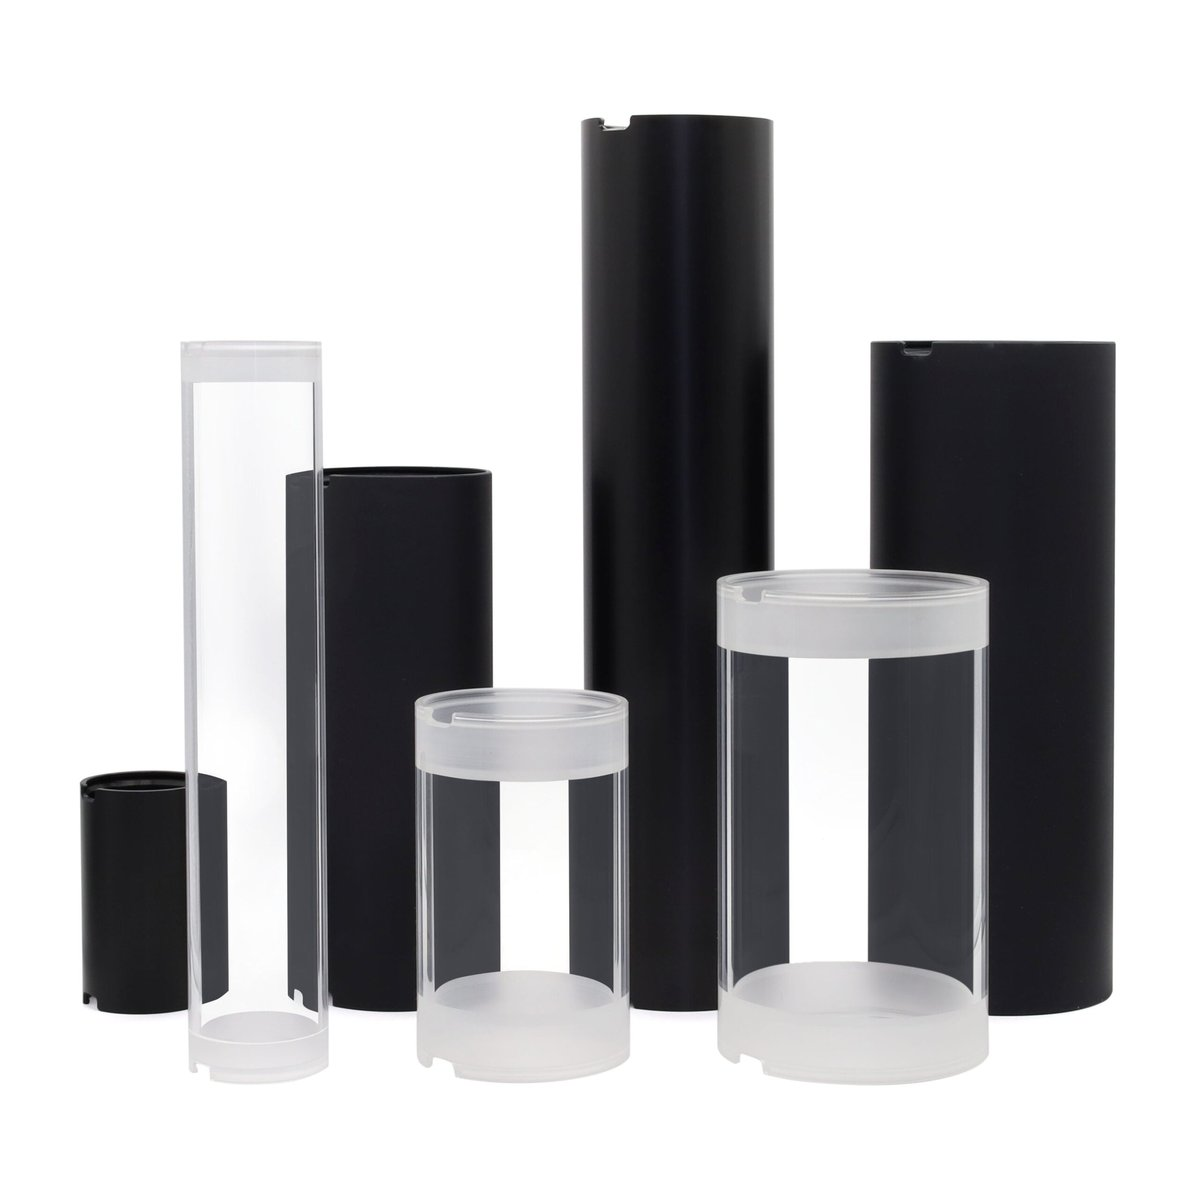
\includegraphics[width=\textwidth, height=3.6cm, keepaspectratio]{watertight_enclosure.jpg}\\
        \vspace{0.2em}
        \footnotesize\textbf{Caisson Étanche Modulaire (ex. 4")}\\
        \scriptsize\textit{Tube alu/acrylique, flasques O-ring, locking cord \& dôme optique}
      \end{center}
    \end{column}
  \end{columns}
\end{frame}

\begin{frame}{2.4 Franchissement de Paroi : WetLink Standard vs Nouveau JPT}
  \begin{block}{\succw{Révolution WetLink : La Fin Définitive du Potting Époxy}}
    \scriptsize
    L'ancienne coulée de résine époxy prenait 24h et était irréversible. Les pénétrateurs brevetés WetLink s'assemblent en \succw{\textbf{30 secondes}}, sans colle, et restent \succw{\textbf{100\% réutilisables}} en maintenance.
  \end{block}

  \vspace{-0.3em}
  \begin{columns}[T]
    \begin{column}{0.48\textwidth}
      \begin{center}
        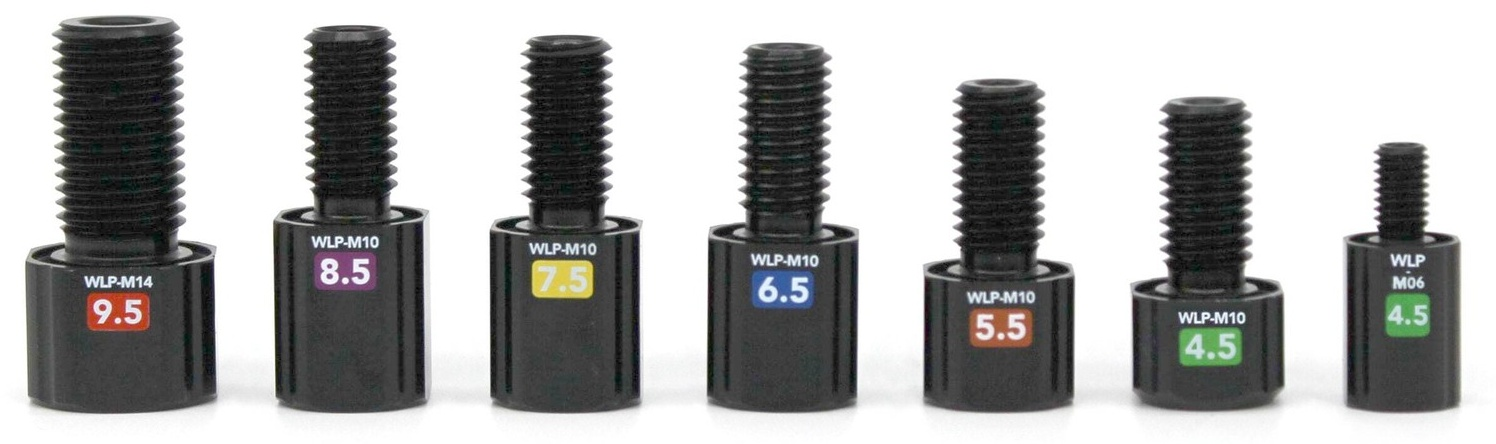
\includegraphics[height=1.75cm, width=\textwidth, keepaspectratio]{wetlink_penetrator_clean.jpg}\\
        \vspace{0.15em}
        \tech{1. WetLink Penetrator Standard (WLP)}\\
        \tiny\textit{Compression sur isolants individuels $\cdot$ Haute pression \textbf{950 m}}
      \end{center}
      \scriptsize
      \begin{itemize}\setlength{\itemsep}{1.5pt}\setlength{\parskip}{0pt}
        \item \textbf{Principe} : compression conique du joint \alertw{sur les conducteurs internes}.
        \item \textbf{Préparation} : nécessite de \alertw{dénuder la gaine extérieure} ($\approx 15\,\text{mm}$).
        \item \textbf{Usage cible} : thrusters T200, ombilic Fathom, traversées haute pression.
      \end{itemize}
    \end{column}

    \begin{column}{0.48\textwidth}
      \begin{center}
        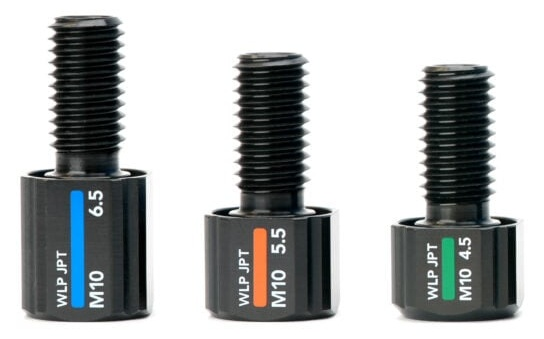
\includegraphics[height=1.75cm, width=\textwidth, keepaspectratio]{wetlink_jpt_clean.jpg}\\
        \vspace{0.15em}
        \succw{2. Nouveau WetLink JPT (Jacket Pass-Through)}\\
        \tiny\textit{Traversée intégrale directe avec gaine $\cdot$ Pression max \textbf{100 m}}
      \end{center}
      \scriptsize
      \begin{itemize}\setlength{\itemsep}{1.5pt}\setlength{\parskip}{0pt}
        \item \textbf{Principe} : \succw{zéro dénudage}, le câble complet traverse avec sa gaine.
        \item \textbf{Étanchéité} : joint conique serrant la gaine ($4.5$, $5.5$ ou $6.5\,\text{mm}$).
        \item \textbf{Usage cible} : coaxiaux d'antenne, blindés vidéo ou capteurs modulaires.
      \end{itemize}
    \end{column}
  \end{columns}
\end{frame}

\begin{frame}{2.5 Pénétrateurs vs Connecteurs : Maintenance \& Modularité}
  \begin{columns}[T]
    \begin{column}{0.49\textwidth}
      \begin{block}{\alertw{Cas Concret : Moteur Défaillant en Manip}}
        \scriptsize
        \begin{itemize}
          \item \textbf{Avec Pénétrateur Fixe (WetLink / Époxy)} :
            \begin{enumerate}\tiny
              \item Rinçage \& séchage intégral extérieur.
              \item Ouvrir le caisson, extraire le tiroir électronique.
              \item Dessouder/dévisser les 3 phases moteur.
              \item Dévisser le contre-écrou interne M10.
              \item Câbler le rechange, refermer, \alertw{refaire 15 min de vide}.
            \end{enumerate}
            $\rightarrow$ \textbf{1h30 d'arrêt}, impossible sur semi-rigide !
          \item \textbf{Avec Connecteur Étanchéifié Externe} :
            \begin{itemize}\tiny
              \item Dévisser la bague, débrancher le moteur en panne.
              \item Brancher le moteur de rechange, revisser la bague.
              \item \succw{2 minutes chrono sans ouvrir le caisson !}
              \item Vide intact, zéro risque d'embruns salés.
            \end{itemize}
        \end{itemize}
      \end{block}
    \end{column}

    \begin{column}{0.49\textwidth}
      \begin{block}{\succw{Modularité "À la Volée" des Capteurs}}
        \scriptsize
        \begin{itemize}
          \item \textbf{Ports Auxiliaires Banalisés} :
            \begin{itemize}\tiny
              \item Embases traversée de coque pré-câblées (série, I2C, CAN, Ethernet, 12V/24V).
              \item Port libre = scellé par un bouchon étanche (*dummy plug*).
            \end{itemize}
          \item \textbf{Flexibilité selon la mission du jour} :
            \begin{itemize}\tiny
              \item \textit{Matin (bathymétrie)} : échosondeur Ping / MBES.
              \item \textit{Après-midi (physico-chimie)} : sonde CTD / fluorimètre.
              \item \textit{Soir (prélèvements)} : pince Newton / phares Lumen.
            \end{itemize}
          \item Véhiculent signaux blindés ET forte puissance ($10\text{--}20\,\text{A}$).
        \end{itemize}
      \end{block}
    \end{column}
  \end{columns}
\end{frame}

\begin{frame}{2.6 Standards de Connectique : Blue Trail Cobalt \& SubConn}
  \begin{columns}[T]
    \begin{column}{0.48\textwidth}
      \begin{center}
        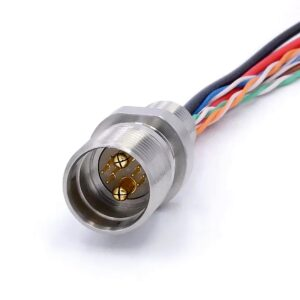
\includegraphics[height=1.7cm, keepaspectratio]{bluetrail_cobalt.jpg}
        \hspace{0.2cm}
        
\includegraphics[height=1.7cm, keepaspectratio]{bluetrail_cobalt_pair.png}
      \end{center}
      \vspace{-0.2em}
      \begin{block}{\tech{Blue Trail Engineering --- Série Cobalt}}
        \scriptsize
        \textbf{\textit{Embase M10 compacte, PEEK / Inox 316, 600\,m (60\,bar)}}\\[0.3em]
        \begin{itemize}\setlength{\itemsep}{1pt}\setlength{\parskip}{0pt}
          \item \textbf{Compatibilité native BlueRobotics} : filetage \textbf{M10} (Cobalt 10), remplace directement un WetLink sans usinage !
          \item Coque inox 316L, inserts PEEK rigides, contacts or.
          \item 3 à 8 pins (M10) et jusqu'à 12 pins / Ethernet (Cobalt 14, M14).
        \end{itemize}
      \end{block}
    \end{column}

    \begin{column}{0.48\textwidth}
      \begin{center}
        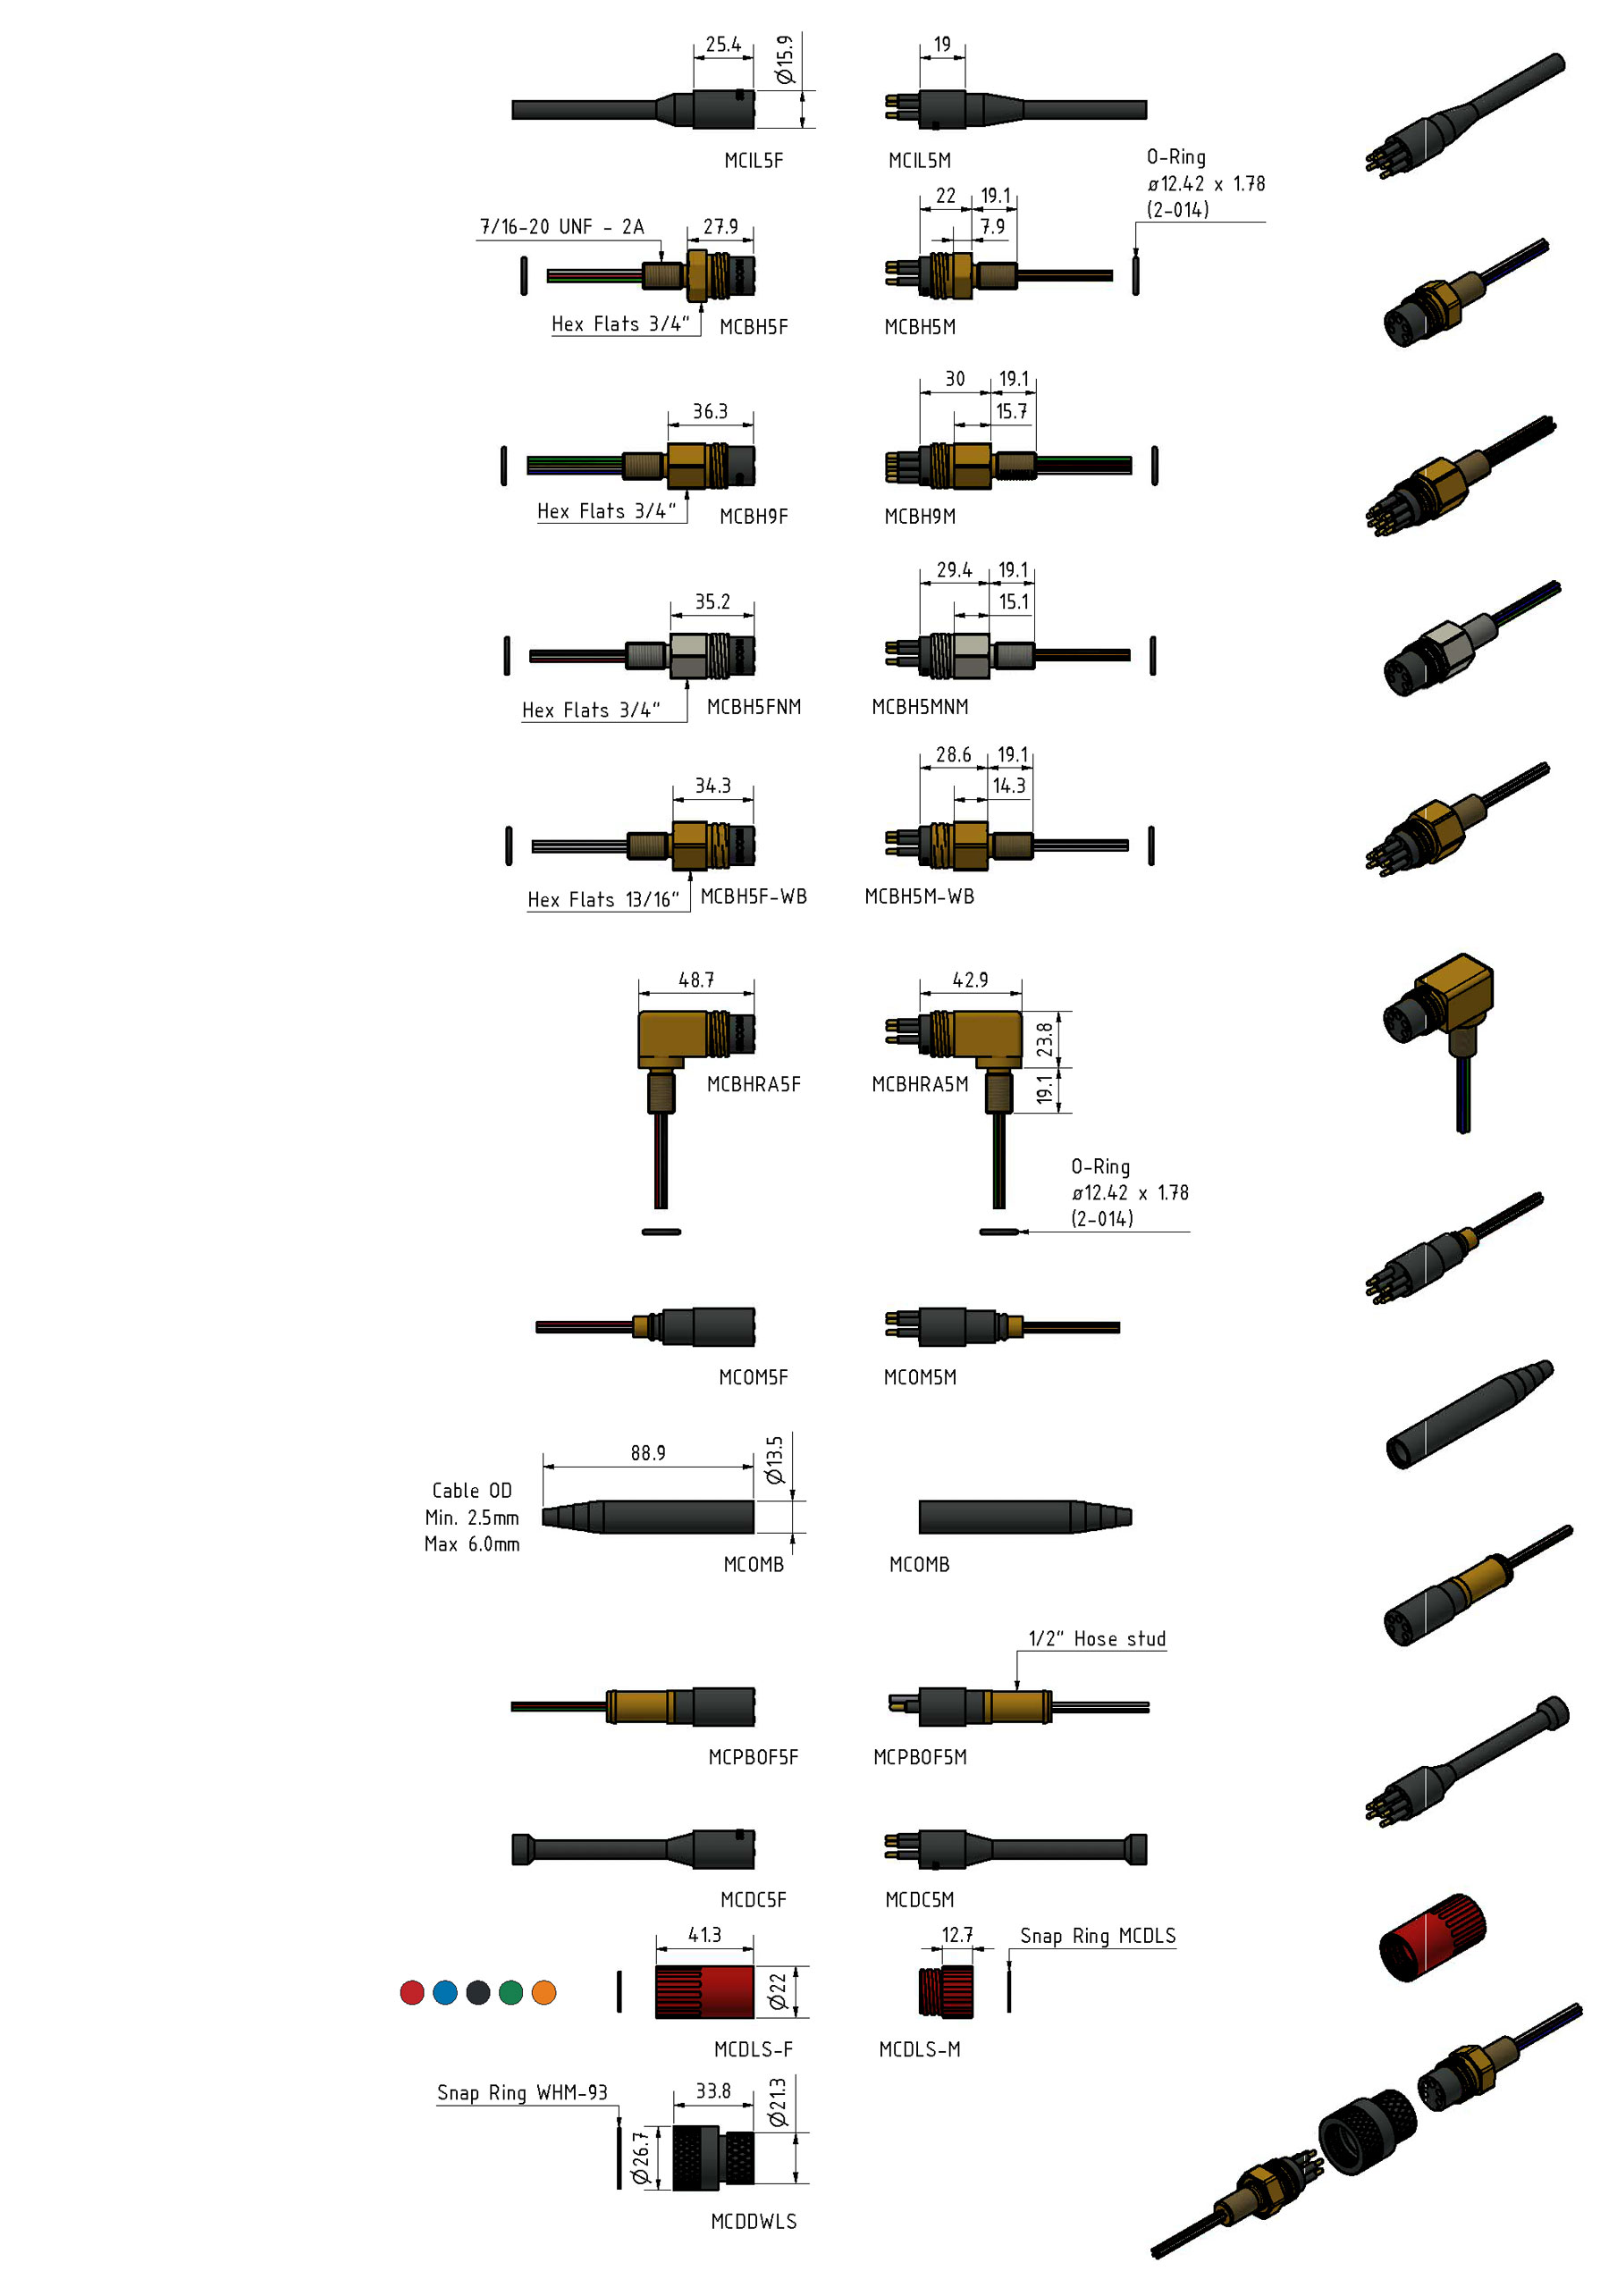
\includegraphics[height=1.7cm, keepaspectratio]{subconn_micro_circular.jpg}
      \end{center}
      \vspace{-0.2em}
      \begin{block}{\tech{SubConn (MacArtney) --- Micro Circular}}
        \scriptsize
        \textbf{\textit{Standard mondial offshore \& océanographie, néoprène}}\\[0.3em]
        \begin{itemize}\setlength{\itemsep}{1pt}\setlength{\parskip}{0pt}
          \item \textbf{Standard historique de l'industrie} : éprouvé depuis plus de 40 ans (Ifremer, navires océanographiques).
          \item Corps surmoulé néoprène souple, bague de verrouillage (*locking sleeve*), haute résistance mécanique.
          \item 2 à 21 contacts, haute tension ($600\,\text{V}$, $10\text{--}15\,\text{A}$).
        \end{itemize}
      \end{block}
    \end{column}
  \end{columns}
\end{frame}

\begin{frame}{2.6b Typologie Opérationnelle : Connectique Dry-Mate vs Wet-Mate}
  \begin{columns}[T]
    \begin{column}{0.49\textwidth}
      \begin{block}{\succw{1. Connecteurs Dry-Mate (Standard Drone)}}
        \scriptsize
        \begin{itemize}
          \item \textbf{Principe} : accouplement et verrouillage effectués \textbf{au sec obligatoirement} sur le pont avant immersion.
          \item Enduction d'un très léger film de graisse silicone sur les fiches.
          \item Étanchéité parfaite jusqu'à 600--2000 m une fois verrouillé.
          \item \succw{Économique, ultra-fiable} et parfaitement adapté aux ROVs/AUVs de laboratoire (Cobalt, SubConn).
        \end{itemize}
      \end{block}
    \end{column}

    \begin{column}{0.49\textwidth}
      \begin{alertblock}{2. Connecteurs Wet-Mate (Haute Technicité)}
        \scriptsize
        \begin{itemize}
          \item \textbf{Principe} : connectable et déconnectable \textbf{directement sous l'eau} en pleine immersion.
          \item Bain d'huile diélectrique interne et membranes racleuses chassant l'eau de mer salée lors de l'enfichage.
          \item \alertw{Extrêmement onéreux} ($>3\,000$ à $8\,000$ € par connecteur).
          \item Réservé aux observatoires fond de mer câblés (EMSO, KM3NeT) et stations d'accueil AUV sous-marines.
        \end{itemize}
      \end{alertblock}
    \end{column}
  \end{columns}
\end{frame}

\begin{frame}{2.7 Gestion de la Pression Caisson : Vents, PRV \& Pompes à Vide}
  \begin{columns}[T]
    \begin{column}{0.32\textwidth}
      \begin{center}
        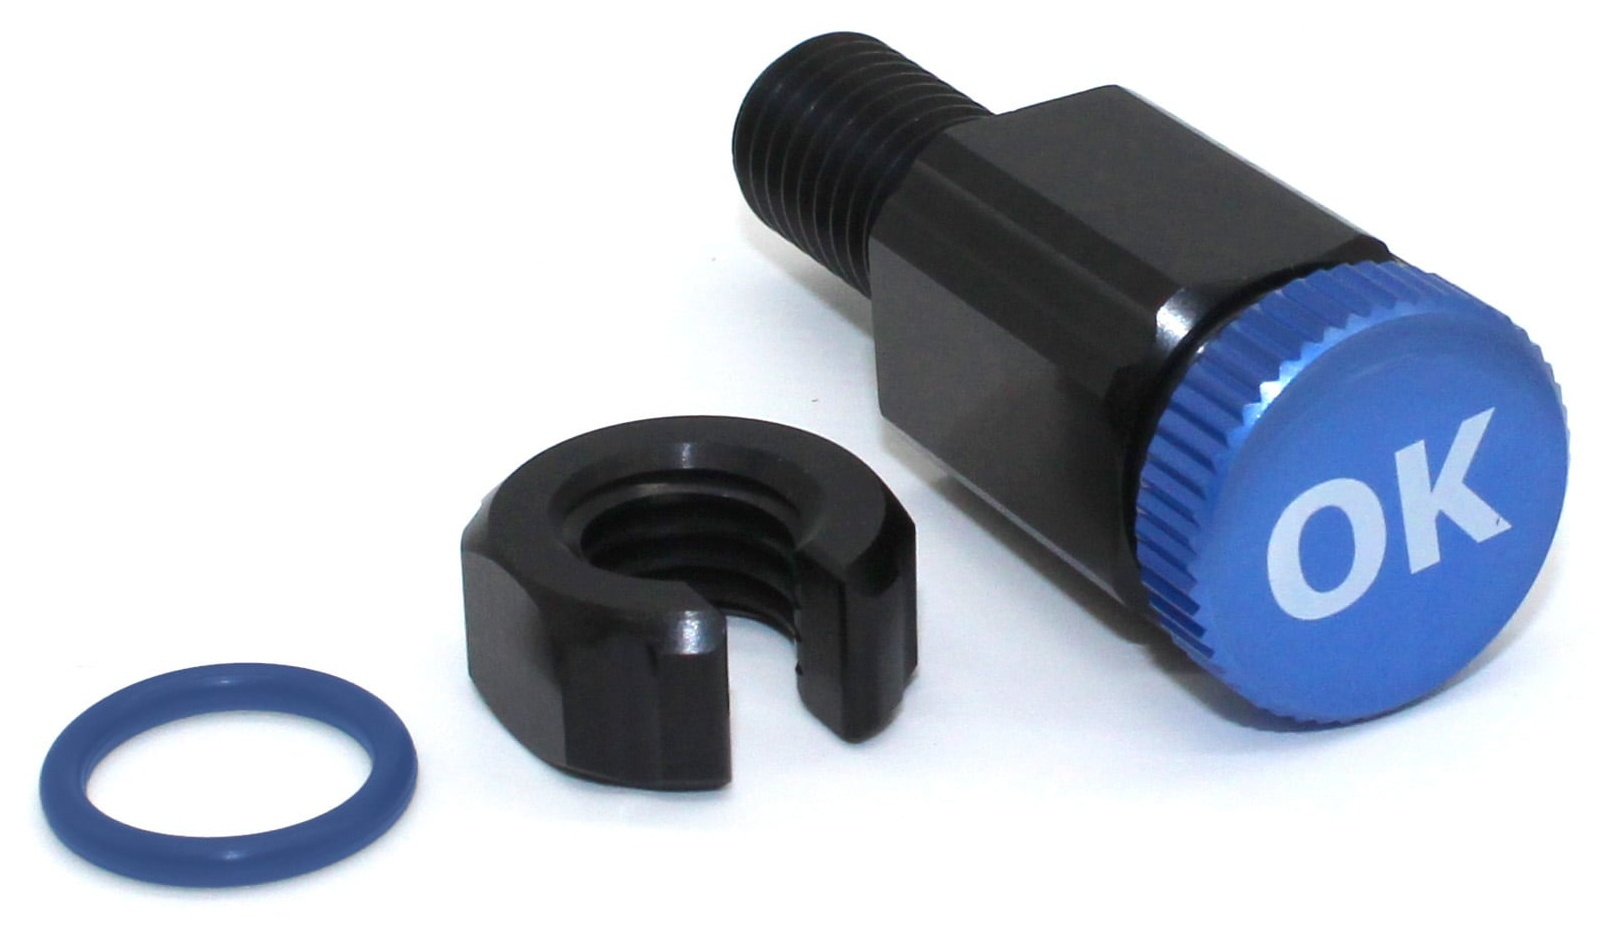
\includegraphics[height=1.35cm, keepaspectratio]{vent_plug_clean.jpg}\\
        \vspace{0.1em}
        \tech{Enclosure Vent and Plug}\\
        \footnotesize\textbf{Bouchon d'Évent M10}
      \end{center}
      \scriptsize
      \begin{itemize}\setlength{\itemsep}{1pt}\setlength{\parskip}{0pt}
        \item \textbf{Équilibrage de pression} : dévissage manuel partiel pour « casser le vide » sans forcer sur les portées ni abîmer les joints.
        \item \textbf{Accès direct sans outil} : bouchon moleté avec double joint torique pour maintenance rapide sur le pont.
        \item \textbf{Port de test dédié} : reçoit l'embout étanche pour le tirage au vide terrain.
      \end{itemize}
    \end{column}

    \begin{column}{0.32\textwidth}
      \begin{center}
        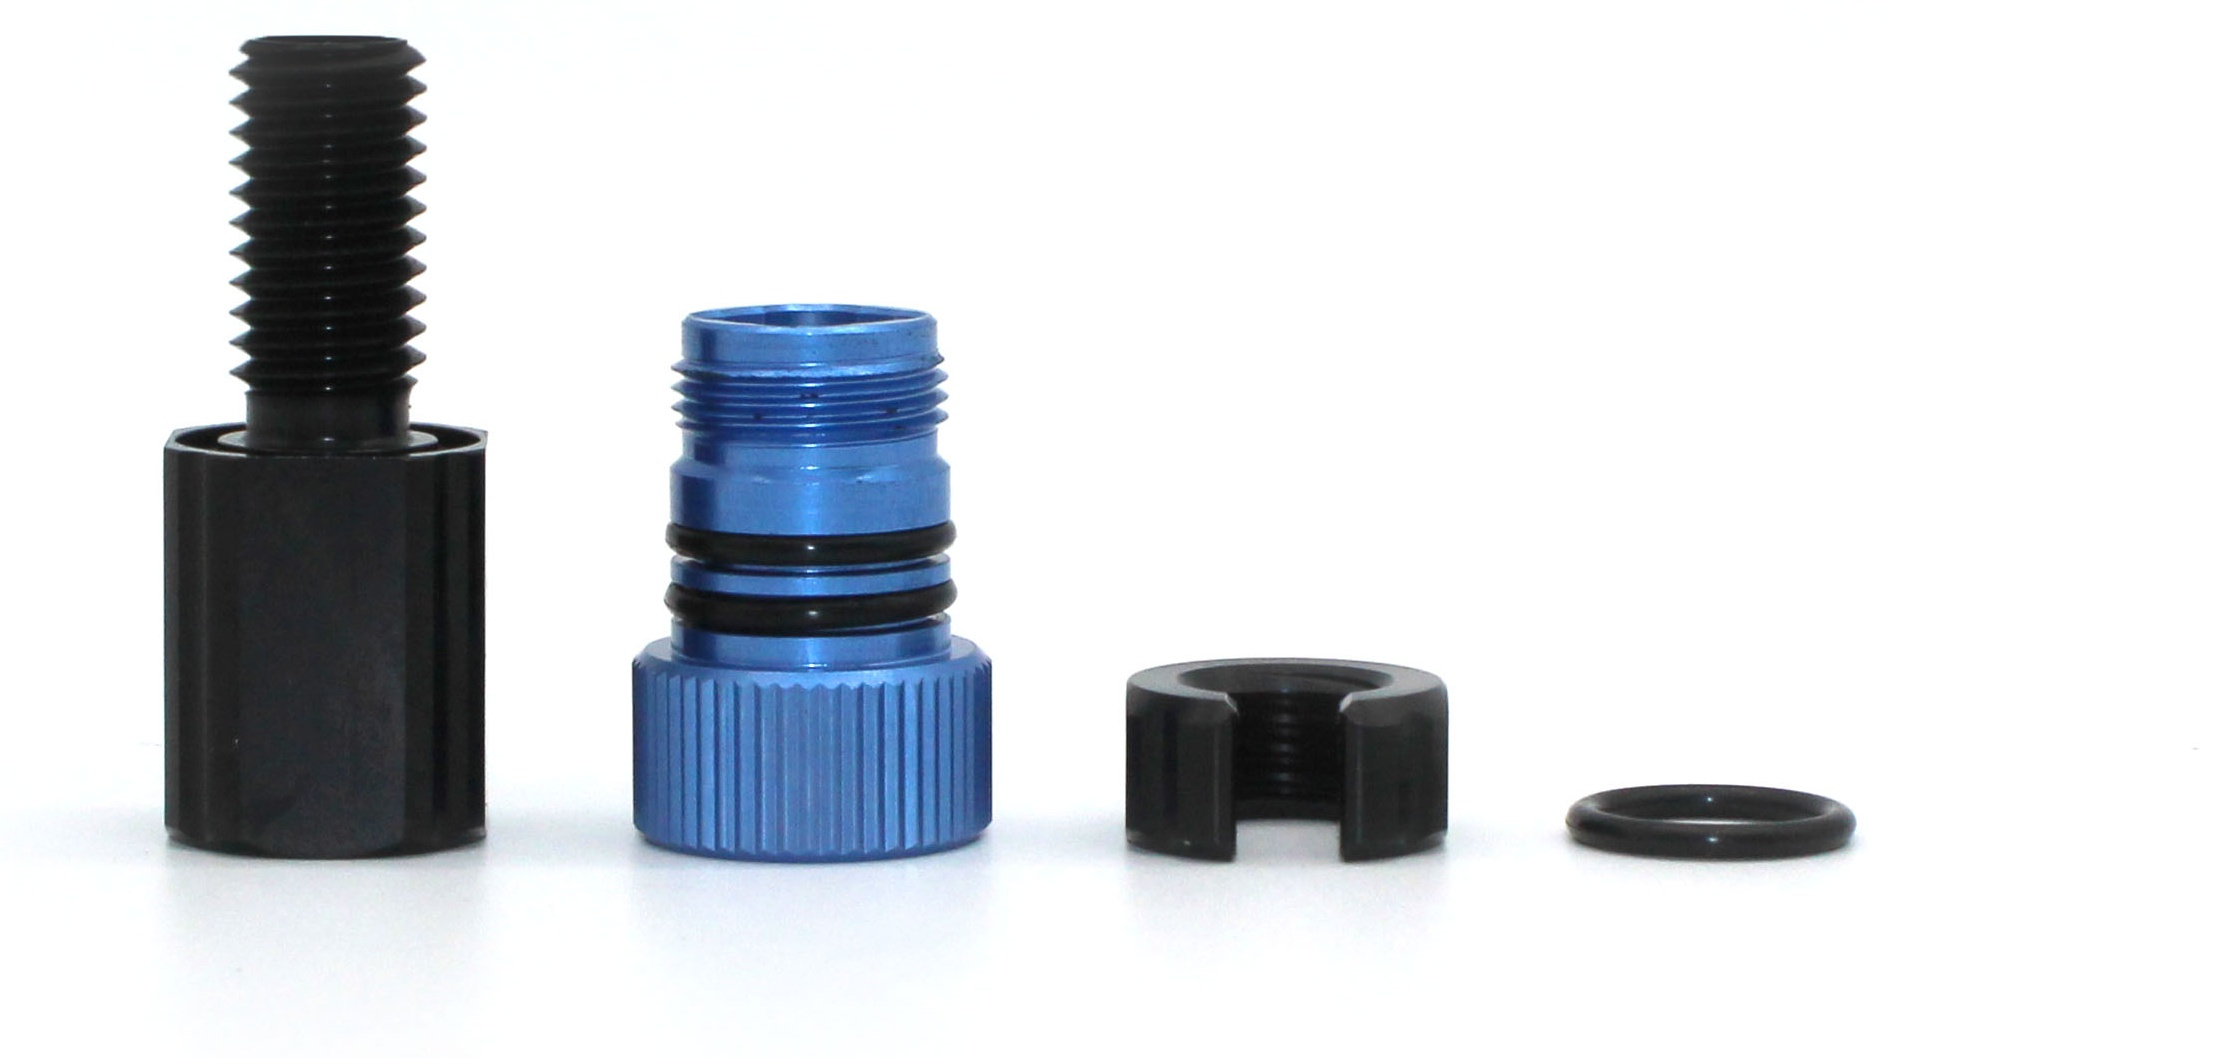
\includegraphics[height=1.35cm, keepaspectratio]{pressure_relief_valve_clean.jpg}\\
        \vspace{0.1em}
        \alertw{Pressure Relief Valve (PRV)}\\
        \footnotesize\textbf{Soupape de Surpression M10}
      \end{center}
      \scriptsize
      \begin{itemize}\setlength{\itemsep}{1pt}\setlength{\parskip}{0pt}
        \item \textbf{Sécurité passive critique} : obligatoire pour tout caisson abritant des batteries \textbf{Li-Ion / LiPo}.
        \item \textbf{Dégazage \& emballement} : évacuation automatique de surpression ($>30\text{--}50\,\text{kPa}$) évitant l'effet « missile » (éjection brutale de flasque).
        \item \textbf{Clapet taré à ressort} : purge les gaz et se referme immédiatement pour préserver l'étanchéité à l'eau.
      \end{itemize}
    \end{column}

    \begin{column}{0.32\textwidth}
      \begin{center}
        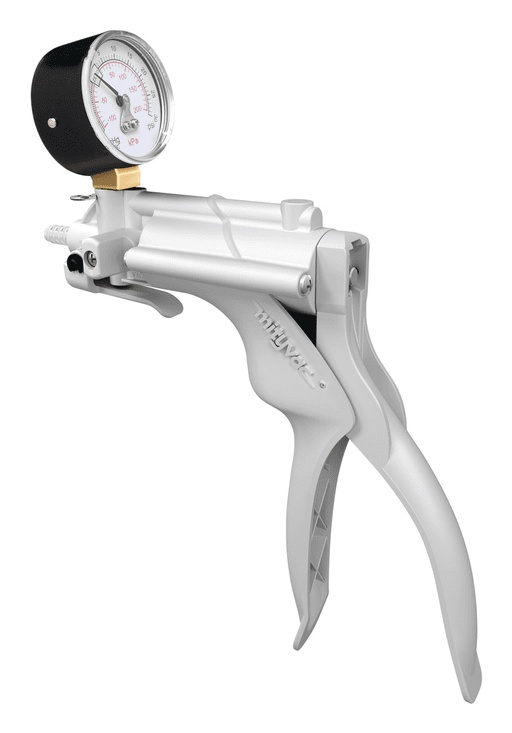
\includegraphics[height=1.5cm, keepaspectratio]{vacuum_pump_clean.jpg}\\
        \vspace{0.1em}
        \succw{Pompe Manuelle à Vide}\\
        \footnotesize\textbf{Testeur de Dépression Terrain}
      \end{center}
      \scriptsize
      \begin{itemize}\setlength{\itemsep}{1pt}\setlength{\parskip}{0pt}
        \item \textbf{Tirage au vide pré-vol} : création d'une dépression relative de \succw{$\mathbf{-0.5\,\text{bar}}$} pour valider l'étanchéité.
        \item \textbf{Manomètre} : détection des micro-fuites sur 15 min.
        \item \textbf{Précharge mécanique} : plaque et verrouille fermement les flasques avant contact avec l'eau.
      \end{itemize}
    \end{column}
  \end{columns}
\end{frame}

\begin{frame}{2.7b Validation Pré-Vol : Le Test de Vide Terrain (Vacuum Test)}
  \begin{alertblock}{La règle d'or absolue avant chaque mise à l'eau}
    Ne jamais immerger un caisson sans avoir validé son étanchéité par dépression.
  \end{alertblock}

  \begin{columns}[T]
    \begin{column}{0.54\textwidth}
      \textbf{Procédure opératoire de terrain} :
      \begin{enumerate}\setlength{\itemsep}{2pt}
        \item Visser l'adaptateur \tech{Vacuum Plug} sur l'évent M10 du caisson.
        \item Raccorder la \tech{pompe à dépression} équipée d'un manomètre de précision.
        \item Pomper pour descendre la pression interne à \succw{$\mathbf{-0.5\,\text{bar}}$ (50 kPa sous le vide relatif)}.
        \item Relever la pression après \textbf{10 minutes} et \textbf{15 minutes} en la lisant sur le manomètre.
        \item Si la pression remonte : \alertw{fuite détectée !} Ne pas plonger.
      \end{enumerate}
    \end{column}

    \begin{column}{0.44\textwidth}
      \begin{center}
        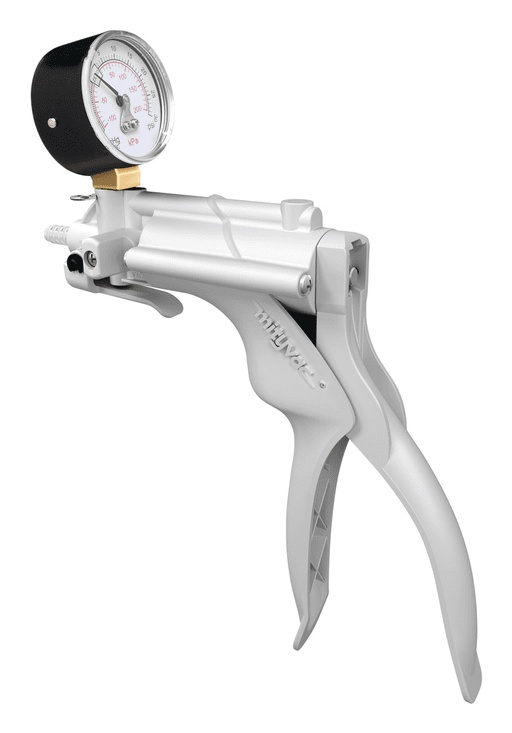
\includegraphics[height=1.9cm, keepaspectratio]{vacuum_pump_clean.jpg}
        \hspace{0.2cm}
        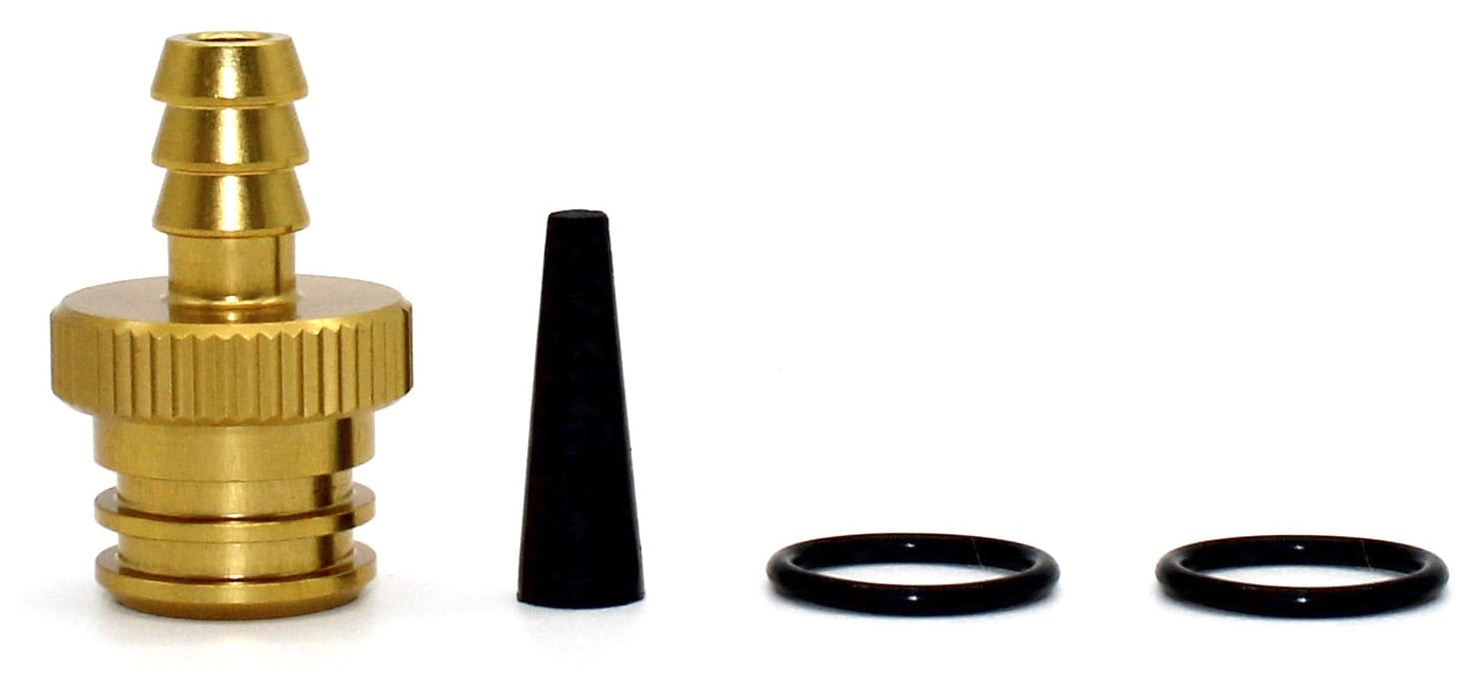
\includegraphics[height=1.3cm, keepaspectratio]{vacuum_plug_clean.jpg}\\
        \vspace{0.1em}
        \tiny\textit{Kit de test à dépression : pompe manuelle \& embout d'évent}
      \end{center}
      \vspace{-0.2em}
      \begin{block}{Causes typiques de fuite}
        \scriptsize
        \begin{itemize}\setlength{\itemsep}{1pt}
          \item Un cheveu ou un grain de sable sur le joint torique.
          \item Excès de graisse silicone ayant piégé une impureté.
          \item Pénétrateur WetLink ou embase connecteur mal serrée sur la flasque.
        \end{itemize}
      \end{block}
    \end{column}
  \end{columns}
\end{frame}

\begin{frame}{2.8 Conception d'un Vecteur de Surface : Le BlueBoat (ASV)}
  \begin{columns}[c]
    \begin{column}{0.42\textwidth}
      \begin{center}
        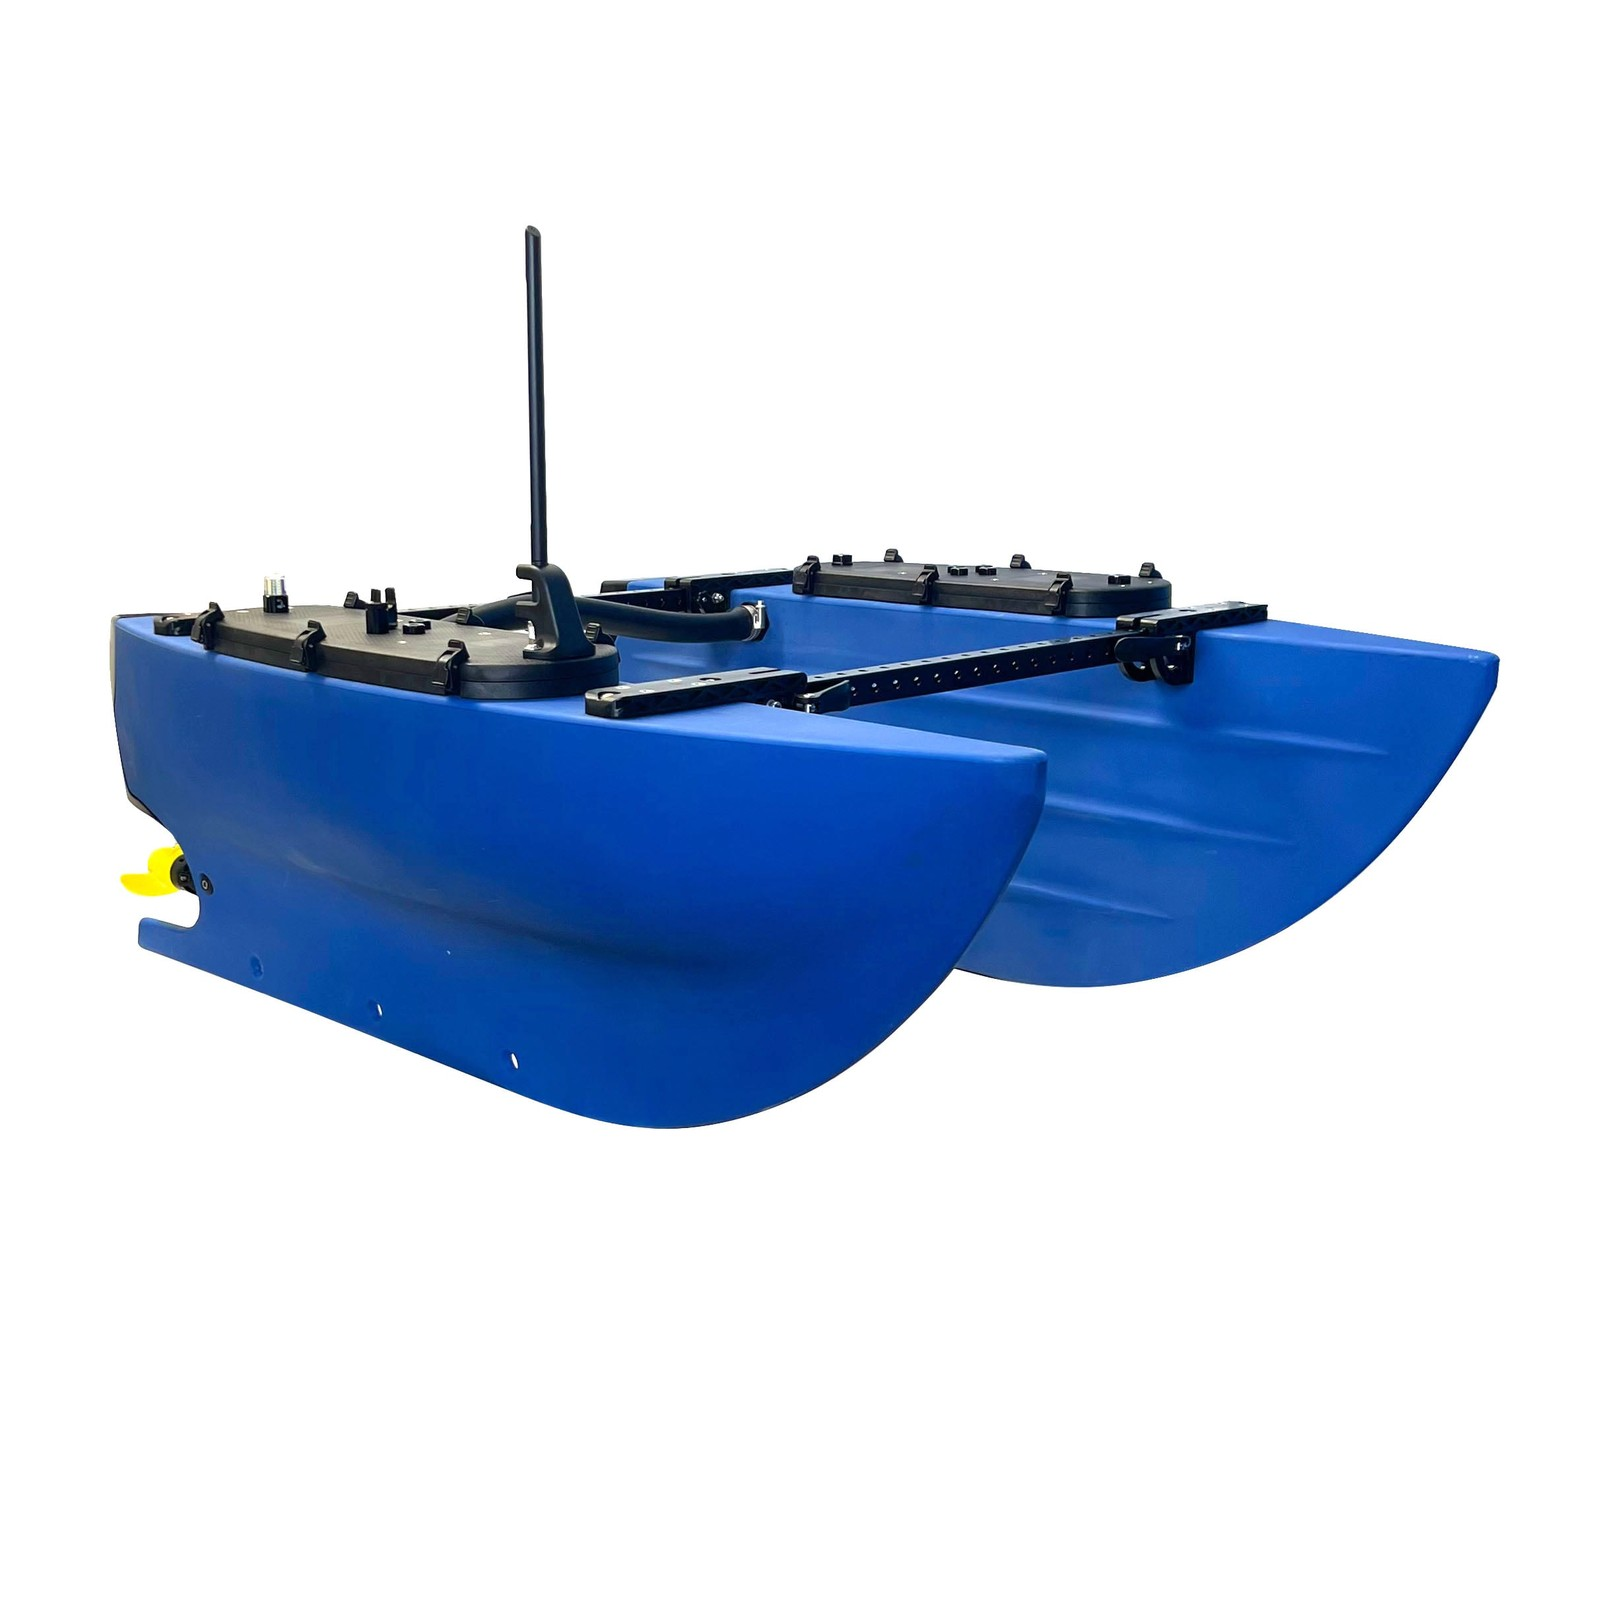
\includegraphics[width=\textwidth, height=4.2cm, keepaspectratio]{blueboat.jpg}\\
        \vspace{0.2em}
        \small\textbf{BlueBoat} (BlueRobotics)\\
        \scriptsize\textit{Catamaran PEHD rotomoulé, 2x T200, baie centrale d'instruments}
      \end{center}
    \end{column}

    \begin{column}{0.56\textwidth}
      \textbf{Architecture \& Caractéristiques} :
      \scriptsize
      \begin{itemize}
        \item \textbf{Coque catamaran} en polyéthylène rotomoulé : quasi-insensible aux impacts contre roches et quais.
        \item Tirant d'eau très faible ($\approx 15\,\text{cm}$) pour lagunes, estuaires et rivières.
        \item \textbf{Propulsion différentielle (*skid-steering*)} : 2 propulseurs T200 avec pâles anti-algues.
        \item \textbf{Baie centrale ouverte} : barres profilées pour fixer ADCP, échosondeurs, sondes CTD.
        \item Pliable sans outil pour transport en voiture.
      \end{itemize}

      \vspace{0.3em}
      \begin{block}{Atouts pour la Recherche}
        \scriptsize
        \begin{itemize}
          \item Autonomie : jusqu'à \textbf{8 à 10 heures} de levé continu ($14.8\,\text{V}$ $30\text{Ah}$).
          \item GNSS : localisation metrique.
          \item Télémétrie WiFi longue portée ($>500\,\text{m}$) ou lien 4G.
        \end{itemize}
      \end{block}
    \end{column}
  \end{columns}
\end{frame}

\begin{frame}{2.8b Architecture Interne du BlueBoat : Électronique \& Propulsion}
  \centering
  \begin{tikzpicture}[
    scale=0.74, every node/.style={transform shape},
    box/.style={rounded corners=3pt, align=center, line width=0.8pt},
    pwr/.style={line width=1.6pt, OceanCoral, -{Latex[length=2.0mm]}},
    pwr5v/.style={line width=1.1pt, OceanCoral!85!black, dashed, -{Latex[length=1.7mm]}},
    sig/.style={line width=1.0pt, OceanCyan!90!black, dashed, -{Latex[length=1.7mm]}},
    net/.style={line width=1.3pt, OceanLight, <->, >=Latex},
    mot/.style={line width=1.6pt, DarkSlate, -{Latex[length=2.0mm]}},
    wlp/.style={draw=OceanDeep, fill=yellow!45, line width=1.1pt, rounded corners=2pt, font=\bfseries, align=center},
    badge/.style={fill=white, rounded corners=2pt, inner sep=1.1pt, font=\tiny\bfseries}
  ]

    % 1. Zone Coques étanches (Hulls)
    \fill[OceanGray!35, rounded corners=6pt] (-0.45, 0.32) rectangle (10.35, 5.05);
    \draw[OceanMedium, line width=1.4pt, rounded corners=6pt] (-0.45, 0.32) rectangle (10.35, 5.05);
    
    % Titre bandeau de la coque étanche
    \node[anchor=south west, fill=OceanMedium, text=white, font=\tiny\bfseries, rounded corners=2pt, inner sep=2.5pt] at (-0.20, 5.05) {%
      ~COQUE ÉTANCHE DU BLUEBOAT (PEHD rotomoulé --- 1\,atm sec)~%
    };

    % 2. Zone Extérieure (Milieu aquatique)
    \fill[OceanCyan!8, rounded corners=6pt] (10.75, 0.32) rectangle (14.55, 5.05);
    \draw[OceanCyan!60, dashed, line width=1.2pt, rounded corners=6pt] (10.75, 0.32) rectangle (14.55, 5.05);
    
    % Titre bandeau milieu extérieur
    \node[anchor=south, fill=OceanCyan!85!black, text=white, font=\tiny\bfseries, rounded corners=2pt, inner sep=2.5pt] at (12.65, 5.05) {%
      ~MILIEU MARIN EXTÉRIEUR (Immergé)~%
    };
    \node[anchor=north, font=\tiny\itshape, text=OceanCyan!85!black] at (12.65, 4.95) {(Eau de mer / Pression hydrostatique)};

    % 3. Calcul, GNSS & Télécoms (x = 0.40 à 2.10)
    \node[box, draw=OceanDeep, fill=white, minimum width=1.45cm, minimum height=0.72cm] (gnss) at (0.40, 3.90) {
      \textbf{\scriptsize GNSS}
    };

    \node[box, draw=OceanLight, fill=OceanLight!15, minimum width=1.45cm, minimum height=0.72cm] (wifi) at (2.10, 3.90) {
      \textbf{\scriptsize Routeur WiFi}\\
      \tiny Liaison sol $2.4/5\,$G
    };

    \node[box, draw=OceanDeep, fill=OceanDeep!15, minimum width=2.5cm, minimum height=0.72cm] (rpi) at (1.25, 2.40) {
      \textbf{\scriptsize Raspberry Pi 4}\\
      \tiny Compagnon (BlueOS)
    };

    \node[box, draw=OceanCyan, fill=OceanCyan!15, minimum width=2.5cm, minimum height=0.72cm] (nav) at (1.25, 0.95) {
      \textbf{\scriptsize Navigator (HAT)}\\
      \tiny Autopilote ArduRover
    };

    % Antennes sur le pont (vers le ciel)
    \draw[line width=1.2pt, OceanDeep] (gnss.north) -- ++(0, 0.38);
    \node[anchor=south, badge, draw=OceanDeep!60, fill=white, text=OceanDeep] at ($(gnss.north)+(0, 0.38)$) {Antenne GNSS};

    \draw[line width=1.2pt, OceanLight] (wifi.north) -- ++(0, 0.38);
    \node[anchor=south, badge, draw=OceanLight!60, fill=OceanLight!10, text=OceanLight] at ($(wifi.north)+(0, 0.38)$) {Antenne WiFi};

    % Liaisons internes Calcul (Gauche) : strictement verticales
    \draw[sig, OceanDeep, line width=1.1pt] (gnss.south) -- ($(rpi.north)-(0.85, 0)$) 
      node[midway, badge, draw=OceanDeep!40, text=OceanDeep]{USB/NMEA};
    \draw[net] (wifi.south) -- ($(rpi.north)+(0.85, 0)$) 
      node[midway, badge, draw=OceanLight!40, text=OceanLight]{Ethernet};
    \draw[net, OceanCyan, line width=1.4pt] (rpi) -- (nav) 
      node[midway, badge, draw=OceanCyan!40, text=OceanCyan!90!black]{Bus HAT (GPIO)};

    % 4. Énergie (Colonne 2, x = 4.75)
    \node[box, draw=OceanCoral, fill=OceanCoral!15, minimum width=2.5cm, minimum height=0.75cm] (bat) at (4.75, 3.90) {
      \textbf{\scriptsize Batteries Li-Ion}\\
      \tiny $14.8\,\text{V}$ (4S, $18\text{--}30\,\text{Ah}$)
    };

    \node[box, draw=OceanCoral!85!black, fill=white, minimum width=2.6cm, minimum height=0.90cm] (pdb) at (4.75, 2.40) {
      \textbf{\scriptsize Carte Distribution (PDB)}\\
      \tiny Shunt $U/I$ \& Régulateurs BEC
    };

    % Liaison Batterie vers PDB
    \draw[pwr, line width=2.0pt] (bat) -- (pdb) node[midway, badge, draw=OceanCoral!40, text=OceanCoral!90!black]{14.8\,V (VBAT)};

    % Alimentations régulées depuis PDB
    % 5V BEC vers RPi : horizontal direct à y = 2.22
    \draw[pwr5v] ($(pdb.west)-(0, 0.18)$) -- ($(rpi.east)-(0, 0.18)$) 
      node[midway, badge, draw=OceanCoral!40, text=OceanCoral!85!black]{5\,V BEC};
    
    % 12V vers WiFi : sort à y = 2.62, monte par x = 3.15 dégagé
    \draw[pwr5v] ($(pdb.west)+(0, 0.22)$) -- (3.15, 2.62) -- (3.15, 3.90) -- (wifi.east);
    \node[badge, draw=OceanCoral!40, text=OceanCoral!85!black] at (3.15, 3.25) {12\,V};

    % 5. Variateurs ESC (Colonne 3, x = 7.95)
    \node[box, draw=OceanGreen, fill=OceanGreen!15, minimum width=2.0cm, minimum height=0.75cm] (esc_b) at (7.95, 3.90) {
      \textbf{\scriptsize ESC Bâbord}\\
      \tiny Basic ESC (30\,A)
    };

    \node[box, draw=OceanGreen, fill=OceanGreen!15, minimum width=2.0cm, minimum height=0.75cm] (esc_t) at (7.95, 0.95) {
      \textbf{\scriptsize ESC Tribord}\\
      \tiny Basic ESC (30\,A)
    };

    % Alimentation puissance 14.8V PDB vers ESCs (Couloir x in [6.05, 6.95])
    % Vers ESC Bâbord (monte par x = 6.45, entre par le haut à y = 4.05)
    \draw[pwr] ($(pdb.east)+(0, 0.20)$) -- (6.45, 2.60) -- (6.45, 4.05) -- ($(esc_b.west)+(0, 0.15)$);
    \node[badge, draw=OceanCoral!40, text=OceanCoral!90!black] at (6.45, 3.35) {14.8\,V};

    % Vers ESC Tribord (descend par x = 6.45, entre par le haut à y = 1.10)
    \draw[pwr] ($(pdb.east)-(0, 0.20)$) -- (6.45, 2.20) -- (6.45, 1.10) -- ($(esc_t.west)+(0, 0.15)$);
    \node[badge, draw=OceanCoral!40, text=OceanCoral!90!black] at (6.45, 1.65) {14.8\,V};

    % Commandes PWM Moteurs (Nav vers ESCs) : aucun croisement, cheminements strictement horizontaux puis verticaux
    % PWM Tribord : direct horizontalement sous la PDB à y = 0.80
    \draw[sig] ($(nav.east)-(0, 0.15)$) -- ($(esc_t.west)-(0, 0.15)$)
      node[pos=0.68, badge, draw=OceanCyan!50, text=OceanCyan!90!black]{PWM Tribord (Servo 2)};

    % PWM Bâbord : horizontal direct à y = 1.20 puis monte par x = 6.75 (entre sous la ligne 14.8V à y = 3.75)
    \draw[sig] ($(nav.east)+(0, 0.25)$) -- (6.75, 1.20) 
      node[pos=0.45, badge, draw=OceanCyan!50, text=OceanCyan!90!black]{PWM Bâbord (Servo 1)}
      -- (6.75, 3.75) -- ($(esc_b.west)-(0, 0.15)$);

    % 6. Pénétrateurs WLP (Frontière de paroi, x = 10.35)
    \node[wlp, minimum width=1.15cm, minimum height=0.62cm] (wlp_b) at (10.35, 3.90) {
      \textbf{\tiny WLP}\\
      \tiny M10
    };

    \node[wlp, minimum width=1.15cm, minimum height=0.62cm] (wlp_t) at (10.35, 0.95) {
      \textbf{\tiny WLP}\\
      \tiny M10
    };

    % Encadré d'explication des Pénétrateurs WLP (centré sur la paroi)
    \node[badge, draw=OceanDeep, fill=yellow!25, line width=0.8pt, align=center, text=OceanDeep] (wlp_info) at (10.35, 2.40) {%
      \textbf{\tiny Traversée Étanche}\\[-0.2ex]
      \tiny Pénétrateurs WetLink\\[-0.2ex]
      \tiny (\textit{Écrou M10 étanche})%
    };
    \draw[line width=0.7pt, OceanDeep, ->] (wlp_info.north) -- (wlp_b.south);
    \draw[line width=0.7pt, OceanDeep, ->] (wlp_info.south) -- (wlp_t.north);

    % 7. Propulseurs T200 (Extérieur, x = 12.65)
    \node[box, draw=OceanDeep, fill=OceanDeep!18, minimum width=2.4cm, minimum height=0.85cm] (t200_b) at (12.65, 3.90) {
      \textbf{\scriptsize Propulseur T200}\\
      \tiny Moteur Bâbord (\textit{Port})
    };

    \node[box, draw=OceanDeep, fill=OceanDeep!18, minimum width=2.4cm, minimum height=0.85cm] (t200_t) at (12.65, 0.95) {
      \textbf{\scriptsize Propulseur T200}\\
      \tiny Moteur Tribord (\textit{Starboard})
    };

    % Traversée de paroi étanche WLP vers T200 (Câbles moteurs triphasés)
    \draw[mot] (esc_b.east) -- (wlp_b.west) node[midway, badge, draw=DarkSlate!30, text=DarkSlate]{3 phases};
    \draw[mot] (wlp_b.east) -- (t200_b.west);

    \draw[mot] (esc_t.east) -- (wlp_t.west) node[midway, badge, draw=DarkSlate!30, text=DarkSlate]{3 phases};
    \draw[mot] (wlp_t.east) -- (t200_t.west);

    % Légende synthétique en bas
    \node[anchor=west, font=\tiny, text=DarkSlate] at (-0.35, 0.08) {%
      \textbf{Flux :}~
      \textcolor{OceanCoral}{\rule[0.5ex]{8pt}{1.8pt}}~\textbf{14.8\,V (VBAT)}\quad
      \textcolor{OceanCoral!85!black}{\textbf{- -}~\textbf{BEC 5V/12V}}\quad
      \textcolor{OceanCyan!90!black}{\textbf{- -}~\textbf{PWM}}\quad
      \textcolor{OceanDeep}{\textbf{- -}~\textbf{USB/NMEA}}\quad
      \textcolor{OceanLight}{\textbf{$\leftrightarrow$}~\textbf{Ethernet/HAT}}\quad
      \textcolor{DarkSlate}{\rule[0.5ex]{8pt}{1.6pt}}~\textbf{Triphasé}%
    };

  \end{tikzpicture}

  \vspace{0.1em}
  \begin{columns}[T, onlytextwidth]
    \begin{column}{0.32\textwidth}
      \begin{block}{\tech{1. Calcul, GNSS \& Sol}}
        \scriptsize
        \textbf{RPi 4} (BlueOS) + \textbf{Navigator} (ArduRover). Le \textbf{GNSS/RTK} assure le cap et positionnement métrique ; le \textbf{routeur WiFi} la liaison sol ($>500\,\text{m}$).
      \end{block}
    \end{column}

    \begin{column}{0.32\textwidth}
      \begin{block}{\succw{2. Puissance \& Distribution}}
        \scriptsize
        \textbf{Batteries Li-Ion} reliées à la \textbf{PDB} : bus forte intensité ($14.8\,\text{V}$) vers ESCs et conversion régulée ($5\,\text{V}$) pour l'électronique.
      \end{block}
    \end{column}

    \begin{column}{0.32\textwidth}
      \begin{block}{\alertw{3. Traversée \& Propulsion}}
        \scriptsize
        Les \textbf{pénétrateurs WetLink (WLP)} assurent l'étanchéité des phases moteurs traversant la coque (\textit{hulls}) vers les \textbf{T200} immergés.
      \end{block}
    \end{column}
  \end{columns}
\end{frame}
\begin{frame}{2.8c Conception d'un Vecteur Sous-Marin : Le BlueROV2 (ROV)}
  \begin{columns}[c]
    \begin{column}{0.42\textwidth}
      \begin{center}
        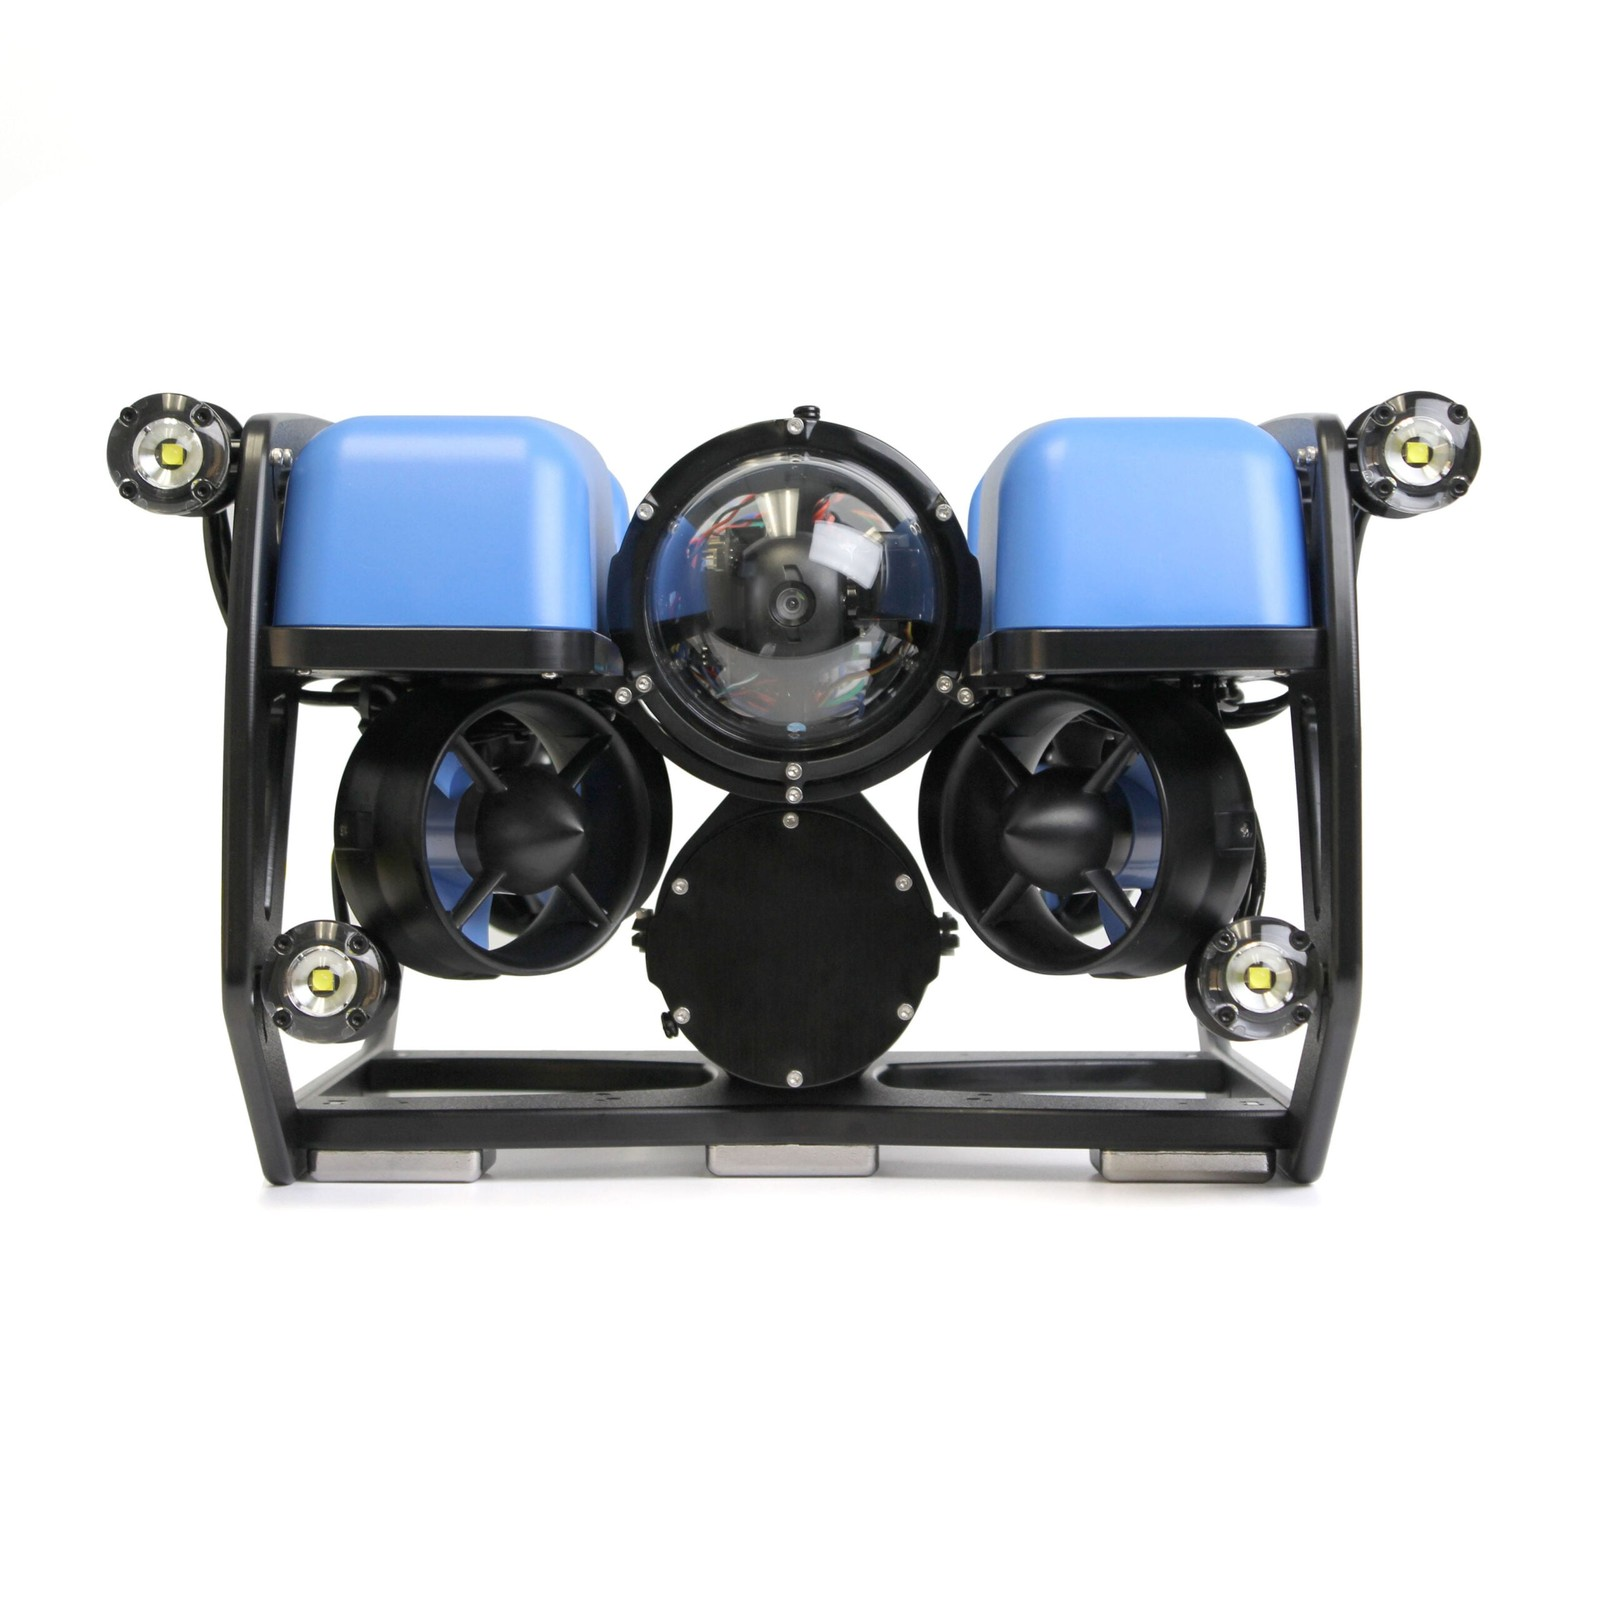
\includegraphics[width=\textwidth, height=4.2cm, keepaspectratio]{bluerov2.jpg}\\
        \vspace{0.2em}
        \small\textbf{BlueROV2} (BlueRobotics)\\
        \scriptsize\textit{Châssis modulaire PEHD, double caisson étanche (4" \& 3"), 6 à 8x T200, ombilical Fathom}
      \end{center}
    \end{column}

    \begin{column}{0.56\textwidth}
      \textbf{Architecture \& Parties Constituantes} :
      \scriptsize
      \begin{itemize}\setlength{\itemsep}{1.5pt}\setlength{\parskip}{0pt}
        \item \textbf{Châssis modulaire en PEHD} : berceau insensible à la corrosion, supportant les blocs de mousse de flottabilité haute ($\overline{BG} > 0$).
        \item \textbf{Double enceinte étanche} : caisson supérieur (tube 4") pour l'électronique \& caisson inférieur (tube 3") pour la batterie.
        \item \textbf{Propulsion vectorisée} : 6 à 8 propulseurs \textbf{T200} (moteurs brushless à rotor noyé) offrant jusqu'à \succw{6 degrés de liberté}.
        \item \textbf{Liaison ombilicale filaire (Tether)} : câble fin à flottabilité neutre transportant le flux réseau haut débit (Fathom-X).
        \item \textbf{Franchissements de flasques} : pénétrateurs \textbf{WetLink (WLP M10)} assurant l'étanchéité jusqu'à $100\text{--}300\,\text{m}$.
      \end{itemize}

      \vspace{0.25em}
      \begin{block}{Atouts pour la Recherche \& l'Observation}
        \scriptsize
        \begin{itemize}\setlength{\itemsep}{1pt}\setlength{\parskip}{0pt}
          \item \textbf{Téléopération temps réel} : flux vidéo HD/4K à faible latence et télémétrie complète sous MAVLink (QGroundControl).
          \item \textbf{Stationnarité parfaite} : tenue de cap et maintien de profondeur automatiques (\textit{Depth Hold} via capteur Bar30).
          \item \textbf{Payload modulaire} : intégration simple de capteurs scientifiques (sonde CTD, sonar Ping360, DVL-A50, balise USBL).
        \end{itemize}
      \end{block}
    \end{column}
  \end{columns}
\end{frame}

\begin{frame}{2.8d Architecture Globale du BlueROV2 : Électronique, Ombilical \& Propulsion}
  \centering
  \begin{tikzpicture}[
    scale=0.72, every node/.style={transform shape},
    box/.style={rounded corners=3pt, align=center, line width=0.8pt},
    pwr/.style={line width=1.6pt, OceanCoral, -{Latex[length=2.0mm]}},
    pwr5v/.style={line width=1.1pt, OceanCoral!85!black, dashed, -{Latex[length=1.7mm]}},
    sig/.style={line width=1.0pt, OceanCyan!90!black, dashed, -{Latex[length=1.7mm]}},
    net/.style={line width=1.3pt, OceanLight, <->, >=Latex},
    mot/.style={line width=1.6pt, DarkSlate, -{Latex[length=2.0mm]}},
    wlp/.style={draw=OceanDeep, fill=yellow!45, line width=1.1pt, rounded corners=2pt, font=\bfseries, align=center},
    badge/.style={fill=white, rounded corners=2pt, inner sep=1.1pt, font=\tiny\bfseries}
  ]

    % 1. Zone Surface / Sol (Topside)
    \fill[OceanGray!35, rounded corners=6pt] (-0.40, 0.70) rectangle (2.30, 5.05);
    \draw[DarkSlate!35, dashed, line width=1.1pt, rounded corners=6pt] (-0.40, 0.70) rectangle (2.30, 5.05);
    \node[anchor=south, fill=DarkSlate, text=white, font=\tiny\bfseries, rounded corners=2pt, inner sep=2.5pt] at (0.95, 5.05) {%
      ~SURFACE (POSTE SOL)~%
    };
    \node[anchor=north, font=\tiny\itshape, text=DarkSlate] at (0.95, 4.95) {(Air / Topside)};

    % 2. Zone Caisson Électronique (Tube 4")
    \fill[OceanGray!35, rounded corners=6pt] (3.90, 0.70) rectangle (11.20, 5.05);
    \draw[OceanMedium, line width=1.4pt, rounded corners=6pt] (3.90, 0.70) rectangle (11.20, 5.05);
    \node[anchor=south west, fill=OceanMedium, text=white, font=\tiny\bfseries, rounded corners=2pt, inner sep=2.5pt] at (4.10, 5.05) {%
      ~CAISSON ÉLECTRONIQUE (Tube 4'' --- Intérieur sec 1\,atm)~%
    };

    % 3. Zone Caisson Batterie (Tube 3")
    \fill[OceanGray!35, rounded corners=6pt] (5.90, -0.80) rectangle (9.50, 0.35);
    \draw[OceanMedium, line width=1.3pt, rounded corners=6pt] (5.90, -0.80) rectangle (9.50, 0.35);
    \node[anchor=north west, font=\tiny\bfseries, text=OceanDeep] at (6.05, 0.30) {Caisson Batterie (Tube 3'' --- $G$ bas)};

    % 4. Zone Milieu Marin Extérieur (Immergé)
    \fill[OceanCyan!8, rounded corners=6pt] (11.60, 0.70) rectangle (15.00, 5.05);
    \draw[OceanCyan!60, dashed, line width=1.2pt, rounded corners=6pt] (11.60, 0.70) rectangle (15.00, 5.05);
    \node[anchor=south, fill=OceanCyan!85!black, text=white, font=\tiny\bfseries, rounded corners=2pt, inner sep=2.5pt] at (13.30, 5.05) {%
      ~MILIEU MARIN EXTÉRIEUR~%
    };
    \node[anchor=north, font=\tiny\itshape, text=OceanCyan!85!black] at (13.30, 4.95) {(Eau de mer / Immersion)};

    % --- Composants Surface / Poste Sol ---
    \node[box, draw=OceanLight, fill=OceanLight!15, minimum width=2.2cm, minimum height=0.75cm] (fxti) at (0.95, 3.90) {
      \textbf{\scriptsize Fathom-X Sol}\\
      \tiny Boîtier FXTI (CPL)
    };

    \node[box, draw=OceanDeep, fill=OceanDeep!10, minimum width=2.2cm, minimum height=0.75cm] (pc) at (0.95, 2.30) {
      \textbf{\scriptsize PC Sol (QGC)}\\
      \tiny Station de pilotage \& Vidéo
    };

    \draw[net] (pc) -- (fxti) node[midway, badge, draw=OceanLight!40, text=OceanLight]{Ethernet};

    \node[anchor=center, font=\tiny, text=DarkSlate!75, align=center] at (0.95, 1.25) {%
      \textbf{QGroundControl (QGC)}\\%
      \textit{Joystick \& MAVLink}%
    };

    % --- Ombilical & Traversée WLP Tether ---
    \node[wlp, minimum width=0.90cm, minimum height=0.55cm] (wlp_tet) at (3.90, 3.90) {\textbf{\tiny WLP}};

    \draw[line width=1.8pt, OceanMedium] (fxti.east) -- (wlp_tet.west)
      node[midway, badge, draw=OceanMedium!40, fill=OceanCyan!10, text=OceanMedium]{Tether (Ombilical)};

    % --- Composants Caisson Électronique ---
    % Colonne 1 : Fathom-X (haut) & RPi 4 (bas)
    \node[box, draw=OceanLight, fill=OceanLight!15, minimum width=1.9cm, minimum height=0.72cm] (fathom_rov) at (5.10, 3.90) {
      \textbf{\scriptsize Fathom-X}\\
      \tiny Modem HomePlug CPL
    };

    \node[box, draw=OceanDeep, fill=OceanDeep!15, minimum width=2.1cm, minimum height=0.75cm] (rpi) at (5.10, 2.35) {
      \textbf{\scriptsize Raspberry Pi 4}\\
      \tiny Compagnon (BlueOS)
    };

    \draw[mot, line width=1.2pt] (wlp_tet.east) -- (fathom_rov.west);
    \draw[net] (fathom_rov) -- (rpi) node[midway, badge, draw=OceanLight!40, text=OceanLight]{RJ45};

    % Colonne 2 : Caméra HD (haut), Navigator HAT (milieu), PDB (bas)
    \node[box, draw=DarkSlate, fill=white, minimum width=2.0cm, minimum height=0.72cm] (cam) at (7.70, 3.90) {
      \textbf{\scriptsize Caméra HD}\\
      \tiny Tilt orientable (Servo)
    };

    \node[box, draw=OceanCyan, fill=OceanCyan!15, minimum width=2.1cm, minimum height=0.75cm] (nav) at (7.70, 2.35) {
      \textbf{\scriptsize Navigator (HAT)}\\
      \tiny Autopilote ArduSub
    };

    \node[box, draw=OceanCoral!85!black, fill=white, minimum width=2.1cm, minimum height=0.68cm] (pdb) at (7.70, 1.15) {
      \textbf{\scriptsize Carte PDB / BEC}\\
      \tiny Shunt $U/I$ \& 5\,V
    };

    % Liaisons RPi <-> Navigator & Caméra
    \draw[net, OceanCyan, line width=1.4pt] (rpi) -- (nav) node[midway, badge, draw=OceanCyan!40, text=OceanCyan!90!black]{Bus HAT (GPIO)};
    \draw[sig] (nav.north) -- (cam.south) node[midway, badge, draw=OceanCyan!40, text=OceanCyan!90!black]{PWM Tilt};
    \draw[sig, OceanDeep] ($(cam.west)-(0, 0.12)$) -| ($(rpi.north)+(0.45, 0)$) 
      node[pos=0.25, badge, draw=OceanDeep!40, text=OceanDeep]{USB Vidéo};

    % Alimentation 5V BEC depuis PDB vers Navigator (qui alimente la RPi par le HAT)
    \draw[pwr5v] ($(pdb.north)-(0.25, 0)$) -- ($(nav.south)-(0.25, 0)$) 
      node[midway, badge, draw=OceanCoral!40, text=OceanCoral!85!black]{5\,V BEC};

    % Colonne 3 : ESCs
    \node[box, draw=OceanGreen, fill=OceanGreen!15, minimum width=1.9cm, minimum height=0.75cm] (esc) at (10.05, 2.35) {
      \textbf{\scriptsize 6--8x ESCs}\\
      \tiny Basic ESCs (30\,A)
    };

    % Commandes PWM Moteurs (Nav -> ESCs)
    \draw[sig] (nav.east) -- (esc.west) node[midway, badge, draw=OceanCyan!40, text=OceanCyan!90!black]{PWM Moteurs};

    % Alimentation puissance 14.8V PDB -> ESCs
    \draw[pwr] ($(pdb.east)+(0, 0.10)$) -- (9.80, 1.25) -- ($(esc.south)-(0.25, 0)$);
    \node[badge, draw=OceanCoral!40, text=OceanCoral!90!black] at (9.25, 1.25) {14.8\,V};

    % --- Pénétrateurs Flasque Arrière (x = 11.20) ---
    \node[wlp, minimum width=0.85cm, minimum height=0.48cm] (wlp_lum) at (11.20, 3.90) {\textbf{\tiny WLP}};
    \node[wlp, minimum width=0.85cm, minimum height=0.48cm] (wlp_mot) at (11.20, 2.35) {\textbf{\tiny WLP}};
    \node[wlp, minimum width=0.85cm, minimum height=0.48cm] (wlp_bar) at (11.20, 1.15) {\textbf{\tiny WLP}};

    \node[font=\tiny\bfseries, text=OceanDeep, align=center] at (11.20, 4.65) {Pénétrateurs\\WetLink (M10)};
    \draw[->, line width=0.7pt, OceanDeep] (11.20, 4.38) -- (wlp_lum.north);

    % Commande PWM Lumen (passe dans le couloir supérieur à y = 3.90)
    \draw[sig] ($(nav.east)+(0, 0.22)$) -- (8.90, 2.57) -- (8.90, 3.90) -- (wlp_lum.west);
    \node[badge, draw=OceanCyan!40, text=OceanCyan!90!black] at (9.85, 3.90) {PWM Lumen};

    % Bus I2C Capteur Bar30 (passe dans le couloir inférieur)
    \draw[sig] ($(nav.east)-(0, 0.22)$) -- (8.90, 2.13) -- (8.90, 0.85) -- (10.65, 0.85) -- (10.65, 1.15) -- (wlp_bar.west);
    \node[badge, draw=OceanCyan!40, text=OceanCyan!90!black] at (9.80, 0.85) {Bus I2C};

    % --- Caisson Batterie & Traversée Puissance ---
    \node[box, draw=OceanCoral, fill=OceanCoral!15, minimum width=3.2cm, minimum height=0.65cm] (bat) at (7.70, -0.25) {
      \textbf{\scriptsize Batterie Li-Ion 4S ($14.8\,\text{V}$)}\\
      \tiny 18\,Ah (266\,Wh) + Switch M10
    };

    \node[wlp, minimum width=0.80cm, minimum height=0.32cm] (wlp_bat) at (7.70, 0.35) {\textbf{\tiny WLP}};
    \node[wlp, minimum width=0.80cm, minimum height=0.32cm] (wlp_pwr) at (7.70, 0.70) {\textbf{\tiny WLP}};

    \draw[pwr, line width=1.8pt] (bat.north) -- (wlp_bat.south);
    \draw[pwr, line width=1.8pt] (wlp_bat.north) -- (wlp_pwr.south)
      node[midway, right=3pt, badge, draw=OceanCoral!40, text=OceanCoral!90!black]{14.8\,V};
    \draw[pwr, line width=1.8pt] (wlp_pwr.north) -- (pdb.south);

    % --- Composants Milieu Marin Extérieur ---
    \node[box, draw=DarkSlate, fill=white, minimum width=2.4cm, minimum height=0.72cm] (lumen) at (13.30, 3.90) {
      \textbf{\scriptsize Phares Lumen}\\
      \tiny LEDs ($2\times 1500\,\text{lm}$)
    };
    \draw[sig] (wlp_lum.east) -- (lumen.west);

    \node[box, draw=OceanDeep, fill=OceanDeep!18, minimum width=2.4cm, minimum height=0.75cm] (t200) at (13.30, 2.35) {
      \textbf{\scriptsize 6 à 8x Propulseurs T200}\\
      \tiny Propulsion vectorisée 6-DDL
    };
    \draw[mot] (esc.east) -- (wlp_mot.west);
    \draw[mot] (wlp_mot.east) -- (t200.west) node[midway, badge, draw=DarkSlate!30, text=DarkSlate]{3 phases};

    \node[box, draw=OceanCyan!90!black, fill=white, minimum width=2.4cm, minimum height=0.72cm] (bar) at (13.30, 1.15) {
      \textbf{\scriptsize Capteur Bar30}\\
      \tiny Pression / Profondeur (30\,bar)
    };
    \draw[sig] (wlp_bar.east) -- (bar.west);

    \node[box, draw=OceanMedium, fill=white, dashed, minimum width=2.4cm, minimum height=0.60cm] (usbl) at (13.30, -0.25) {
      \textbf{\scriptsize Payload / USBL}\\
      \tiny Balise UGPS / Sonar Ping360
    };

    % Légende synthétique en bas
    \node[anchor=west, font=\tiny, text=DarkSlate] at (-0.35, -0.55) {%
      \textbf{Flux :}~
      \textcolor{OceanCoral}{\rule[0.5ex]{8pt}{1.8pt}}~\textbf{14.8\,V (VBAT)}\quad
      \textcolor{OceanCoral!85!black}{\textbf{- -}~\textbf{BEC 5V}}\quad
      \textcolor{OceanCyan!90!black}{\textbf{- -}~\textbf{PWM / I2C}}\quad
      \textcolor{OceanDeep}{\textbf{- -}~\textbf{USB}}\quad
      \textcolor{OceanLight}{\textbf{$\leftrightarrow$}~\textbf{Ethernet/HAT}}\quad
      \textcolor{DarkSlate}{\rule[0.5ex]{8pt}{1.6pt}}~\textbf{Triphasé}%
    };

  \end{tikzpicture}

  \vspace{0.1em}
  \begin{columns}[T, onlytextwidth]
    \begin{column}{0.32\textwidth}
      \begin{block}{\tech{1. Topside \& Liaison Ombilicale}}
        \scriptsize
        Station sol (\textbf{PC / QGC}) pour le contrôle \& retour vidéo HD. Le boîtier sol \textbf{Fathom-X} injecte l'Ethernet haut débit sur le \textbf{Tether} bifilaire fin.
      \end{block}
    \end{column}

    \begin{column}{0.32\textwidth}
      \begin{block}{\succw{2. Double Caisson \& Énergie}}
        \scriptsize
        \textbf{Caisson 3'' bas} abritant la batterie Li-Ion ($14.8\,\text{V}$) pour abaisser $G$ ($\overline{BG}>0$). Câble de puissance traversant étanche vers la \textbf{PDB} du caisson 4''.
      \end{block}
    \end{column}

    \begin{column}{0.32\textwidth}
      \begin{block}{\alertw{3. Traversées WLP \& Actionneurs}}
        \scriptsize
        \textbf{RPi 4} (BlueOS) + \textbf{Navigator} (ArduSub) pilotant les ESCs. Les pénétrateurs \textbf{WetLink (WLP)} scellent chaque traversée moteur \textbf{T200}, phares \textbf{Lumen} et capteur \textbf{Bar30}.
      \end{block}
    \end{column}
  \end{columns}
\end{frame}

\begin{frame}{2.9 Le Défi de la Localisation : Disparition du GNSS \& Fix Surface}
  \begin{alertblock}{La rupture physique fondamentale sous la surface}
    L'eau salée absorbe les ondes électromagnétiques GNSS ($1.5\,\text{GHz}$) en quelques millimètres ($\delta \approx 6\,\text{mm}$).
  \end{alertblock}
  \vspace{-2.5mm}
  \begin{columns}[T]
    \begin{column}{0.5\textwidth}
      \begin{block}{\tech{1. Le Fix GNSS Initial en Surface ($t_0$)}}
        \scriptsize
        \begin{itemize}
          \item \textbf{Dernier point absolu} : acquis en surface avant immersion (coordonnées $(X_0, Y_0, Z_0)$, recalage de l'horloge système et cap initial).
          \item Dès l'immersion : perte totale du signal satellite $\rightarrow$ le robot bascule en mode aveugle.
        \end{itemize}
      \end{block}

      \begin{block}{\alertw{2. Le Dead Reckoning (Navigation à l'Estime)}}
        \scriptsize
        \begin{itemize}
          \item Reconstruction de la trajectoire par intégration temporelle continue depuis le point initial :
          \[
            \vec{x}(t) = \vec{x}_0 + \int_{t_0}^t \vec{v}(\tau) \, d\tau
          \]
        \end{itemize}
      \end{block}
    \end{column}

    \begin{column}{0.5\textwidth}
      \begin{block}{\succw{3. L'Axe Vertical $Z$ : Le Seul Axe Privilégié}}
        \scriptsize
        \begin{itemize}
          \item Grâce au capteur de pression hydrostatique (\tech{Bar30}) :
          \[
            z = \frac{\Delta P}{\rho \cdot g}
          \]
          \item L'altitude / immersion $z(t)$ est \textbf{parfaitement connue et bornée} (résolution millimétrique, zéro dérive temporelle).
          \item \alertw{Tout le problème de la localisation se concentre donc sur le plan horizontal $(X, Y)$}.
        \end{itemize}
      \end{block}
    \end{column}
  \end{columns}
\end{frame}

\begin{frame}{2.10 L'Estime Inertielle (IMU) \& la Dérive Quadratique}
  \begin{columns}[T]
    \begin{column}{0.49\textwidth}
      \begin{block}{\tech{1. Gyromètres (Cap $\theta$)}}
        \scriptsize
        \begin{itemize}
          \item Integration de la vitesse angulaire :
          $\theta(t) = \theta_0 + \int_{t_0}^t \omega(\tau) d\tau$
          \item Tout biais $\epsilon_\omega$ engendre une \alertw{dérive angulaire linéaire} :
          $\Delta \theta(t) \propto \epsilon_\omega \cdot t$
          \item Le robot tourne virtuellement par rapport au monde réel.
        \end{itemize}
      \end{block}
    \end{column}

    \begin{column}{0.49\textwidth}
      \begin{alertblock}{2. Accéléromètres (Position $\vec{x}$)}
        \scriptsize
        \begin{itemize}
          \item Double intégration de l'accélération :
          $\vec{v}(t) = \int \vec{a} dt \implies \vec{x}(t) = \iint \vec{a} dt^2$
          \item Tout biais $\epsilon_a$ génère une \alertw{dérive quadratique} :
          $\Delta x(t) = \frac{1}{2} \epsilon_a \cdot t^2$
          \item Biais de $10\,\text{mg} \implies$ erreur \alertw{$>1.7\,\text{km}$ en 10 min} !
        \end{itemize}
      \end{alertblock}
    \end{column}
  \end{columns}

  \vspace{0.2em}
  \begin{block}{\succw{Conclusion Opérationnelle}}
    \scriptsize
    Une centrale inertielle MEMS seule (Navigator / Pixhawk) est \textbf{incapable} de localiser un robot sous-marin plus de quelques dizaines de secondes sans recalage externe ou odométrie DVL.
  \end{block}
\end{frame}

\begin{frame}{2.11 L'Apport Crucial du DVL : Odométrie Doppler Fond}
  \begin{columns}[c]
    \begin{column}{0.55\textwidth}
      \begin{block}{\tech{Principe du Doppler Velocity Log (DVL)}}
        \scriptsize
        \begin{itemize}
          \item Émission de 4 faisceaux acoustiques inclinés (configuration Janus) vers le fond marin ($1\,\text{MHz}$).
          \item Mesure du décalage en fréquence Doppler sur l'écho de fond :
          \[
            \Delta f = 2 f_0 \frac{v}{c} \cos\theta
          \]
          \item Restitue directement la \succw{vitesse sol 3D réelle} $\vec{v}_{\text{sol}} = (v_x, v_y, v_z)$ avec une précision millimétrique ($<0.1\,\text{cm/s}$).
        \end{itemize}
      \end{block}

      \begin{block}{\succw{Passage d'une Dérive en $t^2$ à une Dérive Linéaire en Distance}}
        \scriptsize
        \begin{itemize}
          \item L'intégration simple de la vitesse $\vec{x}(t) = \int \vec{v}_{\text{sol}} dt$ réduit la dérive à \succw{$\mathbf{0.1\%}$ à $\mathbf{0.5\%}$ de la distance parcourue} (1 à 5 m par km).
          \item Active le mode stationnaire \textbf{Position Hold} face au courant.
          \item \alertw{Limite} : portée fond ($<50\,\text{m}$) et sensibilité à la dérive lente de cap (effet compas).
        \end{itemize}
      \end{block}
    \end{column}

    \begin{column}{0.43\textwidth}
      \begin{center}
        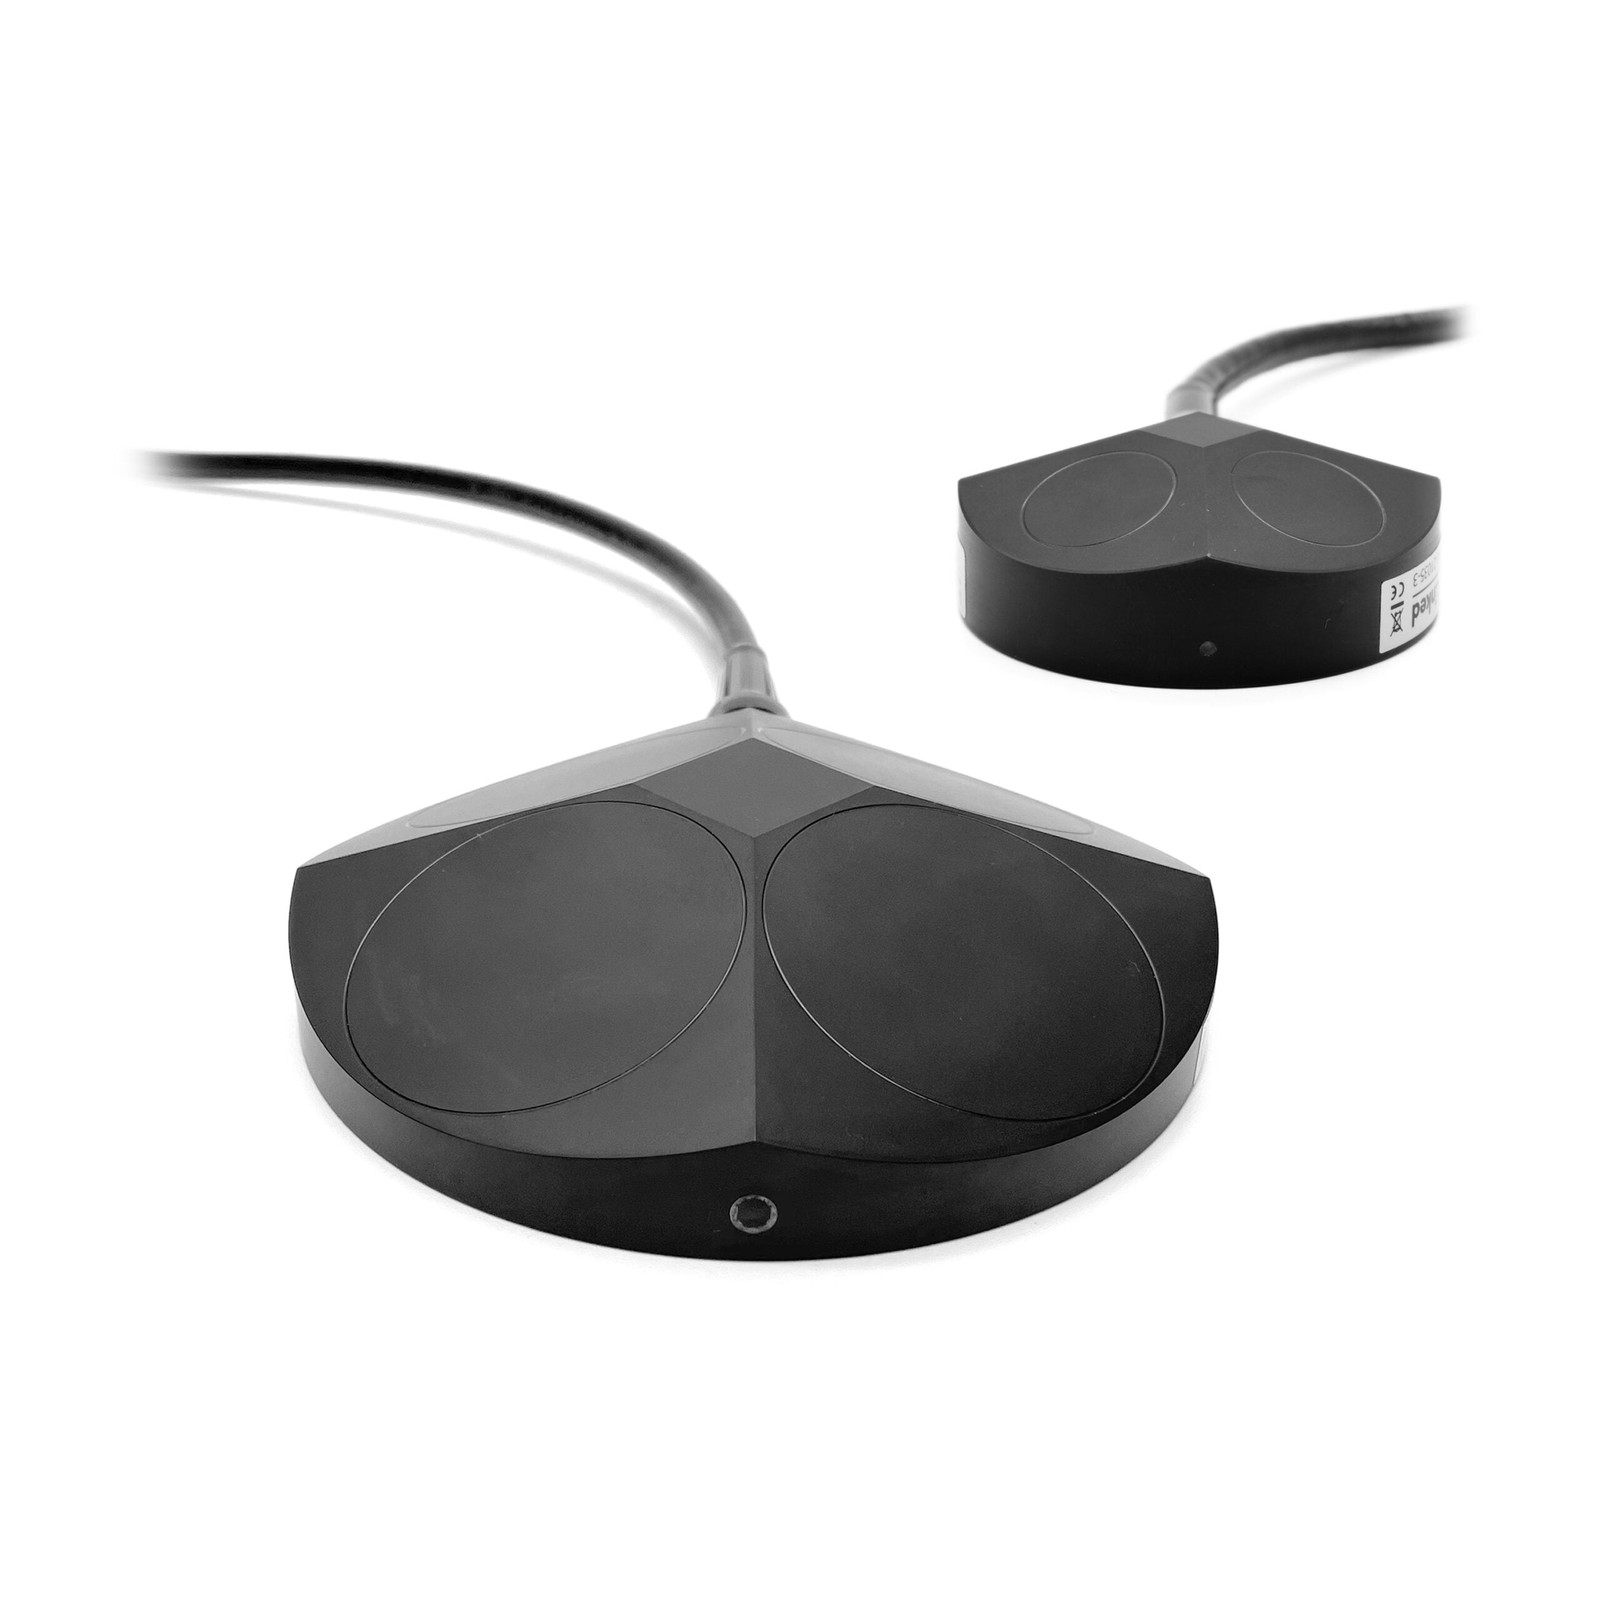
\includegraphics[height=2.3cm, keepaspectratio]{dvl_a50.jpg}\\
        \vspace{0.1em}
        \footnotesize\textbf{Water Linked DVL-A50}\\
        \scriptsize\textit{4 faisceaux Janus 1 MHz, 270 g dans l'eau}
      \end{center}
      \begin{center}
        \begin{tikzpicture}[scale=0.68]
          \draw[thick, fill=OceanMedium!20, rounded corners] (-1.8, 0.7) rectangle (1.8, 1.15);
          \node at (0, 0.92) {\tiny Châssis Sous-Marin};
          \draw[thick, fill=black!80] (-0.7, 0.25) rectangle (0.7, 0.7);
          \node[white] at (0, 0.48) {\tiny DVL};
          \draw[->, line width=1.1pt, OceanCyan] (-0.5, 0.25) -- (-1.4, -0.75);
          \draw[->, line width=1.1pt, OceanCyan] (0.5, 0.25) -- (1.4, -0.75);
          \draw[->, line width=1.1pt, OceanMedium] (-0.2, 0.25) -- (-0.5, -0.75);
          \draw[->, line width=1.1pt, OceanMedium] (0.2, 0.25) -- (0.5, -0.75);
          \draw[thick, fill=brown!30] (-2, -0.75) rectangle (2, -0.98);
          \node at (0, -0.86) {\tiny Fond marin (Bottom-Track)};
        \end{tikzpicture}
      \end{center}
    \end{column}
  \end{columns}
\end{frame}

\begin{frame}{2.12 Positionnement Acoustique Absolu : LBL vs USBL}
  \begin{table}[h]
    \centering
    \scriptsize
    \begin{tabularx}{\textwidth}{p{2.3cm} X X}
      \toprule
      \textbf{Critère} & \textbf{LBL (Long BaseLine)} & \textbf{USBL (Ultra-Short BaseLine)} \\
      \midrule
      \textbf{Principe géométrique} & Réseau de 3 à 4 balises transpondeuses ancrées et calibrées au fond marin autour de la zone & Antenne unique sous la coque / perche surface (matrice d'hydrophones espacés de quelques centimètres) \\
      \textbf{Méthode de calcul} & Triangulation / multilatération par temps de vol (ToF) aller-retour avec chaque balise & Distance par temps de vol (ToF) + \textbf{Gisement \& Site par déphasage} d'onde inter-éléments \\
      \textbf{Précision} & \succw{Centimétrique à décimétrique ($\pm 0.1\,\text{m}$)}, \textbf{indépendante de la profondeur} & Relative à la portée (\alertw{$0.2\%\text{--}1\%$ de la distance oblique}, ex: $\pm 1\,\text{m}$ à $100\,\text{m}$, $\pm 5\,\text{m}$ à $500\,\text{m}$) \\
      \textbf{Logistique \& Déploiement} & \alertw{Très lourde} : mouillage balises, calibration bathymétrique/GNSS par bateau, récupération en fin de manip & \succw{Ultra-légère} : perche sur semi-rigide ou ASV BlueBoat, zéro matériel au fond, suit le navire \\
      \textbf{Zone d'évolution} & Limitée au périmètre balisé ($1\text{--}2\,\text{km}^2$) & Mobile, suit le bateau support sans limite de zone \\
      \textbf{Sensibilité attitude} & Insensible aux mouvements de surface & \alertw{Critique} : nécessite une centrale d'attitude (MRU/IMU) en surface pour compenser roulis/tangage \\
      \bottomrule
    \end{tabularx}
  \end{table}
\end{frame}

\begin{frame}{2.12b Matériel Acoustique Réel : Balises LBL \& Transceivers USBL}
  \begin{columns}[c]
    \begin{column}{0.48\textwidth}
      \begin{center}
        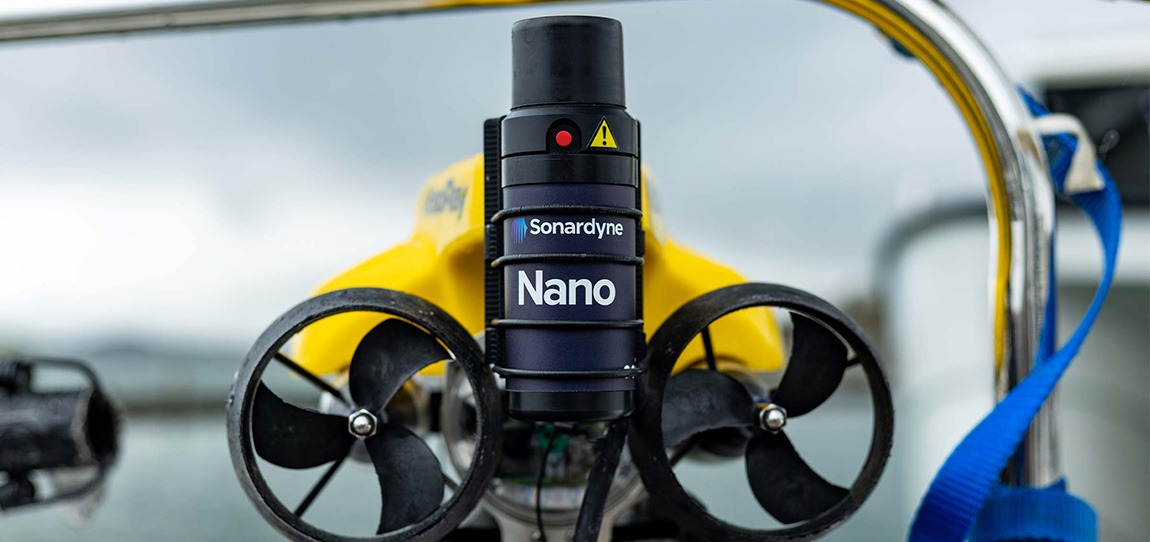
\includegraphics[height=1.8cm, keepaspectratio]{lbl_nano_transponder.jpg}
        \hspace{0.2cm}
        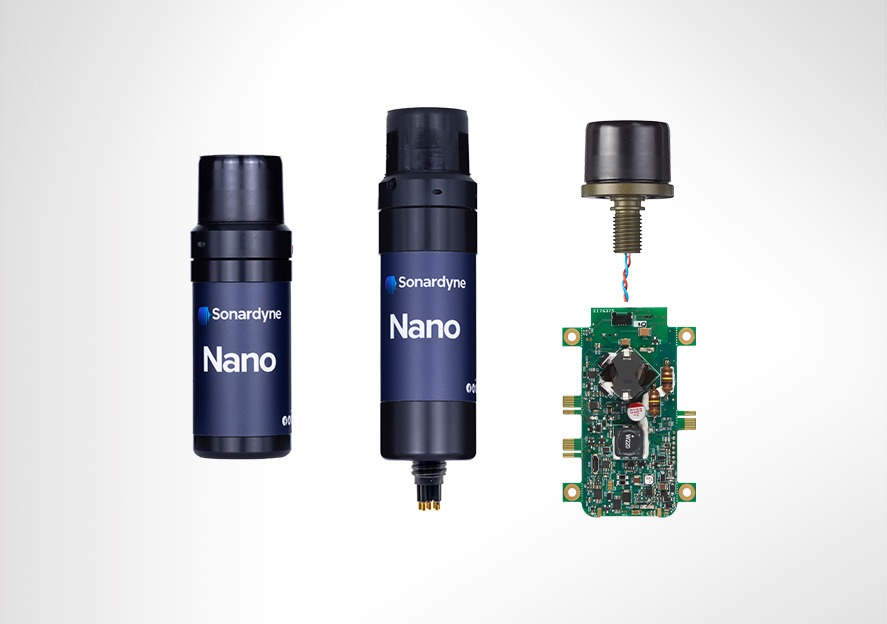
\includegraphics[height=1.8cm, keepaspectratio]{lbl_nano_beacon.jpg}\\
        \vspace{0.2em}
        \tech{Balise Transpondeuse LBL \& Ancrage}\\
        \tiny\textit{Réseau de fond fixe $\cdot$ Triangulation ToF centimétrique}
      \end{center}
      \scriptsize
      \begin{block}{Fonctionnement LBL Réel}
        Balise autonome sur batterie immergée au fond. Répond par un ping codé lorsqu'elle est interrogée par le robot.
      \end{block}
    \end{column}

    \begin{column}{0.48\textwidth}
      \begin{center}
        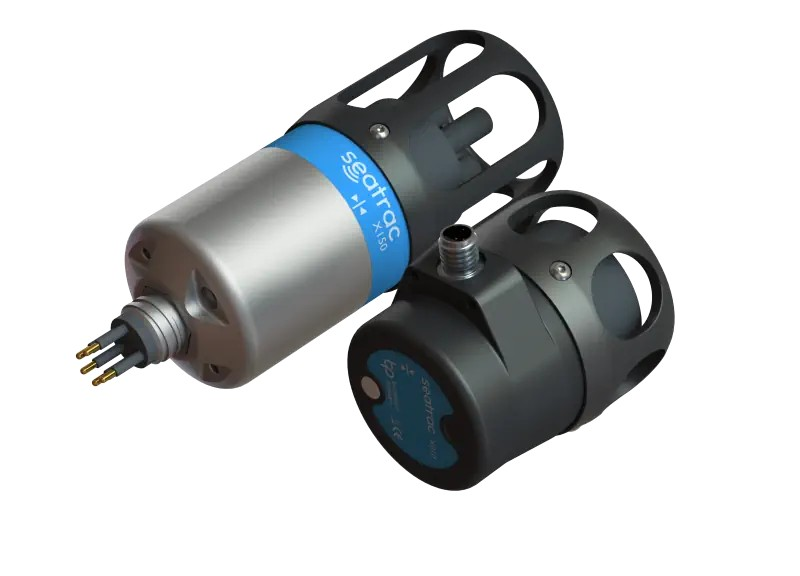
\includegraphics[height=1.8cm, keepaspectratio]{seatrac_usbl_photo.jpg}
        \hspace{0.2cm}
        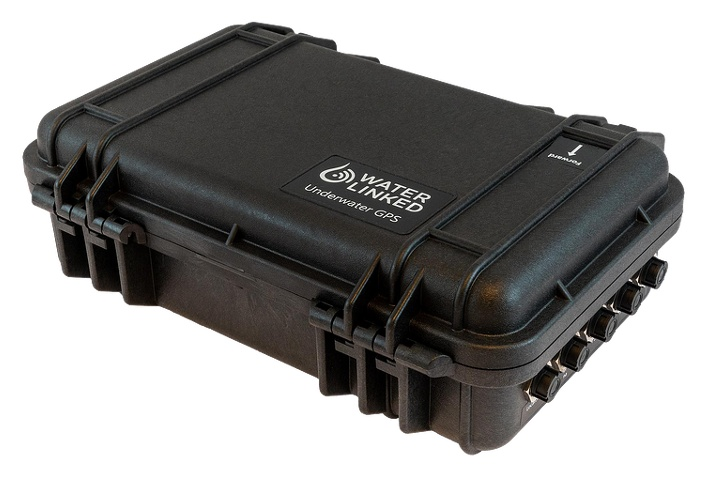
\includegraphics[height=1.8cm, keepaspectratio]{waterlinked_ugps.jpg}\\
        \vspace{0.2em}
        \succw{Antenne USBL Surface \& Transpondeur ROV}\\
        \tiny\textit{Systèmes SeaTrac X150 / Water Linked UGPS $\cdot$ Perche de surface}
      \end{center}
      \scriptsize
      \begin{block}{Fonctionnement USBL Réel}
        Matrice multi-hydrophones de surface mesurant les micro-déphasages d'angle d'arrivée ($\theta, \phi$) + temps de vol.
      \end{block}
    \end{column}
  \end{columns}
\end{frame}

\begin{frame}{2.13 Démocratisation USBL \& Télémétrie Acoustique ($\approx 5\,000$ €)}
  \begin{columns}[T, onlytextwidth]
    \begin{column}{0.44\textwidth}
      \begin{block}{\tech{1. Démocratisation des USBL}}
        \scriptsize
        \begin{itemize}\setlength{\itemsep}{2pt}\setlength{\parskip}{0pt}
          \item \textbf{Rupture de coût} : autrefois réservé à l'offshore ($>50\text{--}100\,\text{k€}$), désormais accessible aux labos (\succw{$\mathbf{\approx 5\text{--}8\,\text{k€}}$}, ex. \tech{Water Linked UGPS}, \tech{SeaTrac}).
          \item \textbf{Déploiement léger} : perche sur semi-rigide ou drone de surface ASV (\tech{BlueBoat}).
        \end{itemize}
      \end{block}

      \vspace{-0.15em}
      \begin{block}{\succw{2. Double Rôle : Position \& Télémesure}}
        \scriptsize
        \begin{itemize}\setlength{\itemsep}{2pt}\setlength{\parskip}{0pt}
          \item \textbf{Modem acoustique intégré} : données numériques modulées sur les pings (chirp / FSK, \textbf{quelques kbps}).
          \item \textbf{Voie montante} ($\uparrow$) : télémétrie vitale (profondeur Bar30, tension batterie, alarmes SOS / fuite).
          \item \textbf{Voie descendante} ($\downarrow$) : recalage fix GNSS absolu, ordres et waypoints de navigation.
        \end{itemize}
      \end{block}
    \end{column}

    \begin{column}{0.54\textwidth}
      \centering
      \begin{tikzpicture}[scale=0.92, every node/.style={transform shape}]
        % 1. Environnement : Ciel, Eau et Fond marin
        \fill[blue!4!white] (-4.0, 1.45) rectangle (4.0, 3.10);
        \fill[OceanCyan!8] (-4.0, -2.40) rectangle (4.0, 1.45);
        \fill[brown!22] (-4.0, -2.85) rectangle (4.0, -2.40);
        \draw[OceanMedium!40, line width=0.8pt, rounded corners=4pt] (-4.0, -2.85) rectangle (4.0, 3.10);

        % Ligne de surface (eau)
        \draw[OceanCyan, dashed, line width=0.9pt] (-4.0, 1.45) -- (4.0, 1.45);
        \node[OceanCyan!85!black, font=\fontsize{5}{6}\selectfont\bfseries, anchor=north west] at (-3.85, 1.35) {Surface (Eau de mer)};

        % Ligne de fond marin
        \draw[brown!60!black, thick] (-4.0, -2.40) -- (4.0, -2.40);
        \node[brown!80!black, font=\fontsize{5.5}{6.5}\selectfont\bfseries, anchor=west] at (-3.85, -2.62) {Fond marin (Bathymétrie)};
        \node[DarkSlate, font=\fontsize{4.8}{5.8}\selectfont, anchor=east] at (3.80, -2.62) {Portée : 50 à 500\,m};

        % 2. Cartouche 1 : Géoréférencement USBL (Dans le ciel / surface en haut à gauche)
        \node[anchor=north west, fill=white, fill opacity=0.96, text opacity=1, draw=OceanCyan, line width=0.8pt, rounded corners=3pt, inner sep=3pt, drop shadow={opacity=0.08}] at (-3.9, 3.02) {%
          \begin{minipage}{4.0cm}
            \textcolor{OceanDeep}{\textbf{\scriptsize 1. Géoréférencement USBL}}\\[1pt]
            \centering
            {\scriptsize\succw{$\vec{X}_{\text{AUV}} = \vec{X}_{\text{GNSS}} + \mathbf{R}_{\text{bateau}} \cdot \vec{P}_{\text{USBL}}$}}\\[2pt]
            \raggedright\fontsize{5}{6}\selectfont
            $\bullet$ \textbf{Distance $D$} : temps de vol aller-retour ($\Delta t$)\\
            $\bullet$ \textbf{Direction $(\theta, \psi)$} : déphasage hydrophones\\
            $\implies$ Fix GNSS absolu injecté dans l'AUV
          \end{minipage}
        };

        % 3. Bateau support / ASV de surface (BlueBoat)
        \draw[thick, fill=white, draw=OceanDeep, rounded corners=2pt] (0.8, 1.4) -- (1.2, 2.15) -- (3.8, 2.15) -- (3.4, 1.4) -- cycle;
        \node[font=\scriptsize\bfseries, text=OceanDeep] at (2.4, 1.78) {ASV Surface};

        % Mât et antenne GNSS RTK
        \draw[line width=1.4pt, DarkSlate] (3.2, 2.15) -- (3.2, 2.75);
        \fill[OceanDeep] (3.2, 2.75) circle (2.8pt);
        \draw[OceanDeep, line width=0.6pt] (3.06, 2.82) arc[start angle=150, end angle=30, radius=0.16];
        \draw[OceanDeep, line width=0.6pt] (2.96, 2.89) arc[start angle=150, end angle=30, radius=0.27];
        \node[anchor=south east, font=\tiny\bfseries, text=OceanDeep] at (3.05, 2.5) {GNSS};
        \node[anchor=south east, font=\fontsize{5}{6}\selectfont, text=OceanMedium] at (3.05, 2.22) {Fix $\vec{X}_{\text{surf}}$};

        % Perche rigide et Antenne USBL immergée
        \draw[line width=2.6pt, DarkSlate] (1.35, 1.4) -- (1.35, 0.42);
        \draw[line width=0.8pt, fill=DarkSlate, rounded corners=1pt] (1.10, 0.30) rectangle (1.60, 0.44);
        \fill[OceanCoral] (1.35, 0.26) circle (4.2pt);
        \fill[white] (1.23, 0.26) circle (1pt);
        \fill[white] (1.47, 0.26) circle (1pt);
        \node[anchor=west, font=\tiny\bfseries, text=OceanCoral] at (1.75, 0.40) {Tête USBL};
        \node[anchor=west, font=\fontsize{4.8}{5.8}\selectfont, text=DarkSlate] at (1.75, 0.20) {(4 hydrophones)};

        % 4. Véhicule sous-marin (AUV / BlueROV2)
        \draw[line width=1.1pt, fill=OceanMedium!15, draw=OceanDeep, rounded corners=4pt] (-3.5, -2.25) rectangle (-1.5, -1.65);
        \node[font=\scriptsize\bfseries, text=OceanDeep] at (-2.5, -1.95) {AUV};
        % Propulseurs
        \fill[DarkSlate] (-3.68, -2.18) rectangle (-3.5, -2.04);
        \fill[DarkSlate] (-3.68, -1.86) rectangle (-3.5, -1.72);
        % Capteur Bar30
        \fill[OceanCyan] (-1.5, -1.95) circle (2.2pt);
        \node[anchor=west, font=\fontsize{4.8}{5.8}\selectfont, text=OceanMedium] at (-1.45, -1.95) {Bar30 ($z$)};
        % Transpondeur acoustique
        \draw[line width=1pt, fill=DarkSlate] (-2.25, -1.65) rectangle (-1.95, -1.40);
        \fill[OceanCoral] (-2.1, -1.33) circle (3.5pt);
        \node[anchor=south east, font=\tiny\bfseries, text=OceanCoral] at (-2.2, -1.35) {Transpondeur};

        % 5. Fronts d'ondes acoustiques stylisés
        \draw[OceanCyan!30, line width=1pt] (0.95, 0.05) arc[start angle=195, end angle=235, radius=0.6];
        \draw[OceanCyan!30, line width=1.1pt] (0.45, -0.18) arc[start angle=195, end angle=235, radius=1.2];
        \draw[OceanCyan!30, line width=1.2pt] (-0.05, -0.42) arc[start angle=195, end angle=235, radius=1.8];

        % 6. Faisceaux acoustiques (Pings & Modem)
        % Faisceau USBL
        \draw[{Latex[length=2.2mm]}-{Latex[length=2.2mm]}, line width=2.0pt, OceanCyan] (1.10, 0.12) -- (-1.80, -1.22);
        \node[pos=0.44, sloped, above=3pt, fill=white, fill opacity=0.94, text opacity=1, draw=OceanCyan!70, rounded corners=2pt, inner sep=1.6pt, font=\fontsize{5.2}{6.2}\selectfont\bfseries, text=OceanMedium] {1. Pings USBL (ToF + Déphasage)};

        % Faisceau Modem
        \draw[{Latex[length=1.8mm]}-{Latex[length=1.8mm]}, line width=1.6pt, OceanGreen, dashed] (1.25, -0.06) -- (-1.65, -1.38);
        \node[pos=0.44, sloped, below=3pt, fill=white, fill opacity=0.94, text opacity=1, draw=OceanGreen!70, rounded corners=2pt, inner sep=1.6pt, font=\fontsize{5.2}{6.2}\selectfont\bfseries, text=OceanGreen!80!black] {2. Modem Acoustique ($\uparrow\downarrow$ Données \& Ordres)};

        % 7. Cartouche 2 : Modem Acoustique (Coin inférieur droit)
        \node[anchor=north west, fill=white, fill opacity=0.96, text opacity=1, draw=OceanGreen, line width=0.8pt, rounded corners=3pt, inner sep=3pt, drop shadow={opacity=0.08}] at (0.5, -0.60) {%
          \begin{minipage}{3.3cm}
            \textcolor{OceanDeep}{\textbf{\scriptsize 2. Liaison Acoustique Sans Fil}}\\[1pt]
            \fontsize{5}{6}\selectfont
            \succw{$\blacktriangledown$} \textbf{Descendant (Surface $\rightarrow$ Robot)} :\\
            \quad $\cdot$ Recalage Kalman (fix GNSS absolu)\\
            \quad $\cdot$ Consignes, waypoints, arrêt SOS\\[1.5pt]
            \alertw{$\blacktriangle$} \textbf{Montant (Robot $\rightarrow$ Surface)} :\\
            \quad $\cdot$ Profondeur Bar30 ($z$), tension Li-Ion,\\
            \quad $\cdot$ Alarmes SOS \& détection de fuite
          \end{minipage}
        };
      \end{tikzpicture}
    \end{column}
  \end{columns}
\end{frame}

\begin{frame}{2.14 Propagation Acoustique \& Pièges de Terrain}
  \begin{columns}[T]
    \begin{column}{0.49\textwidth}
      \begin{block}{\tech{1. Célérité $c(z)$ \& Réfraction (Loi de Snell)}}
        \scriptsize
        \begin{itemize}
          \item La célérité $c(S,T,P) \approx 1450\text{--}1540\,\text{m/s}$ varie selon la thermocline et la pycnocline.
          \item Réfraction : les rayons acoustiques se courbent systématiquement vers les couches où le son est plus lent ($\frac{\cos\theta}{c} = \text{cte}$).
          \item \alertw{Création de zones d'ombre} (zones de silence où aucun ping ne passe) et erreurs de distance si $c(z)$ n'est pas mesuré par sonde CTD/SVP.
        \end{itemize}
      \end{block}

      \begin{block}{\alertw{2. Multi-trajets}}
        \scriptsize
        \begin{itemize}
          \item Réflexions parasites sur l'interface air-eau et sur le fond marin.
          \item Arrivée d'échos multiples déphasés qui brouillent le signal direct : critique par \textbf{petits fonds ($<15\,\text{m}$)}, bassins et zones portuaires.
        \end{itemize}
      \end{block}
    \end{column}

    \begin{column}{0.49\textwidth}
      \begin{block}{\alertw{3. Masquages Géométriques}}
        \scriptsize
        \begin{itemize}
          \item \textbf{Relief sous-marin} : dômes rocheux, canyons, surplombs, épaves et piliers de quai qui coupent la ligne de visée acoustique (*Line-of-Sight*).
          \item \textbf{Vecteur porteur} : masquage par la coque du bateau ou l'ombilical.
        \end{itemize}
      \end{block}

      \begin{block}{\succw{4. Bruits Ambiants \& Atténuation}}
        \scriptsize
        \begin{itemize}
          \item \textbf{Aération de surface} : bulles d'air sous la coque formant un écran opaque aux ondes sonores.
          \item \textbf{Cavitation \& moteurs} : bruit des hélices à forte poussée couvrant les signaux de faible amplitude.
          \item \textbf{Atténuation avec la fréquence} : haute fréquence ($>100\,\text{kHz}$) = portée courte ($<100\,\text{m}$).
        \end{itemize}
      \end{block}
    \end{column}
  \end{columns}
\end{frame}

% ==============================================================================
% 03_comms_autonomie.tex - Module 3 (13h30 - 15h00)
% Particularité des communications et de la programmation d'un drone sous-marin
% Pratique : Fathom-X, BlueOS (Docker), Cockpit, MAVLink et intégration ROS 2
% ==============================================================================

\section{Module 3 : Communications, BlueOS, Cockpit \& Intégration ROS 2}

\begin{frame}{3.1 Le Défi de la Transmission Fil de Surface : Fathom-X}
  \begin{columns}[c]
    \begin{column}{0.54\textwidth}
      \textbf{Comment faire passer 100 Mbps sur 300 m ?}
      \scriptsize
      \begin{itemize}
        \item Un câble réseau Ethernet standard (Cat5e/Cat6) est trop rigide et atténue au-delà de $100\,\text{m}$.
        \item \succw{La solution : HomePlug AV} (courant porteur CPL adapté).
        \item La carte \tech{Fathom-X} (Qualcomm AR7420) convertit l'Ethernet en signal différentiel robuste sur une \textbf{unique paire de fils torsadés non blindés}.
        \item Câble \tech{Fathom Tether} : diamètre fin ($7.6\,\text{mm}$), densité neutre (flotte sans couler ni tirer le ROV), résistance de $150\,\text{kgf}$.
      \end{itemize}

      \vspace{0.3em}
      \begin{block}{Débit \& Télémétrie}
        \scriptsize
        $\mathbf{100\,\text{Mbps}}$ bidirectionnel : flux vidéo Full HD H.264 temps réel ($<120\,\text{ms}$) + flux MAVLink + capteurs scientifiques.
      \end{block}
    \end{column}

    \begin{column}{0.44\textwidth}
      \begin{center}
        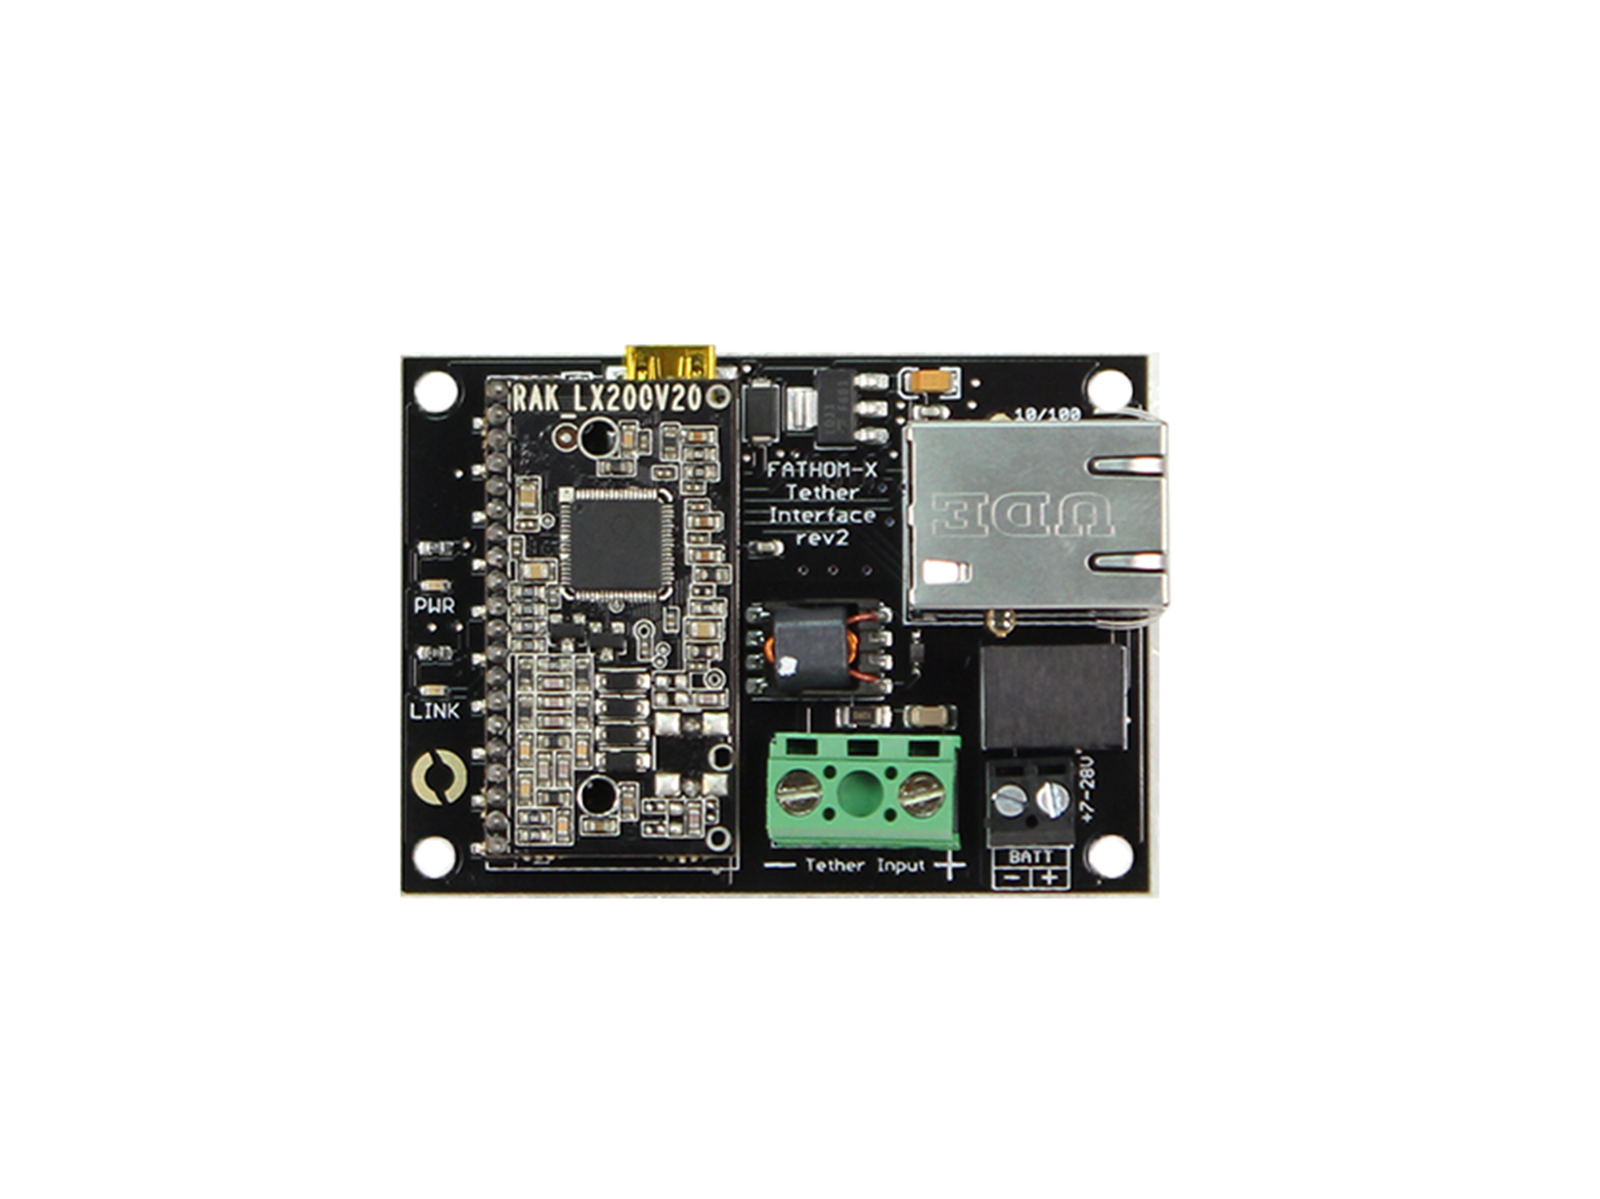
\includegraphics[height=1.8cm, keepaspectratio]{fathom_x.png}
        \hspace{0.2cm}
        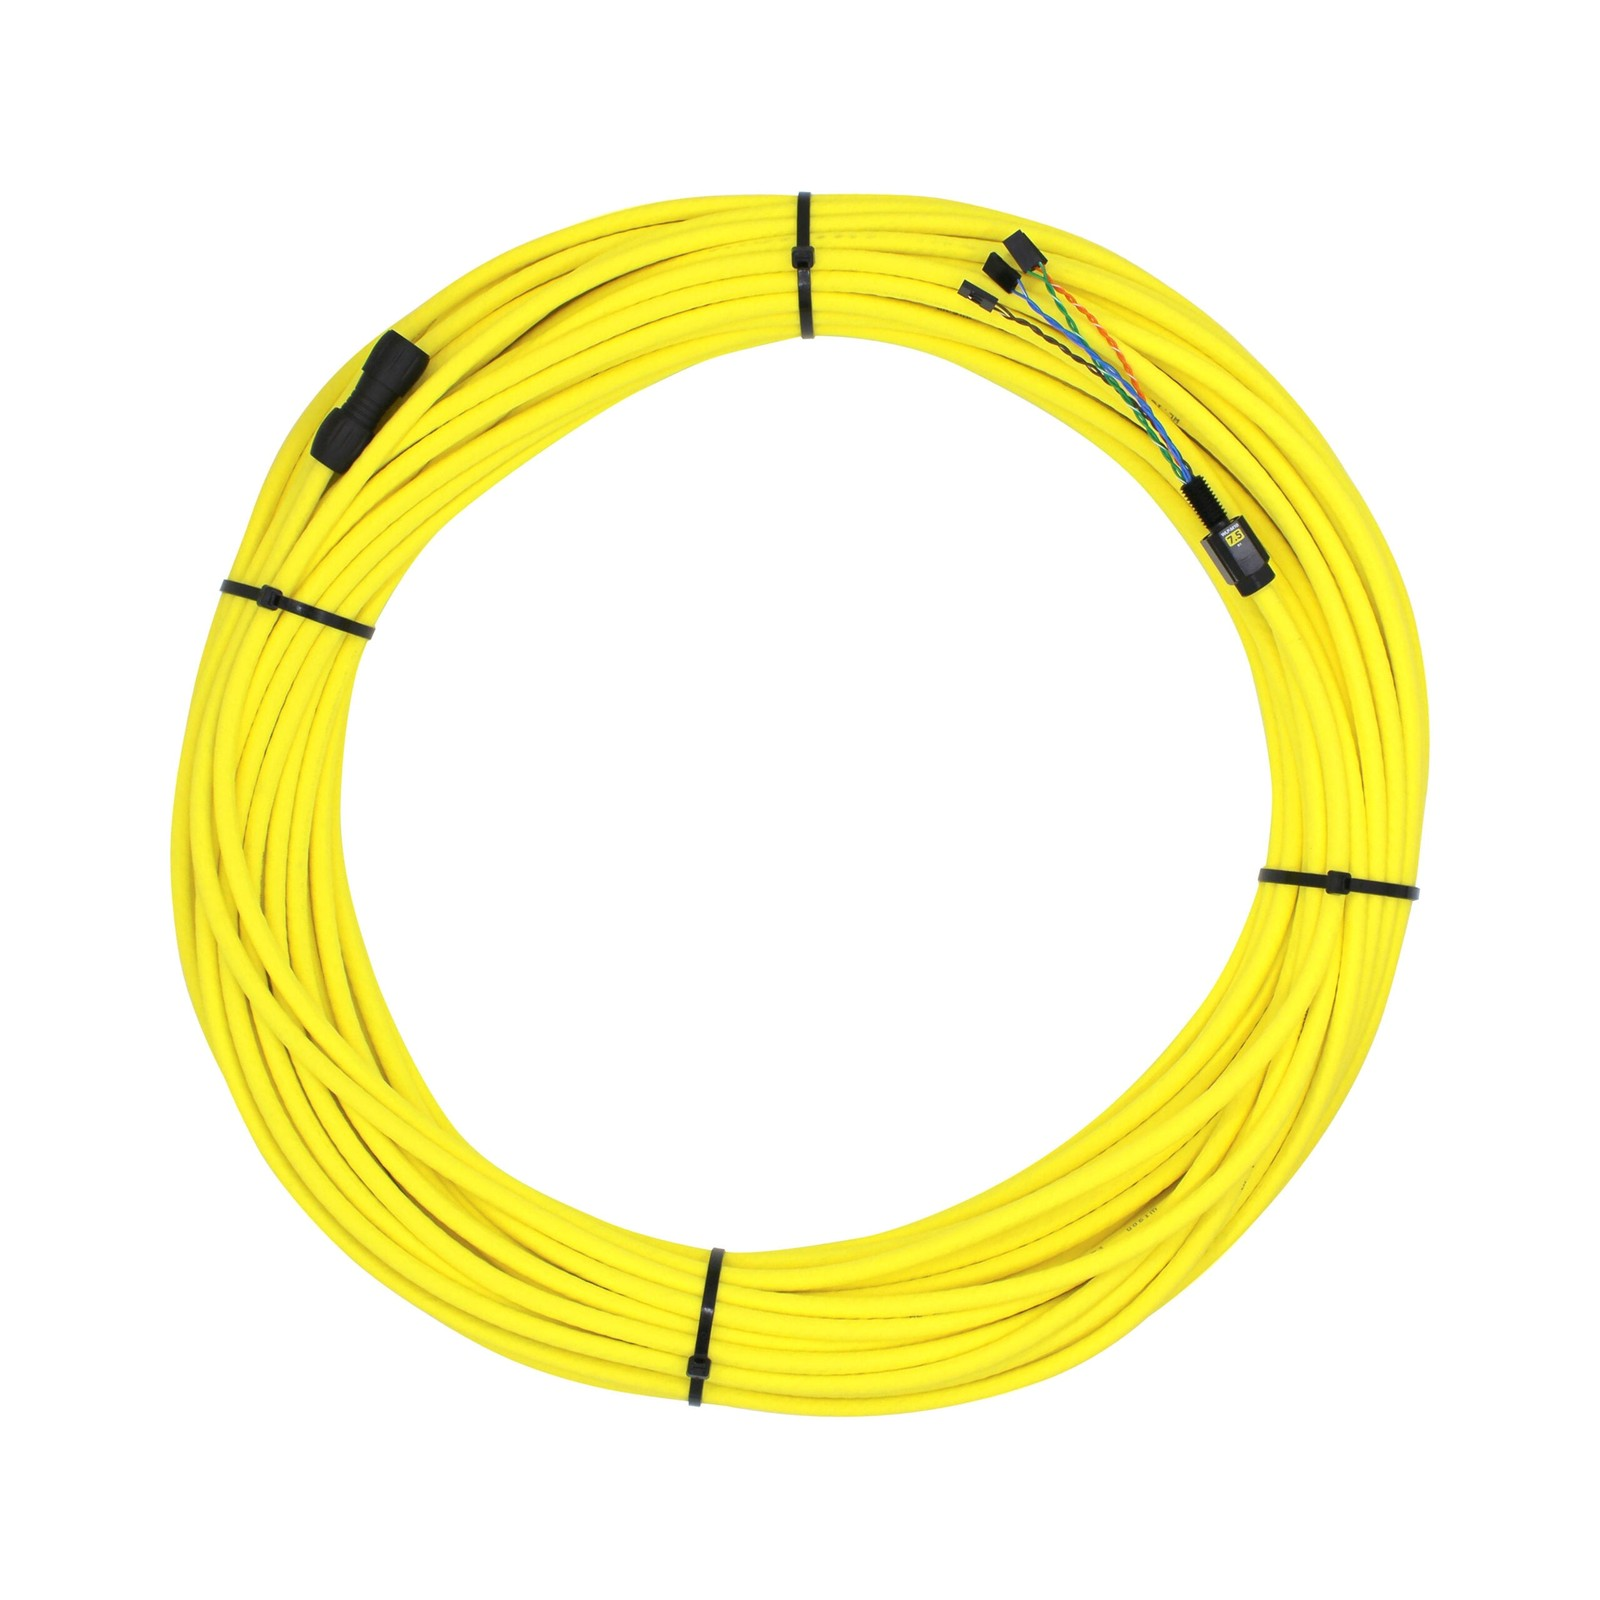
\includegraphics[height=1.8cm, keepaspectratio]{fathom_tether.jpg}\\
        \vspace{0.1em}
        \scriptsize\textbf{Carte Fathom-X} \hspace{0.6cm} \textbf{Ombilical Fathom}\\
        \tiny\textit{CPL HomePlug AV} \hspace{0.5cm} \textit{Flottabilité neutre 300 m}
      \end{center}
      
      \begin{center}
        \begin{tikzpicture}[scale=0.72, every node/.style={transform shape}]
          \node[draw=OceanDeep, fill=OceanDeep!20, rounded corners] (rpi) at (-2,1.2) {\scriptsize RPi 4/5};
          \node[draw=OceanMedium, fill=OceanMedium!20, rounded corners] (fx1) at (-2,0) {\scriptsize Fathom-X};
          \node[draw=OceanMedium, fill=OceanMedium!20, rounded corners] (fx2) at (2,0) {\scriptsize Fathom-X};
          \node[draw=OceanGreen, fill=OceanGreen!20, rounded corners] (pc) at (2,1.2) {\scriptsize PC Surface};
          \draw[<->, thick] (rpi) -- (fx1);
          \draw[<->, line width=1.5pt, OceanCoral] (fx1) -- (fx2) node[midway, above] {\tiny 1 paire 300m};
          \draw[<->, thick] (fx2) -- (pc);
        \end{tikzpicture}
      \end{center}
    \end{column}
  \end{columns}
\end{frame}

\begin{frame}{3.1b Variantes d'Ombilicaux \& Gestion du Câble : Enrouleur de Pont}
  \begin{columns}[T]
    \begin{column}{0.48\textwidth}
      \begin{block}{\tech{Types de Câbles Ombilicaux (Tethers)}}
        \scriptsize
        \begin{itemize}
          \item \textbf{Tether 2 brins (Fathom Standard / Slim)} :
            \begin{itemize}\tiny
              \item 1 paire torsadée Fathom-X ($100\,\text{Mbps}$) + brin central Kevlar.
              \item $\varnothing 7.6\,\text{mm}$ (standard, $150\,\text{kgf}$) vs $\varnothing 4.0\,\text{mm}$ (Slim, traînée $\div 2$).
            \end{itemize}
          \item \textbf{Tether 8 brins (Gigabit High-Bandwidth)} :
            \begin{itemize}\tiny
              \item 4 paires blindées ($1000\,\text{Mbps}$) pour flux 4K \& sonars lourds.
            \end{itemize}
        \end{itemize}
      \end{block}

      \vspace{0.2em}
      \begin{center}
        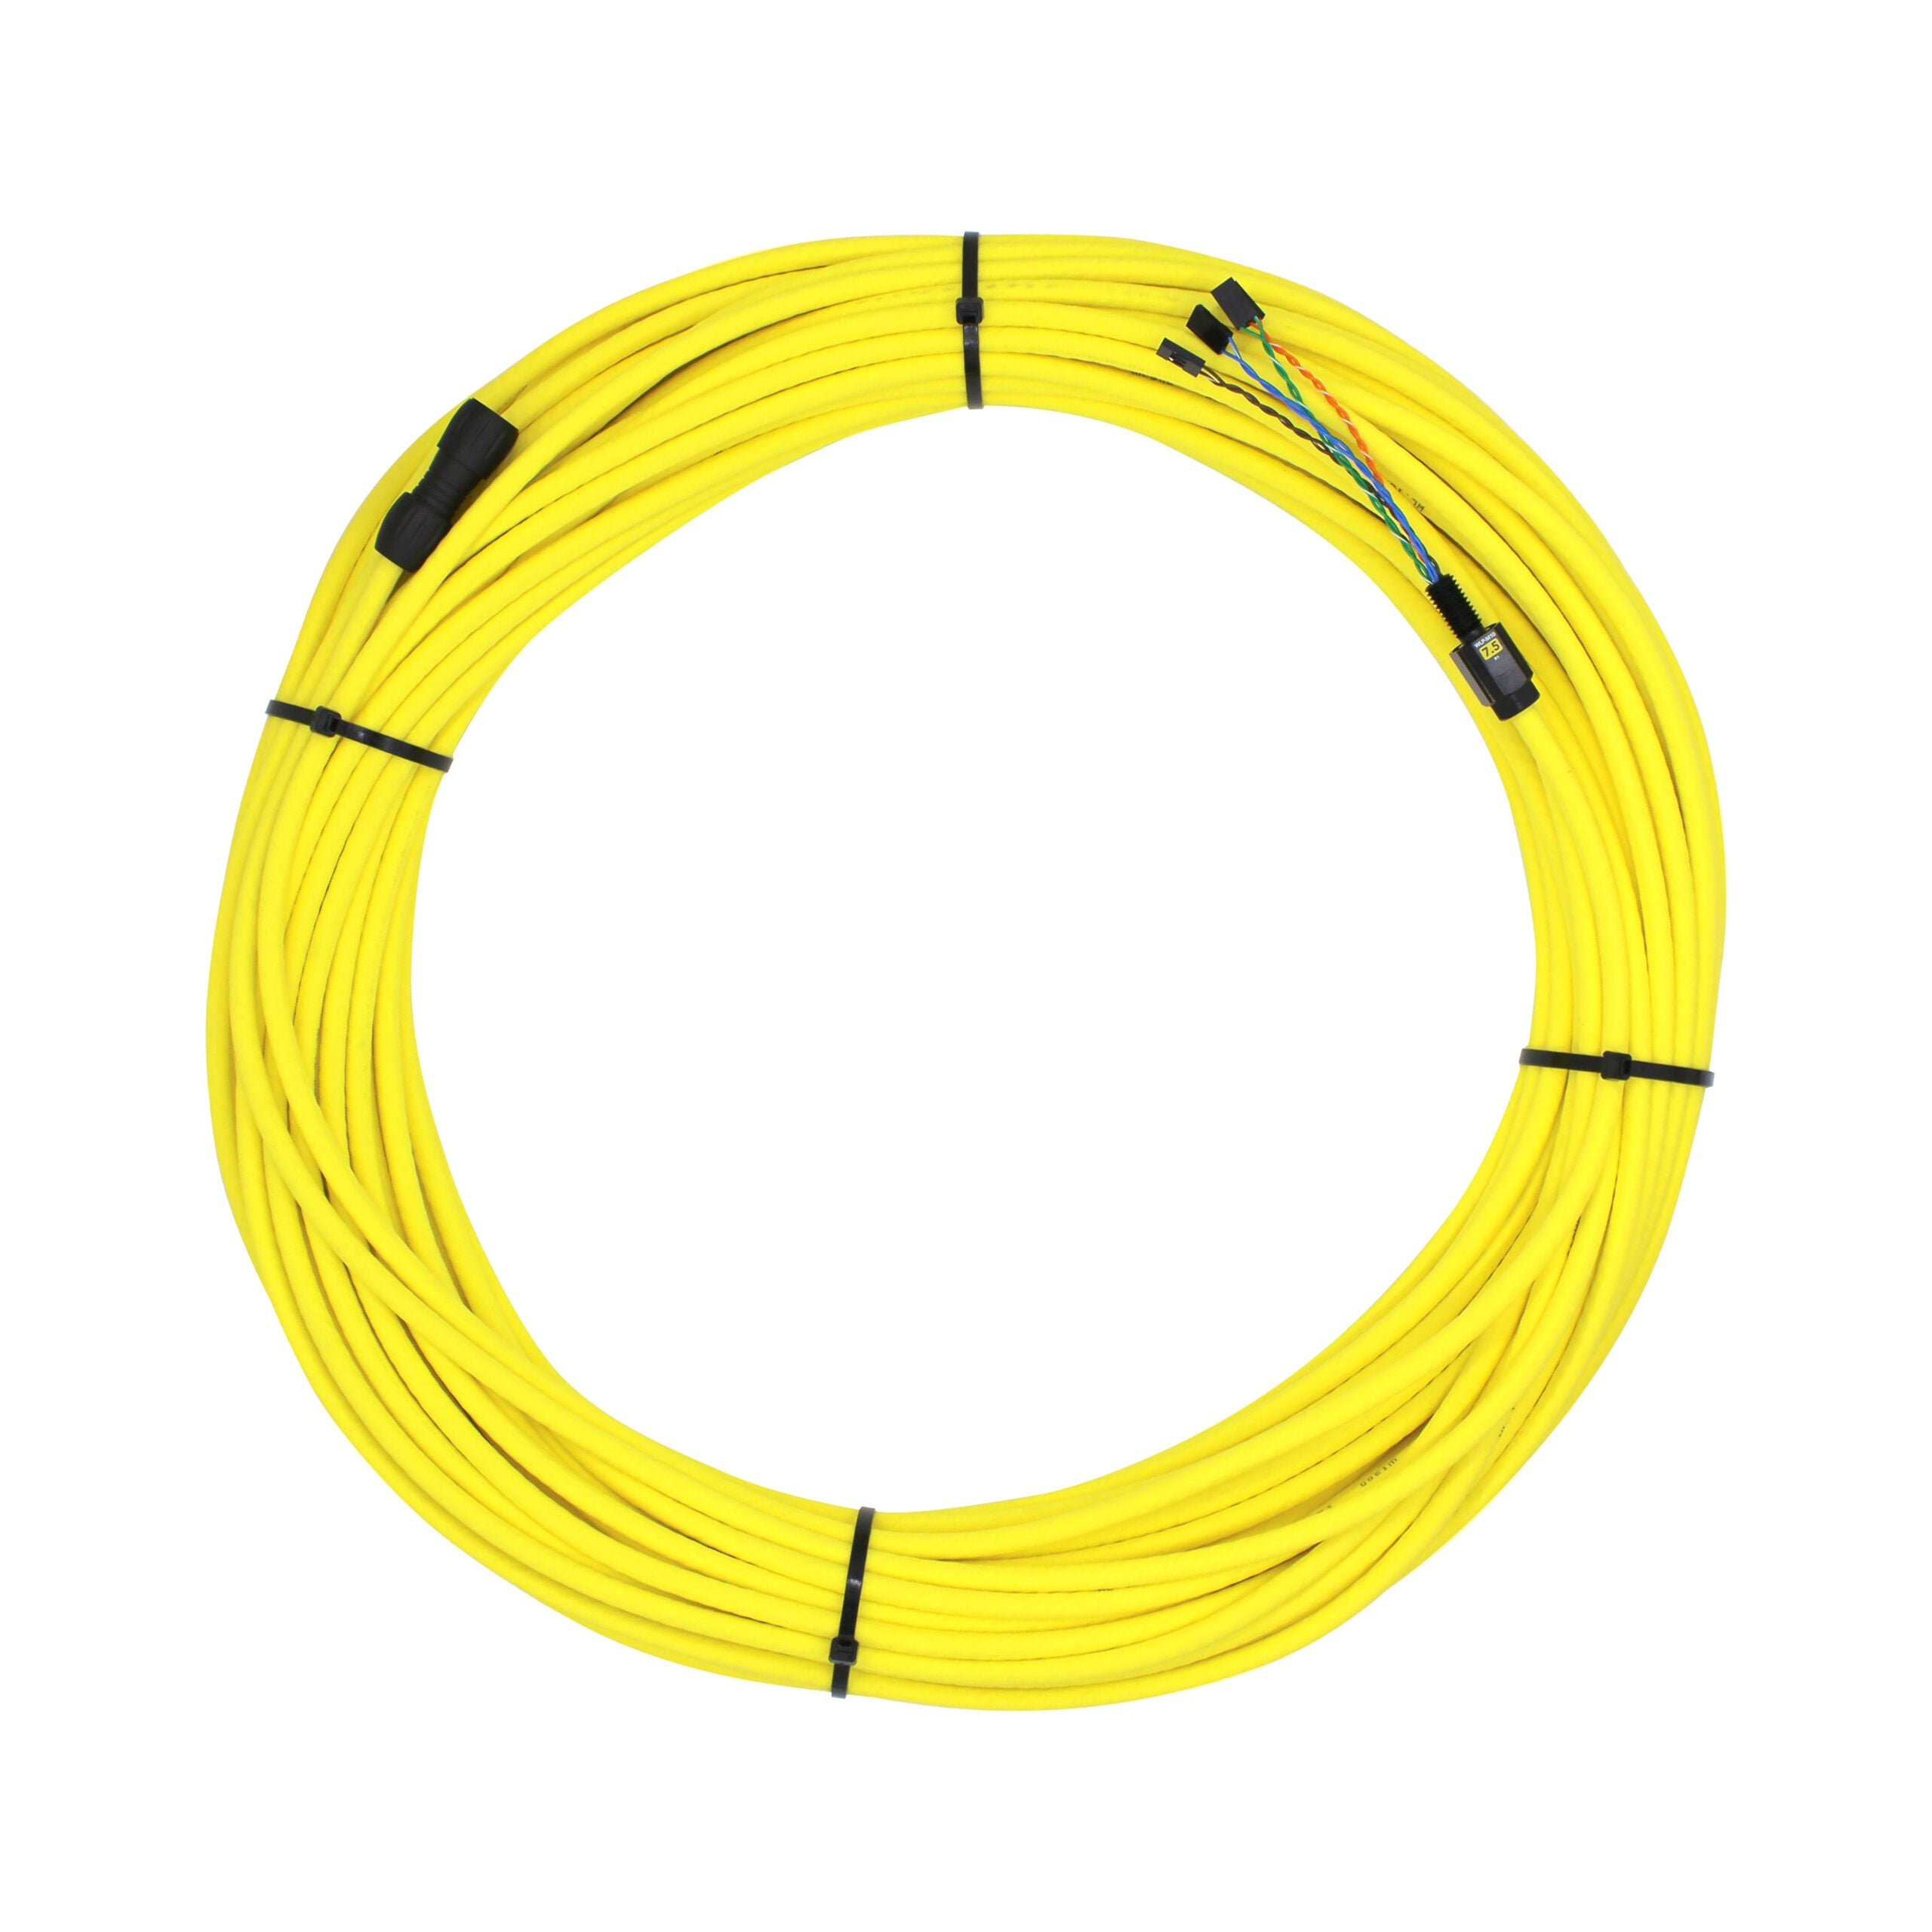
\includegraphics[height=1.4cm, keepaspectratio]{tether_standard_photo.jpg}
        \hspace{0.2cm}
        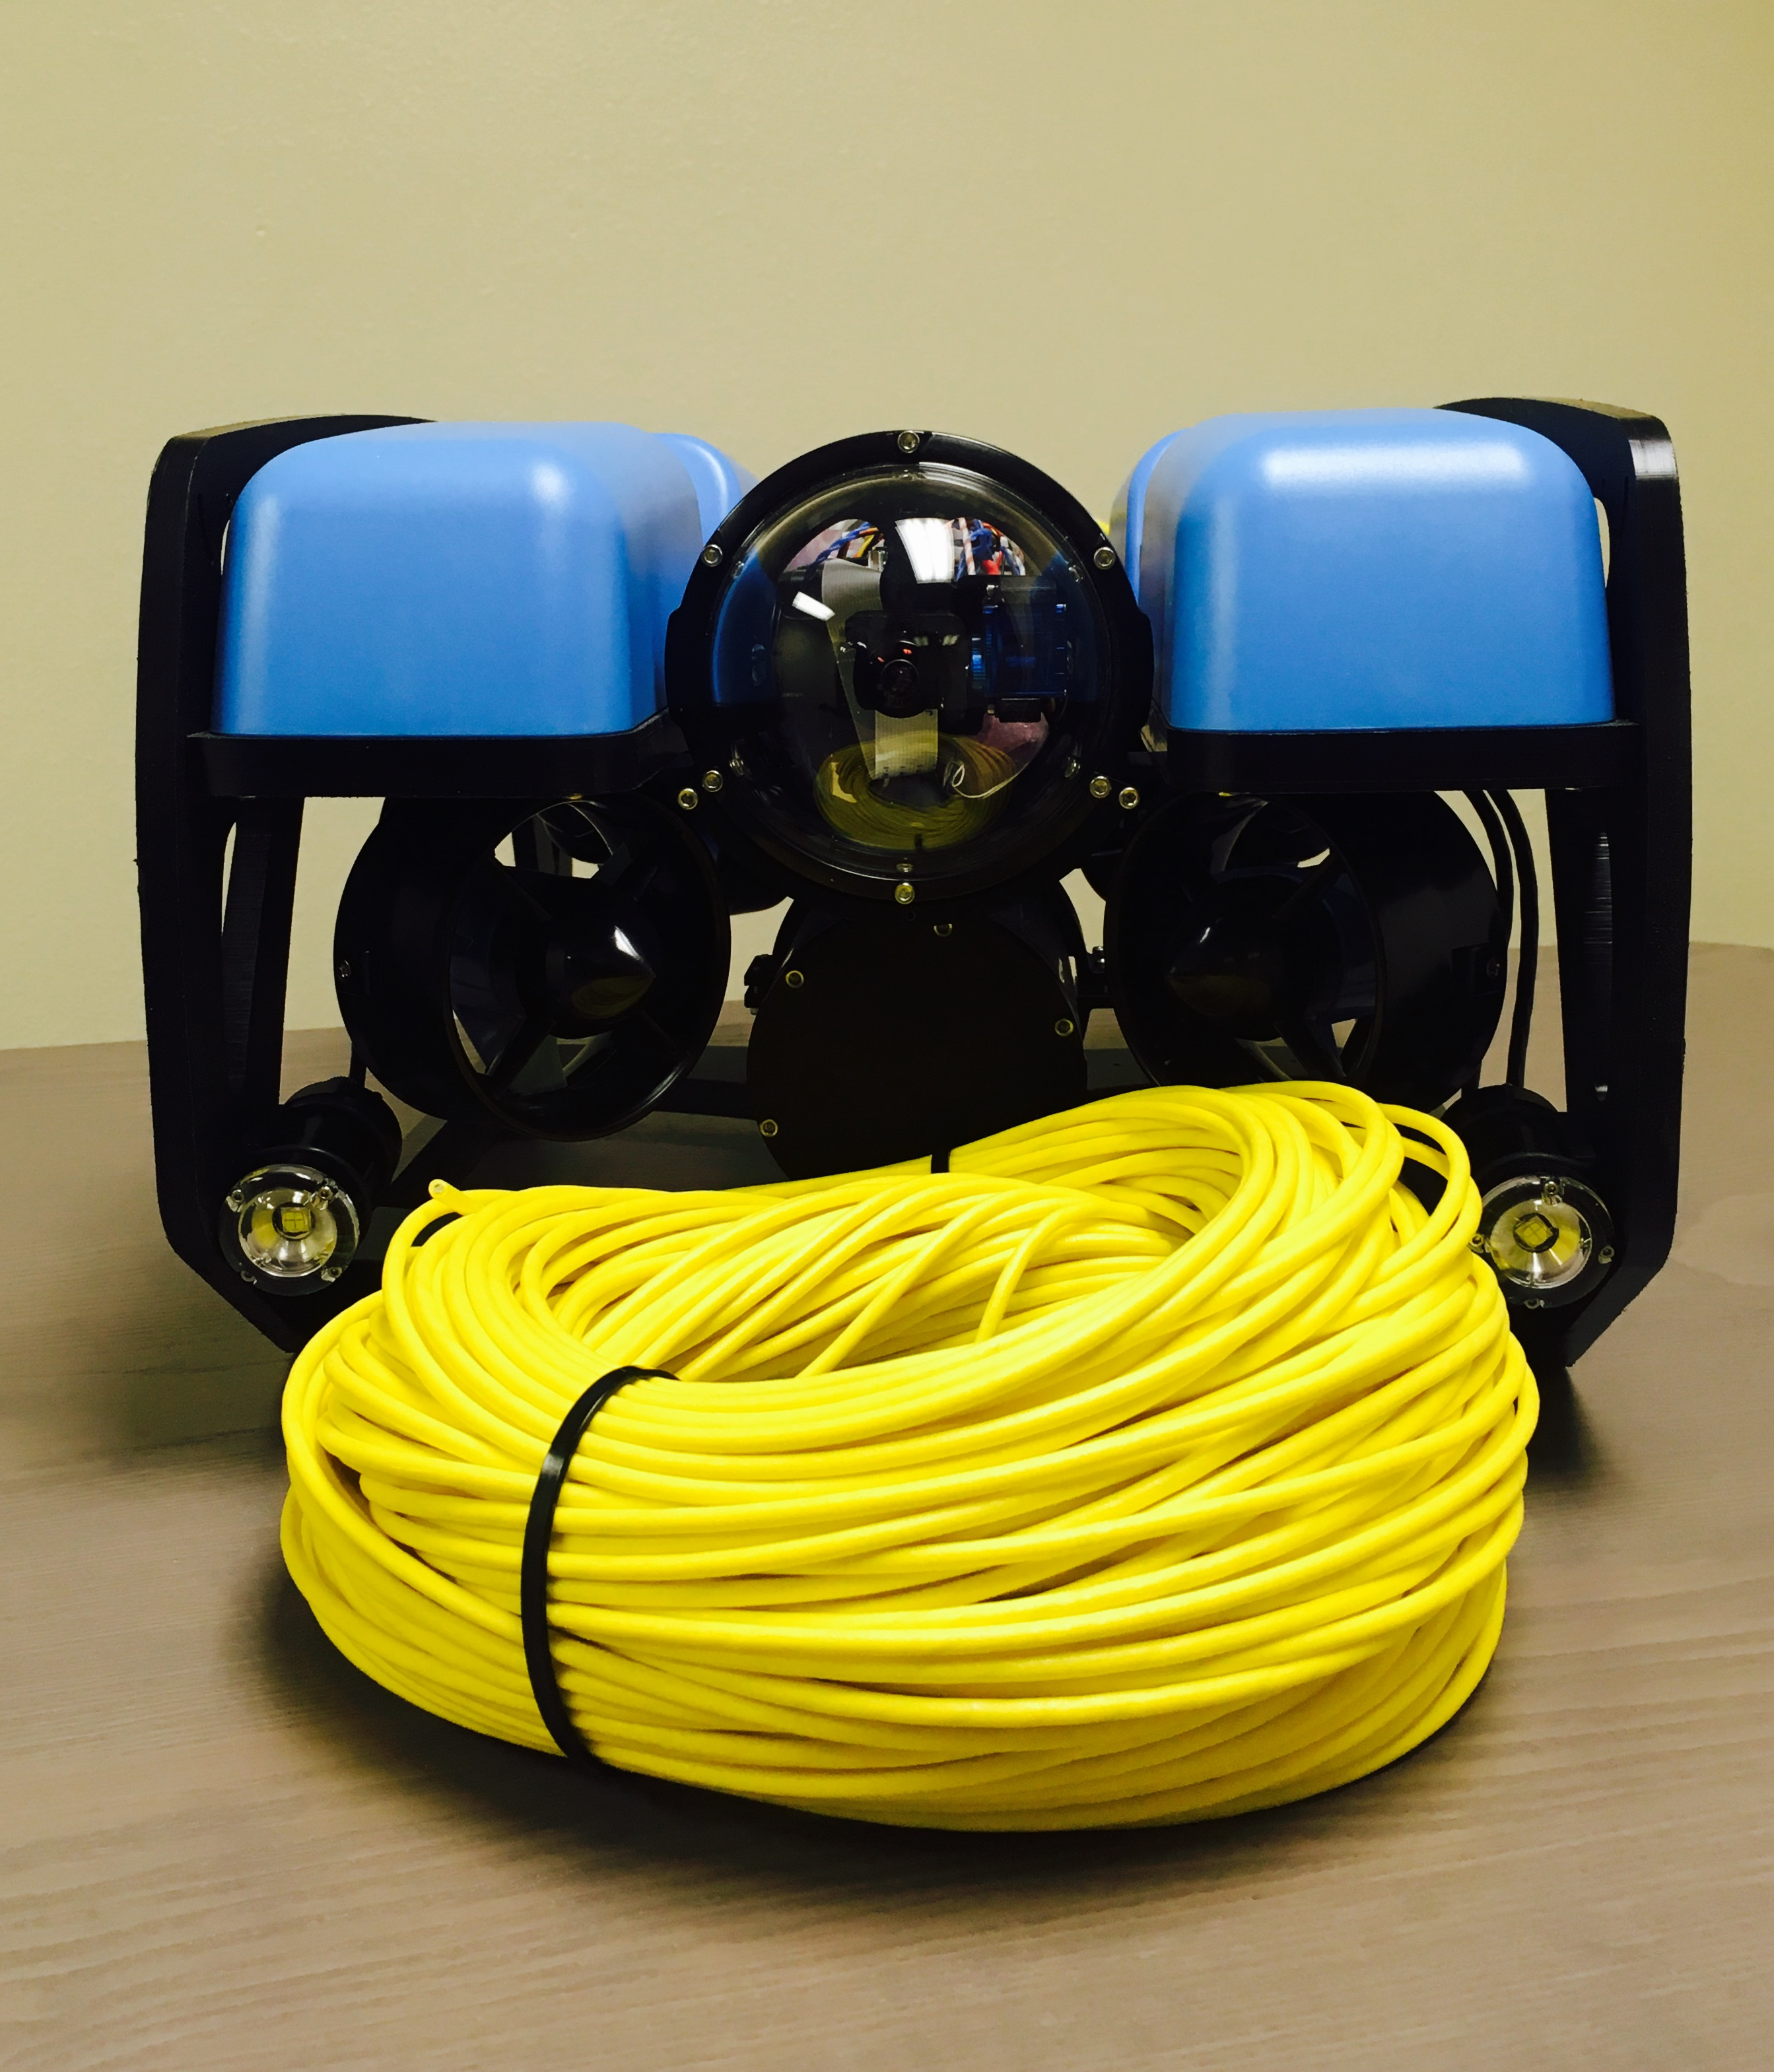
\includegraphics[height=1.4cm, keepaspectratio]{tether_slim_photo.jpg}\\
        \vspace{0.1em}
        \tiny\textbf{Ombilical Standard ($\varnothing 7.6\,\text{mm}$)} \hspace{0.3cm} \textbf{Ombilical Slim ($\varnothing 4.0\,\text{mm}$)}
      \end{center}
    \end{column}

    \begin{column}{0.50\textwidth}
      \begin{block}{\succw{L'Enrouleur de Pont avec Collecteur Tournant (*Slip Ring*)}}
        \scriptsize
        \begin{itemize}
          \item \textbf{Gestion des $300\,\text{m}$ de câble} : déroulage et virage sous tension sans vrille.
          \item \textbf{Joint tournant électro-optique / slip ring} : transfert continu des signaux haute fréquence ($100\text{--}1000\,\text{Mbps}$) pendant la rotation du touret.
        \end{itemize}
      \end{block}

      \vspace{0.2em}
      \begin{center}
        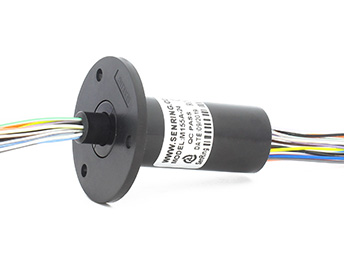
\includegraphics[height=1.4cm, keepaspectratio]{slip_ring.jpg}
        \hspace{0.3cm}
        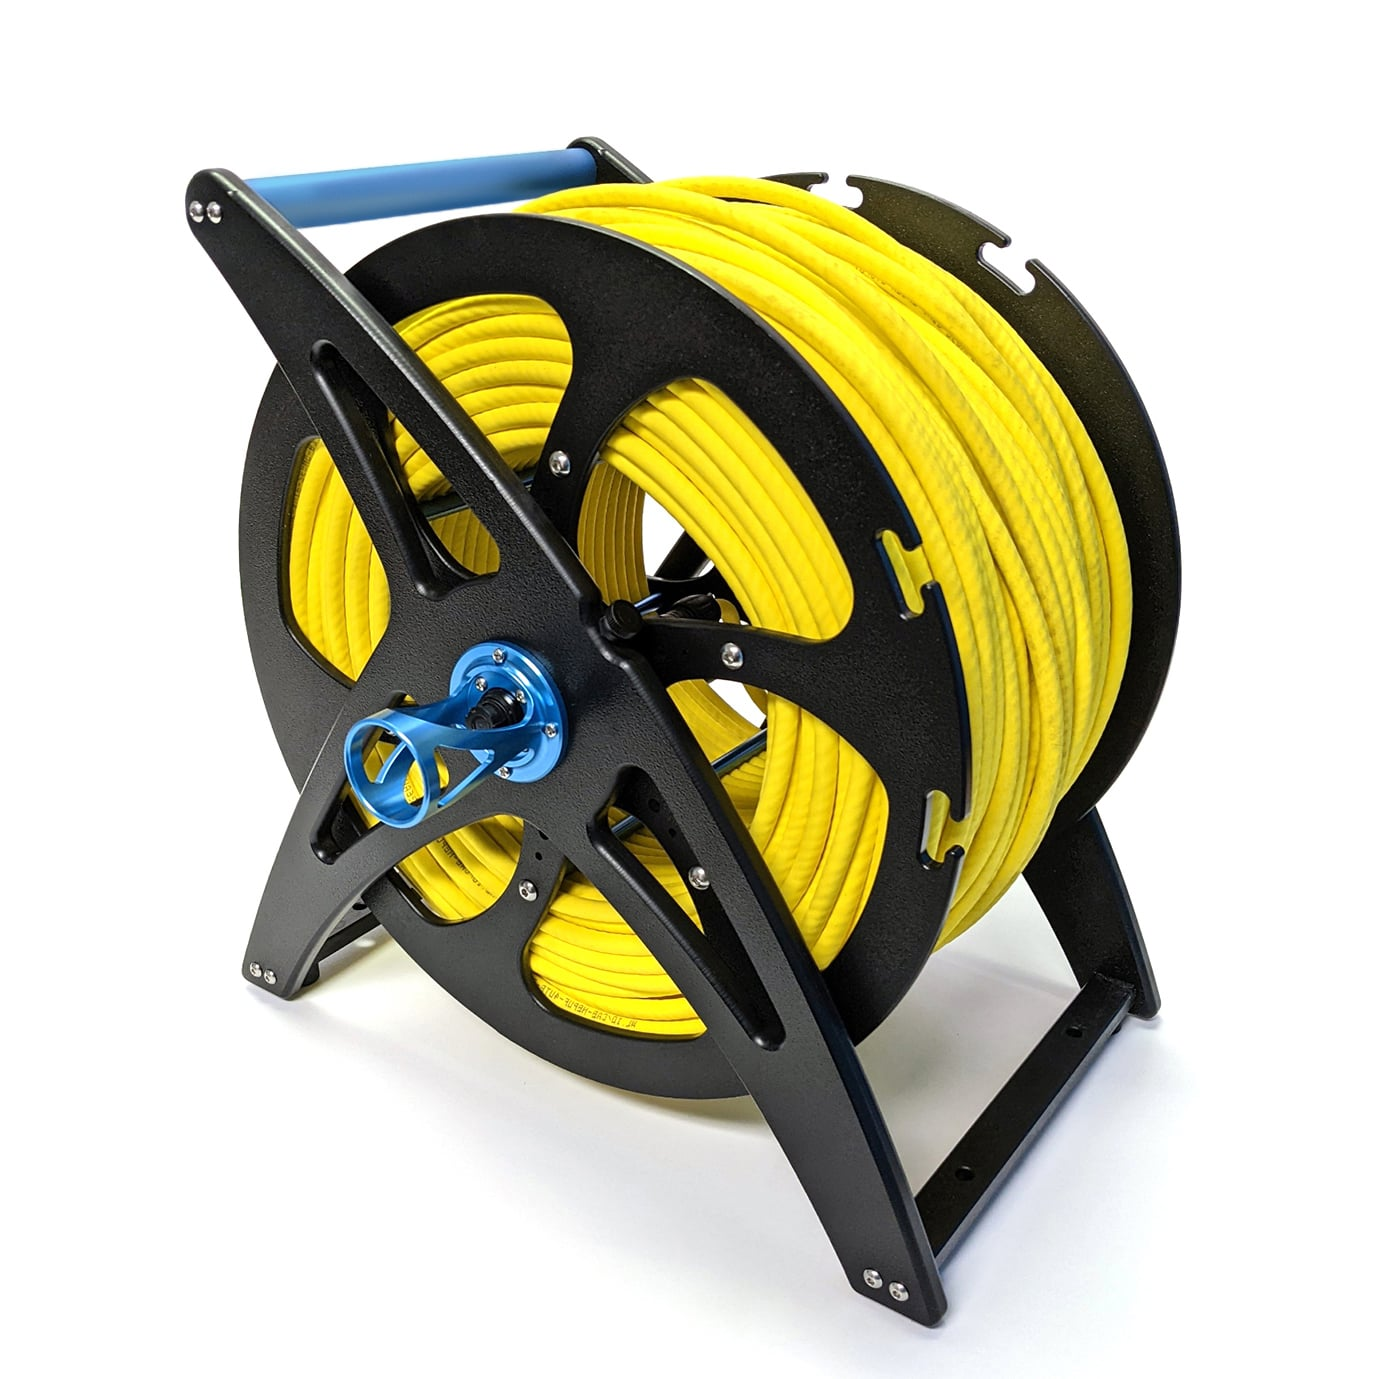
\includegraphics[height=1.4cm, keepaspectratio]{fathom_spool.jpg}\\
        \vspace{0.1em}
        \tiny\textbf{Collecteur tournant (*Slip Ring*)} \hspace{0.3cm} \textbf{Enrouleur de pont}
      \end{center}
    \end{column}
  \end{columns}
\end{frame}

\begin{frame}{3.1b Architecture des Essais : Station Sol, FXTI, BaseStation \& RC}
  \begin{columns}[c]
    \begin{column}{0.48\textwidth}
      \begin{center}
        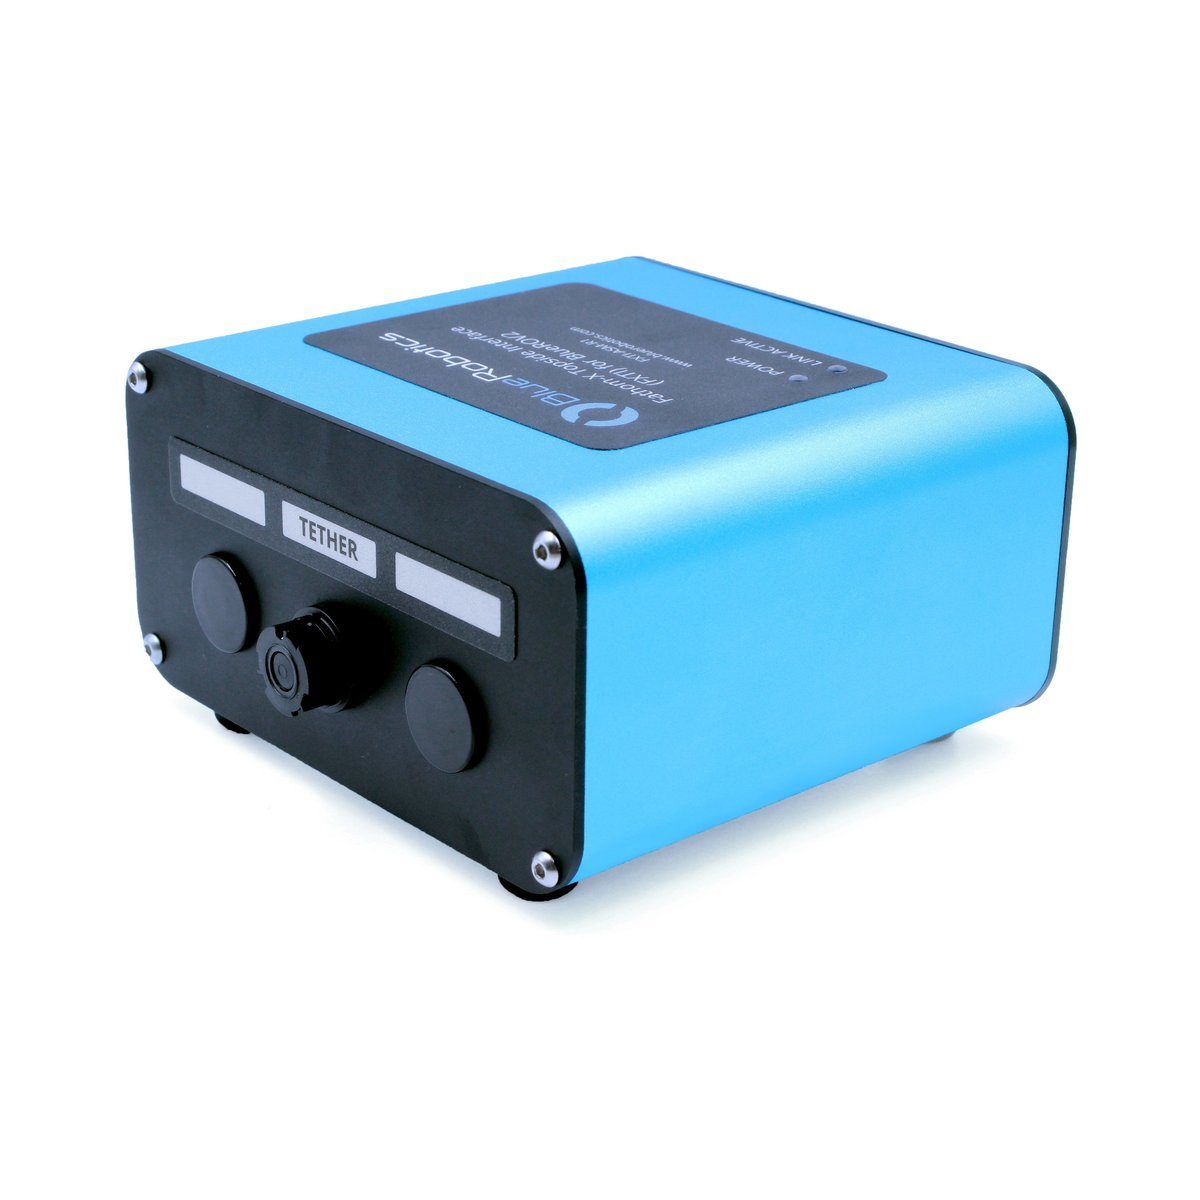
\includegraphics[height=1.5cm, keepaspectratio]{fxti_interface.jpg}
        \hspace{0.2cm}
        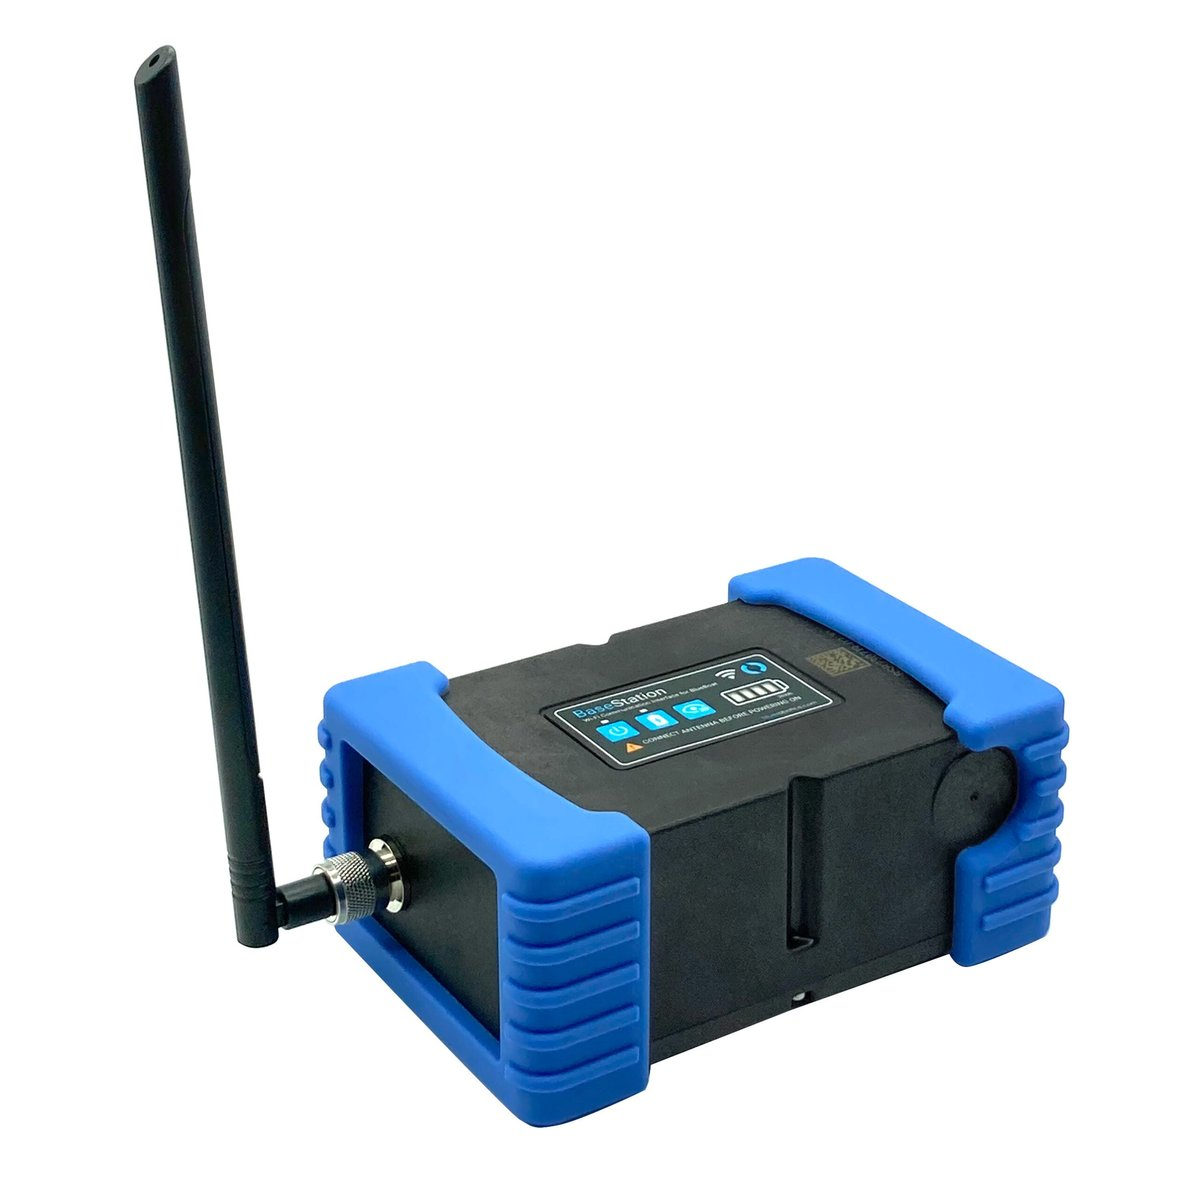
\includegraphics[height=1.5cm, keepaspectratio]{basestation_wifi.jpg}\\
        \vspace{0.1em}
        \tech{Boîtier FXTI (ROV)} \hspace{0.6cm} \succw{BaseStation WiFi (ASV)}\\
        \tiny\textit{Interface ombilical Fathom-X} \hspace{0.4cm} \textit{MikroTik 2.4 GHz longue portée}
      \end{center}
      \scriptsize
      \begin{block}{\tech{Poste de Contrôle Surface (GCS)}}
        PC durci quai/navire avec joystick USB :
        \begin{itemize}
          \item \textbf{QGroundControl} ou navigateur \textbf{Cockpit}.
          \item Visualisation télémétrie, vidéo HD, alertes.
        \end{itemize}
      \end{block}
    \end{column}

    \begin{column}{0.50\textwidth}
      \scriptsize
      \begin{block}{\tech{ROV Sous-Marin : Liaison Ombilicale}}
        \begin{itemize}
          \item Ombilical Fathom relié au boîtier \textbf{FXTI}.
          \item CPL HomePlug AV vers USB/Ethernet ($100\,\text{Mbps}$).
        \end{itemize}
      \end{block}

      \begin{block}{\succw{ASV Surface (BlueBoat) : WiFi \& Sécurité RC}}
        \begin{itemize}
          \item \textbf{BaseStation WiFi} : antenne 2.4 GHz ($>1\,\text{km}$).
          \item \alertw{Radiocommande RC manuelle (2.4 GHz SBUS)} :
            \begin{itemize}
              \item Récepteur RC direct sur le Navigator.
              \item Pilotage à vue pour mise à l'eau / quai.
              \item Sécurité matérielle immédiate (*kill-switch*).
            \end{itemize}
        \end{itemize}
      \end{block}
    \end{column}
  \end{columns}
\end{frame}

\begin{frame}{3.1c Transport d'Énergie Haute Tension : Système OTPS}
  \begin{columns}[c]
    \begin{column}{0.48\textwidth}
      \begin{center}
        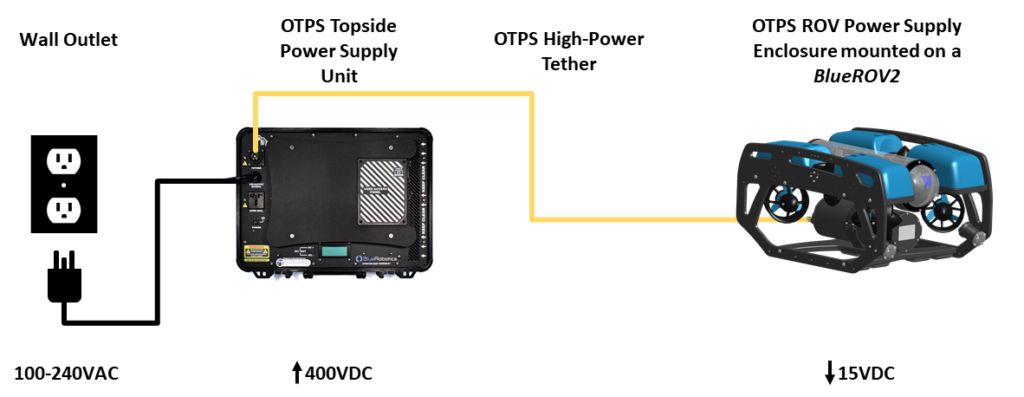
\includegraphics[width=\textwidth, height=2.8cm, keepaspectratio]{otps_power_system.png}\\
        \vspace{0.2em}
        \tech{Système OTPS (Outland Technology Power Supply)}\\
        \scriptsize\textit{Transport 400V DC par ombilical \& abaissement 15V sous-marin}
      \end{center}
      \scriptsize
      \begin{alertblock}{La Limite des Batteries}
        Autonomie limitée à $2\text{--}4\,\text{h}$. Remplacement de batterie fastidieux obligeant à sortir et sécher le robot.
      \end{alertblock}
    \end{column}

    \begin{column}{0.50\textwidth}
      \textbf{La physique du transport haute tension} :
      \scriptsize
      \begin{itemize}
        \item Puissance transportée : $P = U \cdot I$.
        \item Pour transmettre $1000\,\text{W}$ sur $300\,\text{m}$ :
          \begin{itemize}
            \item En basse tension ($15\,\text{V}$) : $I \approx 67\,\text{A}$ $\rightarrow$ pertes Joule destructrices ($P = R I^2$).
            \item En haute tension (\succw{$400\,\text{V DC}$}) : $I \approx 2.5\,\text{A}$ !
          \end{itemize}
        \item Pertes Joule divisées par $(400/15)^2 \approx \succw{700}$ !
      \end{itemize}

      \vspace{0.2em}
      \begin{block}{\succw{Architecture Électronique Embarquée}}
        \begin{itemize}
          \item \textbf{Boîtier Surface} : redresse le secteur $110/240\,\text{V AC}$ vers $400\,\text{V DC}$ régulé.
          \item \textbf{Carte de Puissance Sous-Marine} : hacheur abaisseur DC-DC isolé dans le caisson du ROV, convertissant le $400\,\text{V DC}$ en \textbf{$15\,\text{V DC}$ continu (jusqu'à $45\,\text{A}$ / $1000\,\text{W}$)}.
          \item Permet des plongées illimitées (24h/24) !
        \end{itemize}
      \end{block}
    \end{column}
  \end{columns}
\end{frame}

\begin{frame}{3.2 Le C{\oe}ur Logiciel Moderne : L'Écosystème BlueOS}
  \begin{columns}[T]
    \begin{column}{0.5\textwidth}
      \begin{block}{\tech{Qu'est-ce que BlueOS ?}}
        \begin{itemize}
          \item Le système d'exploitation embarqué moderne de BlueRobotics (remplaçant historique du script Python \textit{companion}).
          \item Tourne sur le \textbf{Raspberry Pi 4 / 5} (base Linux Debian).
          \item Architecture entièrement conteneurisée via \textbf{Docker} :
            \begin{itemize}
              \item Service vidéo WebRTC / RTSP ultra-faible latence.
              \item Routeur MAVLink centralisé (MAVLink2Rest).
              \item Flasheur de firmware d'autopilote en un clic.
            \end{itemize}
        \end{itemize}
      \end{block}
    \end{column}

    \begin{column}{0.5\textwidth}
      \begin{block}{\succw{Avantages Clés pour le Scientifique}}
        \begin{itemize}
          \item \textbf{Zéro logiciel à installer en surface} : accessible depuis un simple navigateur web sur \code{http://blueos.local} ou \code{192.168.2.2}.
          \item Gestionnaire de fichiers web pour télécharger les logs directement.
          \item Terminal SSH interactif intégré dans l'interface web.
          \item Monitoring complet : température CPU, tension d'alimentation, usage mémoire.
        \end{itemize}
      \end{block}
    \end{column}
  \end{columns}
\end{frame}

\begin{frame}{3.3 Le Magasin d'Extensions BlueOS pour la Recherche}
  \begin{columns}[c]
    \begin{column}{0.55\textwidth}
      \textbf{Comment intégrer vos propres capteurs ?}
      \begin{itemize}
        \item BlueOS dispose d'un gestionnaire d'\textbf{Extensions conteneurisées} (similaire à un "App Store" de bord).
        \item N'importe quel chercheur ou ingénieur peut créer son conteneur Docker avec un script Python de lecture de capteur (sonde CTD, fluorimètre, sonar).
        \item L'extension peut exposer :
          \begin{itemize}
            \item Une page web dédiée dans BlueOS.
            \item Des flux de données MAVLink personnalisés.
            \item Un broker de données partagé.
          \end{itemize}
        \item Installation et mise à jour en 1 clic sans risque de corrompre le système de base du drone.
      \end{itemize}
    \end{column}

    \begin{column}{0.45\textwidth}
      \begin{block}{Extensions Déjà Disponibles}
        \begin{itemize}
          \item \tech{Ping Viewer} : visualisation sonar Ping / Ping360.
          \item \tech{DVL Extension} : driver et interface Water Linked DVL-A50.
          \item \tech{NMEA Injector} : injection de GPS de surface vers l'autopilote.
          \item \tech{Node-RED} : automatisation de flux de données sans coder.
          \item \tech{ROS 2 Bridge} : communication native avec l'écosystème robotique.
        \end{itemize}
      \end{block}
    \end{column}
  \end{columns}
\end{frame}

\begin{frame}{3.4 Interfaces de Contrôle : QGroundControl vs Cockpit}
  \begin{columns}[T]
    \begin{column}{0.48\textwidth}
      \begin{center}
        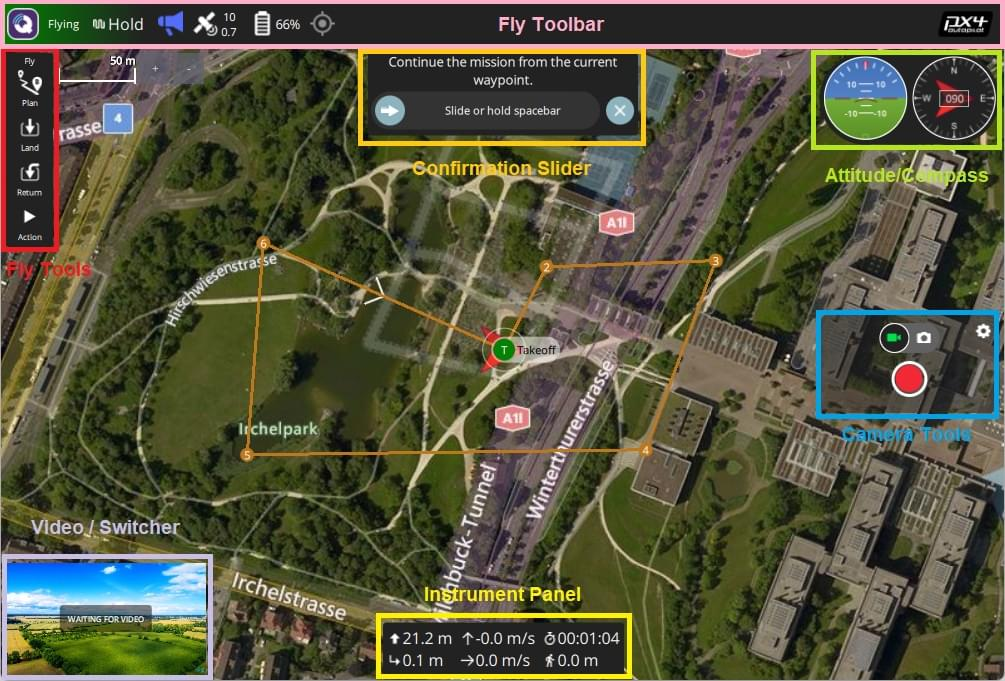
\includegraphics[width=\linewidth, height=2.45cm, keepaspectratio]{qgroundcontrol_interface.jpg}\\
        \vspace{0.15em}
        \tech{QGroundControl (QGC)}\\
        \tiny\textit{Station sol native (C++ / Qt) --- Vue Télémétrie \& HUD}
      \end{center}
      \vspace{-0.4em}
      \begin{block}{QGroundControl : Le Standard Éprouvé}
        \scriptsize
        \begin{itemize}
          \item \textbf{Application native historique} (15 ans) : multiplateforme (PC, Mac, Linux, tablettes).
          \item \textbf{Fonctions} : calibrage joysticks/capteurs, incrustation vidéo HUD, planification de waypoints.
          \item \alertw{Limite} : rigide, difficile d'intégrer des widgets pour sondes océanographiques sur-mesure.
        \end{itemize}
      \end{block}
    \end{column}

    \begin{column}{0.48\textwidth}
      \begin{center}
        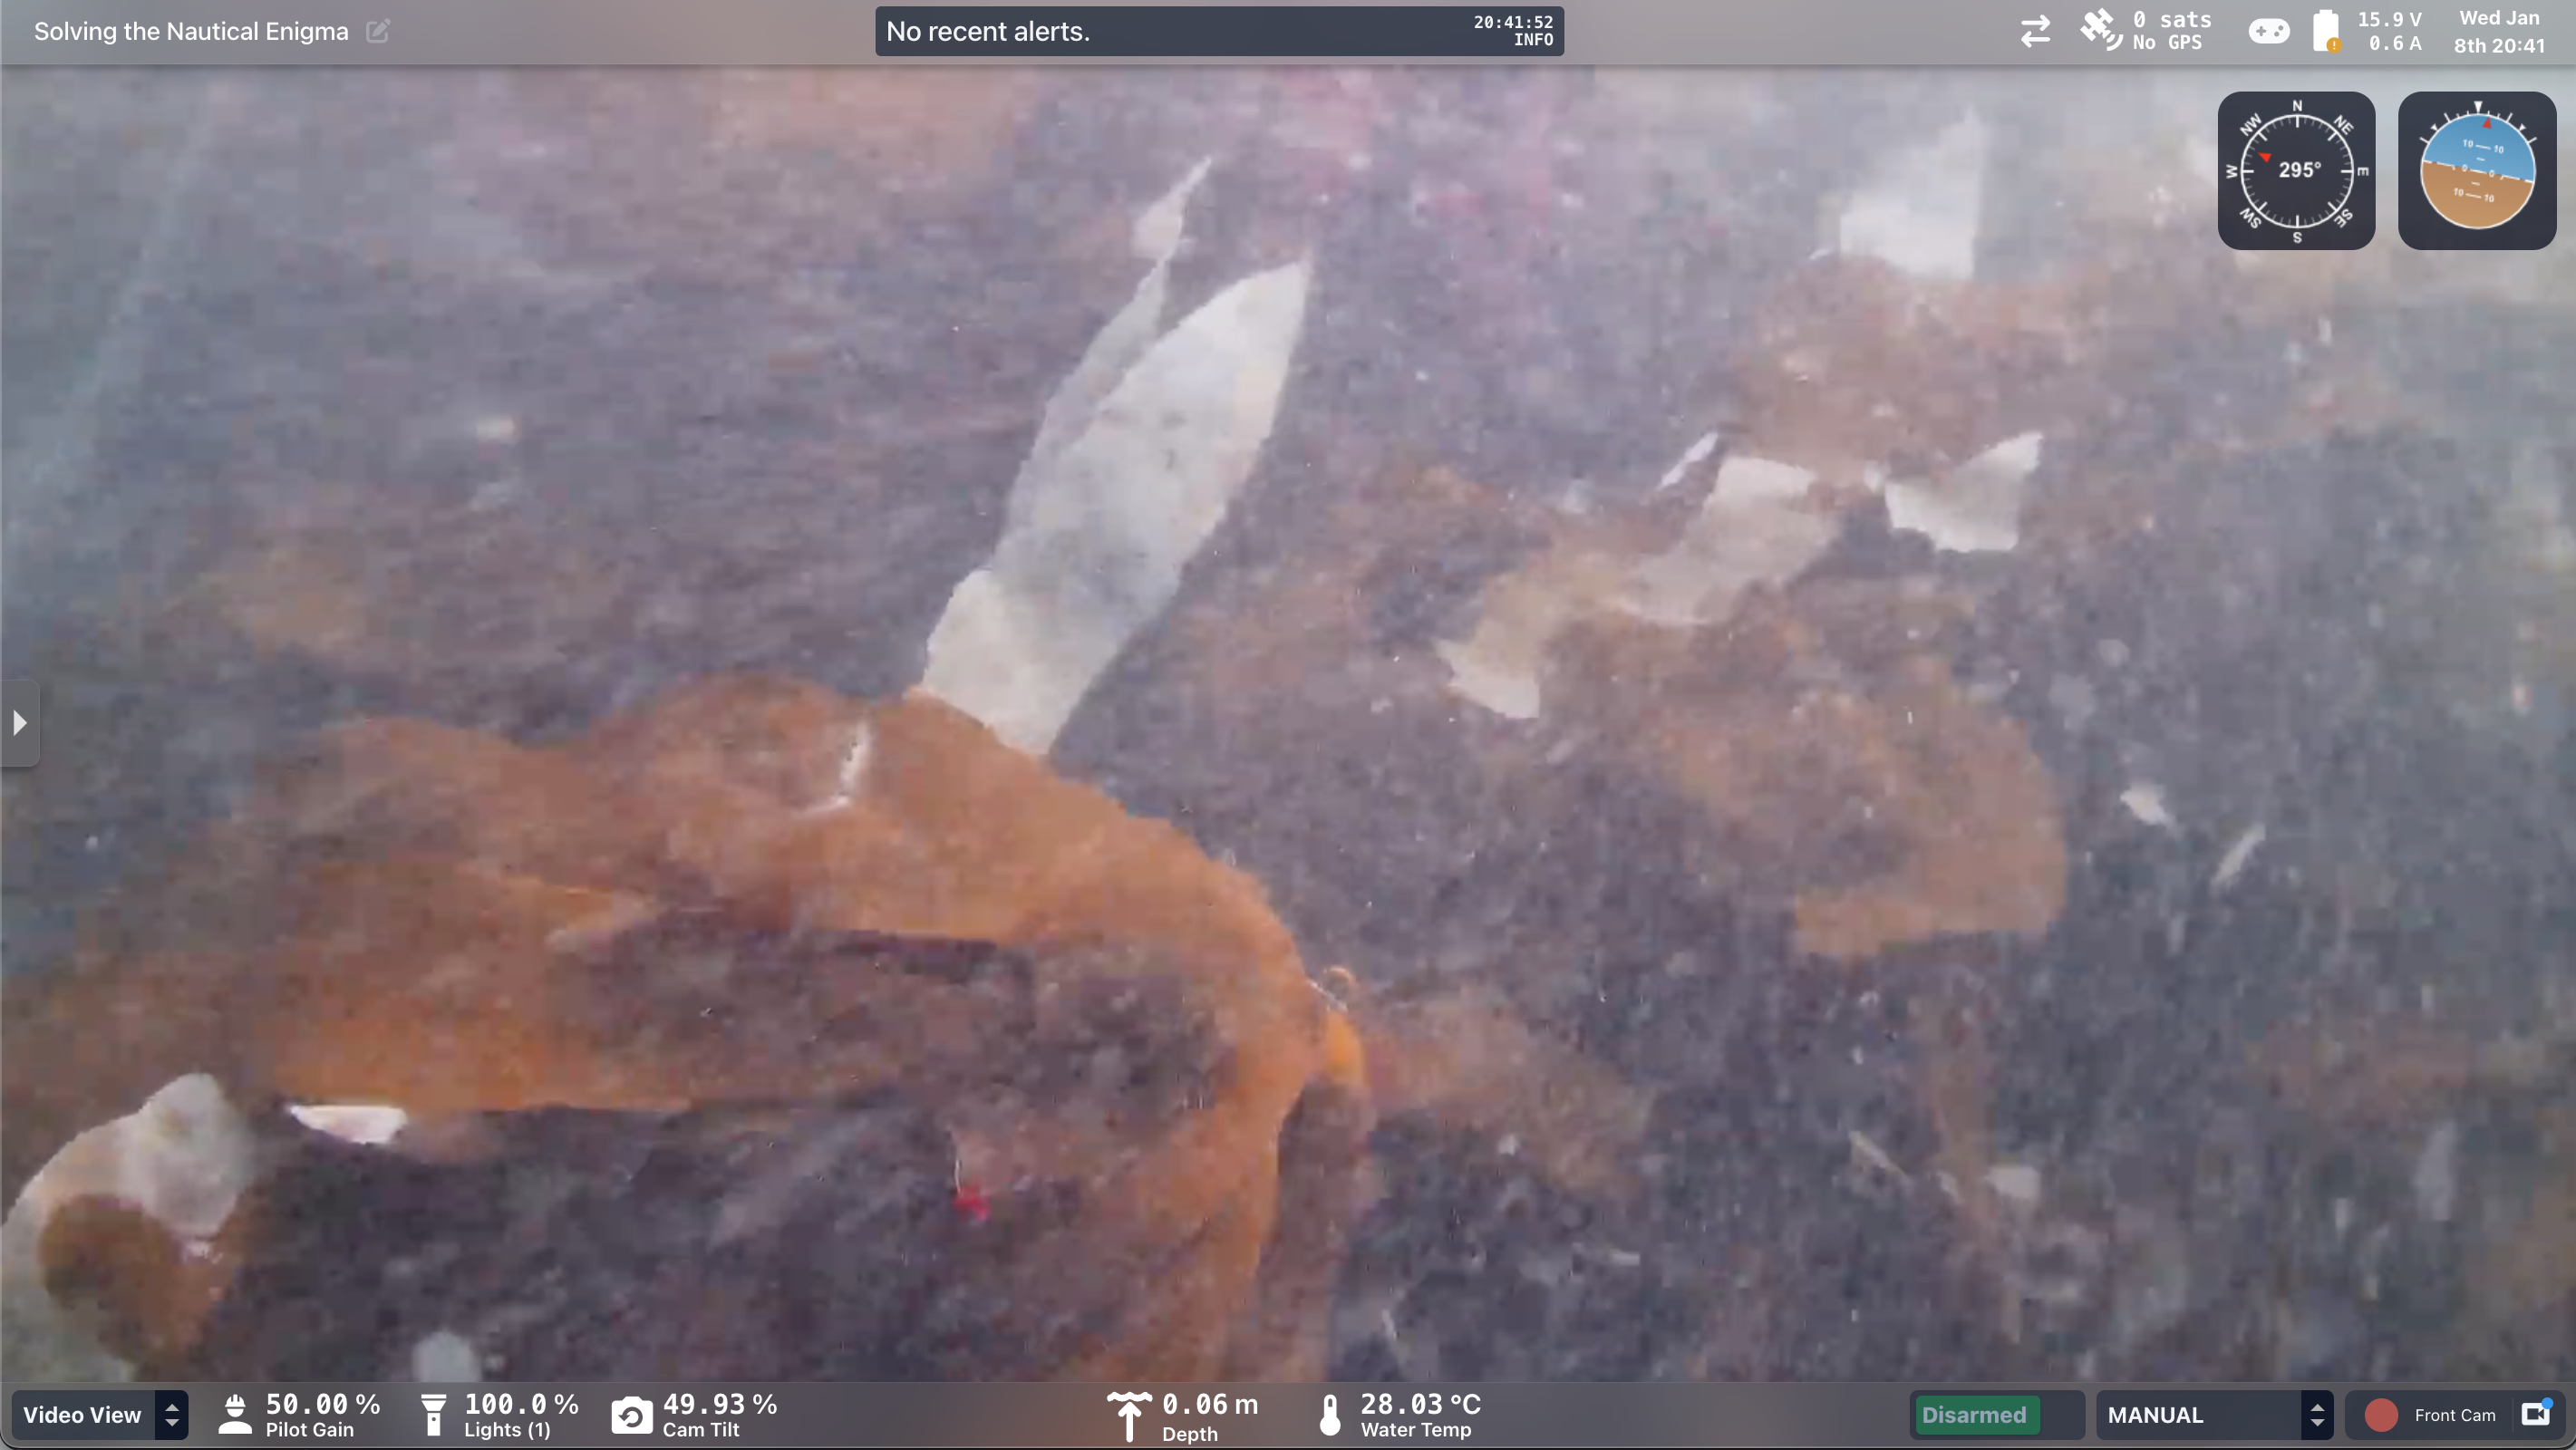
\includegraphics[width=\linewidth, height=2.45cm, keepaspectratio]{sub-video-view.png}\\
        \vspace{0.15em}
        \succw{Cockpit (BlueRobotics)}\\
        \tiny\textit{Interface web moderne (HTML5 / Vue.js) --- Vue Vidéo ROV}
      \end{center}
      \vspace{-0.4em}
      \begin{block}{Cockpit : La Nouvelle Génération Web}
        \scriptsize
        \begin{itemize}
          \item \textbf{Zéro installation client} : tourne directement dans le navigateur (Chrome / Firefox) via BlueOS.
          \item \textbf{100\% modulaire} : organisation des vues et panneaux en glisser-déposer (\textit{drag \& drop}).
          \item \succw{Personnalisable} : développement facile de widgets scientifiques (sonde CTD, sonar, etc.).
        \end{itemize}
      \end{block}
    \end{column}
  \end{columns}
\end{frame}

\begin{frame}{3.4b Cockpit en Pratique : Vues Métier Dédiées (ROV vs ASV)}
  \begin{columns}[T]
    \begin{column}{0.48\textwidth}
      \begin{center}
        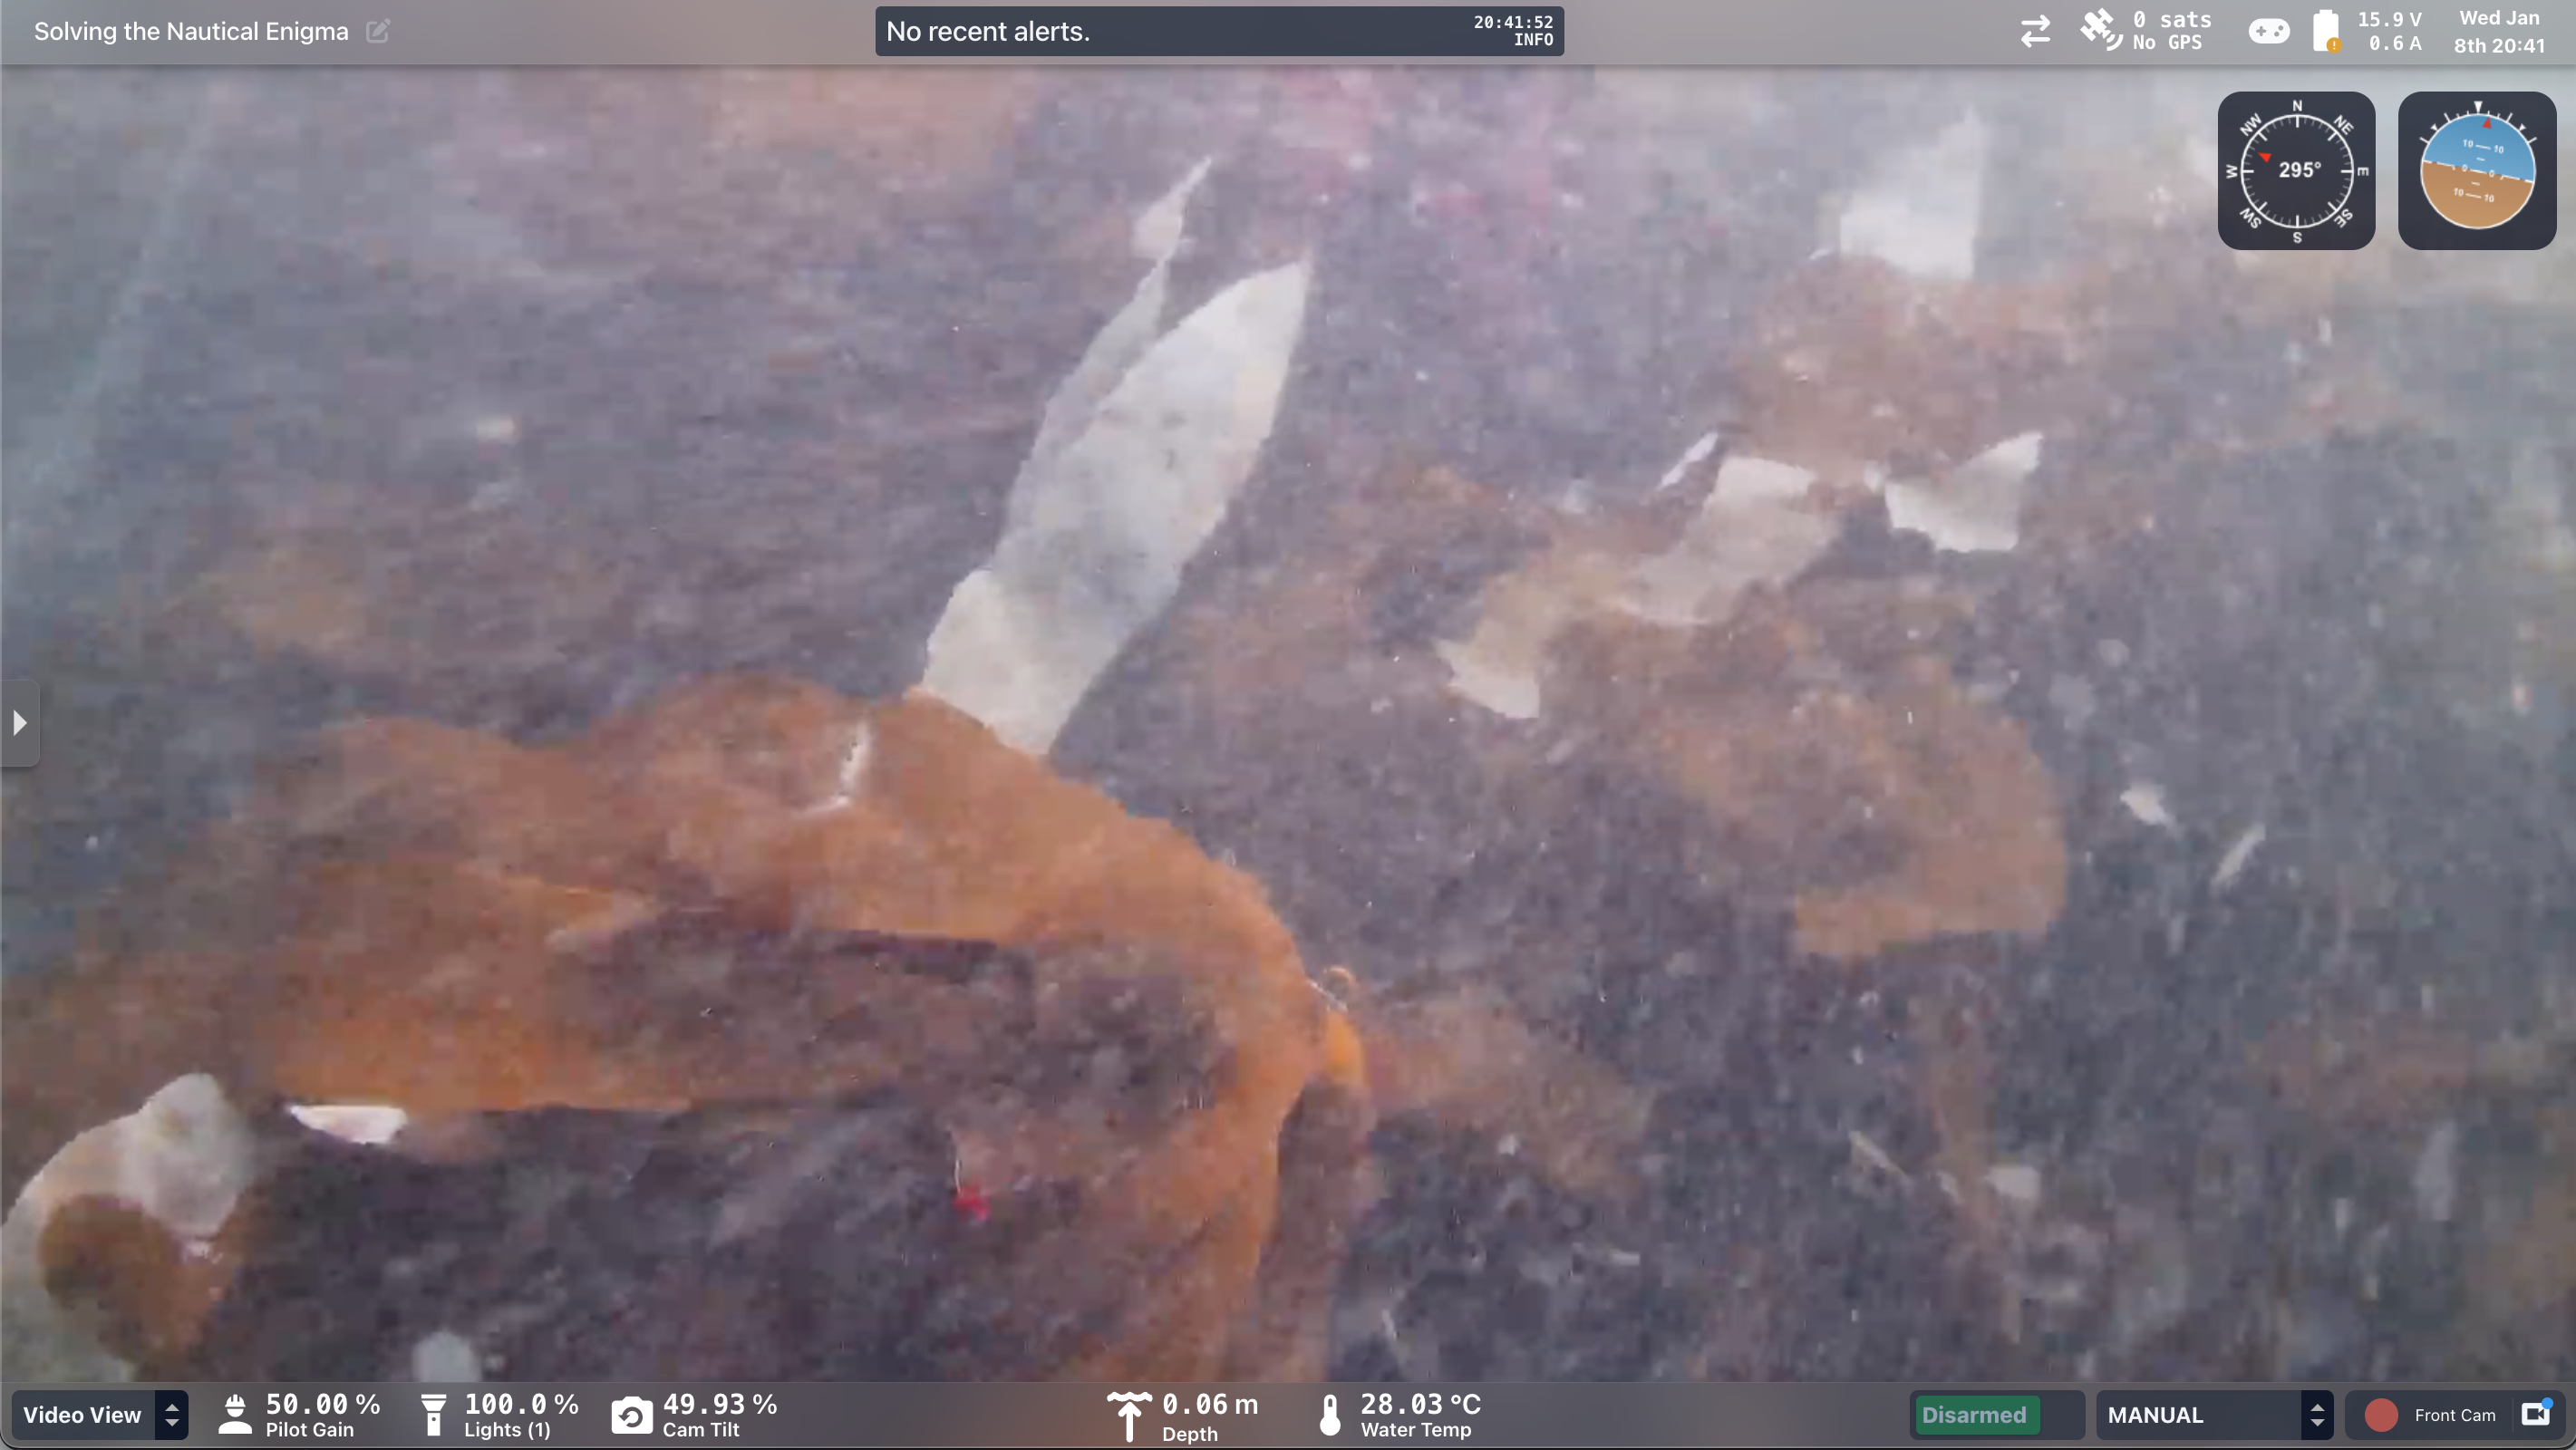
\includegraphics[width=\linewidth, height=2.35cm, keepaspectratio]{sub-video-view.png}\\
        \vspace{0.15em}
        \tech{Vue Vidéo \& Pilotage ROV (BlueROV2)}\\
        \tiny\textit{Inspection subaquatique, capteurs de sûreté et commandes directes}
      \end{center}
      \vspace{-0.4em}
      \begin{block}{Pilotage Subaquatique Immergé}
        \scriptsize
        \begin{itemize}
          \item \textbf{Flux vidéo temps réel} : caméra grand angle, contrôle de tilt ($\pm 90^\circ$) et variateur des projecteurs Lumen.
          \item \textbf{Incrustation vitale} : profondeur Bar30, cap, température de l'eau, assiette et tension/courant batterie.
          \item \textbf{Modes de vol} : bascule directe Manuel / Stabilize / Depth Hold.
        \end{itemize}
      \end{block}
    \end{column}

    \begin{column}{0.48\textwidth}
      \begin{center}
        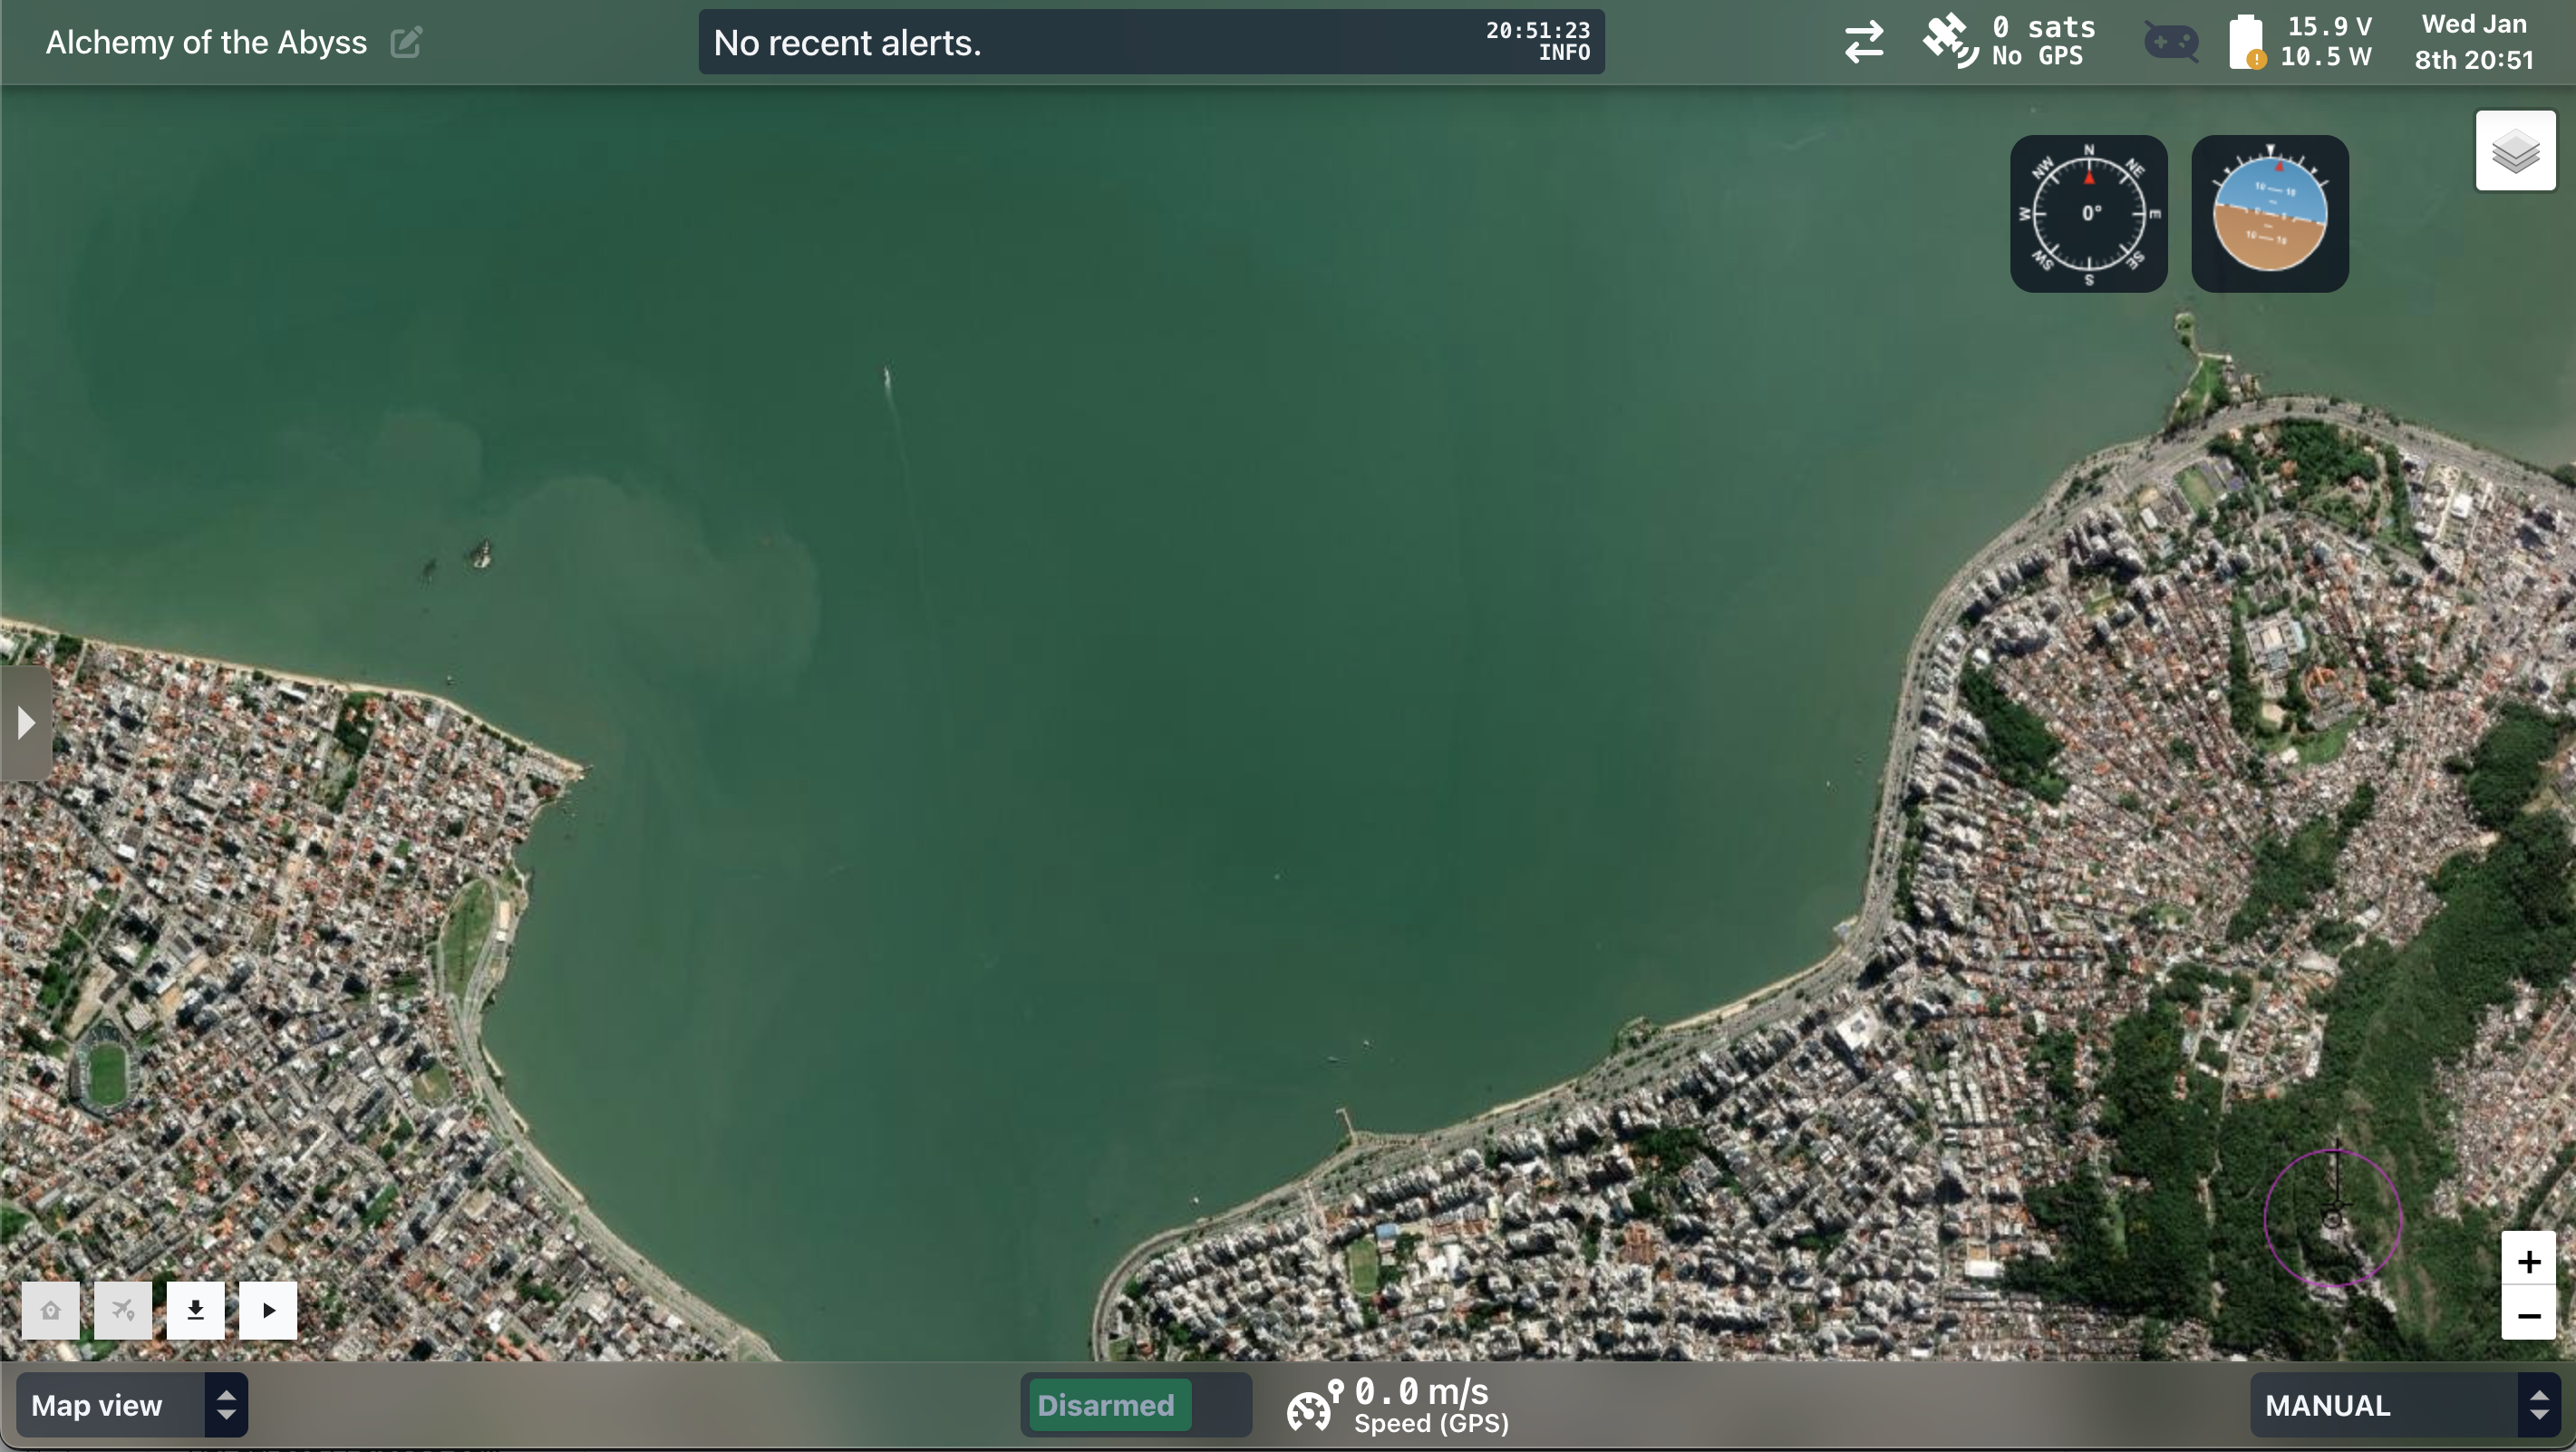
\includegraphics[width=\linewidth, height=2.35cm, keepaspectratio]{boat-map-view.png}\\
        \vspace{0.15em}
        \succw{Vue Cartographique ASV (BlueBoat)}\\
        \tiny\textit{Suivi de mission, géoréférencement GNSS RTK et bathymétrie}
      \end{center}
      \vspace{-0.4em}
      \begin{block}{Navigation \& Relevé Surfacique}
        \scriptsize
        \begin{itemize}
          \item \textbf{Fond de carte satellite} : centrage automatique sur la trace GPS haute précision du navire.
          \item \textbf{Planification autonome} : tracé de transects réguliers pour fauchée acoustique ou profils CTD.
          \item \textbf{Surveillance distante} : vitesse sol, satellites GNSS, télémétrie sol WiFi ($>500\,\text{m}$).
        \end{itemize}
      \end{block}
    \end{column}
  \end{columns}
\end{frame}
\begin{frame}{3.5 L'Intégration ROS / ROS 2 pour les Data Scientists}
  \begin{center}
    \begin{tikzpicture}[scale=0.85, auto, node distance=1.2cm, >=Latex]
      \node[draw=OceanMedium, fill=OceanMedium!15, rounded corners, rectangle, minimum width=2.6cm, align=center] (ardusub) {
        \textbf{ArduSub / Rover}\\
        \footnotesize MAVLink Stream
      };
      \node[draw=OceanDeep, fill=OceanDeep!20, rounded corners, rectangle, minimum width=2.8cm, align=center, right=1.2cm of ardusub] (mavros) {
        \textbf{Pont ROS 2}\\
        \footnotesize \code{mavros} ou micro-ROS
      };
      \node[draw=OceanGreen, fill=OceanGreen!15, rounded corners, rectangle, minimum width=3.4cm, align=center, right=1.2cm of mavros] (rostopics) {
        \textbf{Topics ROS 2}\\
        \footnotesize \code{/mavros/imu/data}\\
        \footnotesize \code{/mavros/local\_position}\\
        \footnotesize \code{/sensor/ocean\_ctd}
      };
      \node[draw=OceanCyan, fill=OceanCyan!20, line width=1.2pt, rounded corners, rectangle, minimum width=3.4cm, align=center, below=0.8cm of rostopics] (rosbag) {
        \textbf{Enregistrement ROSBAG2}\\
        \footnotesize Fichiers \textbf{.mcap} complets\\
        \footnotesize Horodatage nanoseconde
      };

      \draw[->, thick, OceanDeep] (ardusub) -- (mavros);
      \draw[->, thick, OceanDeep] (mavros) -- (rostopics);
      \draw[->, line width=1.5pt, OceanCyan] (rostopics) -- (rosbag);
    \end{tikzpicture}
  \end{center}

  \begin{block}{Pourquoi ROS 2 est l'outil ultime pour le traitement de données ?}
    \begin{itemize}
      \item \textbf{Synchronisation de messages (\code{message\_filters})} : fusionne automatiquement la navigation (DVL/IMU) et les mesures scientifiques au même instant $t$.
      \item \textbf{Gestion des repères spatiaux (\code{tf2})} : gère le bras de levier (*lever arm*) entre le centre de gravité, le DVL, la caméra et le capteur CTD.
    \end{itemize}
  \end{block}
\end{frame}

\begin{frame}{3.5b Logs Telemetry Dataflash (.bin), Rejeu \& UAV Log Viewer}
  \begin{columns}[T]
    \begin{column}{0.48\textwidth}
      \begin{block}{\tech{Les Logs Bruts Autopilote (.bin)}}
        \scriptsize
        \begin{itemize}
          \item ArduSub enregistre en continu des fichiers de télémétrie binaire Dataflash \code{.bin} directement sur la carte SD ou la mémoire Flash du calculateur (RPi/Navigator/Pixhawk).
          \item Contiennent \textbf{toutes les données internes à 50 Hz--400 Hz} : attitudes IMU, consignes moteurs PWM, profondeurs Bar30, états des fail-safes et pings DVL.
          \item Indispensables pour l'expertise post-incident et la reconstruction exacte de la plongée.
        \end{itemize}
      \end{block}

      \begin{block}{\succw{Rejeu \& Traitement Hors-Ligne}}
        \scriptsize
        \begin{itemize}
          \item \textbf{Rejeu MAVLink (QGC)} : rejouer la mission entière seconde par seconde comme en direct sur le terrain.
          \item \textbf{Pipeline Python (\code{pymavlink})} : export direct vers \code{pandas} / CSV pour traitement scientifique.
        \end{itemize}
      \end{block}
    \end{column}

    \begin{column}{0.48\textwidth}
      \begin{center}
        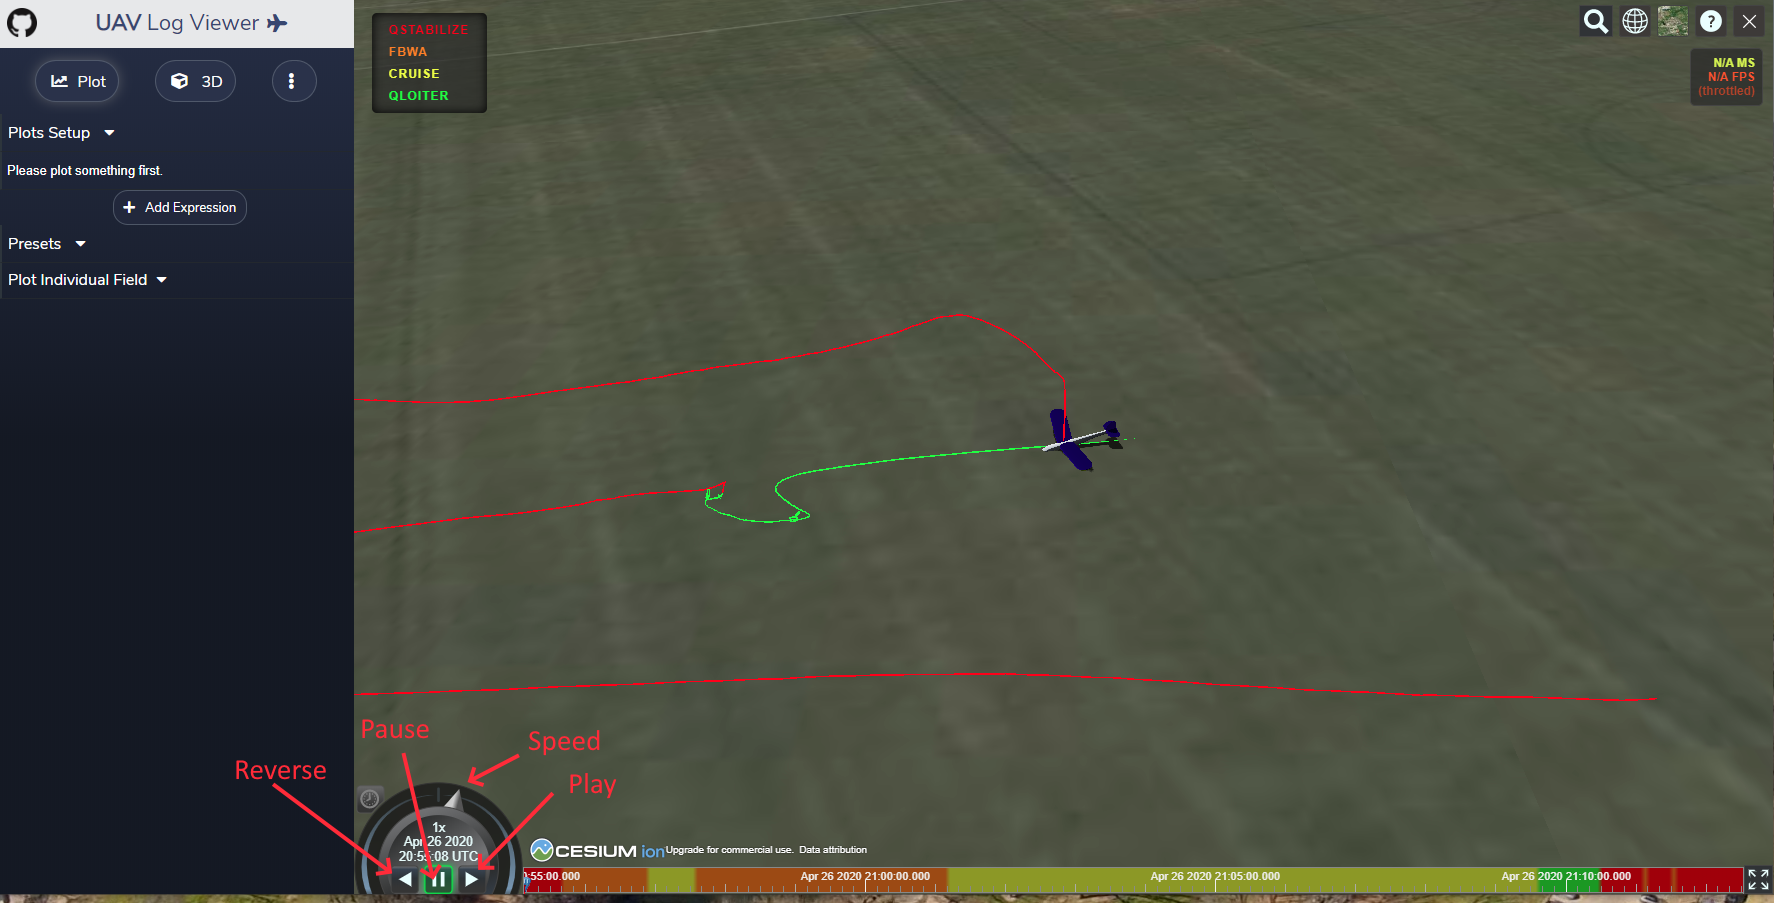
\includegraphics[width=\linewidth, height=2.6cm, keepaspectratio]{uav_logviewer.png}\\
        \vspace{0.15em}
        \succw{UAV Log Viewer (\href{https://plot.ardupilot.org}{\code{plot.ardupilot.org}})}\\
        \tiny\textit{Visualisation 3D, spectres de vibrations IMU \& analyse temporelle}
      \end{center}
      \vspace{-0.4em}
      \begin{block}{Diagnostic Visuel \& Rejeu en Ligne}
        \scriptsize
        \begin{itemize}
          \item \textbf{Zéro installation} : glisser-déposer direct du fichier \code{.bin} dans le navigateur web.
          \item \textbf{Trajectoire 3D dynamique} : suivi spatial synchronisé avec les graphes de capteurs (batterie, cap, profondeur).
          \item \textbf{Analyse fréquentielle (FFT)} : détection des résonances mécaniques et vibrations propulseurs.
        \end{itemize}
      \end{block}
    \end{column}
  \end{columns}
\end{frame}

\begin{frame}{3.6 Capteurs de Sûreté Véhicule \& Fail-Safes Réels}
  \begin{table}[h]
    \centering
    \scriptsize
    \begin{tabularx}{\textwidth}{l p{4.2cm} X}
      \toprule
      \textbf{Capteur de Sûreté} & \textbf{Principe \& Implantation} & \textbf{Réaction Automatique (Fail-Safe)} \\
      \midrule
      \alertw{SOS Leak Sensor} & Bandes conductimétriques au point le plus bas des caissons (électronique \& batterie) & Alerte sonore QGC/Cockpit, clignotement des feux Lumen, désarmement propulsion, remontée passive \\
      \alertw{Pression interne} & Surveillance de la dépression post-test de vide ($<-0.4\,\text{bar}$) & Détection d'infiltration d'air/eau \succw{avant tout contact liquide avec l'électronique} \\
      \alertw{Sonde Power Sense} & Mesure courant crête ($<60\,\text{A}$) et tension cellule Li-ion ($>3.3\,\text{V}$) & Alerte tension basse, coupure préventive des charges utiles secondaires \\
      \alertw{Heartbeat MAVLink} & Perte de communication ombilical ou WiFi ($>5\,\text{s}$) & Mode \textbf{Disarm} automatique, coupure moteurs et retour de surface par flottabilité positive \\
      \bottomrule
    \end{tabularx}
  \end{table}

  \begin{block}{\tech{Philosophie des Fail-Safes Réseau \& Matériels}}
    \scriptsize
    Chaque capteur de sûreté est relié à une boucle d'asservissement matérielle ou logicielle sous ArduSub/BlueOS. En cas de défaillance critique, le robot privilégie toujours sa \succw{remontée passive en surface} et la préservation de ses données embarquées.
  \end{block}
\end{frame}

\begin{frame}{3.6b Focus Matériel : Le SOS Leak Sensor}
  \begin{columns}[c]
    \begin{column}{0.40\textwidth}
      \begin{center}
        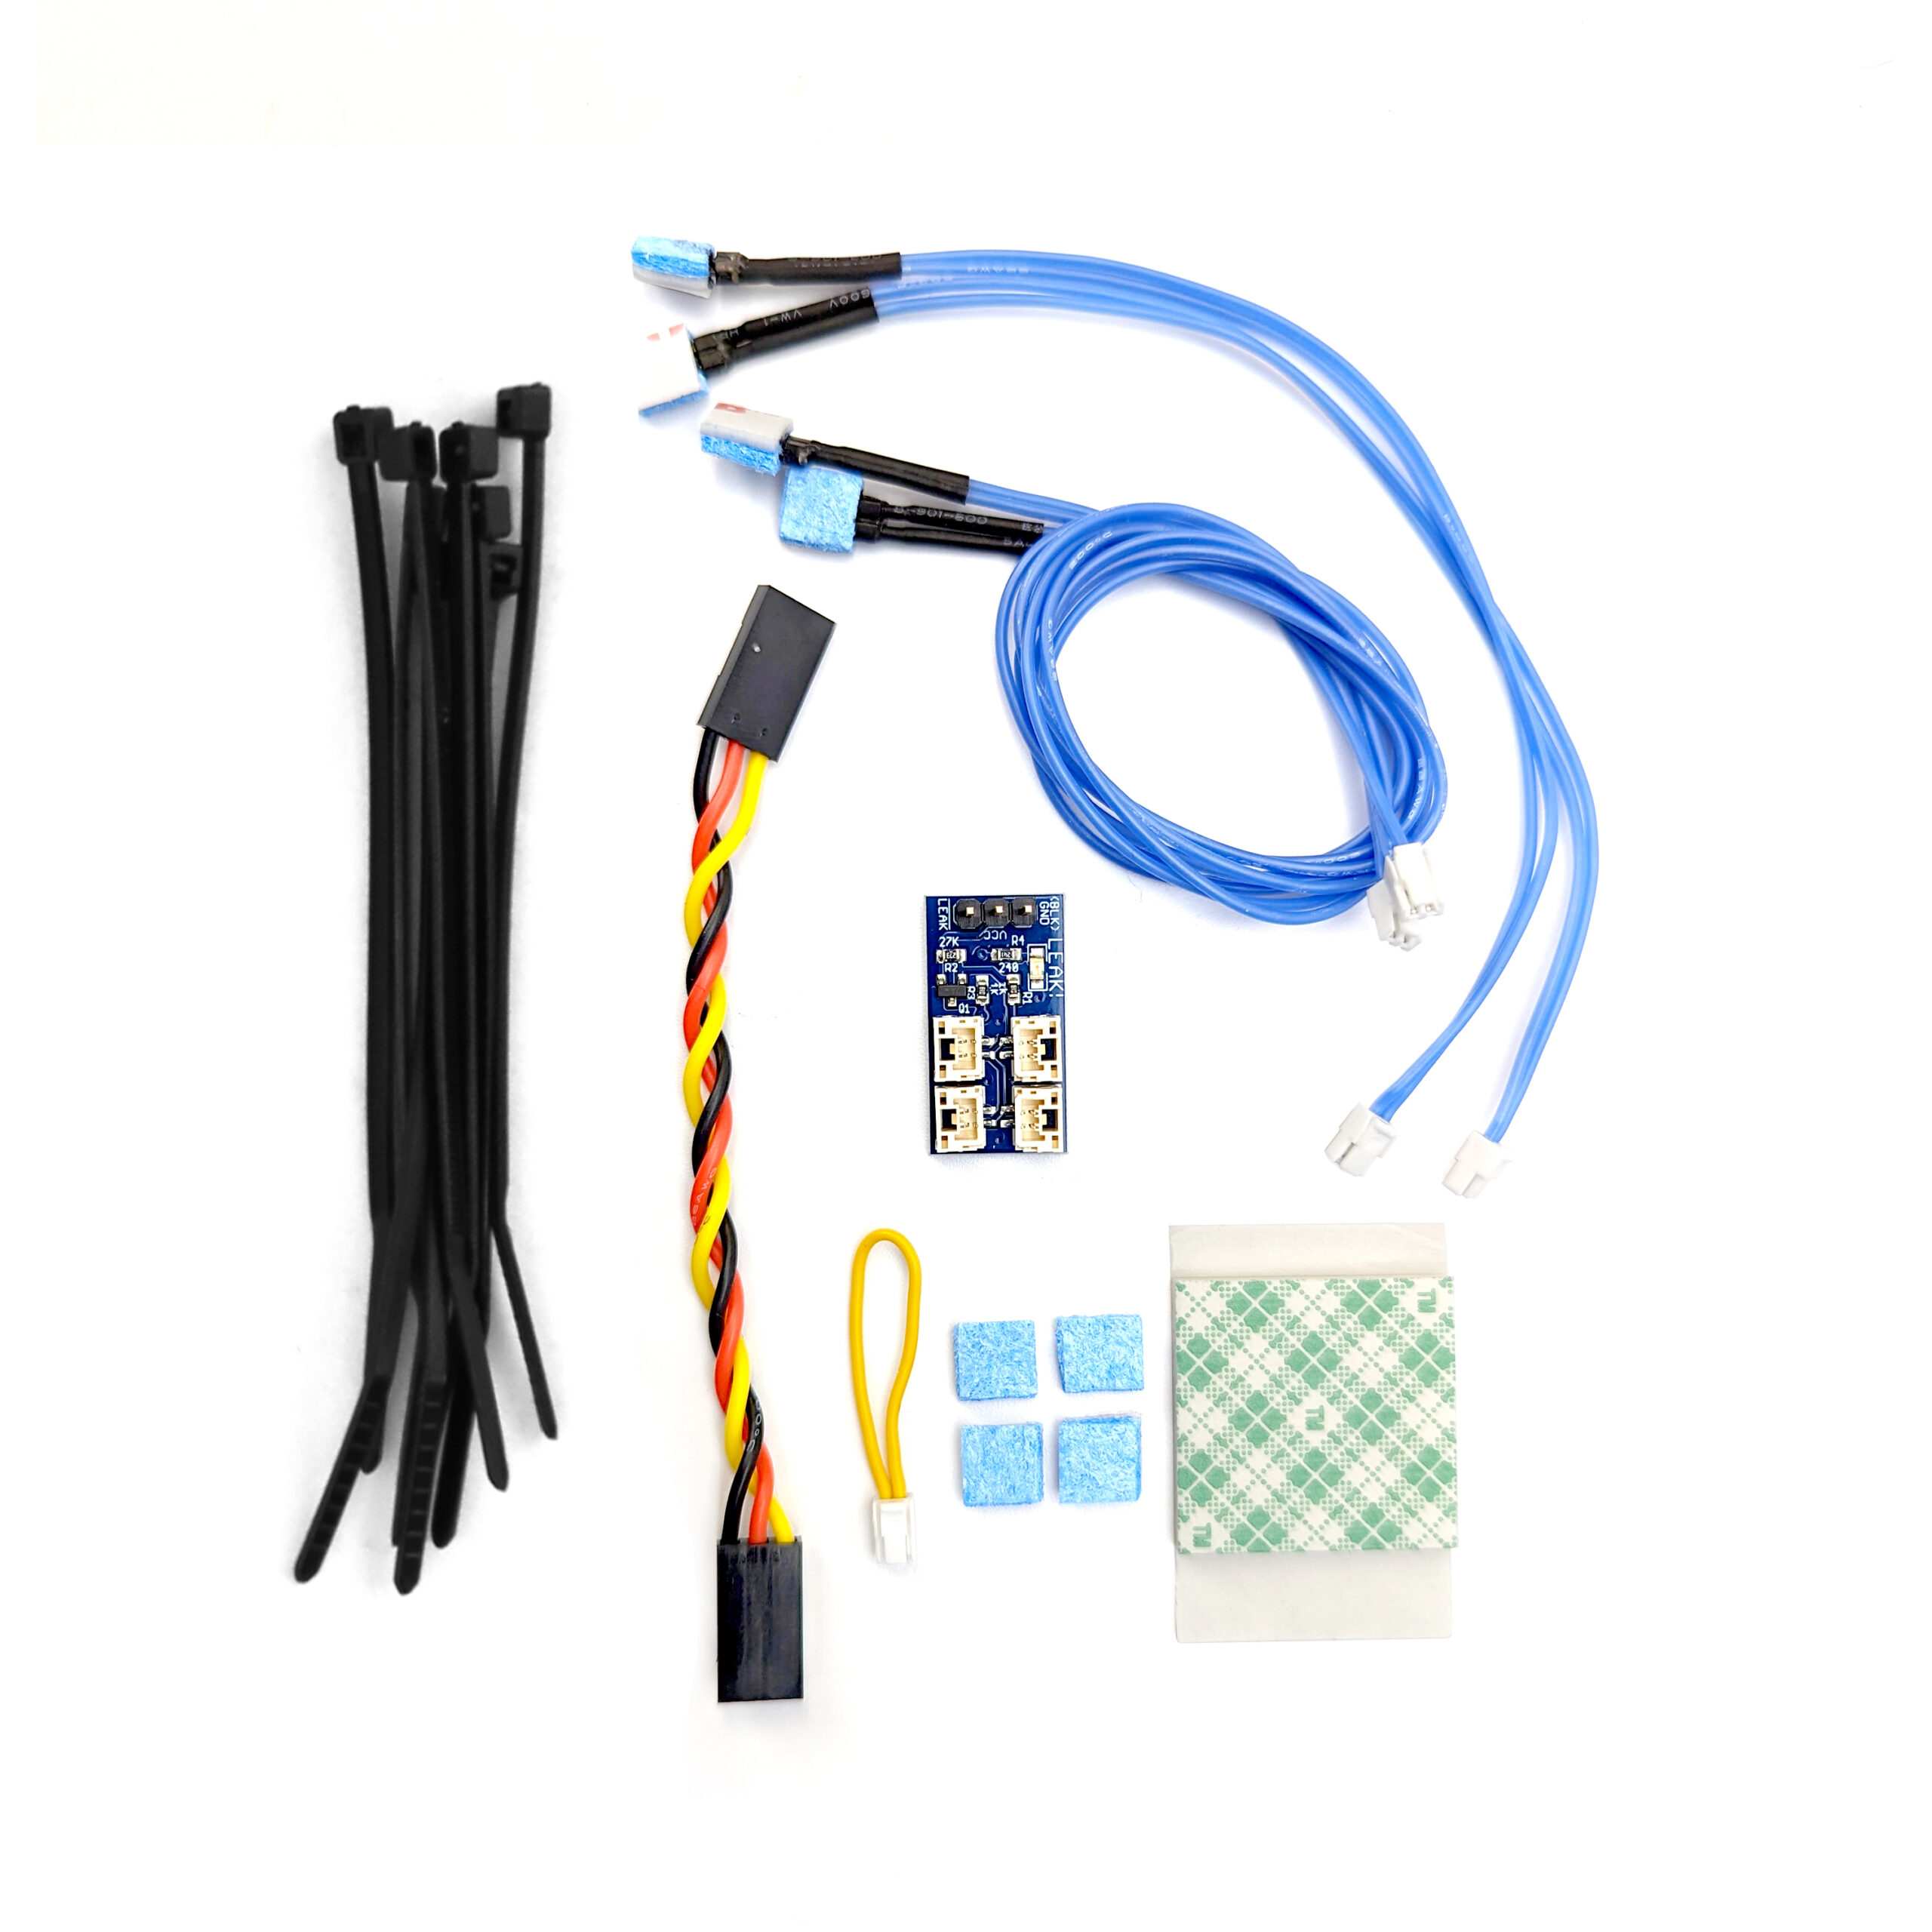
\includegraphics[height=3.4cm, keepaspectratio]{sos_leak_sensor.jpg}\\
        \vspace{0.2em}
        \footnotesize\textbf{BlueRobotics SOS Leak Sensor}\\
        \scriptsize\textit{Circuit comparateur \& sondes conductives}
      \end{center}
    \end{column}

    \begin{column}{0.58\textwidth}
      \begin{block}{\tech{Fonctionnement du SOS Leak Sensor}}
        \scriptsize
        \begin{itemize}
          \item Circuit comparateur connecté directement sur une entrée GPIO de l'autopilote (carte Navigator / Pixhawk).
          \item Rubans adhésifs à pistes interdigitées tapissant le fond du tube : la moindre goutte salée ou douce ferme le circuit par conduction.
          \item Déclenche l'alerte sonore Cockpit/QGC et le clignotement d'urgence des feux Lumen.
        \end{itemize}
      \end{block}
    \end{column}
  \end{columns}
\end{frame}

% ==============================================================================
% 04_capteurs_donnees.tex - Module 4 (15h30 - 16h30)
% Exemple de capteurs et mesures spécifiques : de la collecte à la donnée
% Pratique : Ping Sonar, Ping360, DVL-A50, intégration d'une sonde scientifique tierce
% ==============================================================================

\section{Module 4 : Capteurs Pratiques \& Chaîne de Traitement de Données}

\begin{frame}{4.1 Typologie : Capteurs de Sûreté vs Recueil de Données}
  \begin{columns}[T]
    \begin{column}{0.49\textwidth}
      \begin{alertblock}{1. Capteurs de Sûreté Véhicule (Vital)}
        \scriptsize
        \textit{Assurent la survie et l'intégrité matérielle du robot :}
        \begin{itemize}
          \item \alertw{SOS Leak Sensors} : rubans conductimétriques au point le plus bas de chaque caisson étanche $\rightarrow$ alerte MAVLink immédiate, arrêt propulsion, remontée passive.
          \item \textbf{Pression/Température interne (Bar02)} : surveillance active du vide résiduel post-vacuum test $\rightarrow$ alerte d'infiltration avant tout contact liquide.
          \item \textbf{Power Sense (Courant/Tension)} : surveillance en temps réel de l'état des cellules Li-ion et consommation des propulseurs.
        \end{itemize}
      \end{alertblock}
    \end{column}

    \begin{column}{0.49\textwidth}
      \begin{exampleblock}{2. Capteurs \& Indicateurs de Données}
        \scriptsize
        \textit{Charge utile scientifique dédiée à la mission :}
        \begin{itemize}
          \item \textbf{Optique \& Éclairage} : \succw{caméras étanches Low-Light HD/4K}, \succw{projecteurs Lumen ($1500\text{--}6000\,\text{lm}$)}, \succw{lasers de dimensionnement}.
          \item \textbf{Acoustique \& Relief} : Ping Sonar, Ping360, Omniscan 2D, MBES multifaisceaux bathymétrique.
          \item \textbf{Odométrie \& Positionnement} : DVL-A50 (effet Doppler), antenne USBL de surface.
          \item \textbf{Physico-chimie de l'eau} : sonde CTD (salinité, masse volumique, célérité), fluorimètre, $\text{O}_2$ dissous.
        \end{itemize}
      \end{exampleblock}
    \end{column}
  \end{columns}
\end{frame}

\begin{frame}{4.0b Caméras Sous-Marines : Low-Light HD vs Nouvelle 4K Cam}
  \begin{columns}[T]
    \begin{column}{0.48\textwidth}
      \begin{center}
        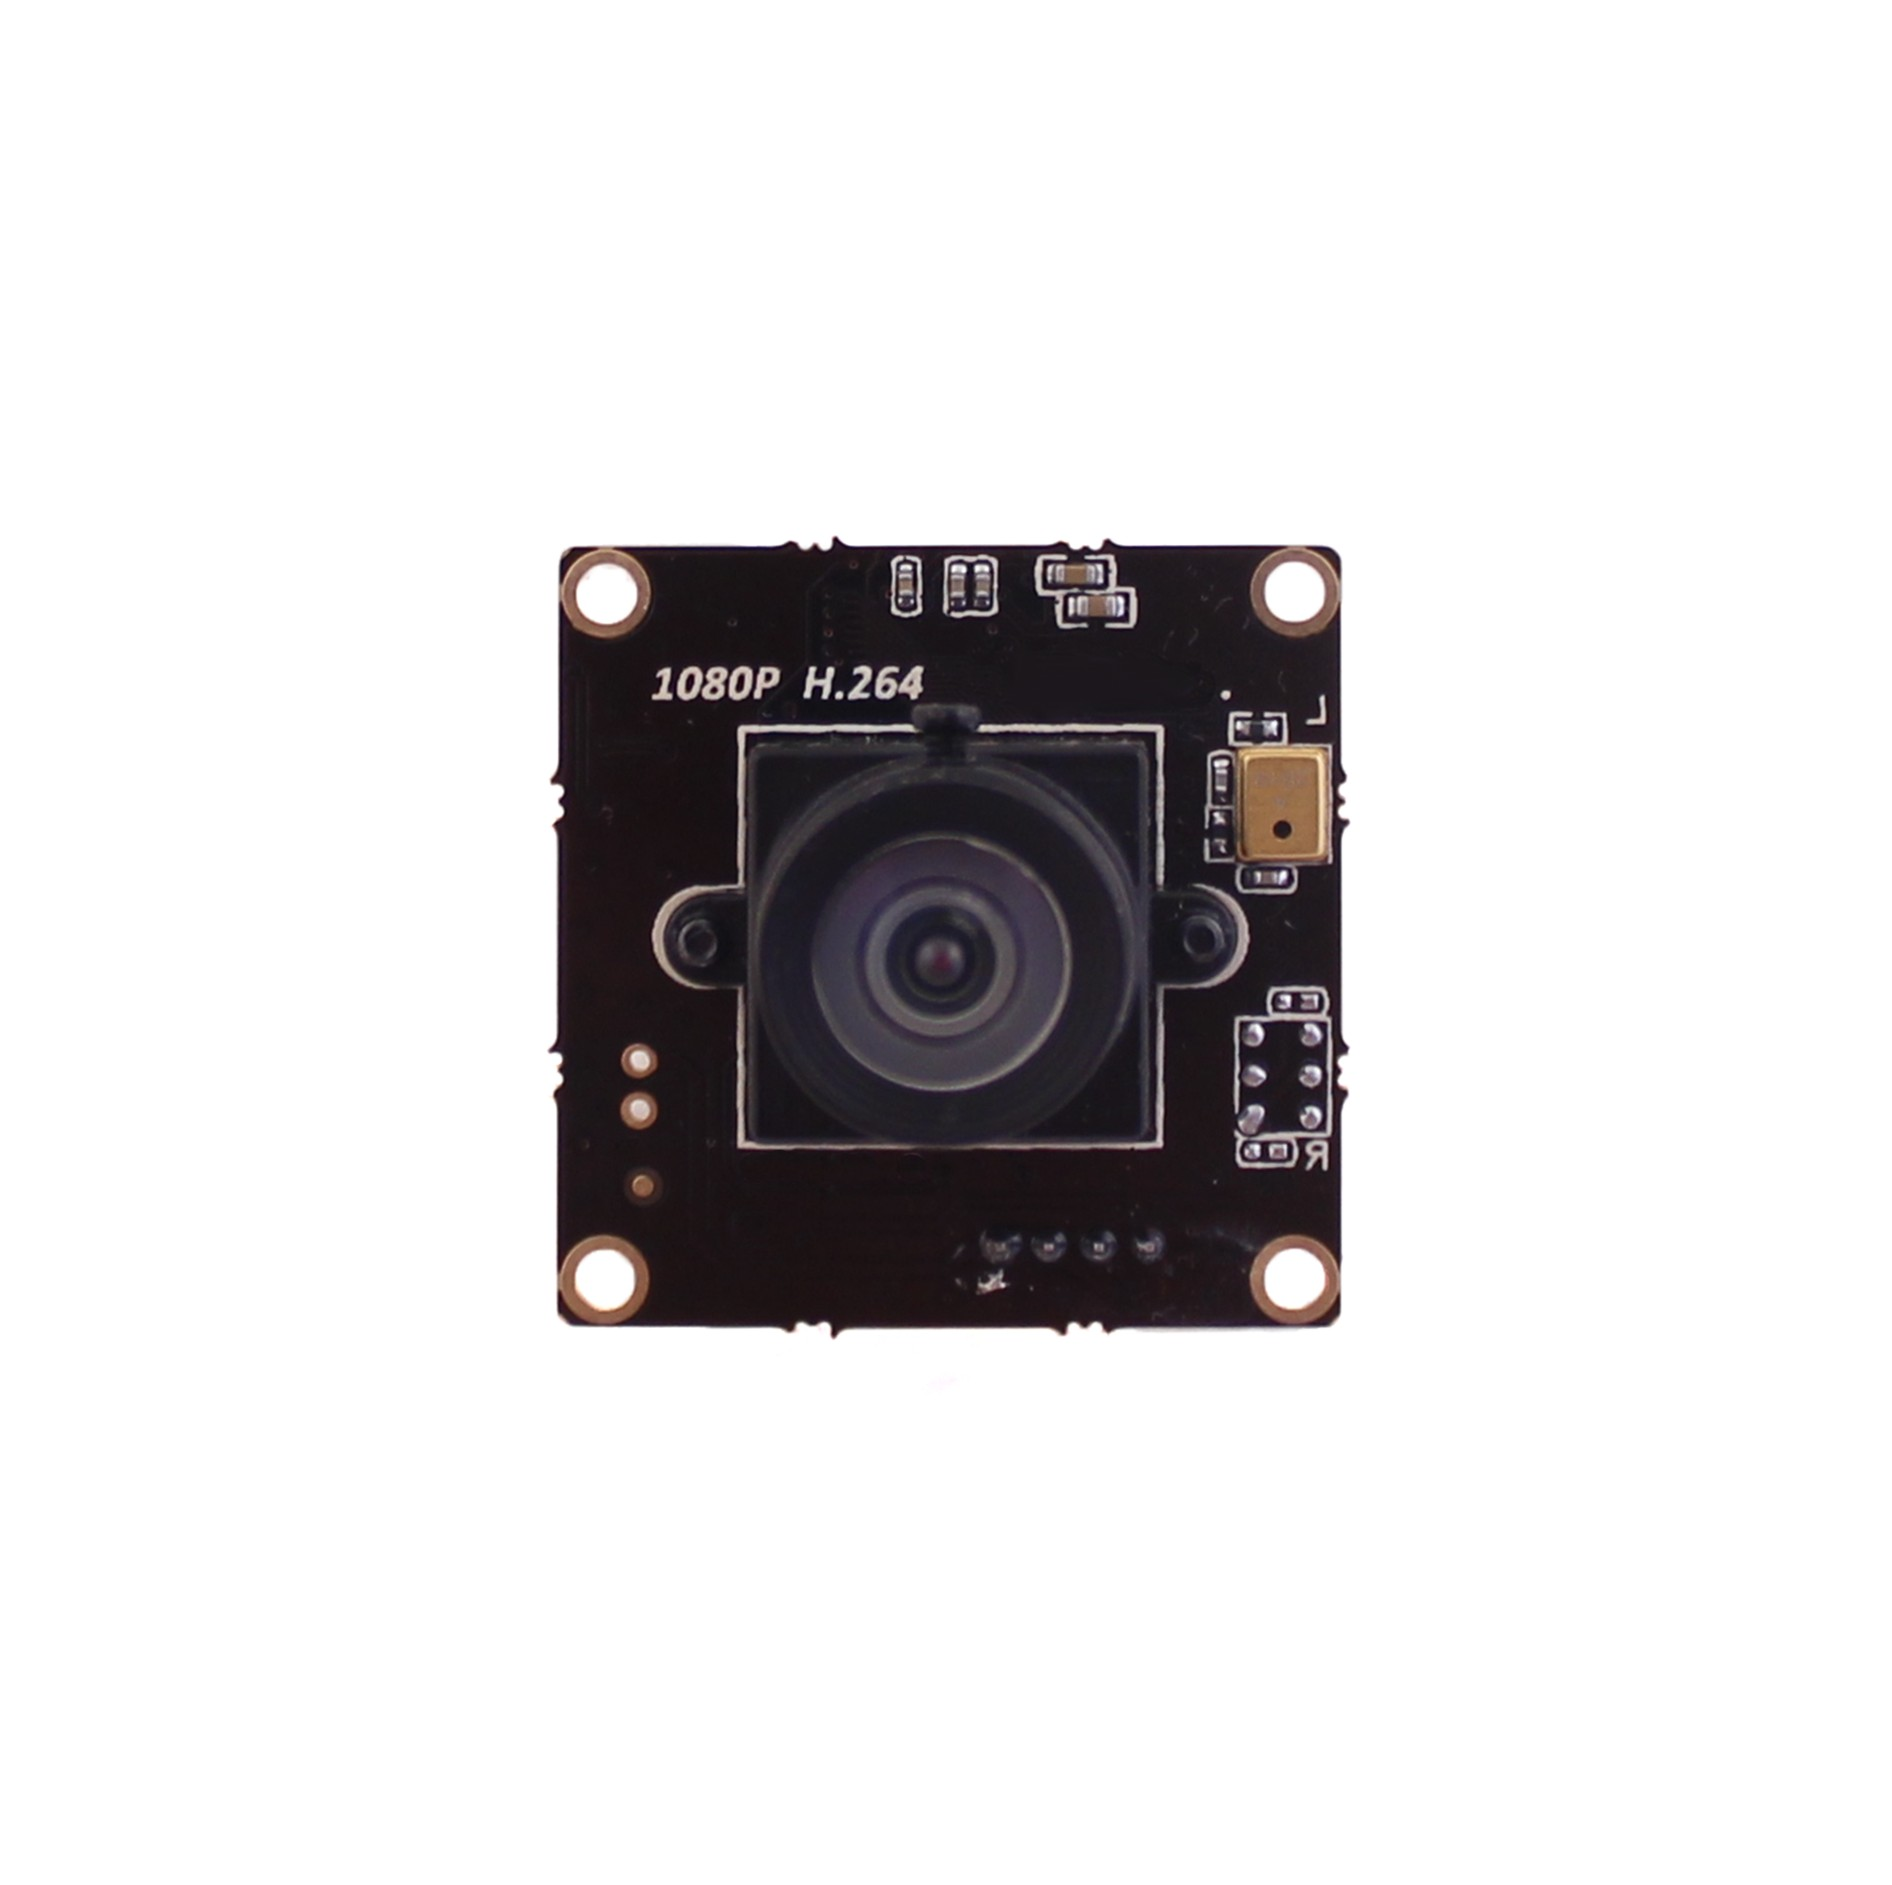
\includegraphics[height=2.2cm, keepaspectratio]{camera_hd.jpg}\\
        \vspace{0.2em}
        \tech{Caméra Low-Light HD (Standard)}\\
        \tiny\textit{Capteur Sony CMOS $\cdot$ $1080\text{p}@30\,\text{fps}$ $\cdot$ $0.01\,\text{lux}$}
      \end{center}
      \scriptsize
      \begin{itemize}
        \item \textbf{Standard BlueROV2} : caméra USB compacte montée sur berceau pivotant commandé par servomoteur PWM.
        \item \textbf{Nacelle tilt motorisée} : orientable de $+45^\circ$ (navigation avant) à $-90^\circ$ (vue benthique au nadir).
        \item \textbf{Basse latence} : flux H.264 temps réel $<120\,\text{ms}$ vers QGroundControl / Cockpit.
        \item Dôme acrylique hémisphérique corrigeant la réfraction.
      \end{itemize}
    \end{column}

    \begin{column}{0.48\textwidth}
      \begin{center}
        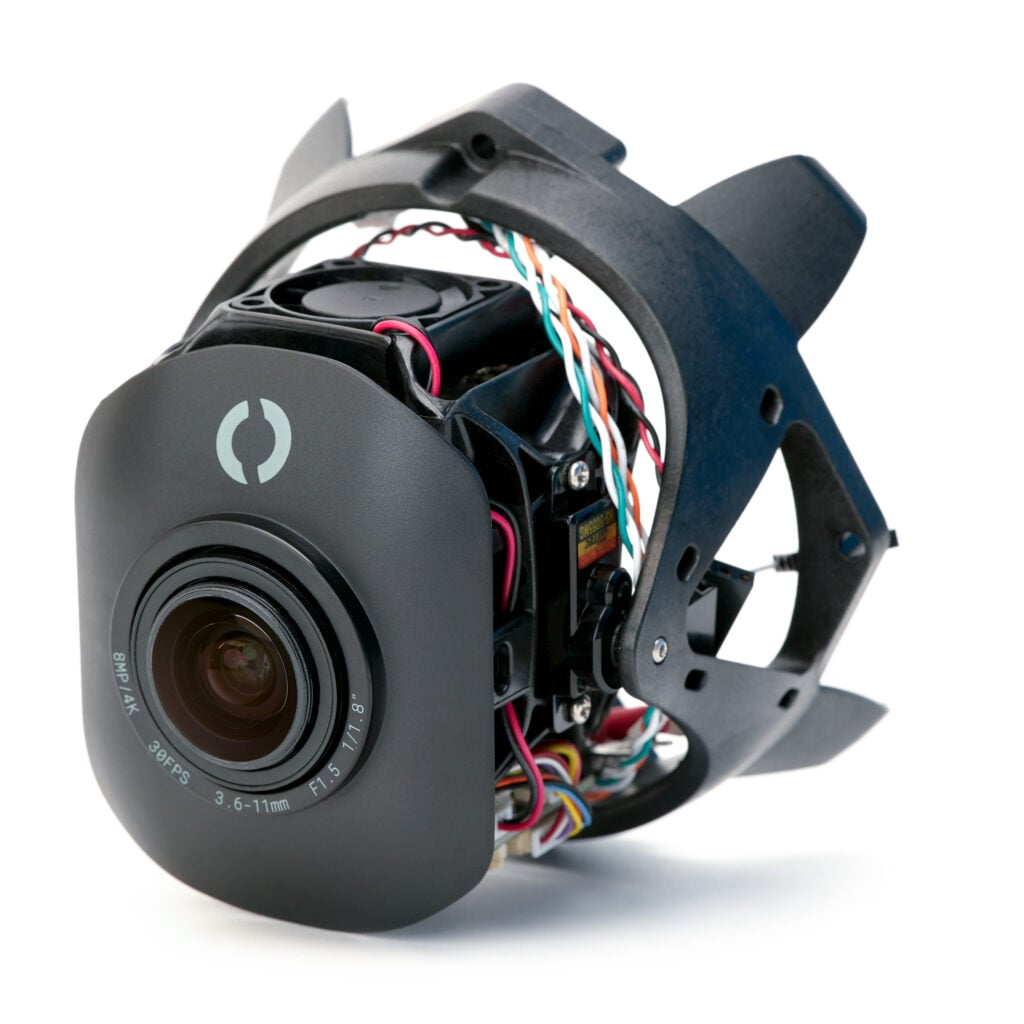
\includegraphics[height=2.2cm, keepaspectratio]{camera_4k.jpg}\\
        \vspace{0.2em}
        \succw{Nouvelle 4K Cam (Ultra-HD \& Zoom)}\\
        \tiny\textit{Capteur Sony Starvis 2 IMX678 $\cdot$ $4\text{K} \ (3840\times 2160)$ $\cdot$ $0.001\,\text{lux}$}
      \end{center}
      \scriptsize
      \begin{itemize}
        \item \textbf{Haute Résolution \& Détails} : $4\times$ plus de pixels pour l'identification taxonomique et la photogrammétrie fine.
        \item \textbf{Optique motorisée} : autofocus rapide et zoom numérique/optique pilotable en direct depuis l'interface Cockpit.
        \item \textbf{Sensibilité extrême} : capteur Starvis 2 rétroéclairé pour les plongées profondes et zones sombres.
        \item Rétrocompatible avec le dôme 4" du BlueROV2.
      \end{itemize}
    \end{column}
  \end{columns}
\end{frame}

\begin{frame}{4.0c Éclairage Étanche \& Échelle : Feux Lumen \& Lasers}
  \begin{columns}[T]
    \begin{column}{0.48\textwidth}
      \begin{center}
        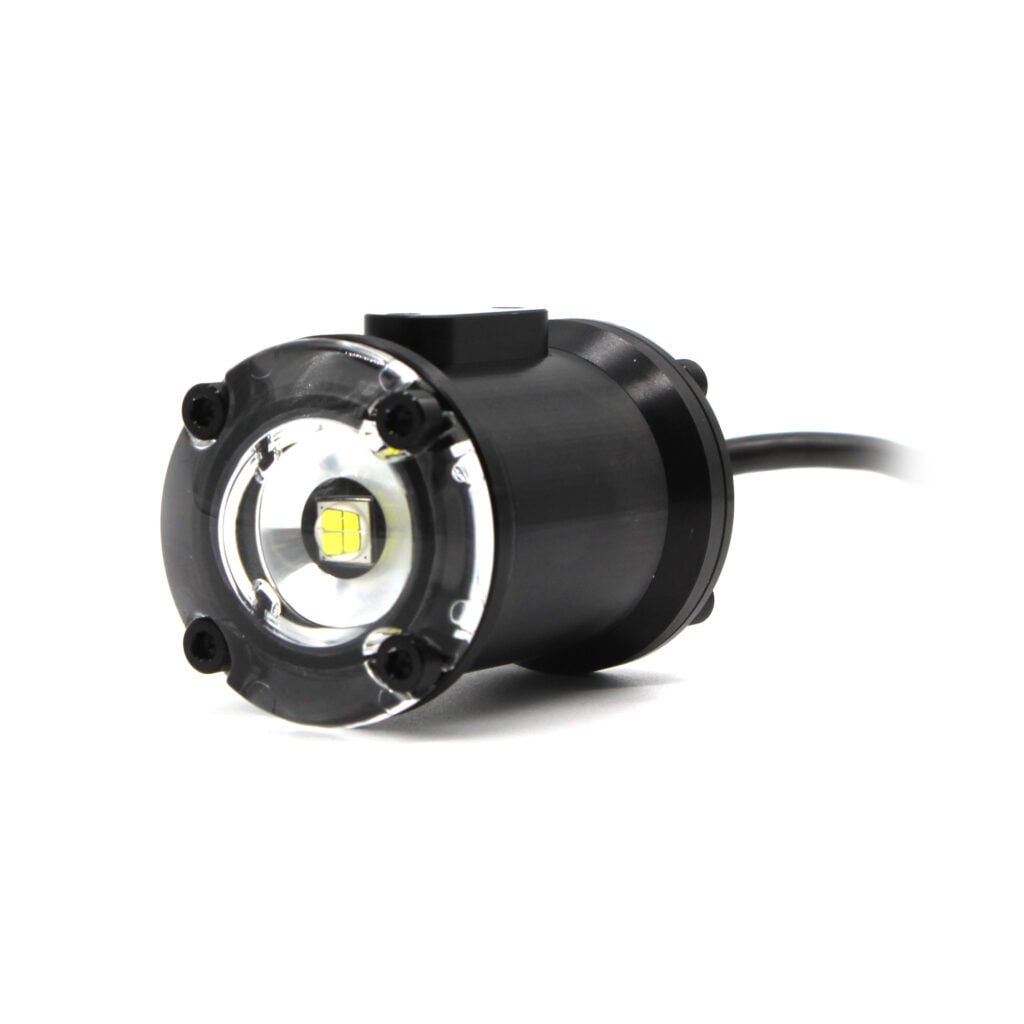
\includegraphics[height=2.2cm, keepaspectratio]{lumen_light.jpg}\\
        \vspace{0.2em}
        \tech{Projecteur Lumen Subsea Light}\\
        \tiny\textit{LED haute puissance $\cdot$ $1500\text{--}6000\,\text{lm}$ $\cdot$ Étanche $500\,\text{m}$ (50 bar)}
      \end{center}
      \scriptsize
      \begin{itemize}
        \item \textbf{Restauration chromatique} : compense la disparition rapide du spectre rouge dès $3\text{--}5\,\text{m}$ de profondeur.
        \item \textbf{Montage déporté vital} : espacé des caméras pour supprimer la rétrodiffusion (*backscatter*) sur la neige marine.
        \item \textbf{Pilotage PWM fin} : intensité variable depuis la manette pour éviter d'éblouir la faune ou saturer l'image.
        \item Balise stroboscopique de repérage en surface.
      \end{itemize}
    \end{column}

    \begin{column}{0.48\textwidth}
      \begin{center}
        \begin{tikzpicture}[scale=0.78]
          % Fond marin
          \draw[thick, fill=brown!20] (-2.2, -1.2) rectangle (2.2, -0.6);
          \node at (0, -0.9) {\tiny Fond benthique / Faune};
          % Cible
          \draw[thick, fill=OceanGreen!40] (-0.8, -0.6) rectangle (0.8, -0.3);
          \node at (0, -0.45) {\tiny Spécimen biologique ($10\,\text{cm}$)};
          % Points laser
          \fill[green!80!black] (-0.5, -0.3) circle (3pt);
          \fill[green!80!black] (0.5, -0.3) circle (3pt);
          \draw[<->, thick, green!70!black] (-0.5, 0.0) -- (0.5, 0.0) node[midway, above] {\tiny $\Delta x = 100\,\text{mm}$ calibré};
          % Faisceaux
          \draw[dashed, green!80!black, line width=1.2pt] (-0.5, 1.4) -- (-0.5, -0.3);
          \draw[dashed, green!80!black, line width=1.2pt] (0.5, 1.4) -- (0.5, -0.3);
          % Boîtier laser
          \draw[thick, fill=OceanDeep!80] (-0.9, 1.4) rectangle (-0.1, 1.8);
          \draw[thick, fill=OceanDeep!80] (0.1, 1.4) rectangle (0.9, 1.8);
          \node[white] at (-0.5, 1.6) {\tiny Laser 1};
          \node[white] at (0.5, 1.6) {\tiny Laser 2};
        \end{tikzpicture}\\
        \vspace{0.2em}
        \alertw{Lasers de Dimensionnement Sous-Marins}\\
        \tiny\textit{Double faisceau vert parallèle $\cdot$ Référence métrique absolue}
      \end{center}
      \scriptsize
      \begin{itemize}
        \item Deux lasers étanches montés à distance rigoureusement fixe ($50$ ou $100\,\text{mm}$).
        \item Projettent 2 points d'échelle métrique directe sans contact sur les captures vidéo (biométrie, géologie).
      \end{itemize}
    \end{column}
  \end{columns}
\end{frame}

\begin{frame}{4.1 Les Sonars Concrets du Chercheur : Ping Sonar \& Ping360}
  \begin{columns}[T]
    \begin{column}{0.48\textwidth}
      \begin{center}
        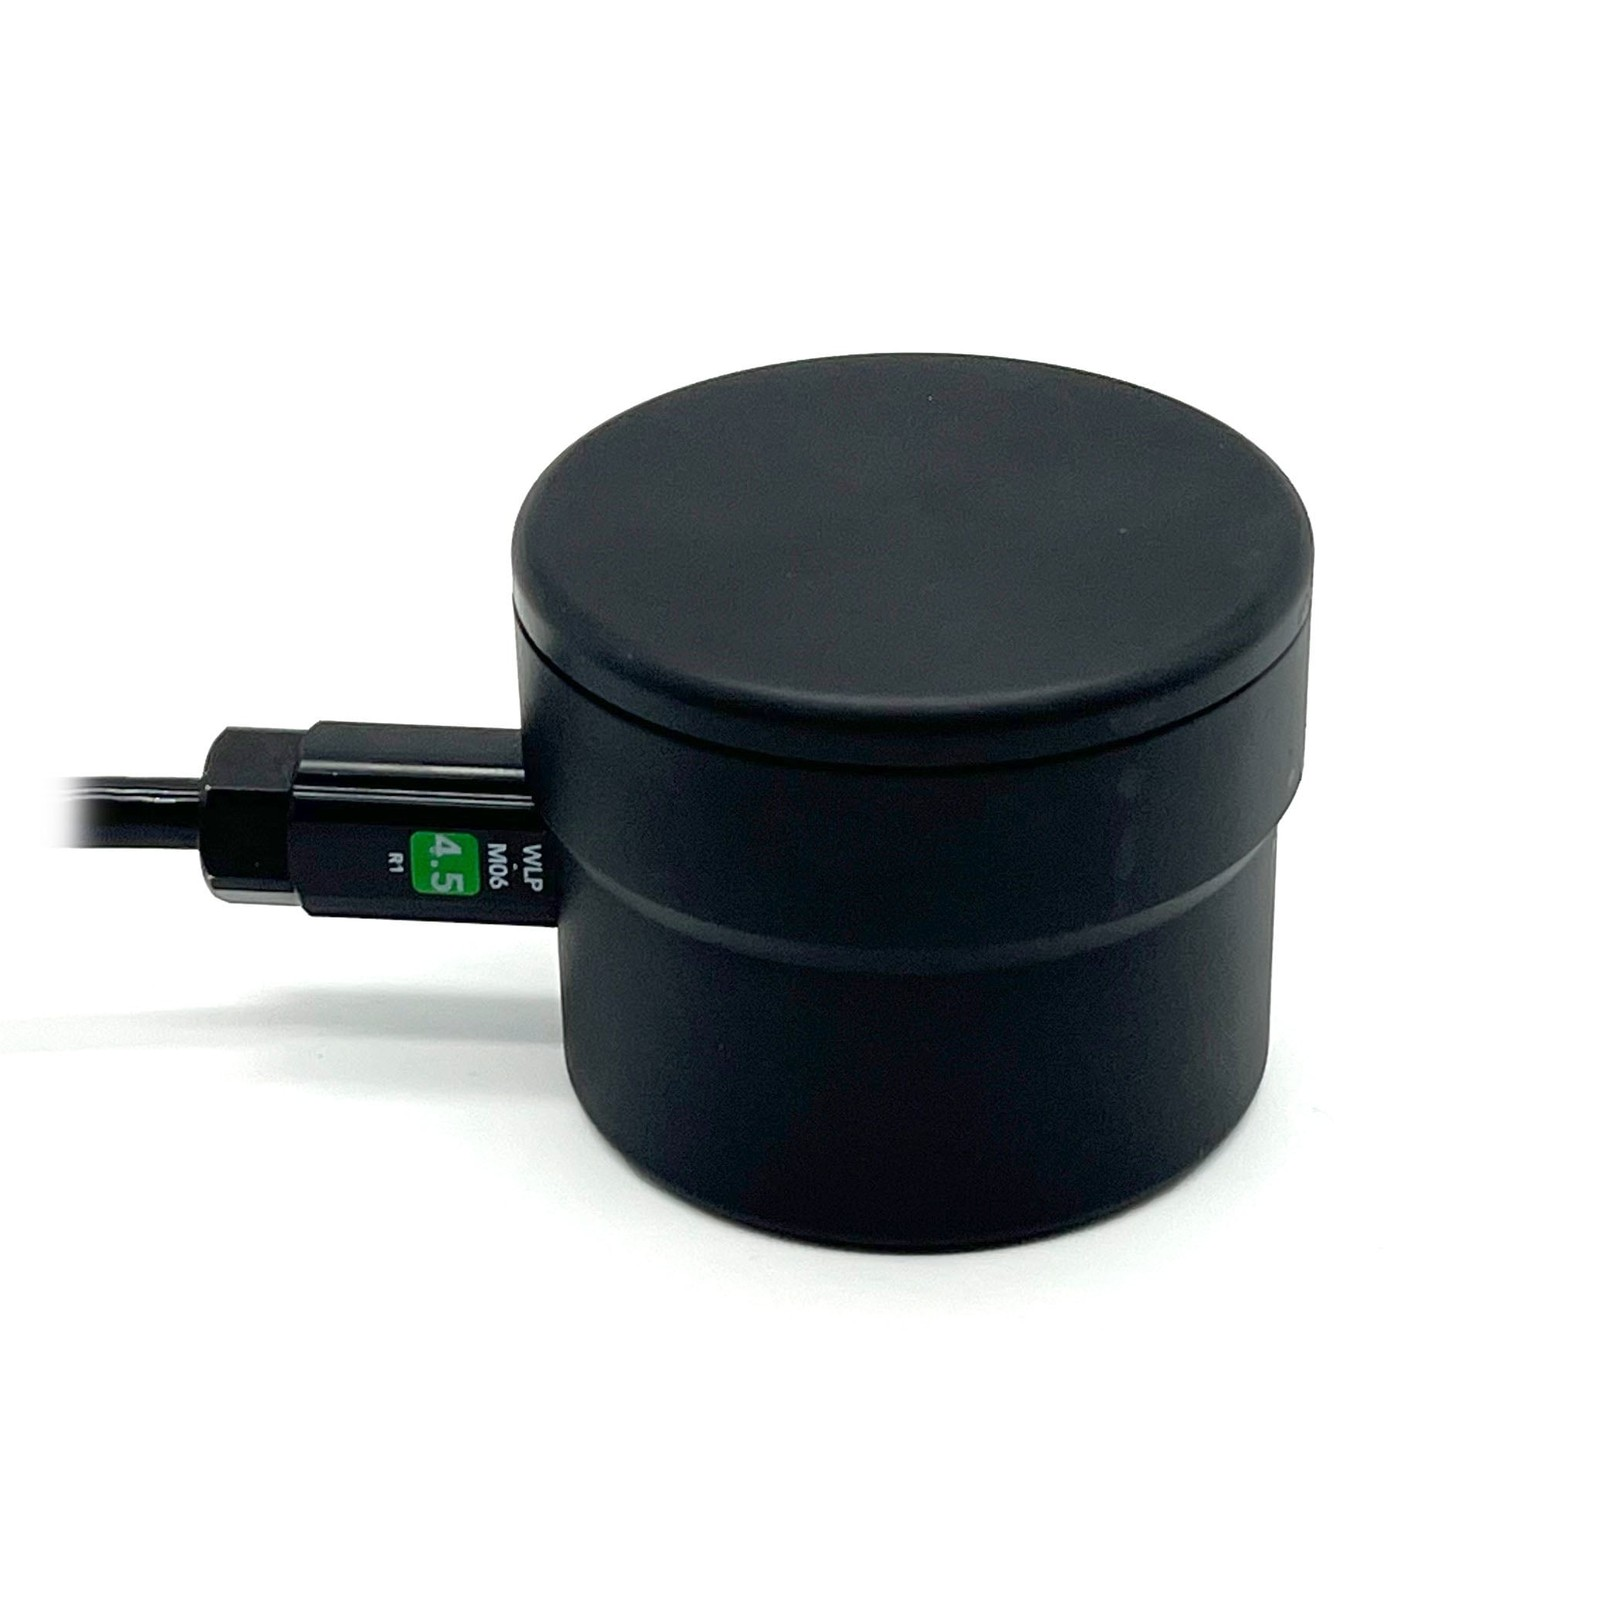
\includegraphics[height=2.3cm, keepaspectratio]{ping_echosounder.jpg}\\
        \vspace{0.2em}
        \tech{Ping Sonar (Échosondeur 115 kHz)}
      \end{center}
      \scriptsize
      \begin{itemize}
        \item \textbf{Principe} : mono-faisceau vertical ($30^\circ$).
        \item Portée : $0.5\,\text{m}$ à $50\,\text{m}$.
        \item Interface : série UART / USB ($115200\,\text{bauds}$).
        \item \textbf{Usages} : altimètre pour \textit{bottom-following} sur ROV et bathymétrie simple sur BlueBoat.
        \item Librairie Python ouverte : \code{ping-python}.
      \end{itemize}
    \end{column}

    \begin{column}{0.48\textwidth}
      \begin{center}
        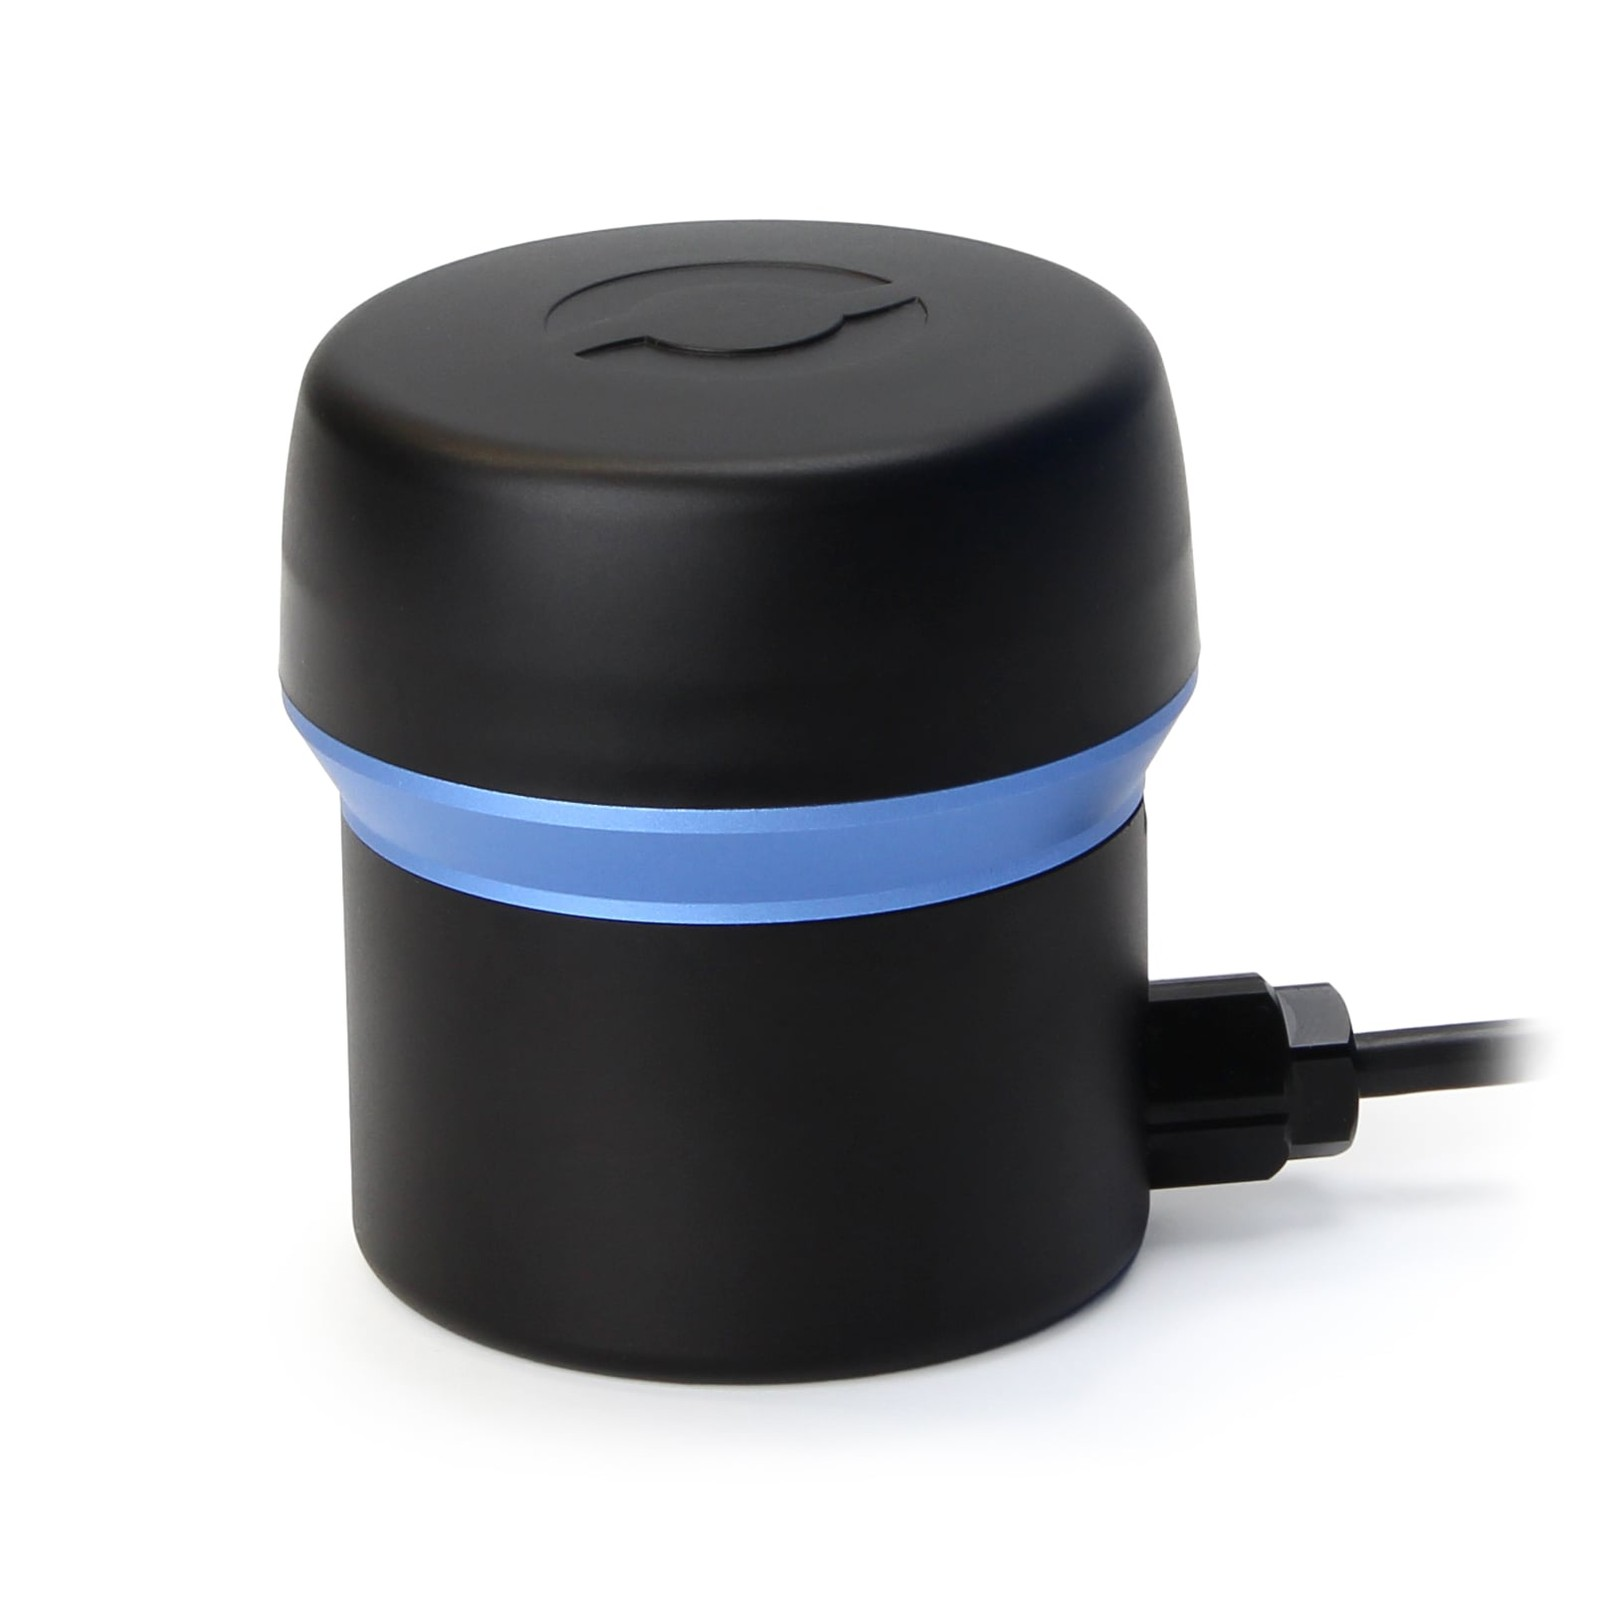
\includegraphics[height=2.3cm, keepaspectratio]{ping360_sonar.jpg}\\
        \vspace{0.2em}
        \tech{Ping360 (Sonar à Balayage 750 kHz)}
      \end{center}
      \scriptsize
      \begin{itemize}
        \item \textbf{Principe} : transducteur piézo rotatif motorisé.
        \item Faisceau fin : $2^\circ$ horizontal $\times 30^\circ$ vertical.
        \item Portée : jusqu'à $50\,\text{m}$ de rayon.
        \item \textbf{Usages} : navigation et évitement d'obstacles en eau turbide, détection de falaises et épaves.
      \end{itemize}
    \end{column}
  \end{columns}
\end{frame}

\begin{frame}{4.1b Imagerie Acoustique \& Sondeur Multifaisceaux (MBES)}
  \begin{columns}[T]
    \begin{column}{0.48\textwidth}
      \begin{center}
        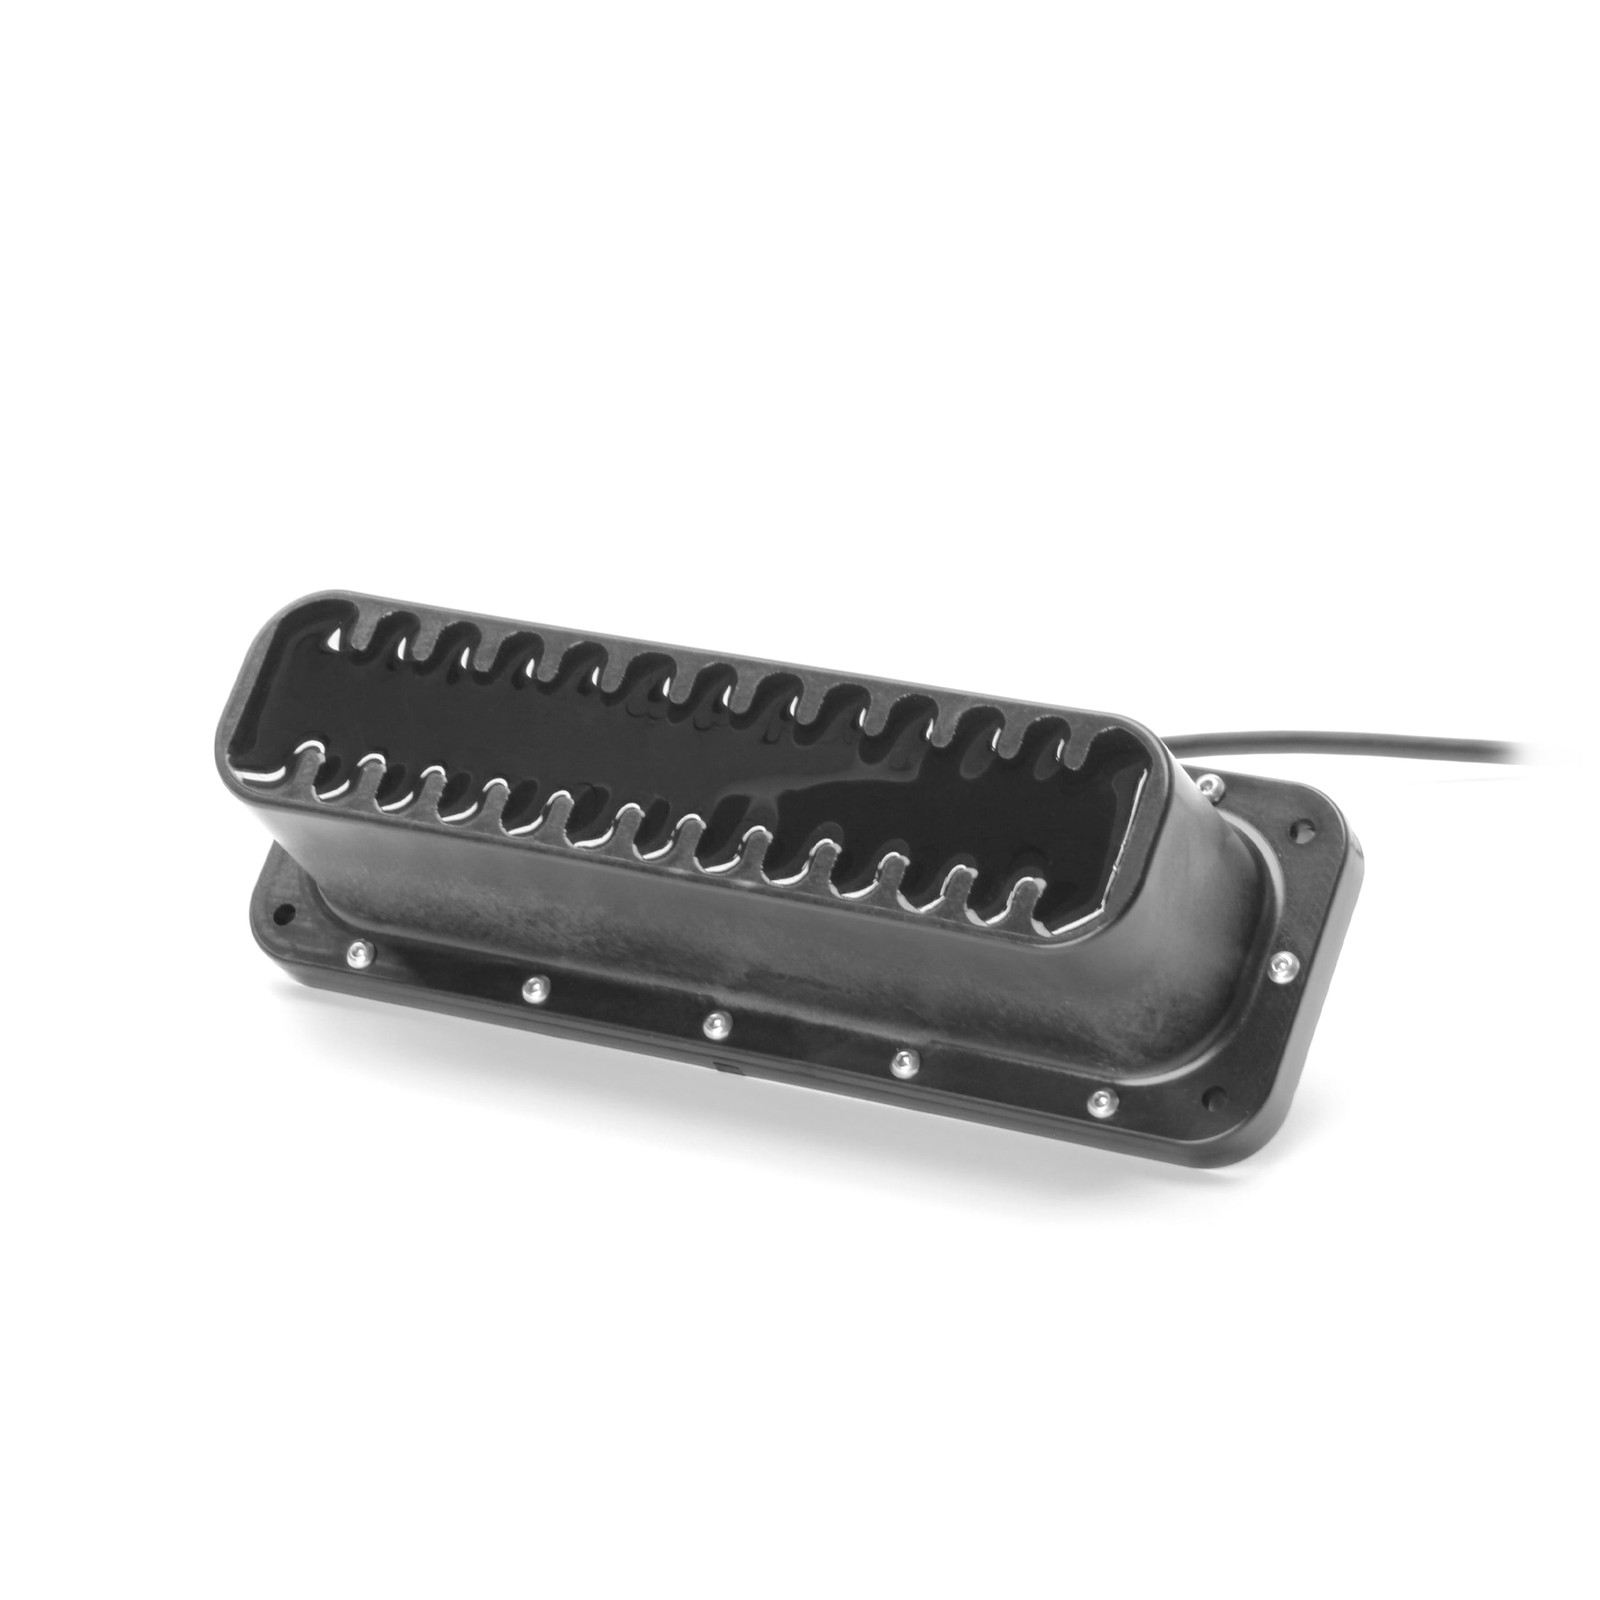
\includegraphics[height=2.4cm, keepaspectratio]{cerulean_omniscan.jpg}\\
        \vspace{0.2em}
        \tech{Cerulean Omniscan 450 FS}\\
        \footnotesize\textbf{Sonar d'Imagerie \& Balayage Avant}
      \end{center}
      \scriptsize
      \begin{itemize}
        \item \textbf{Fréquence} : $450\,\text{kHz}$, portée jusqu'à $100\,\text{m}$.
        \item \textbf{Imagerie acoustique 2D temps réel} : restitution d'échos haute résolution type "caméra acoustique".
        \item \textbf{Applications} : navigation en zéro visibilité, détection d'obstacles et cartographie latérale.
        \item Intégration directe BlueOS \& logiciel \textbf{SonarView}.
      \end{itemize}
    \end{column}

    \begin{column}{0.48\textwidth}
      \begin{center}
        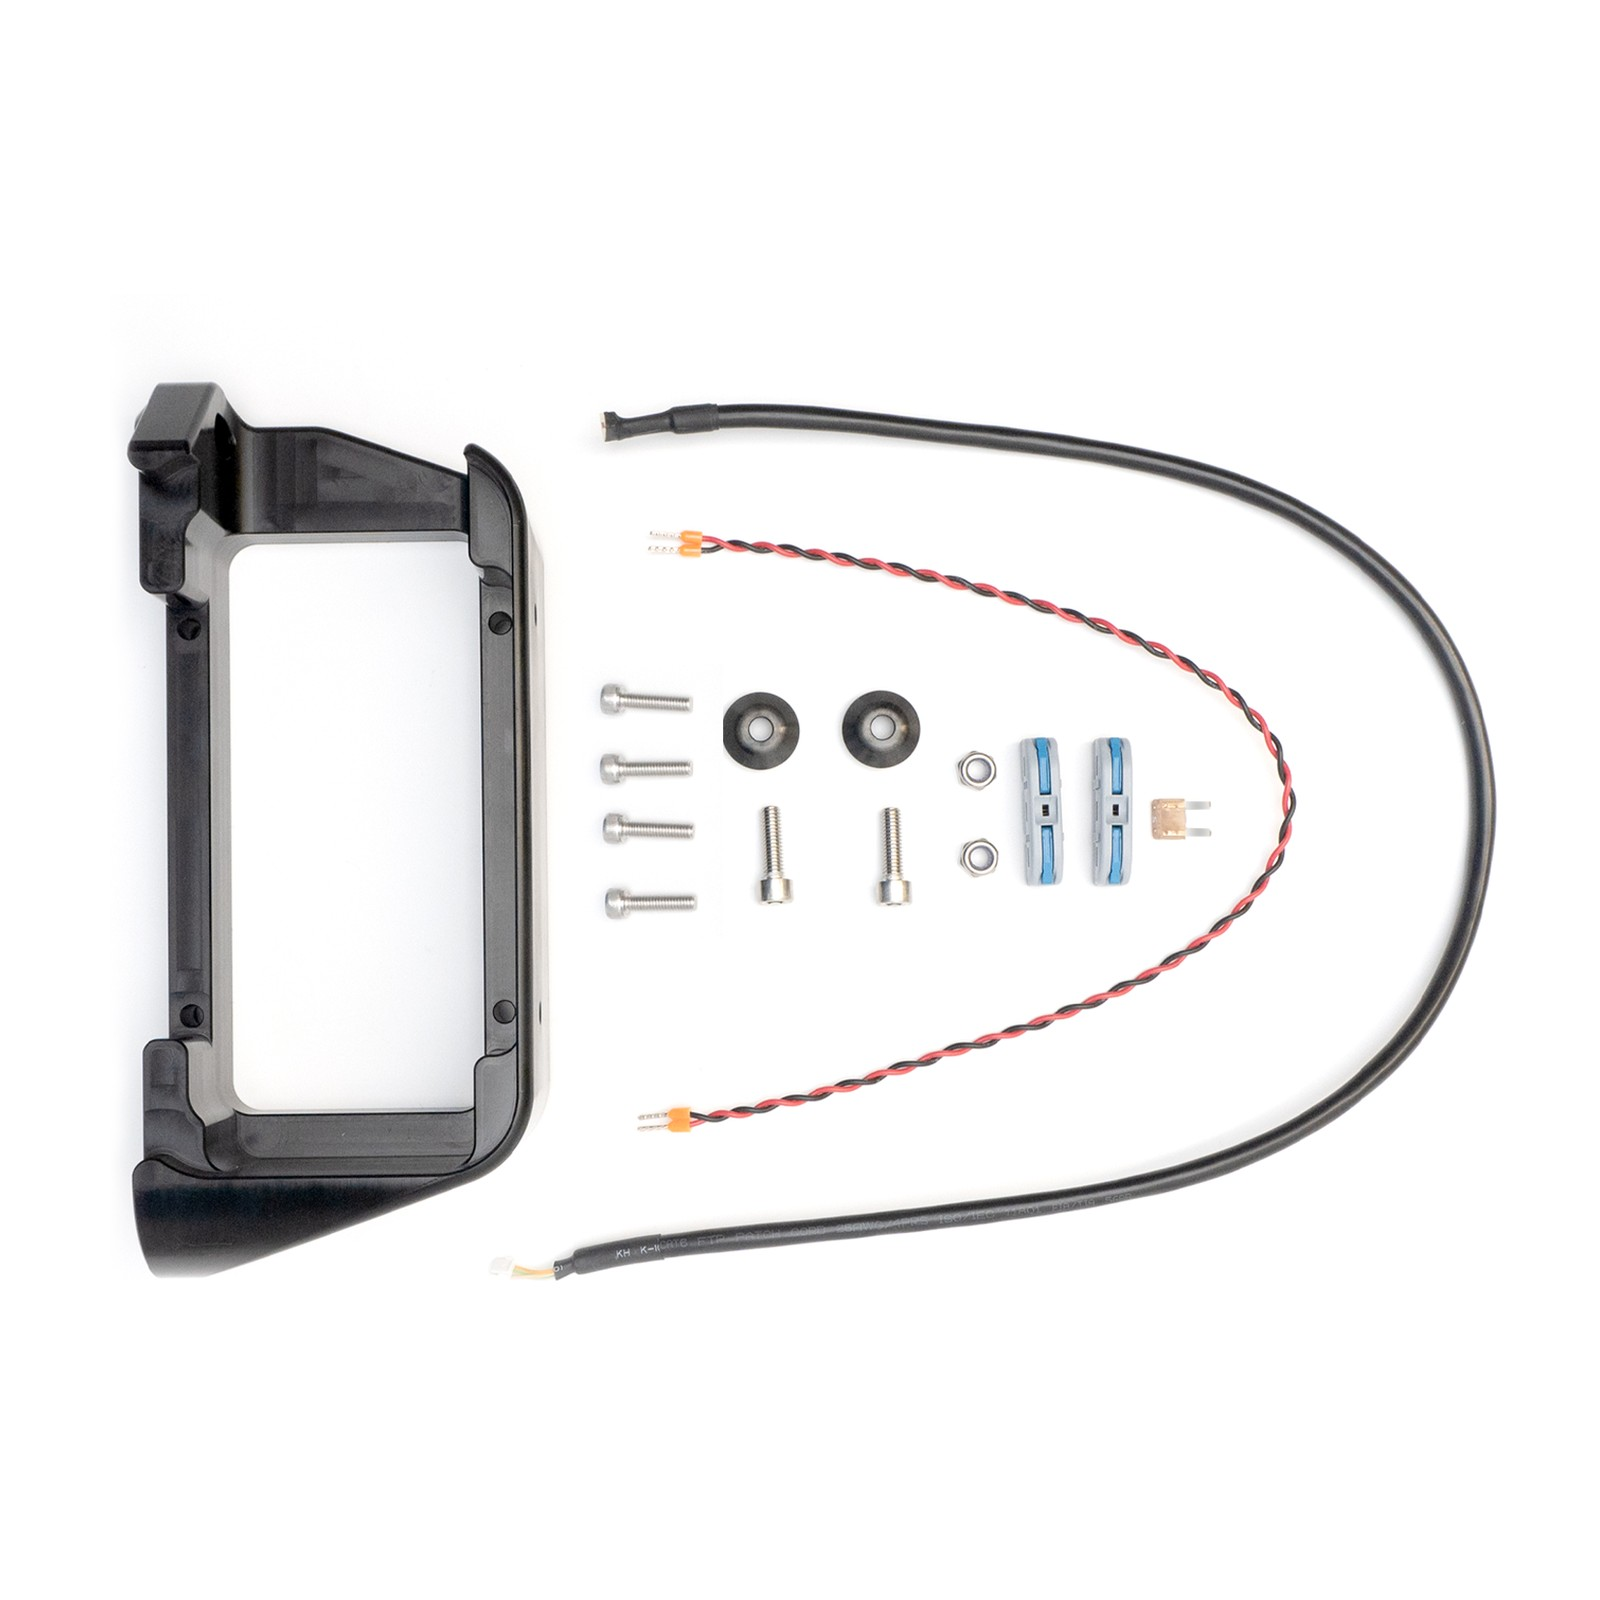
\includegraphics[height=2.4cm, keepaspectratio]{cerulean_surveyor_mbes.jpg}\\
        \vspace{0.2em}
        \tech{Cerulean Surveyor 240-16}\\
        \footnotesize\textbf{Multibeam Echosounder (MBES)}
      \end{center}
      \scriptsize
      \begin{itemize}
        \item \textbf{Multifaisceaux bathymétrique} : $240\,\text{kHz}$, 16 éléments de réception formés numériquement.
        \item \textbf{Fauchée 3D large} : cartographie bathymétrique surfacique (*swath*) haute densité sur \textbf{BlueBoat}.
        \item \textbf{Données denses} : nuages de points 3D couplés au GNSS RTK Centipede.
        \item Démocratisation des levés bathymétriques de laboratoire.
      \end{itemize}
    \end{column}
  \end{columns}
\end{frame}

\begin{frame}{4.2 Le DVL Embarqué : Water Linked DVL-A50}
  \begin{columns}[c]
    \begin{column}{0.54\textwidth}
      \textbf{La démocratisation de l'odométrie sous-marine} :
      \scriptsize
      \begin{itemize}
        \item Le \tech{Water Linked DVL-A50} :
          \begin{itemize}
            \item Poids dans l'eau : seulement \textbf{$270\,\text{g}$} (historiquement $>10\,\text{kg}$).
            \item 4 faisceaux Janus acoustiques à $1\,\text{MHz}$.
            \item Vitesse sol ($0.05\,\text{m}$ à $50\,\text{m}$ d'altitude fond).
          \end{itemize}
        \item \succw{Intégration directe BlueOS / ArduSub} :
          \begin{itemize}
            \item Se branche en Ethernet ou série sur le Raspberry Pi.
            \item Extension BlueOS dédiée disponible en 1 clic.
            \item Active le mode \textbf{Position Hold} : maintien stationnaire automatique face au courant.
          \end{itemize}
      \end{itemize}

      \vspace{0.2em}
      \begin{alertblock}{Usage Réel : Capteur de Navigation (Non Payload)}
        \scriptsize
        \textbf{Rappel important} : Le DVL est un \alertw{capteur de navigation et d'odométrie autonome} (pour l'asservissement en boucle fermée et le maintien de position du véhicule), et \textbf{non une charge utile scientifique} de prélèvement.
      \end{alertblock}
    \end{column}

    \begin{column}{0.44\textwidth}
      \begin{center}
        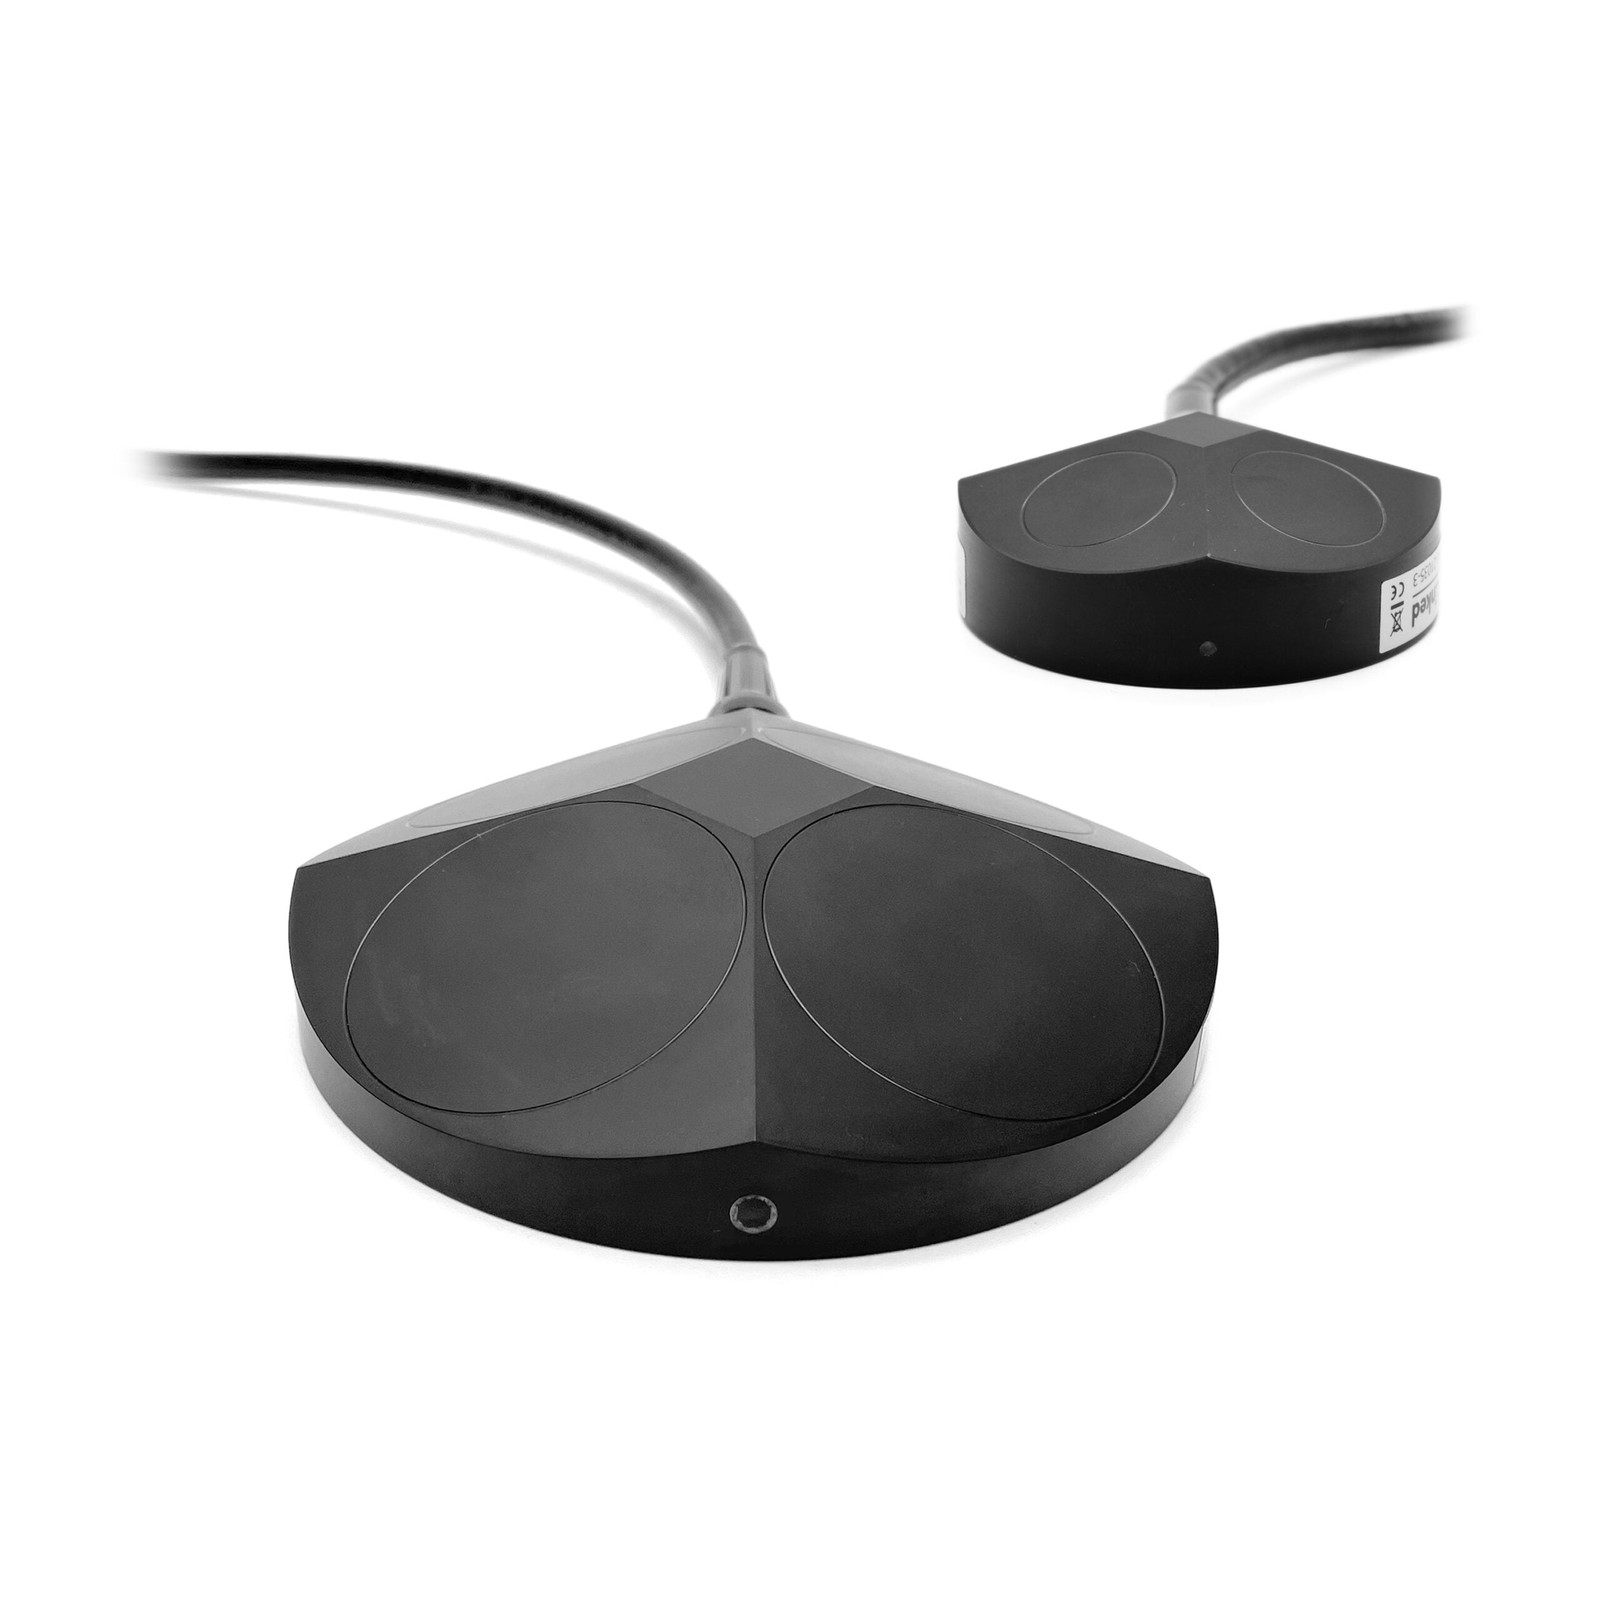
\includegraphics[height=2.3cm, keepaspectratio]{dvl_a50.jpg}\\
        \vspace{0.2em}
        \footnotesize\textbf{Capteur DVL-A50}\\
        \scriptsize\textit{Transducteur 4 faisceaux Janus 1 MHz}
      \end{center}
      \begin{center}
        \begin{tikzpicture}[scale=0.72]
          \draw[thick, fill=OceanMedium!20, rounded corners] (-1.8, 0.8) rectangle (1.8, 1.3);
          \node at (0, 1.05) {\tiny Châssis BlueROV2};
          \draw[thick, fill=black!80] (-0.7, 0.3) rectangle (0.7, 0.8);
          \node[white] at (0, 0.55) {\tiny DVL};
          \draw[->, line width=1.2pt, OceanCyan] (-0.5, 0.3) -- (-1.5, -0.8);
          \draw[->, line width=1.2pt, OceanCyan] (0.5, 0.3) -- (1.5, -0.8);
          \draw[->, line width=1.2pt, OceanMedium] (-0.2, 0.3) -- (-0.6, -0.8);
          \draw[->, line width=1.2pt, OceanMedium] (0.2, 0.3) -- (0.6, -0.8);
          \draw[thick, fill=brown!30] (-2, -0.8) rectangle (2, -1.05);
          \node at (0, -0.92) {\tiny Fond marin (Bottom-Track)};
        \end{tikzpicture}
      \end{center}
    \end{column}
  \end{columns}
\end{frame}

\begin{frame}{4.3 Intégration d'un Capteur Scientifique Tiers}
  \begin{columns}[T]
    \begin{column}{0.49\textwidth}
      \begin{block}{\tech{1. Intégration Mécanique \& Câblage}}
        \scriptsize
        \begin{itemize}
          \item Traversée du caisson : Penetrateur \tech{WetLink M10} ou connecteur débrochable (\tech{Cobalt} / \tech{SubConn}).
          \item Raccordement interne sur le \textbf{Raspberry Pi} :
            \begin{itemize}\tiny
              \item Port USB via convertisseur série RS-232 / RS-485 isolé.
              \item Bus I2C / SPI / ADC sur la carte Navigator.
            \end{itemize}
        \end{itemize}
      \end{block}
    \end{column}

    \begin{column}{0.49\textwidth}
      \begin{block}{\succw{2. Flux Logiciel sous BlueOS}}
        \scriptsize
        \begin{itemize}
          \item Démon Python lisant les trames du capteur (température, DO, turbidité).
          \item \succw{Temps réel surface} : envoi MAVLink \code{NAMED\_VALUE\_FLOAT} pour affichage dans \textbf{Cockpit}.
          \item \succw{Post-mission} : CSV local ou topics \textbf{ROS 2} enregistrés en \code{rosbag2}.
        \end{itemize}
      \end{block}
    \end{column}
  \end{columns}
\end{frame}

\begin{frame}{4.4 Le C{\oe}ur Océanographique : La Mesure CTD}
  \begin{columns}[c]
    \begin{column}{0.55\textwidth}
      \textbf{CTD : \textit{Conductivity - Temperature - Depth}}
      \begin{itemize}
        \item \textbf{Conductivité} : cellule inductive ou à électrodes.
        \item \textbf{Température} : thermistance étalonnée (précision $<0.01^\circ\text{C}$).
        \item \textbf{Pression} : assurée directement par le capteur \tech{Bar30} !
      \end{itemize}

      \vspace{0.4em}
      \begin{block}{Paramètres Dérivés Fondamentaux (TEOS-10)}
        \begin{itemize}
          \item \textbf{Salinité absolue} $S_A$ ($\text{g/kg}$ ou PSU).
          \item \textbf{Masse volumique} $\rho(S, T, P)$.
          \item \tech{Célérité du son} $c(S, T, P)$ : \textbf{indispensable} pour corriger la portée des sonars et de l'USBL !
        \end{itemize}
      \end{block}
    \end{column}

    \begin{column}{0.45\textwidth}
      \begin{center}
        \begin{tikzpicture}[scale=0.85]
          \draw[->] (0,0) -- (3.5,0) node[right] {\small $T, S, \rho$};
          \draw[->] (0,0) -- (0,-3.5) node[below] {\small Profondeur $z$};
          
          \draw[thick, OceanCoral] (3, 0) -- (3, -0.8) to[out=-90, in=90] (0.8, -2.2) -- (0.7, -3.4) node[right] {\small $T^\circ\text{C}$};
          \node[OceanCoral, right] at (1.8,-1.5) {\footnotesize Thermocline};
          
          \draw[thick, OceanCyan] (0.8, 0) -- (0.8, -0.8) to[out=-90, in=90] (2.8, -2.2) -- (2.9, -3.4) node[right] {\small $\rho$};
          \node[OceanCyan, left] at (2.2,-1.5) {\footnotesize Pycnocline};
        \end{tikzpicture}
      \end{center}
      \small
      Le gradient de célérité du son $c(z)$ réfracte les ondes acoustiques.
    \end{column}
  \end{columns}
\end{frame}

\begin{frame}{4.5 Photogrammétrie Benthique avec BlueROV2}
  \begin{columns}[T]
    \begin{column}{0.52\textwidth}
      \textbf{Équipement requis pour le relevé 3D} :
      \begin{itemize}
        \item \textbf{Caméra HD Low-Light} intégrée ou caméra reflex/action cam (GoPro / Sony RX0) dans un caisson dédié.
        \item \textbf{Projecteurs Lumen (BlueRobotics)} : $2 \times 1500\,\text{lumens}$ ou plus, montés aux extrémités du châssis (pour limiter la rétrodiffusion de la neige marine).
        \item Contrôle de l'altitude via le Ping Sonar ou DVL ($1.5\text{--}2.0\,\text{m}$ du fond).
        \item Recouvrement inter-images $>75\%$ en marche avant.
      \end{itemize}
    \end{column}

    \begin{column}{0.48\textwidth}
      \begin{block}{Chaîne de Traitement 3D}
        \begin{itemize}
          \item Extraction des images et synchronisation avec la trajectoire DVL/USBL.
          \item Logiciels SfM : \textbf{Agisoft Metashape}, \textbf{Meshroom} ou \textbf{CloudCompare}.
          \item Correction de la distorsion optique induite par le dôme acrylique.
          \item \succw{Résultat} : orthomosaïque géoréférencée centimétrique et modèle numérique d'élévation (MNE) 3D d'herbiers ou de récifs.
        \end{itemize}
      \end{block}
    \end{column}
  \end{columns}
\end{frame}

\begin{frame}{4.6 Du Signal Brut au Format Standard Océano : NetCDF \& GeoTIFF}
  \begin{center}
    \begin{tikzpicture}[scale=0.85, auto, node distance=1.3cm, >=Latex]
      \node[draw=OceanDeep, fill=OceanDeep!10, rounded corners, rectangle, minimum width=2.6cm, align=center] (raw_nav) {
        \textbf{Navigation}\\
        \footnotesize IMU + DVL + Bar30
      };
      \node[draw=OceanCoral, fill=OceanCoral!10, rounded corners, rectangle, minimum width=2.6cm, align=center, below=0.7cm of raw_nav] (usbl) {
        \textbf{Fixes Acoustiques}\\
        \footnotesize USBL surface + GNSS
      };
      \node[draw=OceanMedium, fill=OceanMedium!20, rounded corners, rectangle, minimum width=3.2cm, align=center, right=1.2cm of raw_nav] (smooth) {
        \textbf{Fusion \& Interpolation}\\
        \footnotesize Trajectoire 4D $(x,y,z,t)$
      };
      \node[draw=OceanGreen, fill=OceanGreen!10, rounded corners, rectangle, minimum width=2.6cm, align=center, above=0.7cm of smooth] (sensors) {
        \textbf{Mesures Capteurs}\\
        \footnotesize CTD, Fluorimètre, Sonar
      };
      \node[draw=OceanCyan, fill=OceanCyan!20, line width=1.5pt, rounded corners, rectangle, minimum width=3.2cm, align=center, right=1.2cm of smooth] (data_product) {
        \textbf{Produit FAIR Final}\\
        \footnotesize \textbf{NetCDF-4} (CF Metadata)\\
        \footnotesize GeoTIFF, Nuage LAS
      };

      \draw[->, thick, OceanDeep] (raw_nav) -- (smooth);
      \draw[->, thick, OceanCoral] (usbl) -| (smooth);
      \draw[->, thick, OceanGreen] (sensors) -- (smooth);
      \draw[->, line width=1.5pt, OceanCyan] (smooth) -- (data_product);
    \end{tikzpicture}
  \end{center}

  \begin{block}{Les Bonnes Pratiques FAIR (Findable, Accessible, Interoperable, Reusable)}
    \begin{itemize}
      \item Enregistrer les métadonnées dès l'acquisition (identifiant du vecteur, étalonnage de la sonde, opérateur).
      \item Utiliser les conventions CF (\textit{Climate and Forecast}) pour que vos données soient directement lisibles par les outils d'analyse (Python \code{xarray}, Ocean Data View, QGIS).
    \end{itemize}
  \end{block}
\end{frame}

% ==============================================================================
% 05_synthese_discussion.tex - Module 5 (16h30 - 17h30)
% Question / discussion & Atelier d'ingénierie projet
% Cas concrets : BlueROV2 échantillonneur, BlueBoat bathymétrique, budget labo, règles d'or
% ==============================================================================

\section{Module 5 : Synthèse \& Discussions}

\begin{frame}{5.1 Cas Pratique 1 : Le BlueROV2 Échantillonneur Benthique}
  \begin{columns}[c]
    \begin{column}{0.35\textwidth}
      \begin{center}
        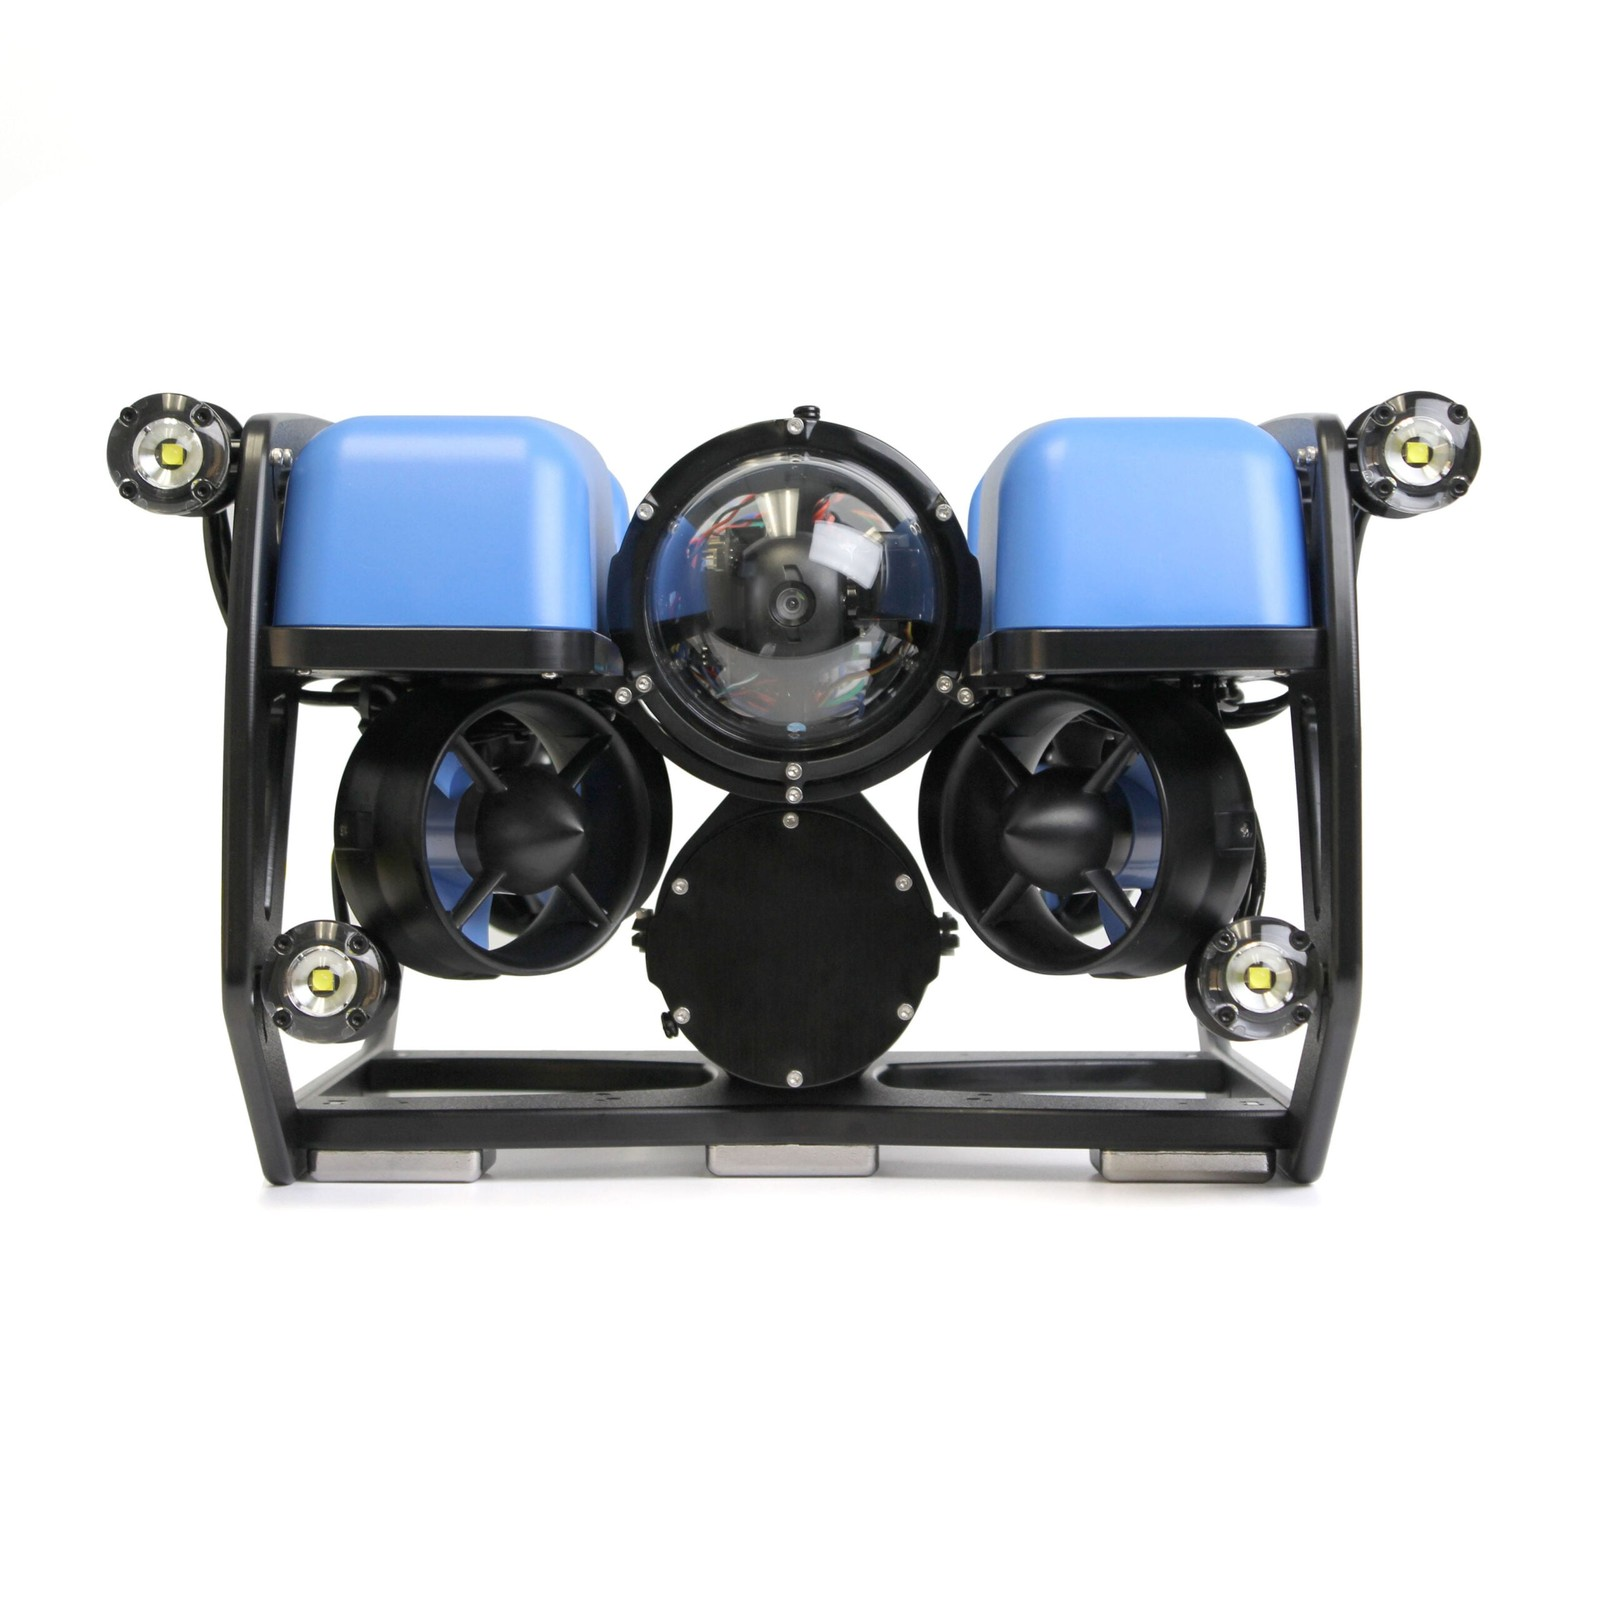
\includegraphics[height=2.0cm, keepaspectratio]{bluerov2.jpg}\\
        \vspace{0.15em}
        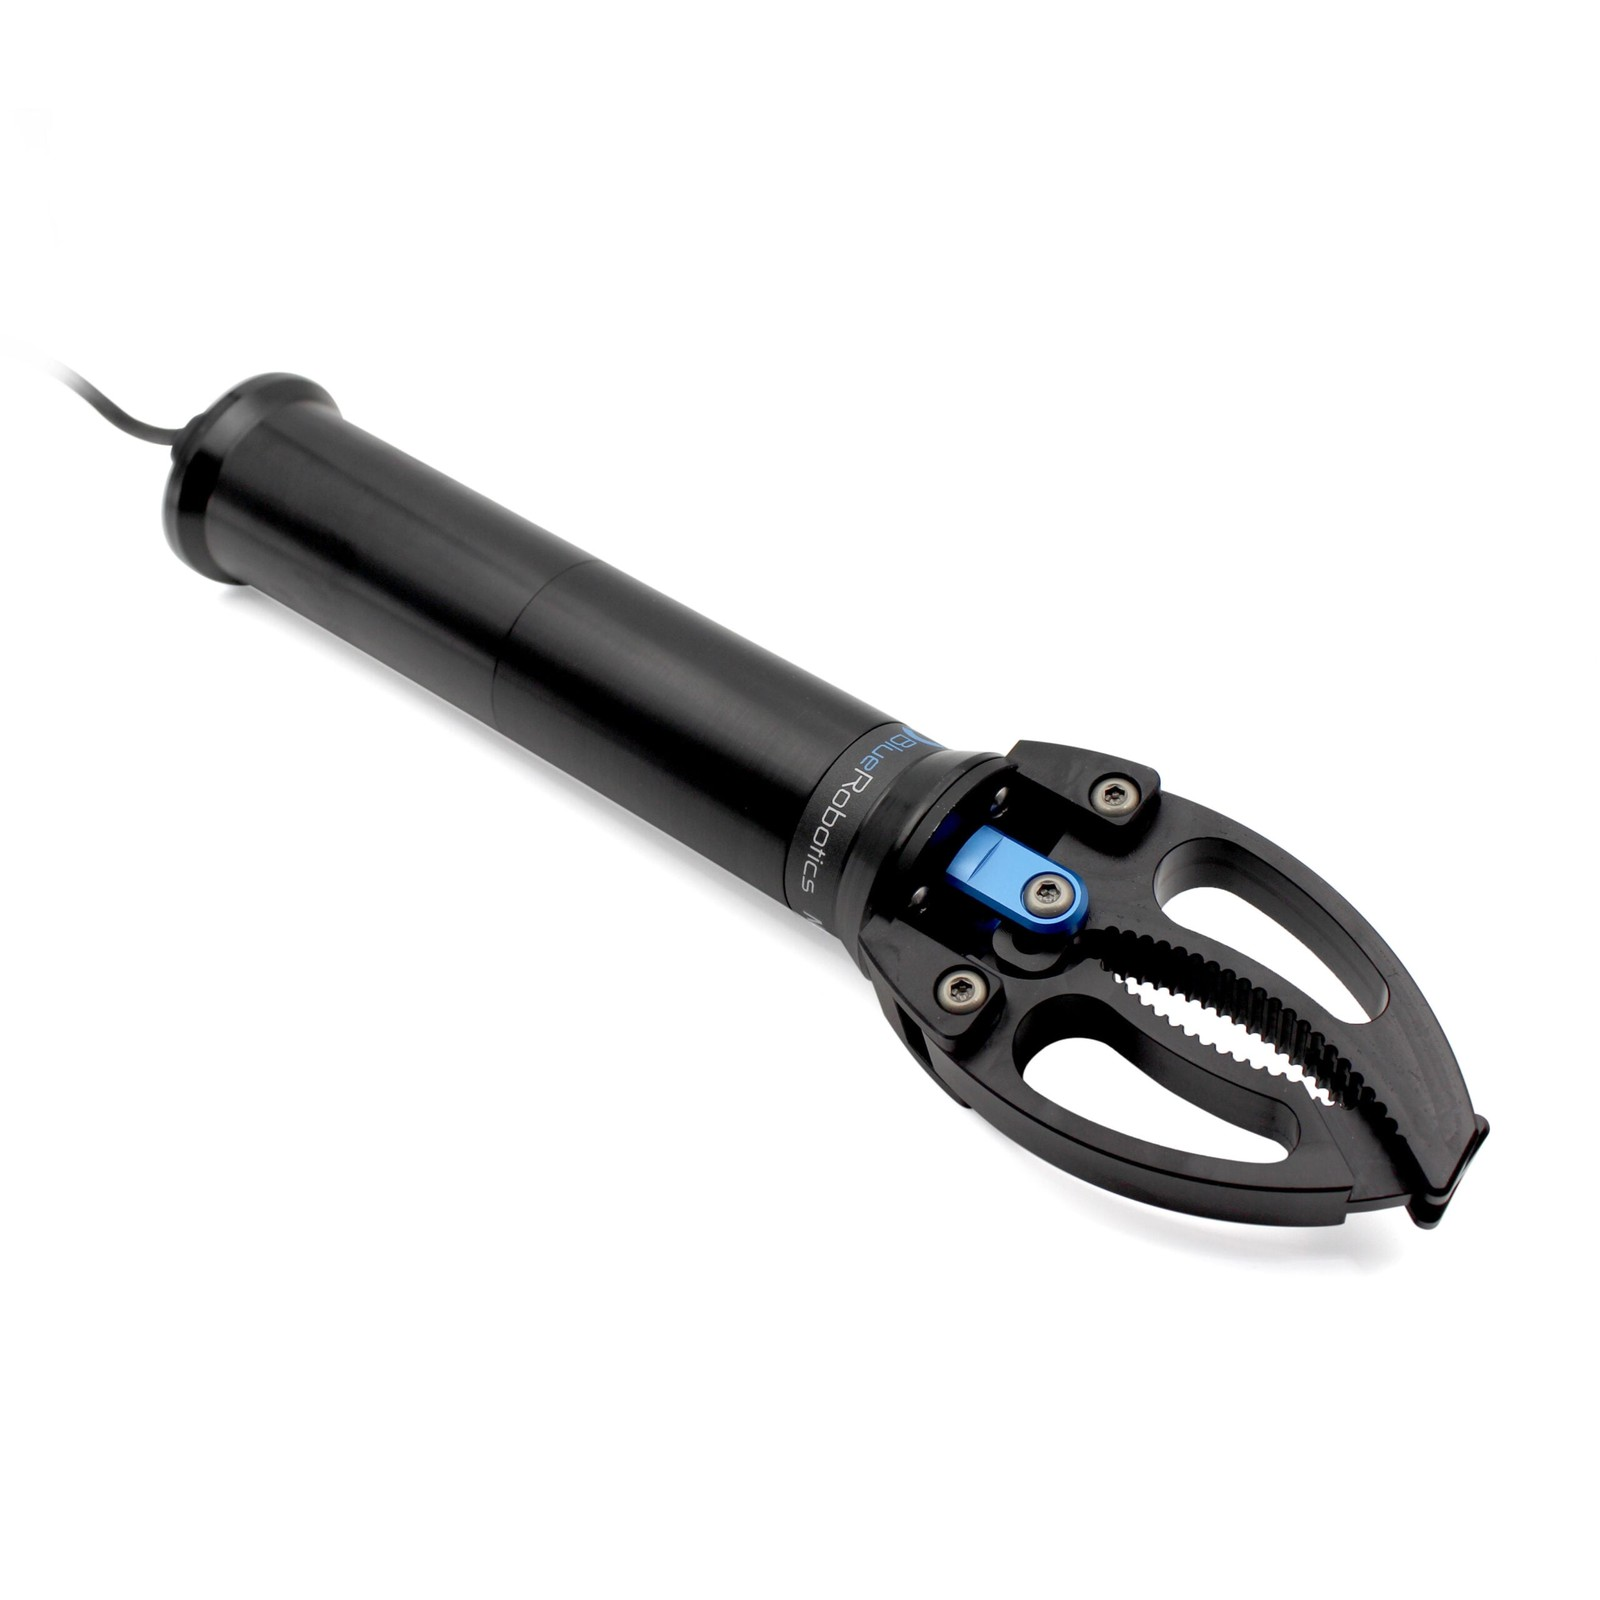
\includegraphics[height=1.7cm, keepaspectratio]{newton_gripper.jpg}\\
        \vspace{0.1em}
        \scriptsize\textbf{BlueROV2 Heavy} + \textbf{Pince Newton}
      \end{center}
    \end{column}

    \begin{column}{0.62\textwidth}
      \textbf{Architecture pour le laboratoire} :
      \scriptsize
      \begin{itemize}
        \item \textbf{Châssis 8 propulseurs (Heavy)} : contrôle complet à 6 DDL, assiette inclinée maintenue vers le fond.
        \item \textbf{Pince Newton Gripper} : préhension d'échantillons géologiques, macroalgues ou pose d'instruments.
        \item \succw{Astuce Caisson Auxiliaire 3"} : caisson 4" réservé à la navigation (jamais ouvert en mer), charge utile scientifique logée dans un caisson 3" dédié.
        \item 4 projecteurs Lumens ($6000\,\text{lm}$) pour vidéo benthique HD.
      \end{itemize}

      \vspace{0.3em}
      \begin{block}{Budget Estimatif Recherche}
        \scriptsize
        BlueROV2 Heavy ($\approx 5\text{--}7\,\text{k€}$) + Pince Newton ($\approx 700\,\text{€}$) + DVL-A50 optionnel ($\approx 6\text{--}8\,\text{k€}$).\\
        \textbf{Total} : $\approx 6\text{--}15\,\text{k€}$ contre $>40\,\text{k€}$ pour un ROV industriel fermé !
      \end{block}
    \end{column}
  \end{columns}
\end{frame}

\begin{frame}{5.2 Cas Pratique 2 : Le BlueBoat Hydrographe \& Qualité d'Eau}
  \begin{columns}[c]
    \begin{column}{0.35\textwidth}
      \begin{center}
        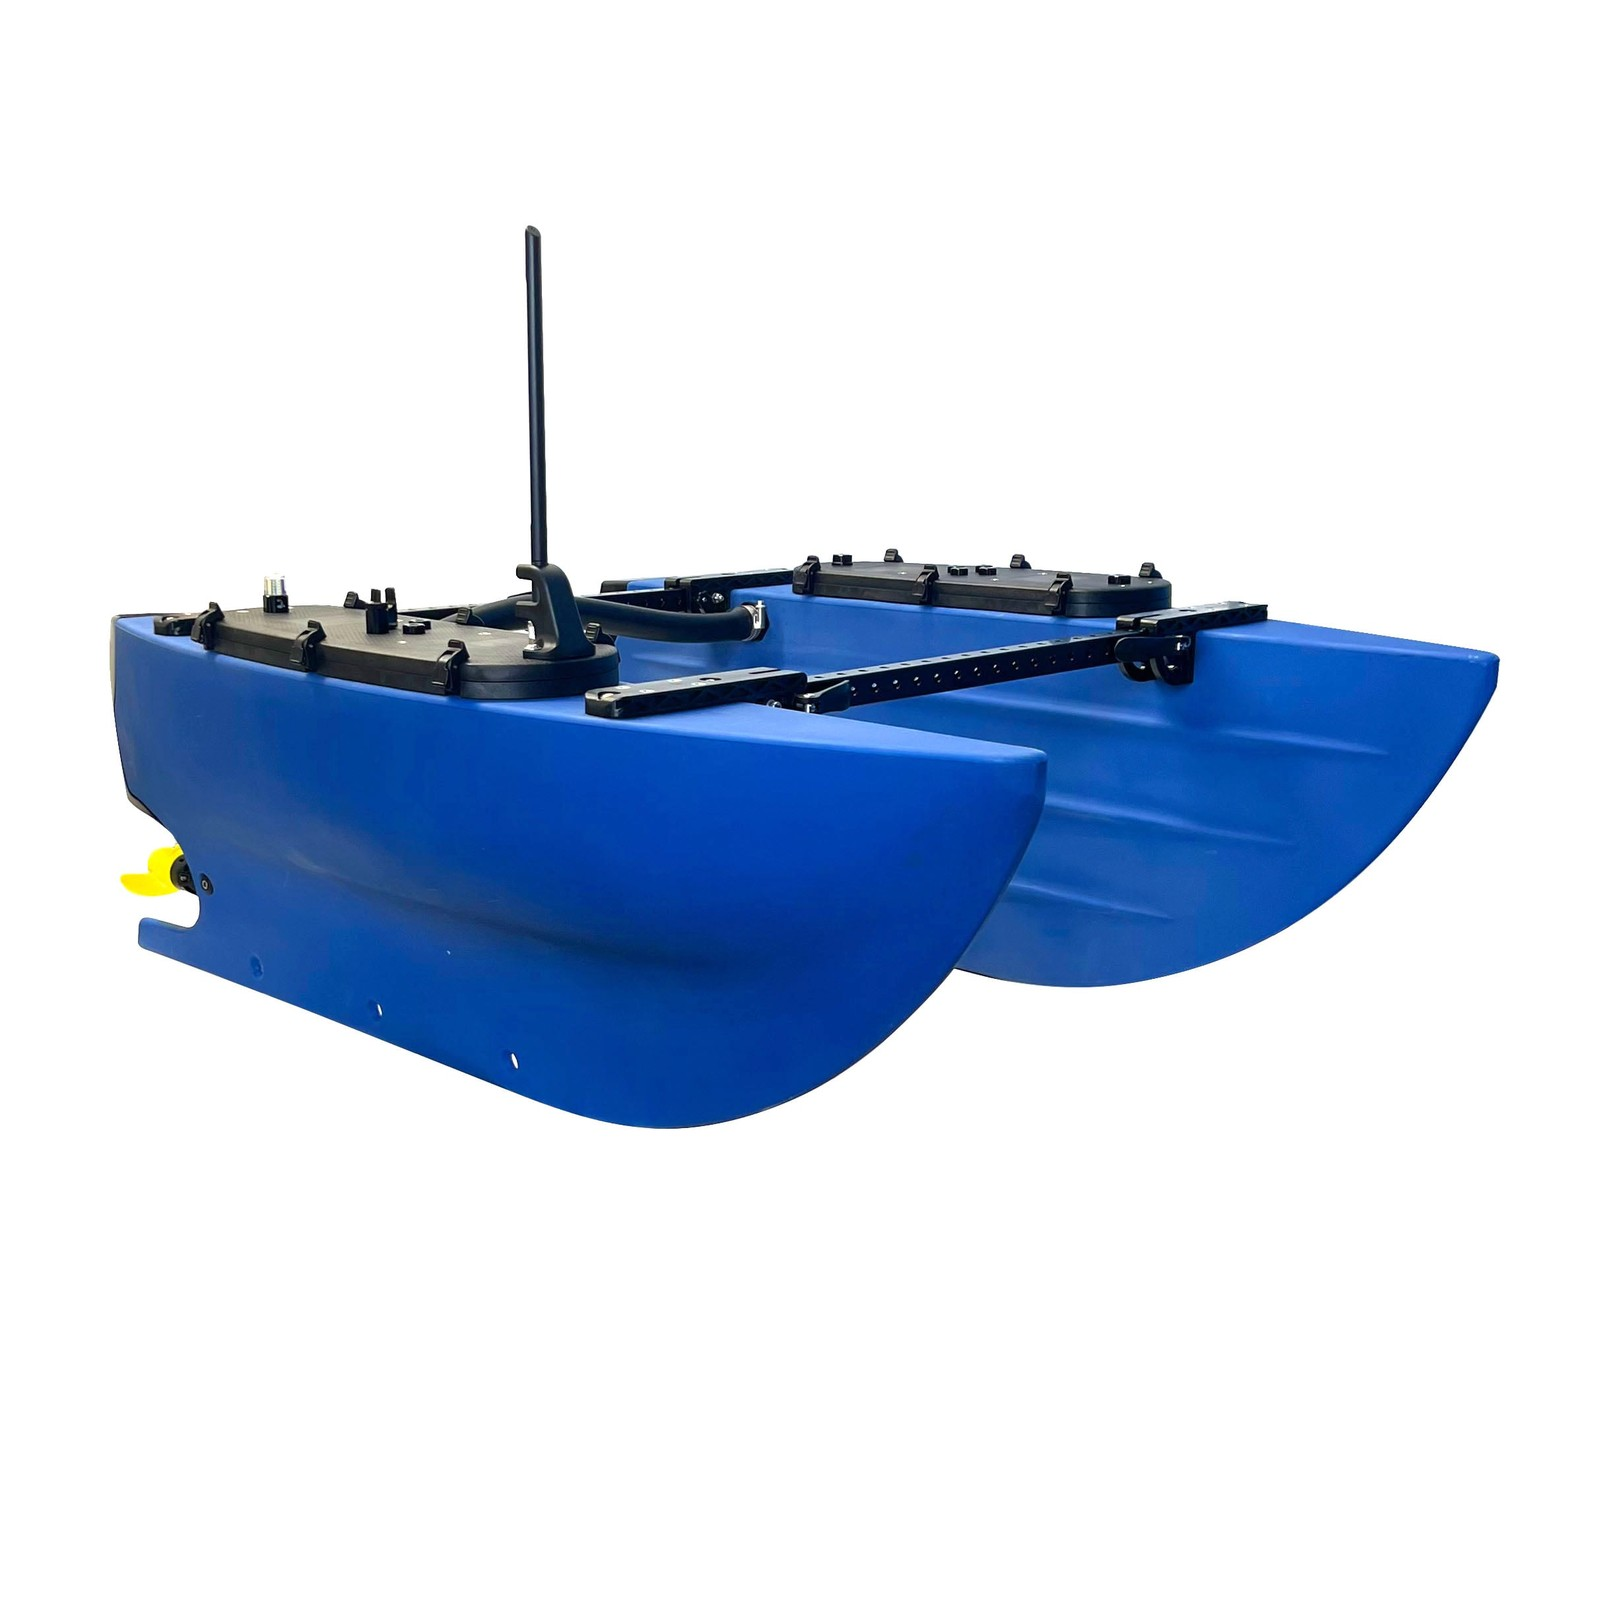
\includegraphics[height=2.0cm, keepaspectratio]{blueboat.jpg}\\
        \vspace{0.15em}
        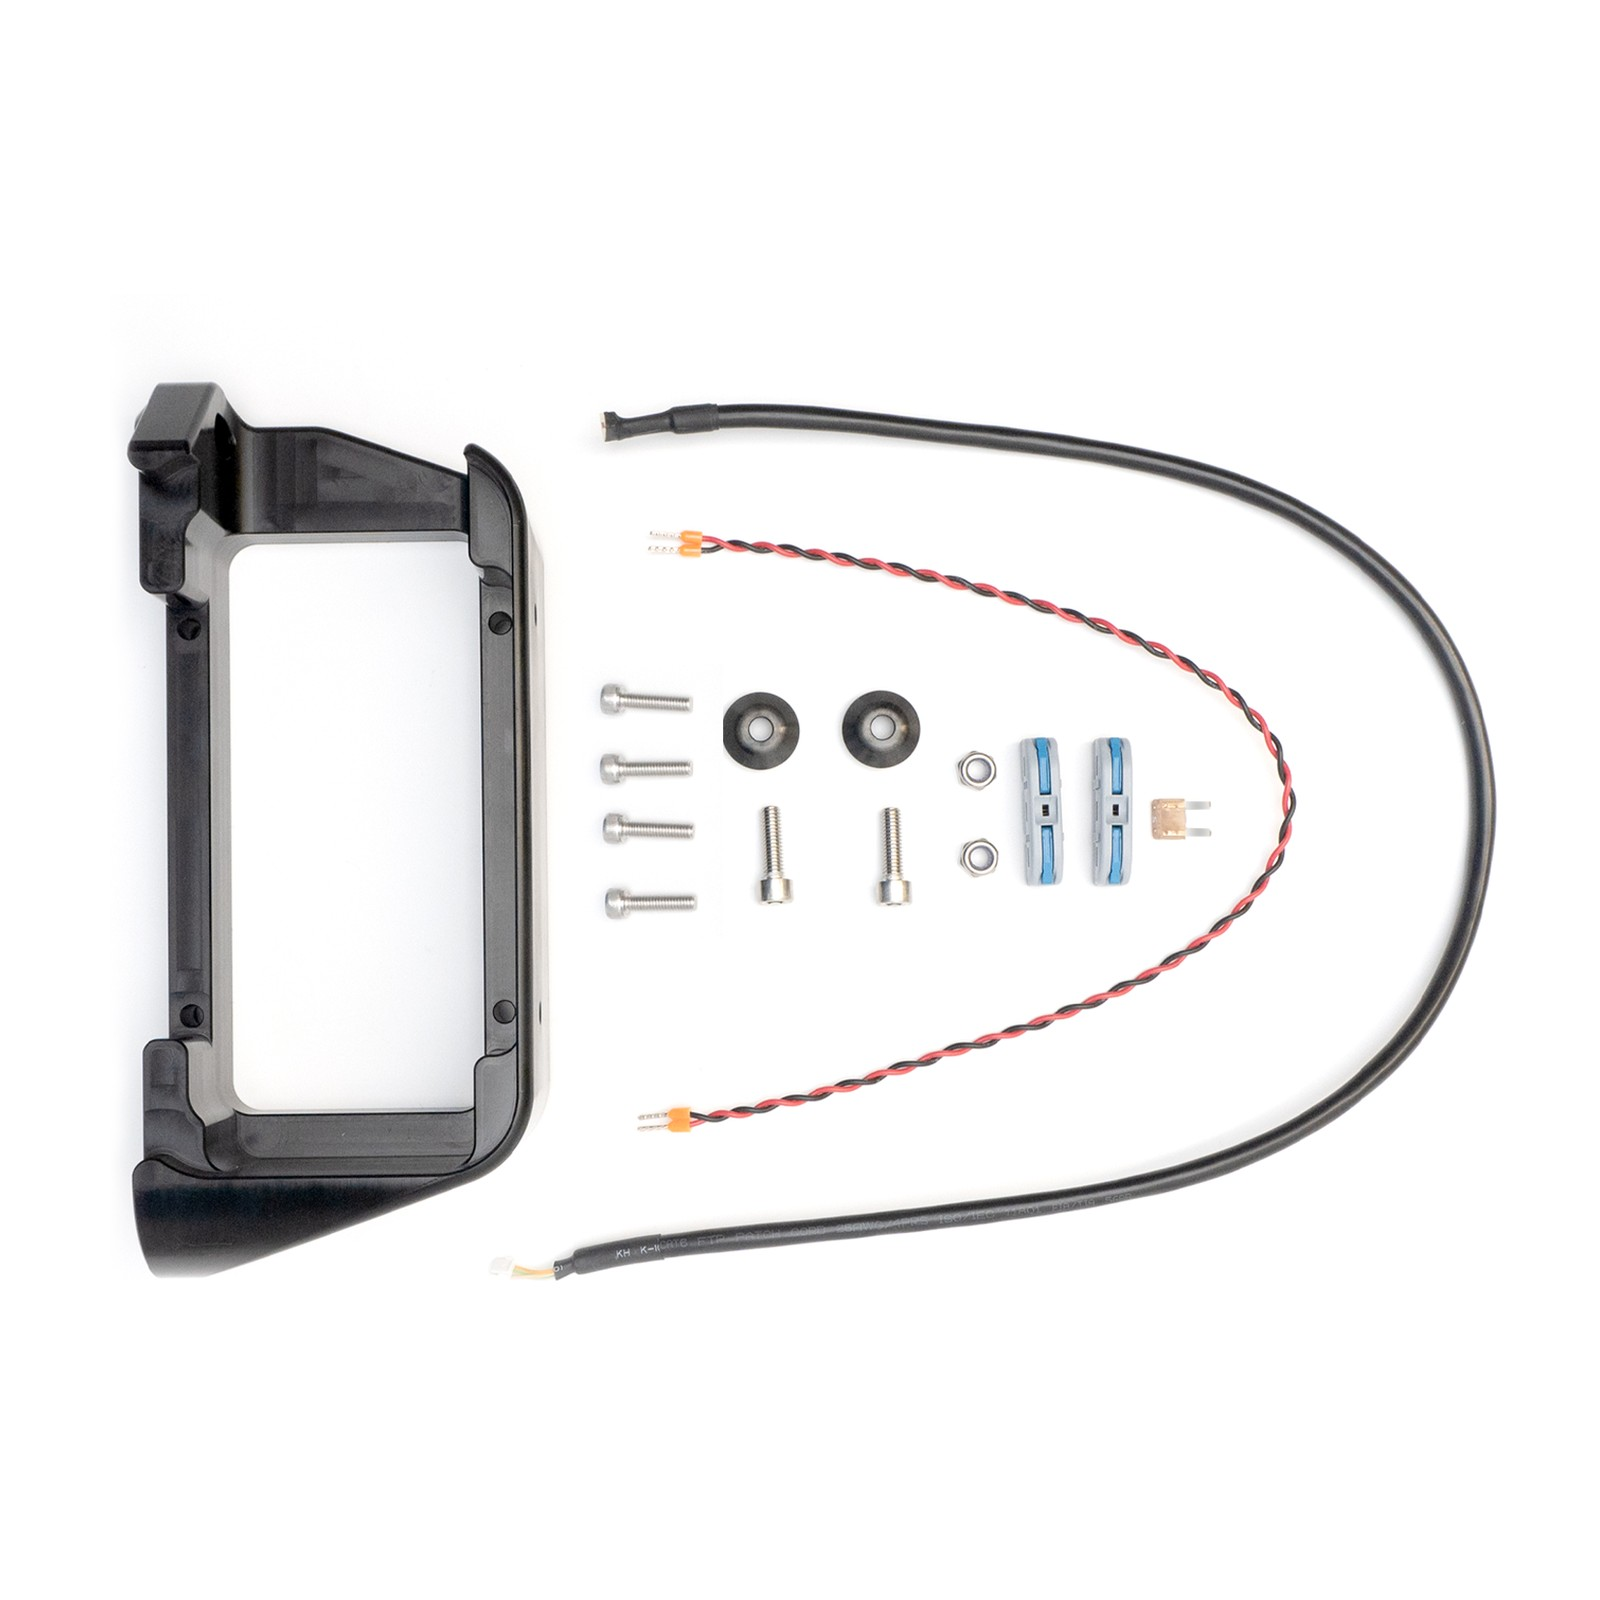
\includegraphics[height=1.7cm, keepaspectratio]{cerulean_surveyor_mbes.jpg}\\
        \vspace{0.1em}
        \scriptsize\textbf{BlueBoat} + \textbf{MBES Surveyor 240-16}
      \end{center}
    \end{column}

    \begin{column}{0.62\textwidth}
      \textbf{Cartographie bathymétrique \& physico-chimique} :
      \scriptsize
      \begin{itemize}
        \item Coque catamaran BlueBoat pilotée par \tech{ArduRover}.
        \item \textbf{Positionnement centimétrique} : GNSS RTK connecté au réseau public \succw{Centipede RTK}.
        \item \textbf{Sondeur sous coque} : Ping Sonar ou Cerulean Surveyor (MBES multifaisceaux) pour MNT 3D haute résolution.
        \item \textbf{Mission type} : tracé de transects parallèles espacés de $5\,\text{m}$, quadrillage automatique à $1.5\,\text{m/s}$ pendant 6 heures.
      \end{itemize}

      \vspace{0.3em}
      \begin{block}{Atouts Opérationnels}
        \scriptsize
        Déploiement par 1 seule personne sans grue, zéro risque d'immersion caisson, rapatriement WiFi/4G en direct au labo.
      \end{block}
    \end{column}
  \end{columns}
\end{frame}

\begin{frame}{5.3 Cas Pratique 3 : Équipe Mixte ASV-ROV (BlueBoat + BlueROV2)}
  \begin{columns}[T]
    \begin{column}{0.48\textwidth}
      \begin{center}
        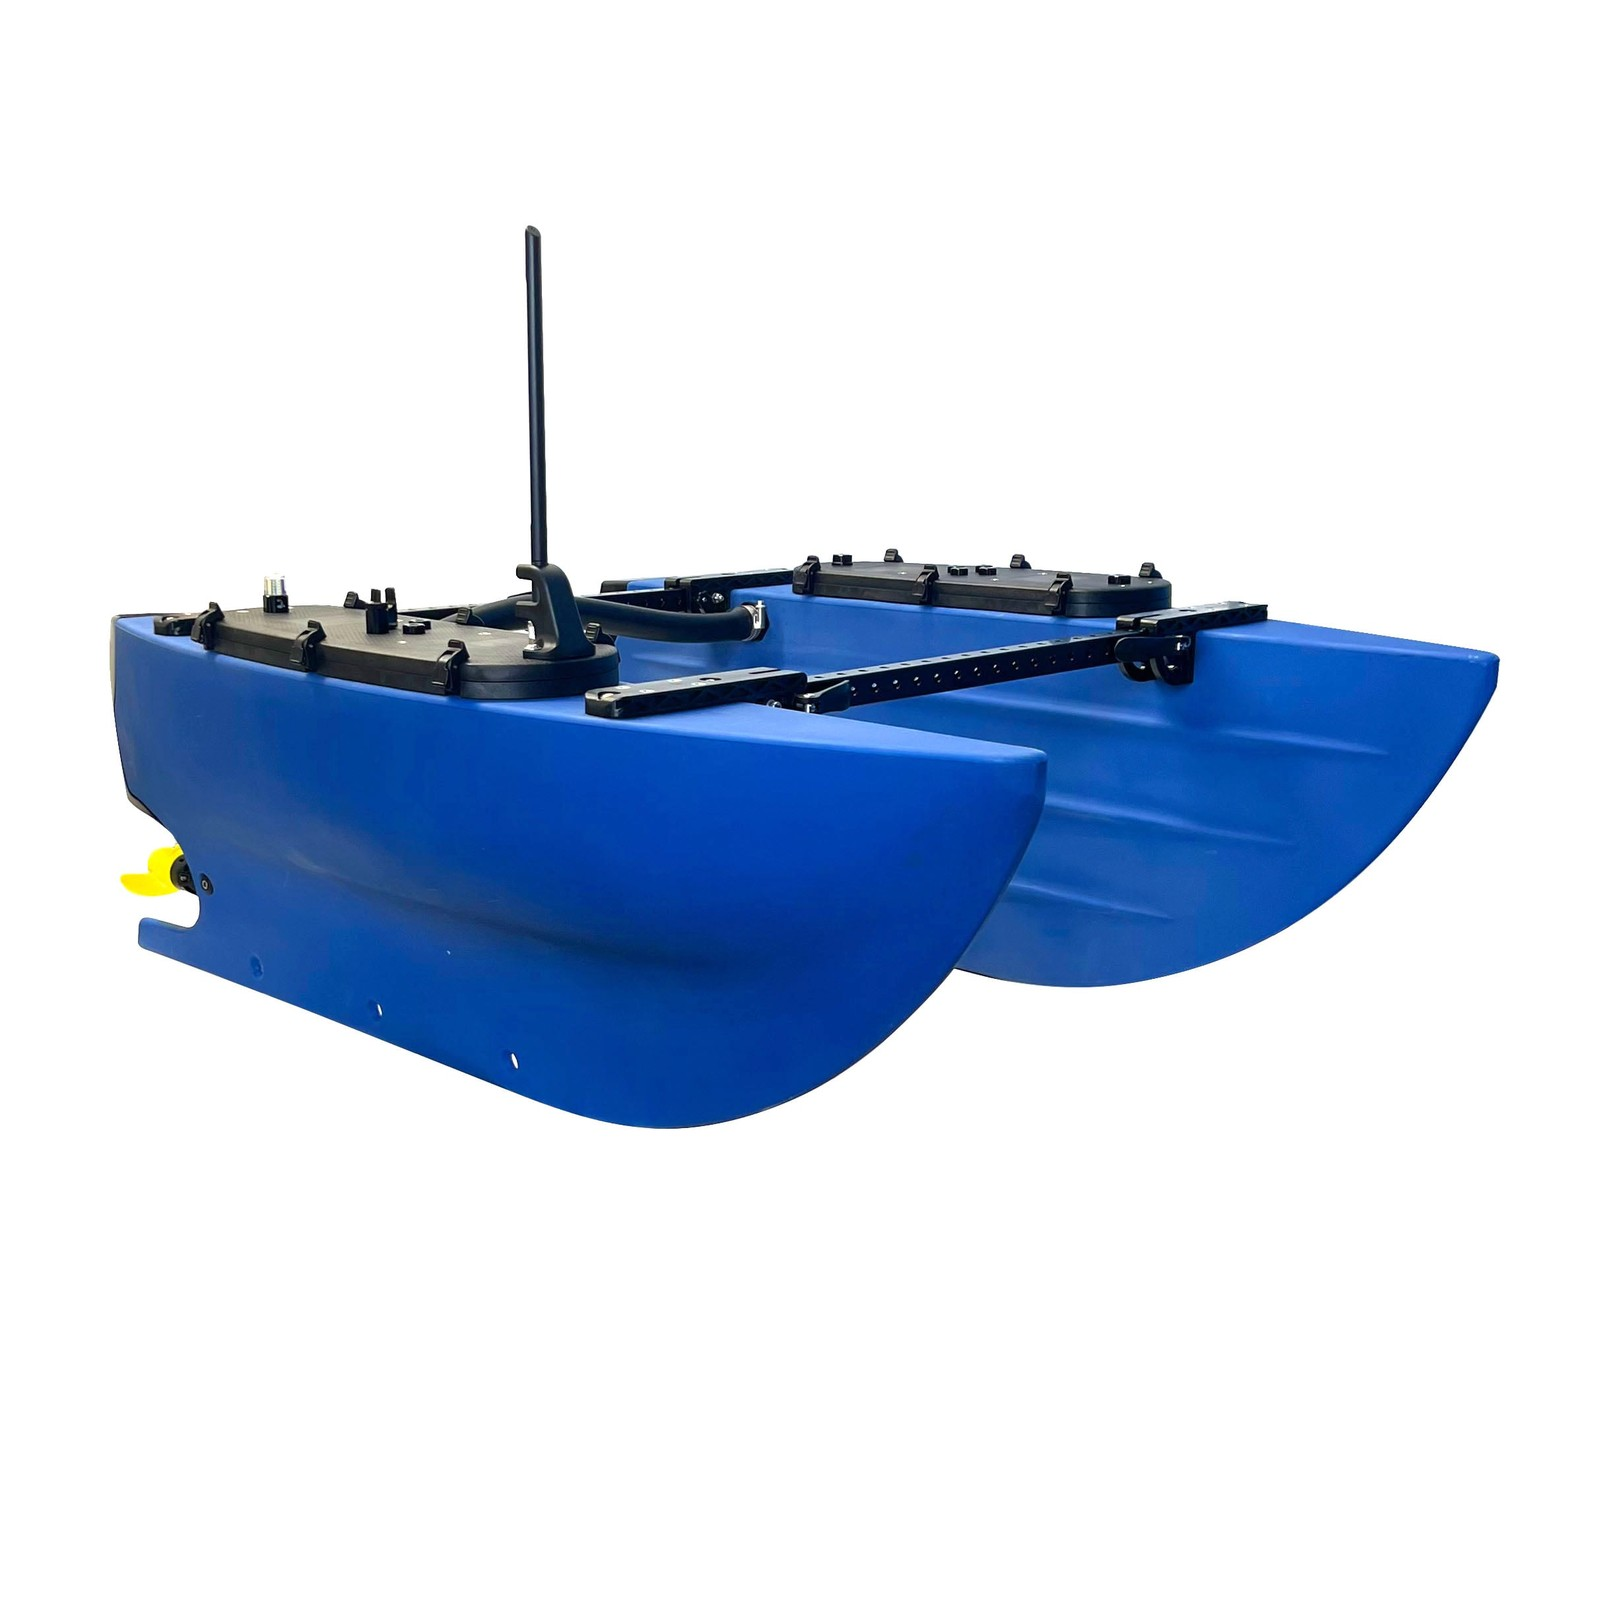
\includegraphics[height=1.5cm, keepaspectratio]{blueboat.jpg}
        \hspace{0.2cm}
        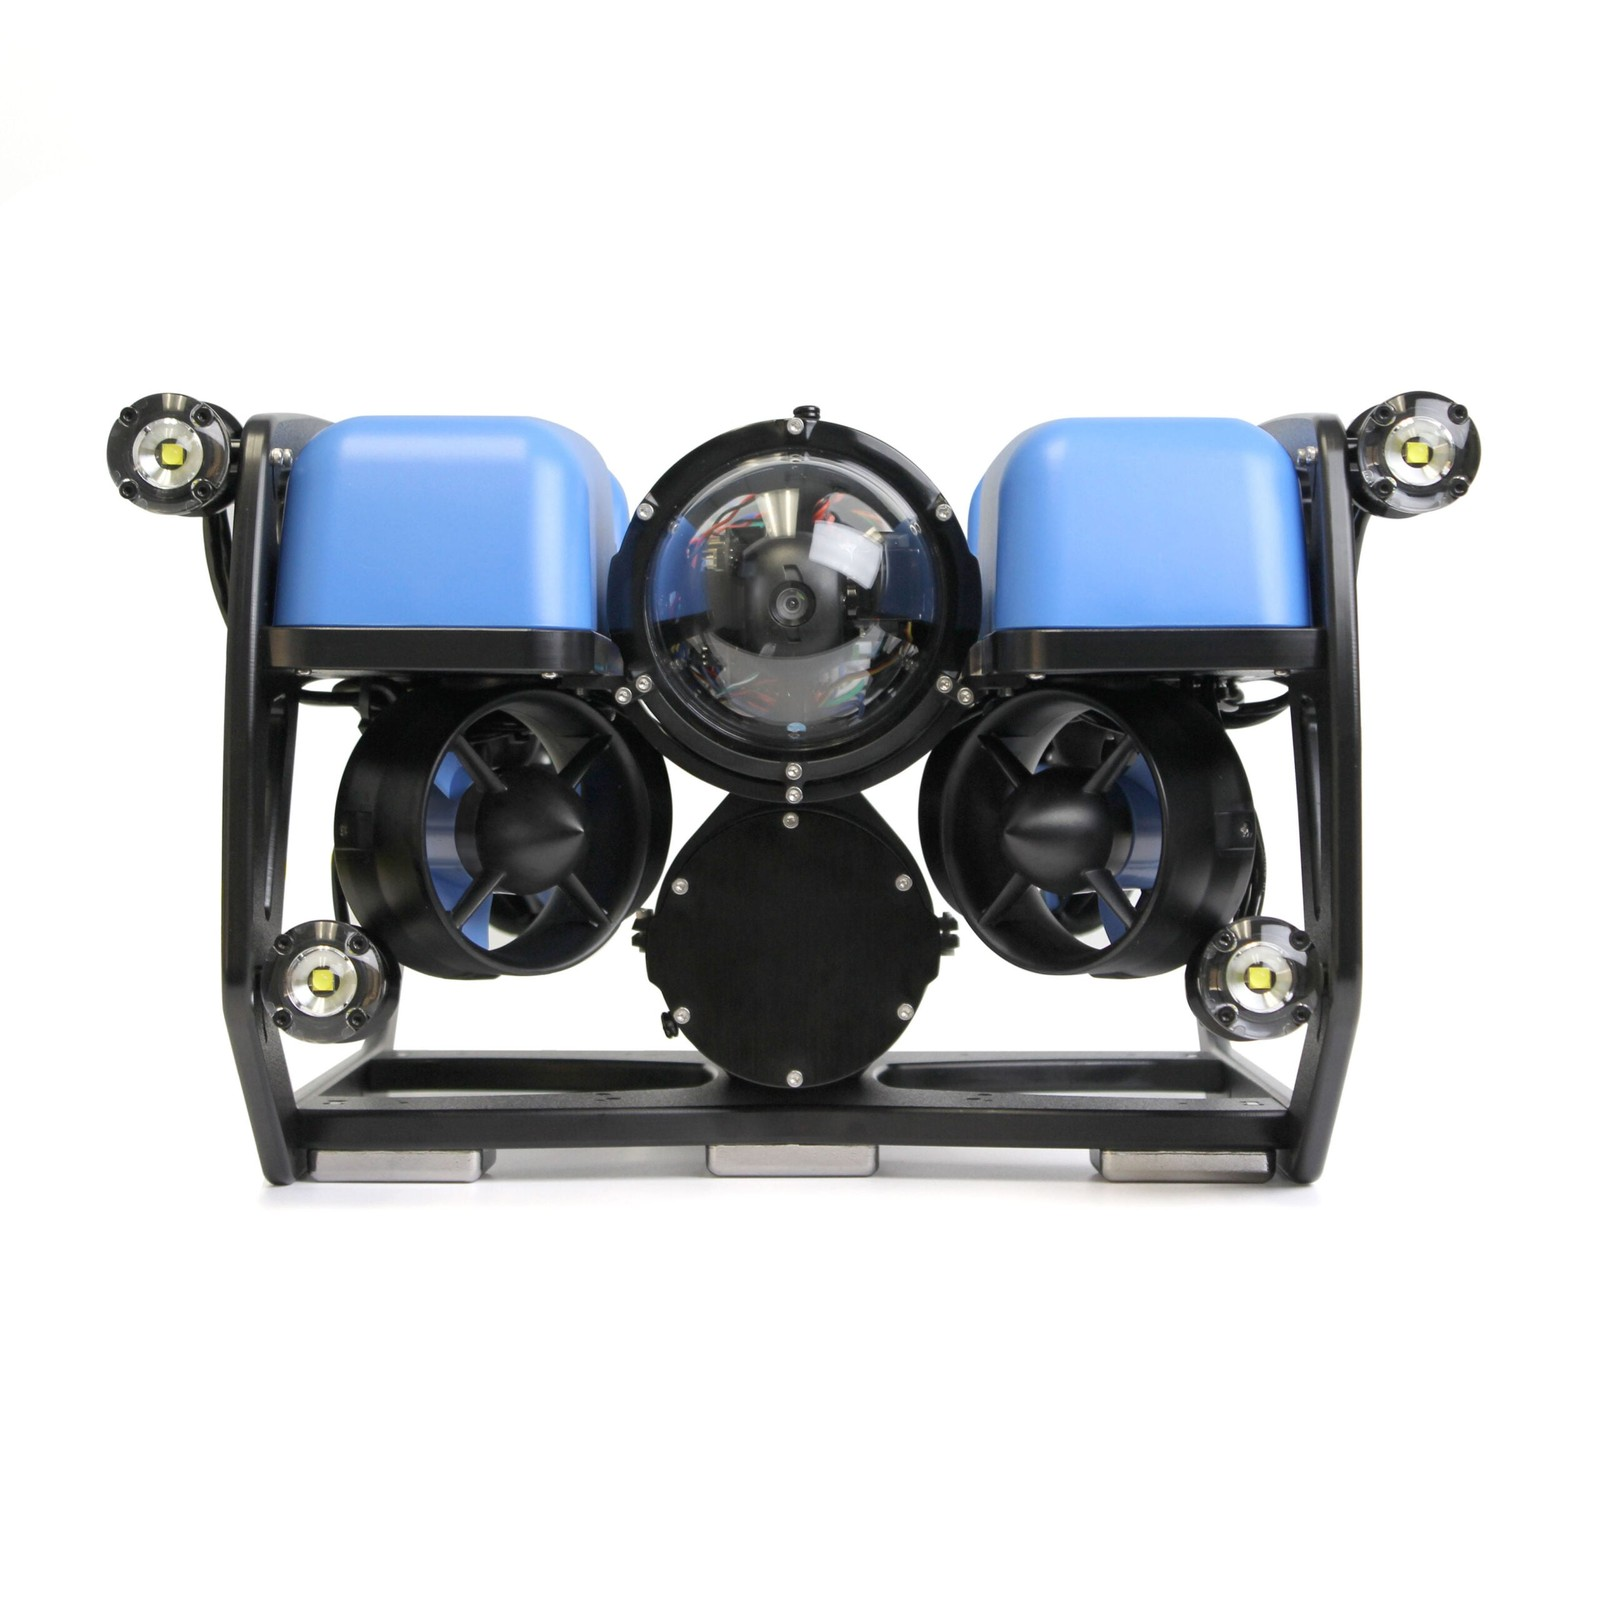
\includegraphics[height=1.5cm, keepaspectratio]{bluerov2.jpg}\\
        \vspace{0.1em}
        \tech{Drone de Surface ASV (BlueBoat)} + \succw{ROV Subaquatique (BlueROV2)}
      \end{center}
      \scriptsize
      \begin{block}{Le Cœur du Concept : La Passerelle de Surface}
        \begin{itemize}
          \item Le \textbf{BlueBoat} (ASV) navigue de façon autonome sur la zone d'étude grâce au positionnement \textbf{GNSS}.
          \item Il transporte éventuellement un enrouleur d'ombilical, l'antenne Wi-Fi/4G et un modem acoustique USBL.
        \end{itemize}
      \end{block}
    \end{column}

    \begin{column}{0.50\textwidth}
      \begin{exampleblock}{Avantages de l'Équipe Mixte Air-Surface-Fond}
        \scriptsize
        \begin{itemize}
          \item \textbf{Déploiement à grande élongation} : l'ASV amène le ROV sur site sans mobiliser de navire de recherche lourd avec équipage.
          \item \textbf{Relais de données haut débit} : le BlueBoat sert de répéteur radio/4G vers le laboratoire à terre.
          \item \textbf{Recalage absolu} : l'ASV injecte sa position GNSS RTK par USBL dans l'estime du BlueROV2.
        \end{itemize}
      \end{exampleblock}
    \end{column}
  \end{columns}
\end{frame}

\begin{frame}{5.4 Cas Pratiques Innovants : MAUV \& Flagellator}
  \begin{columns}[T]
    \begin{column}{0.47\textwidth}
      \begin{center}
        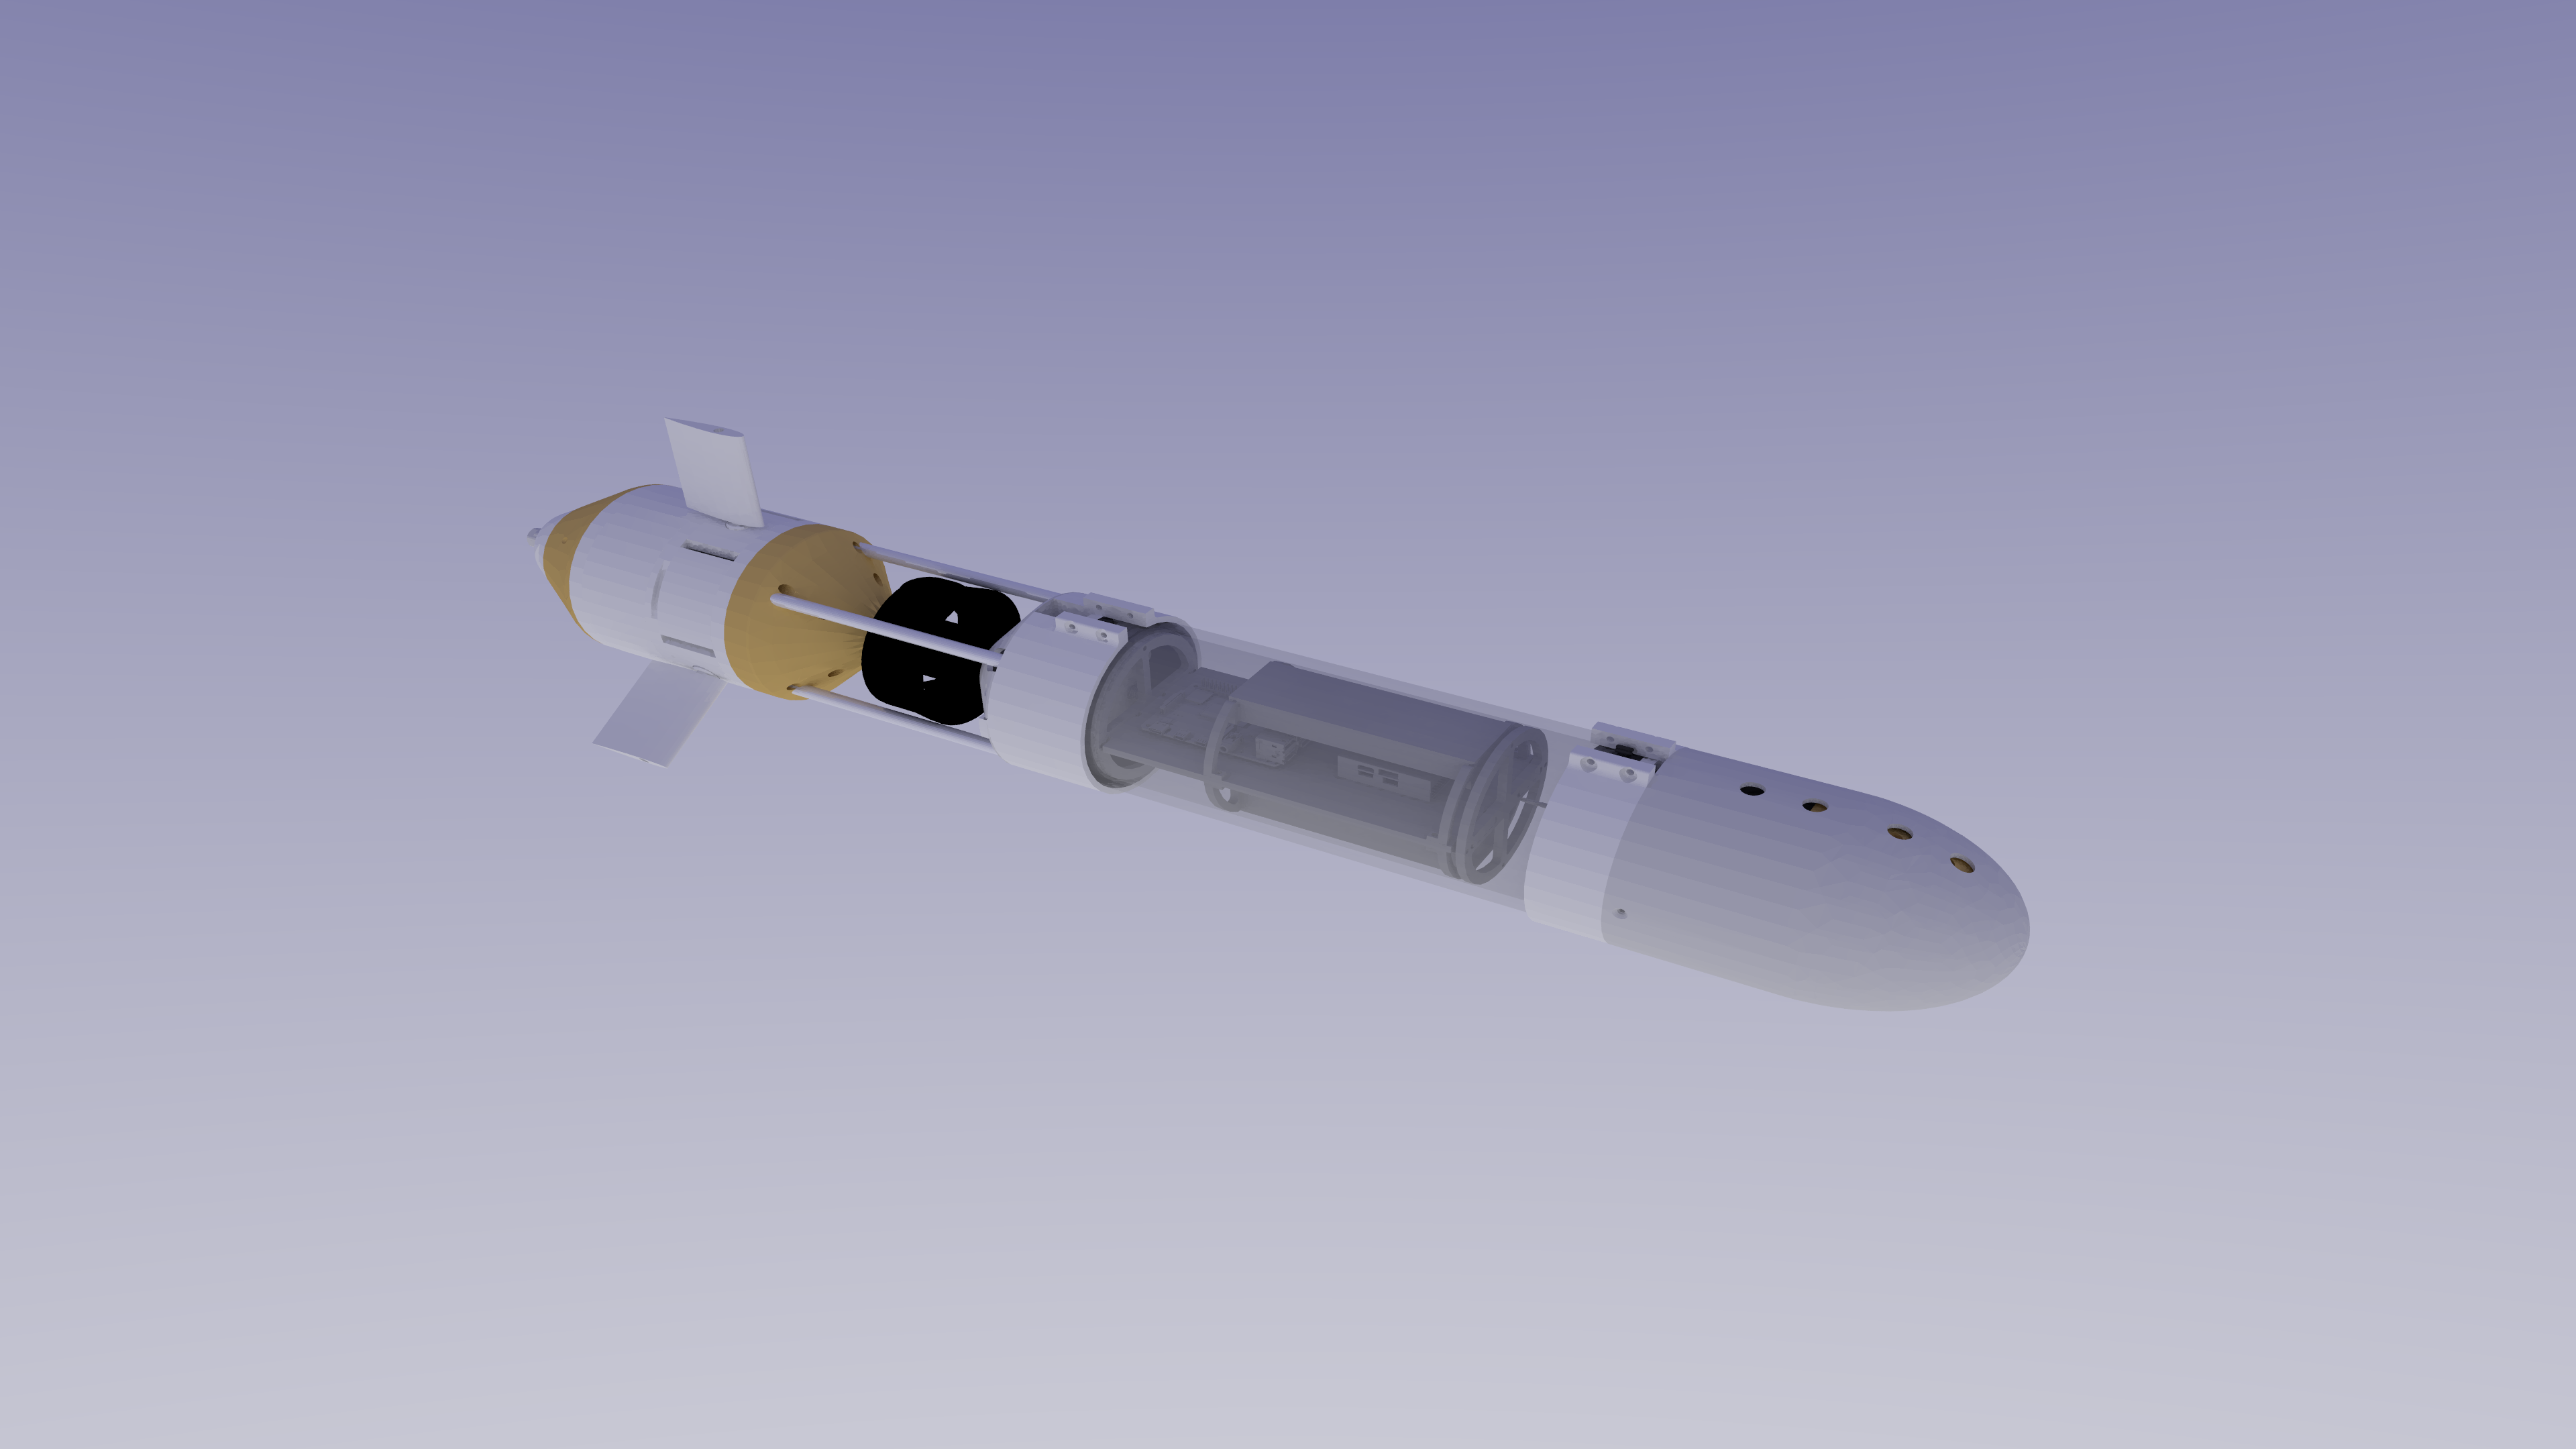
\includegraphics[height=2.1cm, keepaspectratio]{mauv.png}\\
        \vspace{0.1em}
        \tech{Modular-AUV (MAUV)}\\
        \tiny\textit{Vecteur sous-marin modulaire ultra-léger}
      \end{center}
      \scriptsize
      \begin{itemize}
        \item \textbf{Concept MAUV} : sous-marins ultra-léger ($<15\,\text{kg}$).
        \item \textbf{Man\oe uvrant} : propulseur placé devant les ailerons pour générer un flux d'eau permettant de tourner à vitesse très faible.
      \end{itemize}
    \end{column}

    \begin{column}{0.47\textwidth}
      \begin{center}
        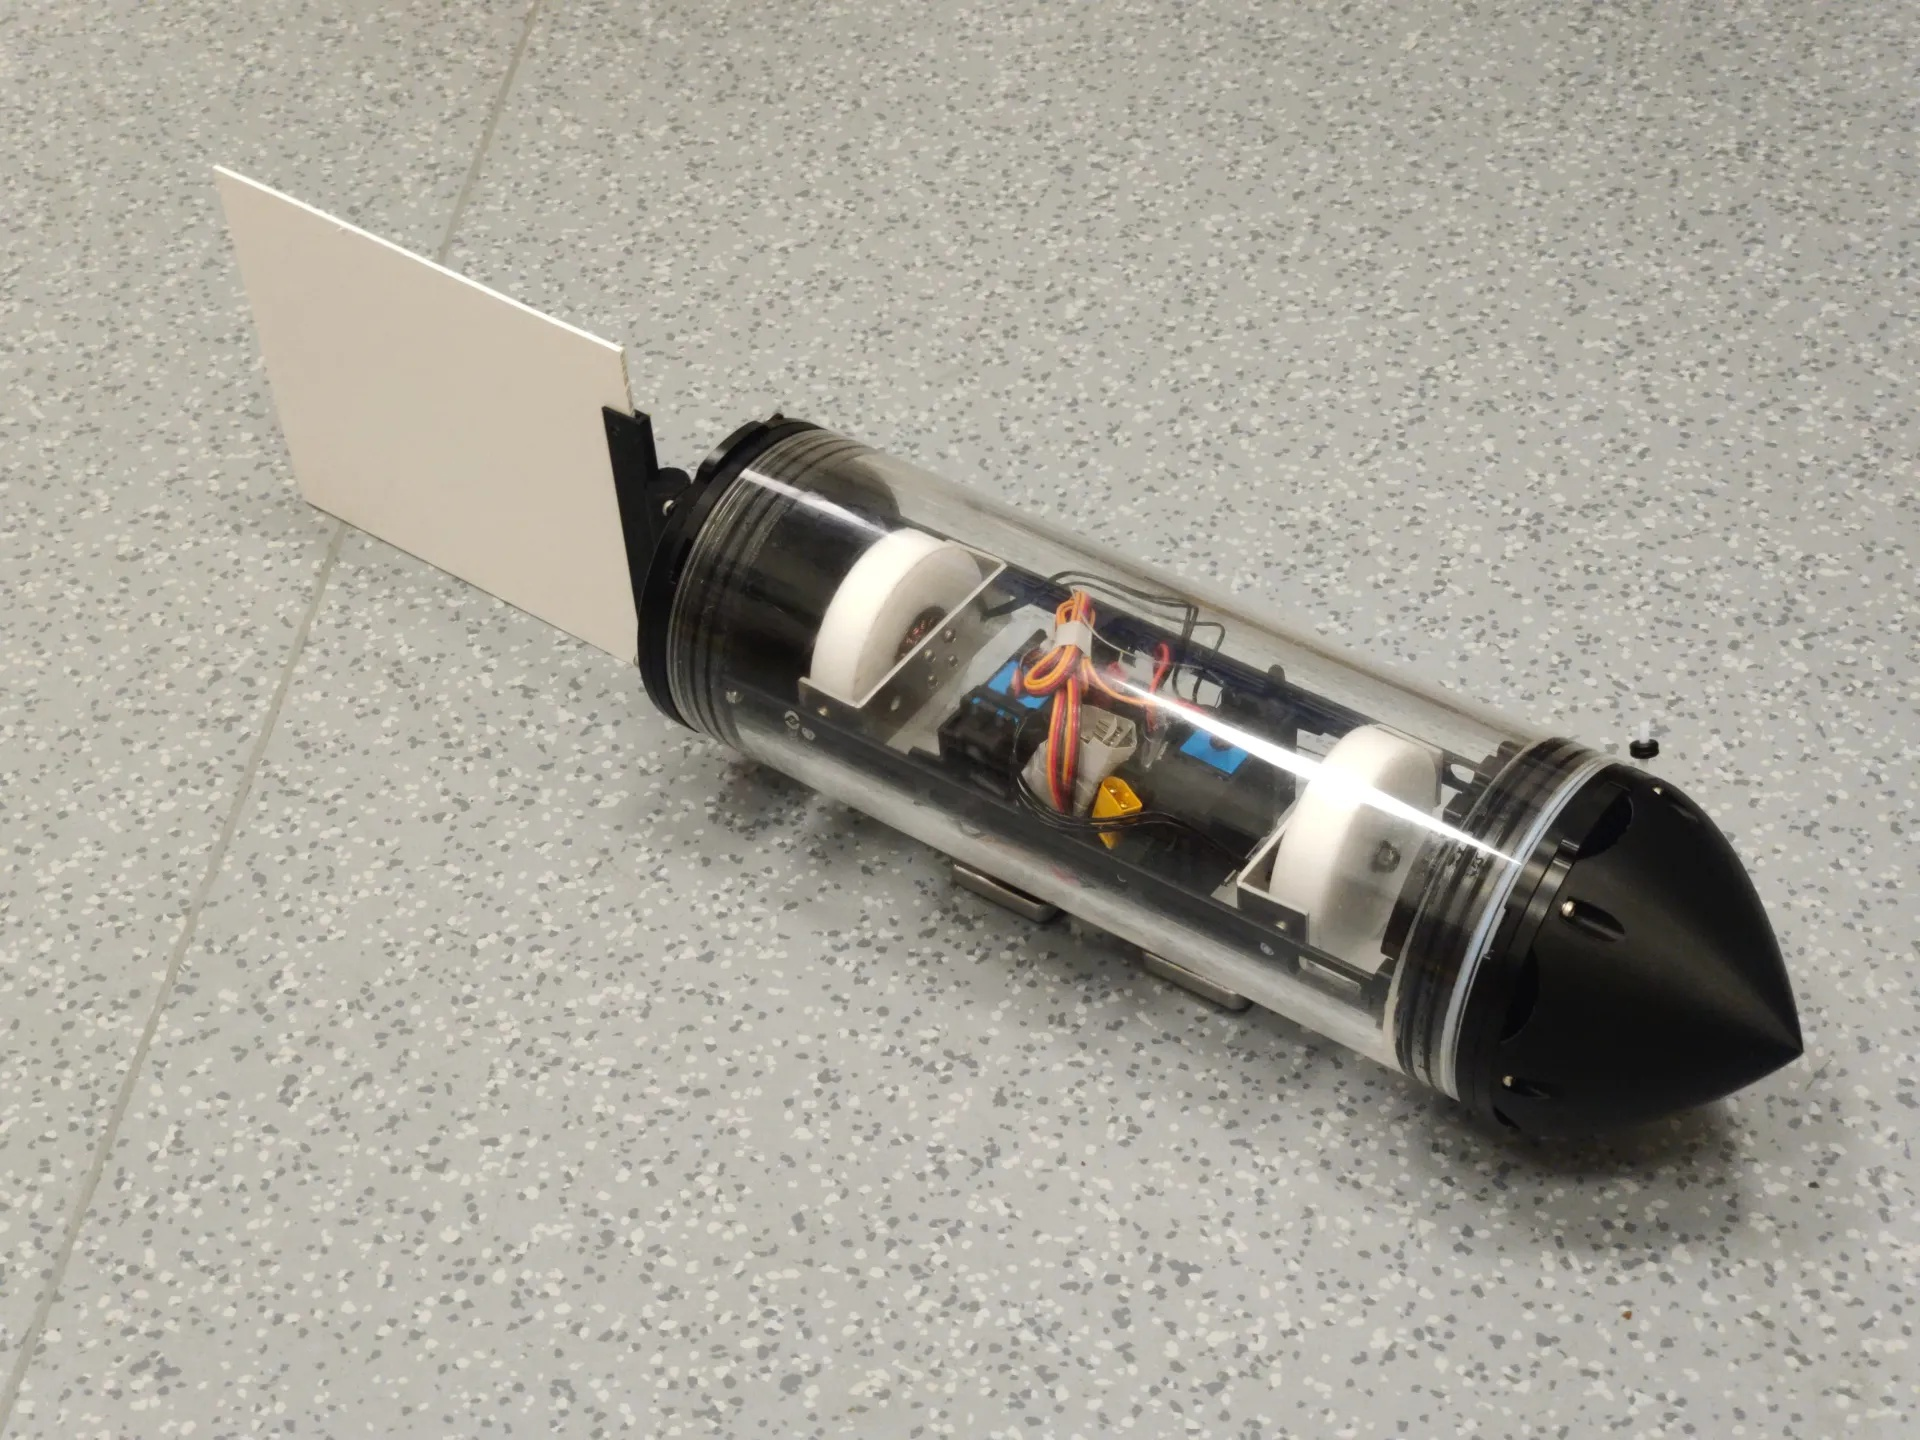
\includegraphics[height=2.1cm, keepaspectratio]{flagellator.jpg}\\
        \vspace{0.1em}
        \alertw{Le Robot Bio-inspiré Flagellator}\\
        \tiny\textit{Propulsion ondulatoire flagellaire}
      \end{center}
      \scriptsize
      \begin{itemize}
        \item \textbf{Nage biomimétique} : propulsion par ondulation continue d'une membrane/flagelle déformable.
        \item \textbf{Zéro hélice contondante} : intégrité et sécurité absolue lors des interventions près de la faune ou des récifs fragiles.
        \item \textbf{Pas d'étanchéité} : absence de passage de cable pour les actionneurs.
      \end{itemize}
    \end{column}
  \end{columns}
\end{frame}

\begin{frame}{5.4 Atelier Collaboratif : À Vous la Parole !}
  \begin{block}{Tour de table des projets scientifiques Drone\&Cap' \& 2RM}
    Présentez en 2 minutes votre problématique d'instrumentation :
    \begin{itemize}
      \item Quel est votre \textbf{milieu d'étude} ? (lagune côtière, récif corallien, fleuve turbide, lac de haute montagne).
      \item Quelles sont les \textbf{grandeurs physiques} à mesurer ? (bathymétrie, herbiers, turbidité, traceurs chimiques, profils CTD).
      \item Quel est le compromis optimal : \textbf{ROV filaire}, \textbf{AUV autonome} ou \textbf{ASV de surface} ?
    \end{itemize}
  \end{block}

  \vspace{0.6em}
  \begin{exampleblock}{Questions \& Réponses Ouvertes}
    \begin{itemize}
      \item Conseils sur l'approvisionnement et l'intégration mécanique/logicielle.
      \item Retours d'expérience sur les pièges à éviter lors des premières campagnes en mer.
      \item Partage de briques logicielles au sein des réseaux Drone\&Cap' et 2RM.
    \end{itemize}
  \end{exampleblock}

\end{frame}


% Slide de fin / remerciements (Standout Metropolis)
\begin{frame}[standout]
  \textbf{\Large Merci pour votre attention !}\\[1.2em]
  {\normalsize Place aux échanges et discussions pour vos projets.}\\[2em]
  {\scriptsize
  \textbf{Quentin Brateau} --- ANF ArchiDrone 2026\\
  \textit{Réseaux Drone\&Cap' \& 2RM (Réseau Métier des Roboticiens et Mécatroniciens)}}
\end{frame}

\end{document}

